\begin{refsection}
\chapter{Testing of Laser Written Emitters and Simulations} % better naming required since this is the second experimental chapter now
\begin{comment}\section{Introduction}
\subsection{Summary of Previous Experimental Work}
Chapter \ref{ch:electrical_experiments} examines the formation of conventional metal contacts to heavily phosphorous doped diamond, via annealed titanium-based contacts. The literature best-case value for the specific contact resistivity with titanium contacts is $10^{-3}$~\si{\ohm\centi\metre\squared} \cite{matsumoto2013}, as previously described in (reference to comparison of metal contacts on phosphorous doped diamond). The contacts formed in this work, both in the CTLM and LTLM experiments and under different annealing conditions, differ markedly from these examples. (final numbers for measured contact resistance here). Following these observations, it was clear that an alternative approach must be taken to form superior ohmic contacts on these samples which are sufficient to allow for competitiveness between diamond based power devices and current best case values on standard materials. For example, SiC is able to achive extremely low resistance ohmic contacts below $1\times10^{-7}$~\si{\ohm\centi\metre\squared} \cite{pan2013}.

\subsection{Improved Contacts to Diamond Devices}
Novel approaches to the formation of ohmic contacts with n-type diamond are an ongoing area of research, with unique orientation and substrate dependent methodologies being developed. For instance, \cite{temahuki2017} demonstrated the ability of Ni-catalysed etching to provide pyramidal \hkl(111) oriented pits for a heavily phosphorous doped overgrowth layer. This method provides both geometrically enhanced emitter-type structures, as well as a greater phosphorous concentration than what is otherwise obtainable on a \hkl(100) oriented substrate, hence producing significantly improved contacts than other contacts to n-type \hkl(100) substrates without micro-structures. For \hkl(111) oriented substrates, the results of various metal contact formations are summarised in (reference to comparison of metal contacts on phosphorous doped diamond). While much work in this area treats these metal contacts as ohmic in nature due solely to the nature of the heavy n-type doping and subsequent formation of titanium carbide contacts, unique approaches to further reducing this specific contact resistivity can be seen in \cite{matsumoto2013} and \cite{valappil2022}, \cite{valappil2023}. In the first such case, thermal graphitisation of the diamond surface is used to provide an additional intermediate layer for the formation of ohmic contacts, achieving an order of magnitude reduction in the specific contact resistivity when compared to the titanium carbide contacts \cite{matsumoto2013}. In the more recent work by Valappil et al, coaxial arc plasma deposition (CAPD) is used to form nanocarbon electrodes which show a similar order of magnitude improvement over the conventional titanium contacts.

One technique that has not yet been utilised for the reduction in specific contact resistivity on heavily phosphorous doped diamond is that of laser graphitisation. The utilisation of laser processing offers numerous advantages over the procedures of nanocarbon CAPD, or thermal graphitisation, such as the ability to directly pattern working contacts without standard photolithography steps, the ability to write 3D structures such as wires passing through the diamond substrate for diamond detectors \cite{bloomer2020}, and the ability to also create waveguides within the diamond substrates through modification of the local refractive index \cite{courvoisier2016}. While unrelated to power electronic applications, it is also worth noting that this process can also be used to generate point defects within diamond substrates, which can be used to generate single negatively charged nitrogen-vacancy (NV$^{-}$) centres, and have a wide array of potential applications in magnetometry, single photon sources, quantum centres, etc. \cite{chen2016}. The combination, or specific usage of any of these key features allows for a large range of device structures to be fabricated by laser graphitisation processes. For a complete review of laser graphitisation, please see chapter \ref{ch:laser}.

\subsection{Field Effect Emission}
\label{subsec:field_effect_emission}
A device structure that may particularly benefit from 3D laser graphitisation is that of the cold-cathode type structure. As described in the seminal work \cite{spindt1976}, it is possible to induce cold-field effect emission with sufficiently sharp (geometrically enhanced) structures. This structure was then proposed to be used in conjunction with the negative electron affinity of hydrogen-terminated diamond \cite{geis1996}, allowing for lower applied voltages to generate practical electron sources that could compete with thermionic emitters. Significant issues with this design structure arise during the fabrication of such structures, due in large part to the etching process and overgrowth of heavily n-type diamond. Parallels could be drawn between the fabrication of these structures and the work of \cite{temahuki2017}, where a random distribution of Ni-etched pits are overgrown with heavily phosphorous doped diamond, and finally contacted with standard Ti/Au contacts. However the fabrication of emitters as in Geis et al. requires the emitters to be fabricated such that the tips are perpendicular and very close to the surface of the diamond emitters. Any spacing between the tip of the cathode-emitter and the hydrogen terminated diamond surface will result in a large potential difference drop between the cathode and the anode, reducing the effective field strength at the tip and hence significantly affecting the field effect emission of such a device. In practice, this narrow spacing is extremely difficult to achieve via etching, as dislocations or other defects in the diamond substrate will generate fault lines for the etching process, drastically altering the etching rate. Several alternative approaches have been attempted in recent history, with a full summary provided in chapter \ref{ch:diamond}. Significantly, several devices have been suggested which attempt to either create sharp diamond cathodes, etching back substrates, or utilising designs that allow for carbon nanotubes to be employed. There is a notable overlap in device designs that attempt to fabricate emitters based on diamond and graphite, carbon nanotubes, diamond-like carbon layers, or diamondoid monolayers, all of which were designed prior to the development of 3D laser graphitisation processes. Ultimately, all such devices present insufficient properties or flaws, and this area of research is ongoing.

\subsection{Laser Written Geometrically Enhanced Emitters}
A natural proposition for 3D micron scaled laser graphitised wires within diamond such as that demonstrated within \cite{sun2014} is that of cold-cathode type devices. While a practical device that can compete with either one of the aforementioned designs or silicon-based devices is ambitious, as the phosphorous doped CVD growth of diamond and the laser graphitisation processes continue to mature, future devices which make use of these capabilities to generate cold-cathode structures with only one laser processing step may start to appear achievable. This would eliminate the need for many of the processing steps such as the deposition of Ti-C based ohmic contacts, or the need for various etching steps and differing metal depositions to produce sufficient gate electrodes in the triode structure. It also addresses the issue of thin electronic grade diamond samples being required for a suitably narrow region between the emitters and the hydrogen terminated diamond surface, which brings about a host of practical processing concerns. Also note that the requirement of electronic grade diamond for carefully controlled, reliable etching procedures is also tentatively eliminated, as the priority can instead be given to high quality phosphorous doped diamond substrates, benefiting the reduction of Schottky barrier height at the graphite/diamond interface.

Hence, experimental work was planned to examine both the effect of laser processing for the purpose of reduced specific contact resistivity ohmic contacts, and to also explore the possibility of laser written structures utilising an emitter type design.

\subsection{Graphitised Device Design}

\begin{figure}[H]
    \centering
    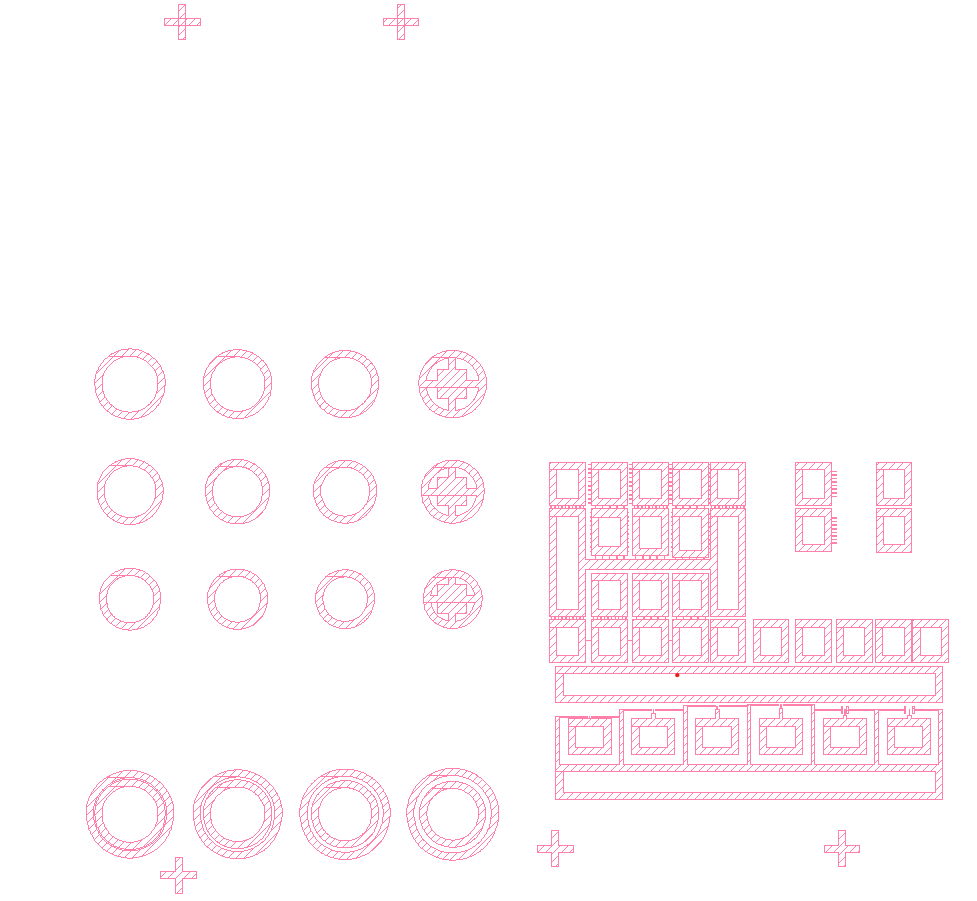
\includegraphics[width=\textwidth]{Chapter7/Figs/Raster/overview of design.png}
    \caption{An overview of the laser graphitisation design, including alignment markers for potential photolithography steps and various device structures as described in this section.}
    \label{fig:design_overview}
\end{figure}

To test the reduction of specific contact resistivity via laser graphitisation and the preliminary concept of laser graphitised emitters, the laser graphitisation layout as shown in figure \ref{fig:design_overview} was designed. Various strategies were employed to allow for the testing of various specific features. Of particular note are the LTLM structures, CTLM structures and the emitter array seen as an array of rectangular contacts. This allowed for some redundancy in the devices, and the direct comparison between different devices. The best example of this is between the LTLM array, which is a simple rectangular arrangement of contacts with channel spacings between 2--9~\si{\micro\metre}, and the emitter arrays, which had similar rectangular contacts to the LTLM array, but with protruding emitters between the two contacts. The comparison between planar contacts and these geometrically enhanced contacts can then be compared to look for signs of field effect emission due to the sharp emitter features.

\begin{figure}[h]
    \centering
    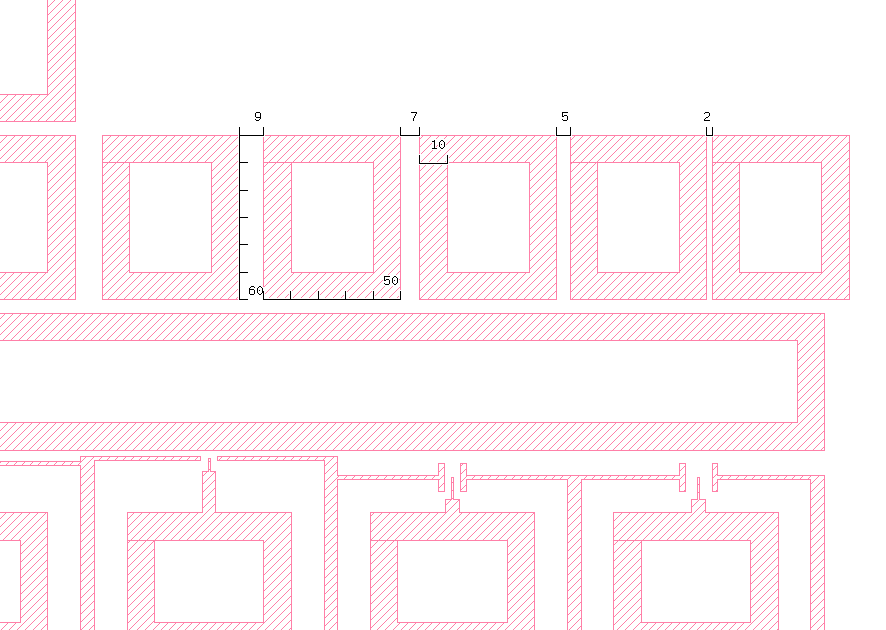
\includegraphics[width=\textwidth]{Chapter7/Figs/Raster/zoom1 LTLM area.png}
    \caption{A close up of the LTLM design, including scale measurements of relevant feature sizes for clarity.}
    \label{fig:design_ltlm }
\end{figure}\end{comment}

\subsection{Emitter Sharpness}
\label{subsec:emitter_sharpness}
In designing the emitter-type structures, the plausibility of measuring field effect emission was examined via electrostatic FEM in Comsol Multiphysics. The most critical factor to consider in these simulations was that of the effective cathode tip. Previous work in Oxford has demonstrated conductive graphite wires going down to 400~\si{\nano\metre} in diameter \cite{sun2014}, however the creation of sharp emitters depends upon the cross-sectional area presented at the very end of such a wire. Simple electrostatic simulations were created to estimate the magnitude of the normal electric field experienced by wires ranging from rectangular in appearance with very sharp corners, to wires with the corners tapered off to such a degree that the radius of curvature aligns with the wire diameter. Following these electrostatic models, implementation of Fowler-Nordheim type field-effect emission (outlined in chapter \ref{ch:semiconductors_and_diamond} was implemented to estimate the emitted current corresponding to the normal electric field on the cathodes.

\begin{figure}[H]
    \centering
    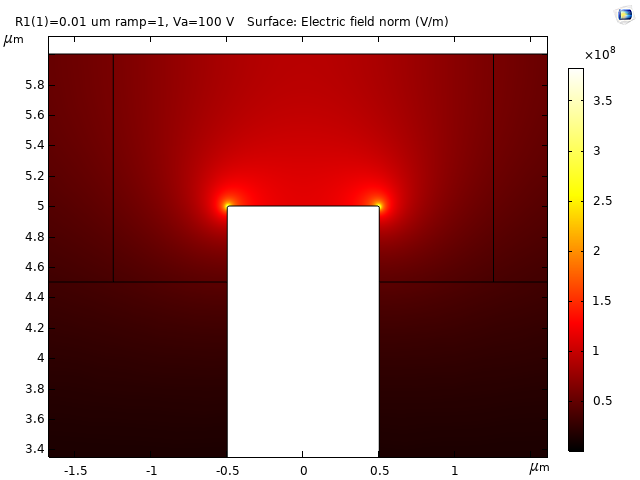
\includegraphics[width=\textwidth]{Chapter7/Figs/Raster/example structure 0.01 normE.png}
    \caption{Electrostatic modelling of a surface graphitic wire with diameter 1~\si{\micro\metre} and corner radii of 0.01~\si{\micro\metre}.}
    \label{fig:comsol_es_wire0.01}
\end{figure}

Figure \ref{fig:comsol_es_wire0.01} illustrates the electrostatic profile of a surface graphitic wire of diameter 1~\si{\micro\metre}, which has very sharp corners which have radii of curvature of 0.01~\si{\micro\metre}. The 2D model is performed with a thickness of 1~\si{\micro\metre}. Note the intensely localised electric field at the corners of the wire, reaching above $3.5\times10^{8}$~\si{\volt\per\metre}, with significantly lower normal electric fields across the rest of the wire. In this model, the cathode is held at 0~\si{\volt}, while the anode is held at 100~\si{\volt}. The cathode-anode spacing is 1~\si{\micro\metre}. The segmented sections visible (black lines) indicate different regions of meshing, with a very dense mesh used for the region immediately surrounding the tip of the emitter to better resolve the sharper features.

\begin{figure}[H]
    \centering
    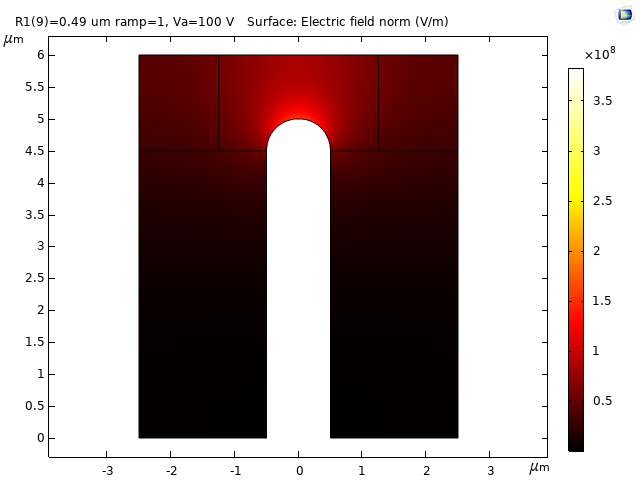
\includegraphics[width=\textwidth]{Chapter7/Figs/Raster/example structure 0.49 normE.png}
    \caption{Electrostatic modelling of a surface graphitic wire with diameter 1~\si{\micro\metre} and corner radii of 0.49~\si{\micro\metre}.}
    \label{fig:comsol_es_wire0.49}
\end{figure}

Figure \ref{fig:comsol_es_wire0.49} demonstrates the electrostatic profile of a surface graphitic wire of diameter 1~\si{\micro\metre}, which has corners of radii 0.49~\si{\micro\metre}. The 2D model is performed with a thickness of 1~\si{\micro\metre}. Note that in contrast to figure \ref{fig:comsol_es_wire0.01}, the wire in this model has corner radii which are very close to the radius of the wire, resulting in a nearly semi-circular end to the wire. The resulting normal electric field is significantly more diffuse than in the low radii example, with a peak at the very end of the wire corresponding to around $1.5\times10^{8}$~\si{\volt\per\metre}. In this model, the cathode is held at 0~\si{\volt}, while the anode is held at 100~\si{\volt}. The cathode-anode spacing is 1~\si{\micro\metre}. The segmented sections that are partially visible (black lines) indicate different regions of meshing, with a very dense mesh used for the region immediately surrounding the tip of the emitter to better resolve the sharper features.

\begin{figure}[H]
    \centering
    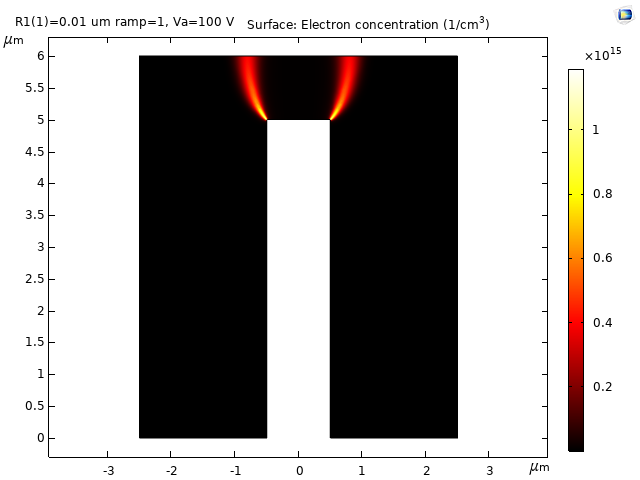
\includegraphics[width=\textwidth]{Chapter7/Figs/Raster/FN radius 0.01 width 1um 100V 0V.png}
    \caption{Fowler-Nordheim modelling of a surface graphitic wire with diameter 1~\si{\micro\metre} and corner radii of 0.01~\si{\micro\metre}.}
    \label{fig:comsol_fn_wire0.01}
\end{figure}

In figure \ref{fig:comsol_fn_wire0.01}, a 2D simulation of a surface graphitic emitter-type structure is shown. Following a Fowler-Nordheim type field-effect emission, the resulting electron concentration can be seen to be heavily emitted from the corners, which have radii of 0.01~\si{\micro\metre}. Notable differences from the previous electrostatic modelling include the implementation of n-type doping corresponding to TLM measurements (exact concentration was what again? maybe refer to section in which I establish modelling and include the TLM models there) and a standard thermionic Schottky barrier at the cathode-diamond interface with the addition of Fowler-Nordheim tunnelling. For more details regarding the computational implementation of Fowler-Nordheim barriers, please see section (bit on meshing, Schottky barriers, some more plots of simple devices, etc. also maybe get better plots of these models, all files still saved no reason why not. normalised colour scale?). The peak electron concentration for this model was just over $1\times10^{15}$~\si{\per\centi\metre\cubed}, which is present at the corners, dropping off rapidly as the peak electric field drops following the electrostatic model of figure \ref{fig:comsol_es_wire0.01}.

\begin{figure}[H]
    \centering
    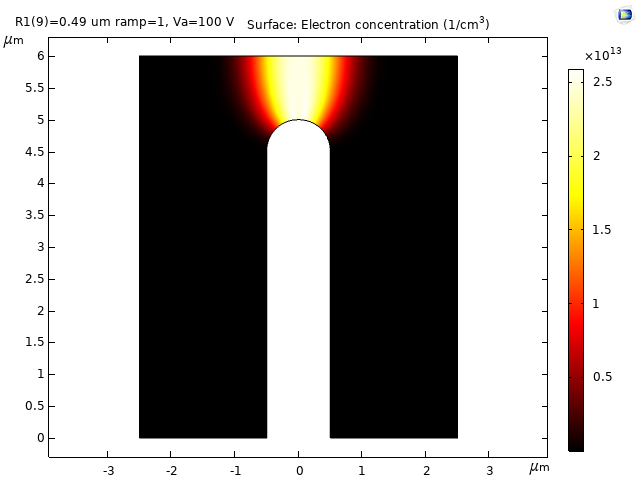
\includegraphics[width=\textwidth]{Chapter7/Figs/Raster/FN radius 0.49 width 1um 100V 0V.png}
    \caption{Fowler-Nordheim modelling of a surface graphitic wire with diameter 1~\si{\micro\metre} and corner radii of 0.49~\si{\micro\metre}.}
    \label{fig:comsol_fn_wire0.49}
\end{figure}

In figure \ref{fig:comsol_fn_wire0.49}, a 2D simulation of a surface graphitic emitter-type structure is shown. Contrasting with figure \ref{fig:comsol_fn_wire0.01}, this model has corners of radii 0.49~\si{\micro\metre}, which are very close to the radius of the wire and hence produce a semi-circular tip. (Again refer to previous section for further information of TLM determined effective concentration etc etc). As the Fowler-Norheim emission is highly sensitive to the normal electric field, the peak electron concentration is distributed across the peak of the spherical emitter tip, where a significantly wider region is actively emitting electrons at peak concentration relative to the 0.01~\si{\micro\metre} radii. The peak concentration of electrons in this larger radii case is just over $2.5\times10^{13}$~\si{\per\centi\metre\cubed}, contrasting with the $1\times10^{15}$~\si{\per\centi\metre\cubed} of the sharper case. The order of magnitude difference of 100 with only a scale difference in the peak normal electric field of around 2 demonstrates the drastic geometric enhancement that is possible for field-effect emission.
\begin{comment}
\section{Laser Graphitisation Fabrication}
Laser graphitisation of diamond surfaces allows for significant advancement in the fabrication of diamond-based electronic devices. This technique leverages focused laser beams to convert specific regions of the diamond substrate into graphitic material, facilitating the creation of conductive pathways and contacts essential for device functionality. Precise control over the graphitisation process enables the fabrication of complex structures, such as wires and contact pads, with tailored electrical properties. For a full review of this technique, see chapter \ref{ch:laser}. The laser fabrication of the following sample as tested in this chapter was performed at Oxford University in collaboration with Patrick Salter and Ravi Shivaraman, using the mask designed by the candidate.

\subsection{Laser Fabrication Processing}
The laser graphitisation process employs a state-of-the-art Pharos laser system, operating at a wavelength of 515~\si{\nano\metre}. This system is characterised by its high repetition rate of 10~\si{\kilo\hertz}, which is crucial for achieving consistent graphitisation across the targeted areas. The choice of objective lens and the adjustment of laser pulse energy play significant roles in defining the morphology and conductivity of the graphitised structures.

\subsubsection{Laser Parameters and Setup} 
The fabrication of graphitic wires and contact pads utilised objective lenses with numerical apertures (NA) of 0.75 and 0.5, respectively. The higher pulse energy facilitated by the 0.75 NA objective lens is preferred for creating wider wires, while the 0.5 NA lens is suited for processing the contact pads. Notably, the sequence in which these components are fabricated; starting with the contact pads before the wires, was observed during initial processing to influence the wire morphology, particularly near the pads. This suggests that the local thermal and structural changes induced by the pad fabrication can affect subsequent graphitisation steps.

\subsubsection{Calibration of Pulse Energy} 
The precise calibration of pulse energy is critical for optimising the graphitisation process. Although initial settings were based on angular adjustments of the waveplate, detailed calibration is necessary to correlate these settings with specific pulse energies. This calibration ensures that the laser energy delivered to the diamond surface is precisely controlled, minimising damage to surrounding areas while maximising the quality and conductivity of the graphitic structures.

\subsubsection{Significance of Laser Processing Parameters} 
\label{subsubsec:significance_of_laser_processing_parameters}
The choice of laser parameters, including the repetition rate, pulse energy, and objective lens, directly impacts the efficiency and outcome of the graphitisation process. These parameters determine the depth, width, and electrical properties of the graphitic structures, influencing the performance of the final diamond-based devices. It is also important to note that the sample used here is different to that found in previous studies, as our sample was that of a \hkl(111) oriented HPHT substrate, with a highly phosphorous doped surface layer of $\sim1$~\si{\micro\metre} thickness, wheras previous work was performed on \hkl(100) oriented, undoped CVD substrates of impurity concentration levels.

This subsection has outlined the foundational aspects of the laser graphitisation fabrication process, highlighting the critical role of laser parameters in achieving desired structural and electrical characteristics. Further characterisation techniques, such as AFM, PL, and Raman spectroscopy, provide deeper insights into the quality and properties of the graphitised diamond, which will be discussed in the subsequent sections.

\subsection{AFM Characterisation}
\label{subsec:afm_characterisation}
To characterise the surface topology of the laser graphitised devices, AFM was used to provide broad overviews of the resulting structures following the fabrication at Oxford. 

\begin{figure}[H]
    \centering
    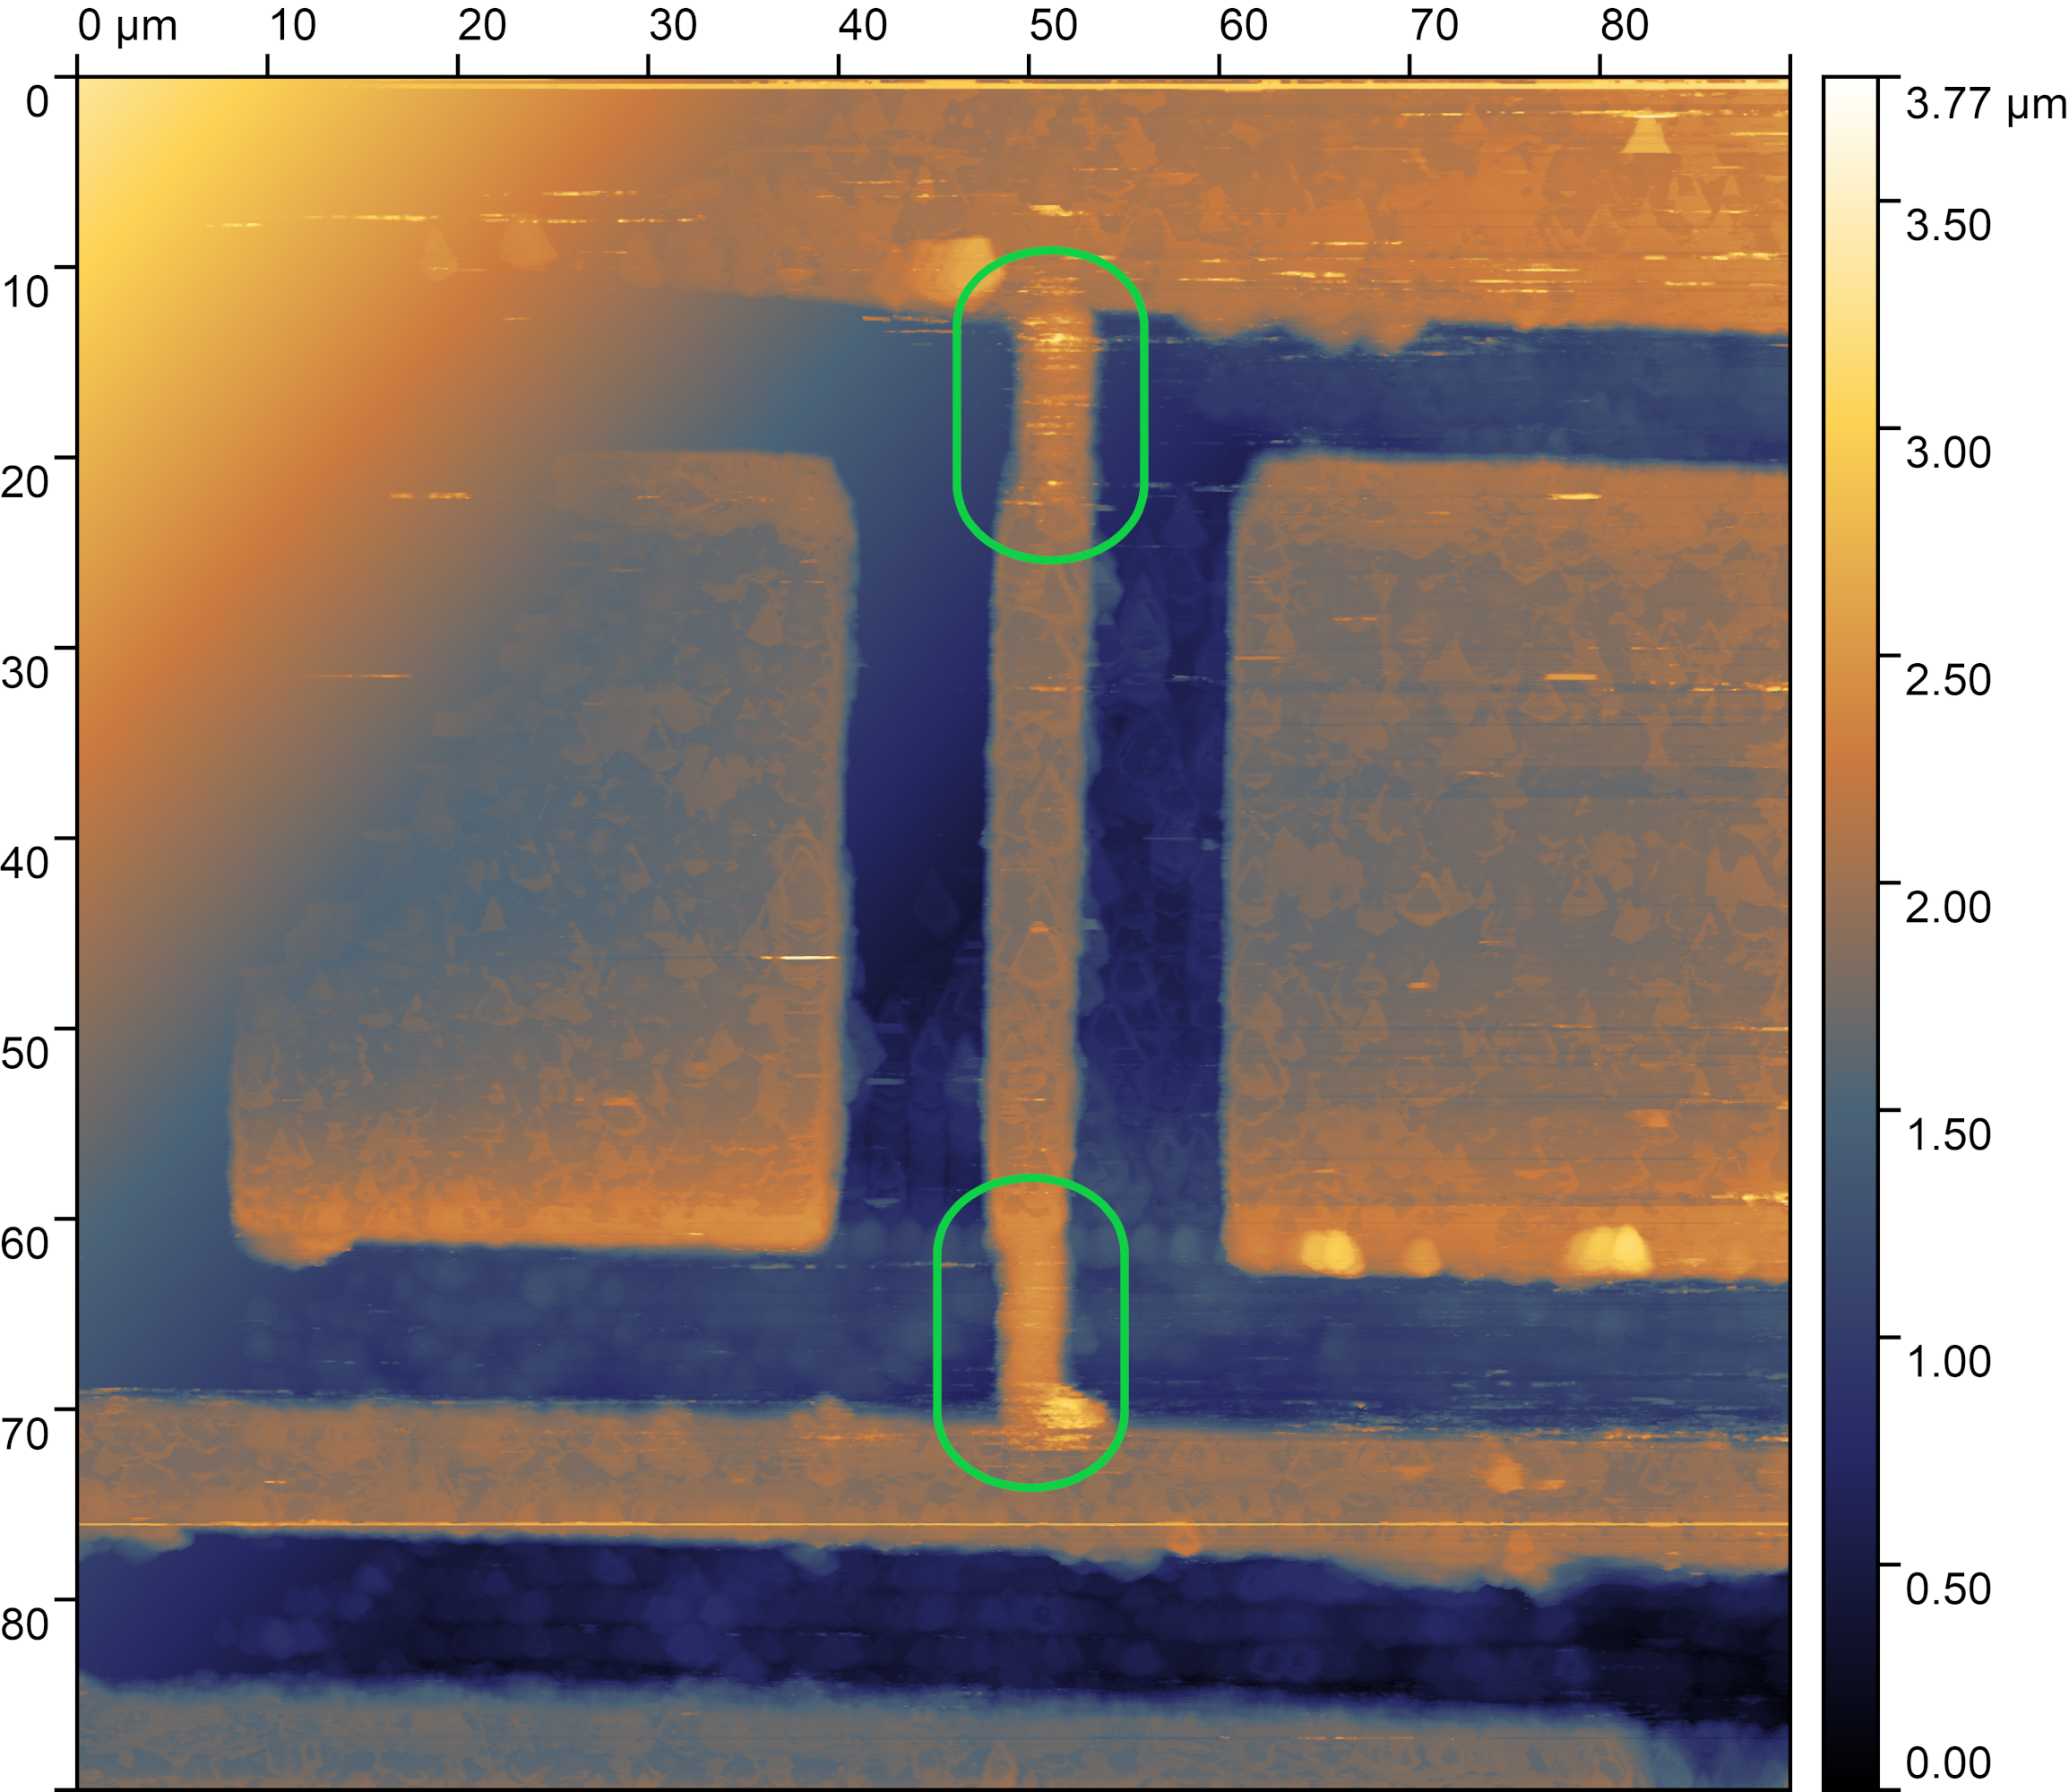
\includegraphics[width=\textwidth]{Chapter7/Figs/Raster/21 meh 4k_white_annotated_downscaled.png}
    \caption{A large area AFM scan of the LTLM channel that was designed to have a spacing of 2~\si{\micro\metre}.}
    \label{fig:afm_21_big}
\end{figure}

Figure \ref{fig:afm_21_big} shows a broad scan of the LTLM contacts that were designed to have a spacing of 2~\si{\micro\metre}. The top left corner of this scan experienced a systematic error, visible as a raised blur. Preliminary low resolution scans of this region did not contain this error, and it can hence be identified as a scanning error unrelated to the sample. Otherwise, the scan managed to achieve a generally high level of detail, despite the 90~\si{\micro\metre} square area being close to the maximum scan area for the XE-150 system. Of note is the slightly inconsistent channel length between the two rectangular contacts, presented in the exact centre of the figure. At the top and bottom of the contacts, marked by the green capsules, the channel is visibly squeezed in, with the rest of the channel presenting a thicker separation. It is also possible to see that the laser graphitisation has etched down into the diamond surface on the order of 1~\si{\micro\metre}. This presented a concern that the laser graphitisation process may have etched through the active, phosphorous doped layer of $1.2$~\si{\micro\metre}, with thin graphite walls on the edges of the ablated regions provided electrical contact, in contrast to the intended block of graphitic material in full proximity to the phosphorous doped channel.

\begin{figure}[H]
    \centering
    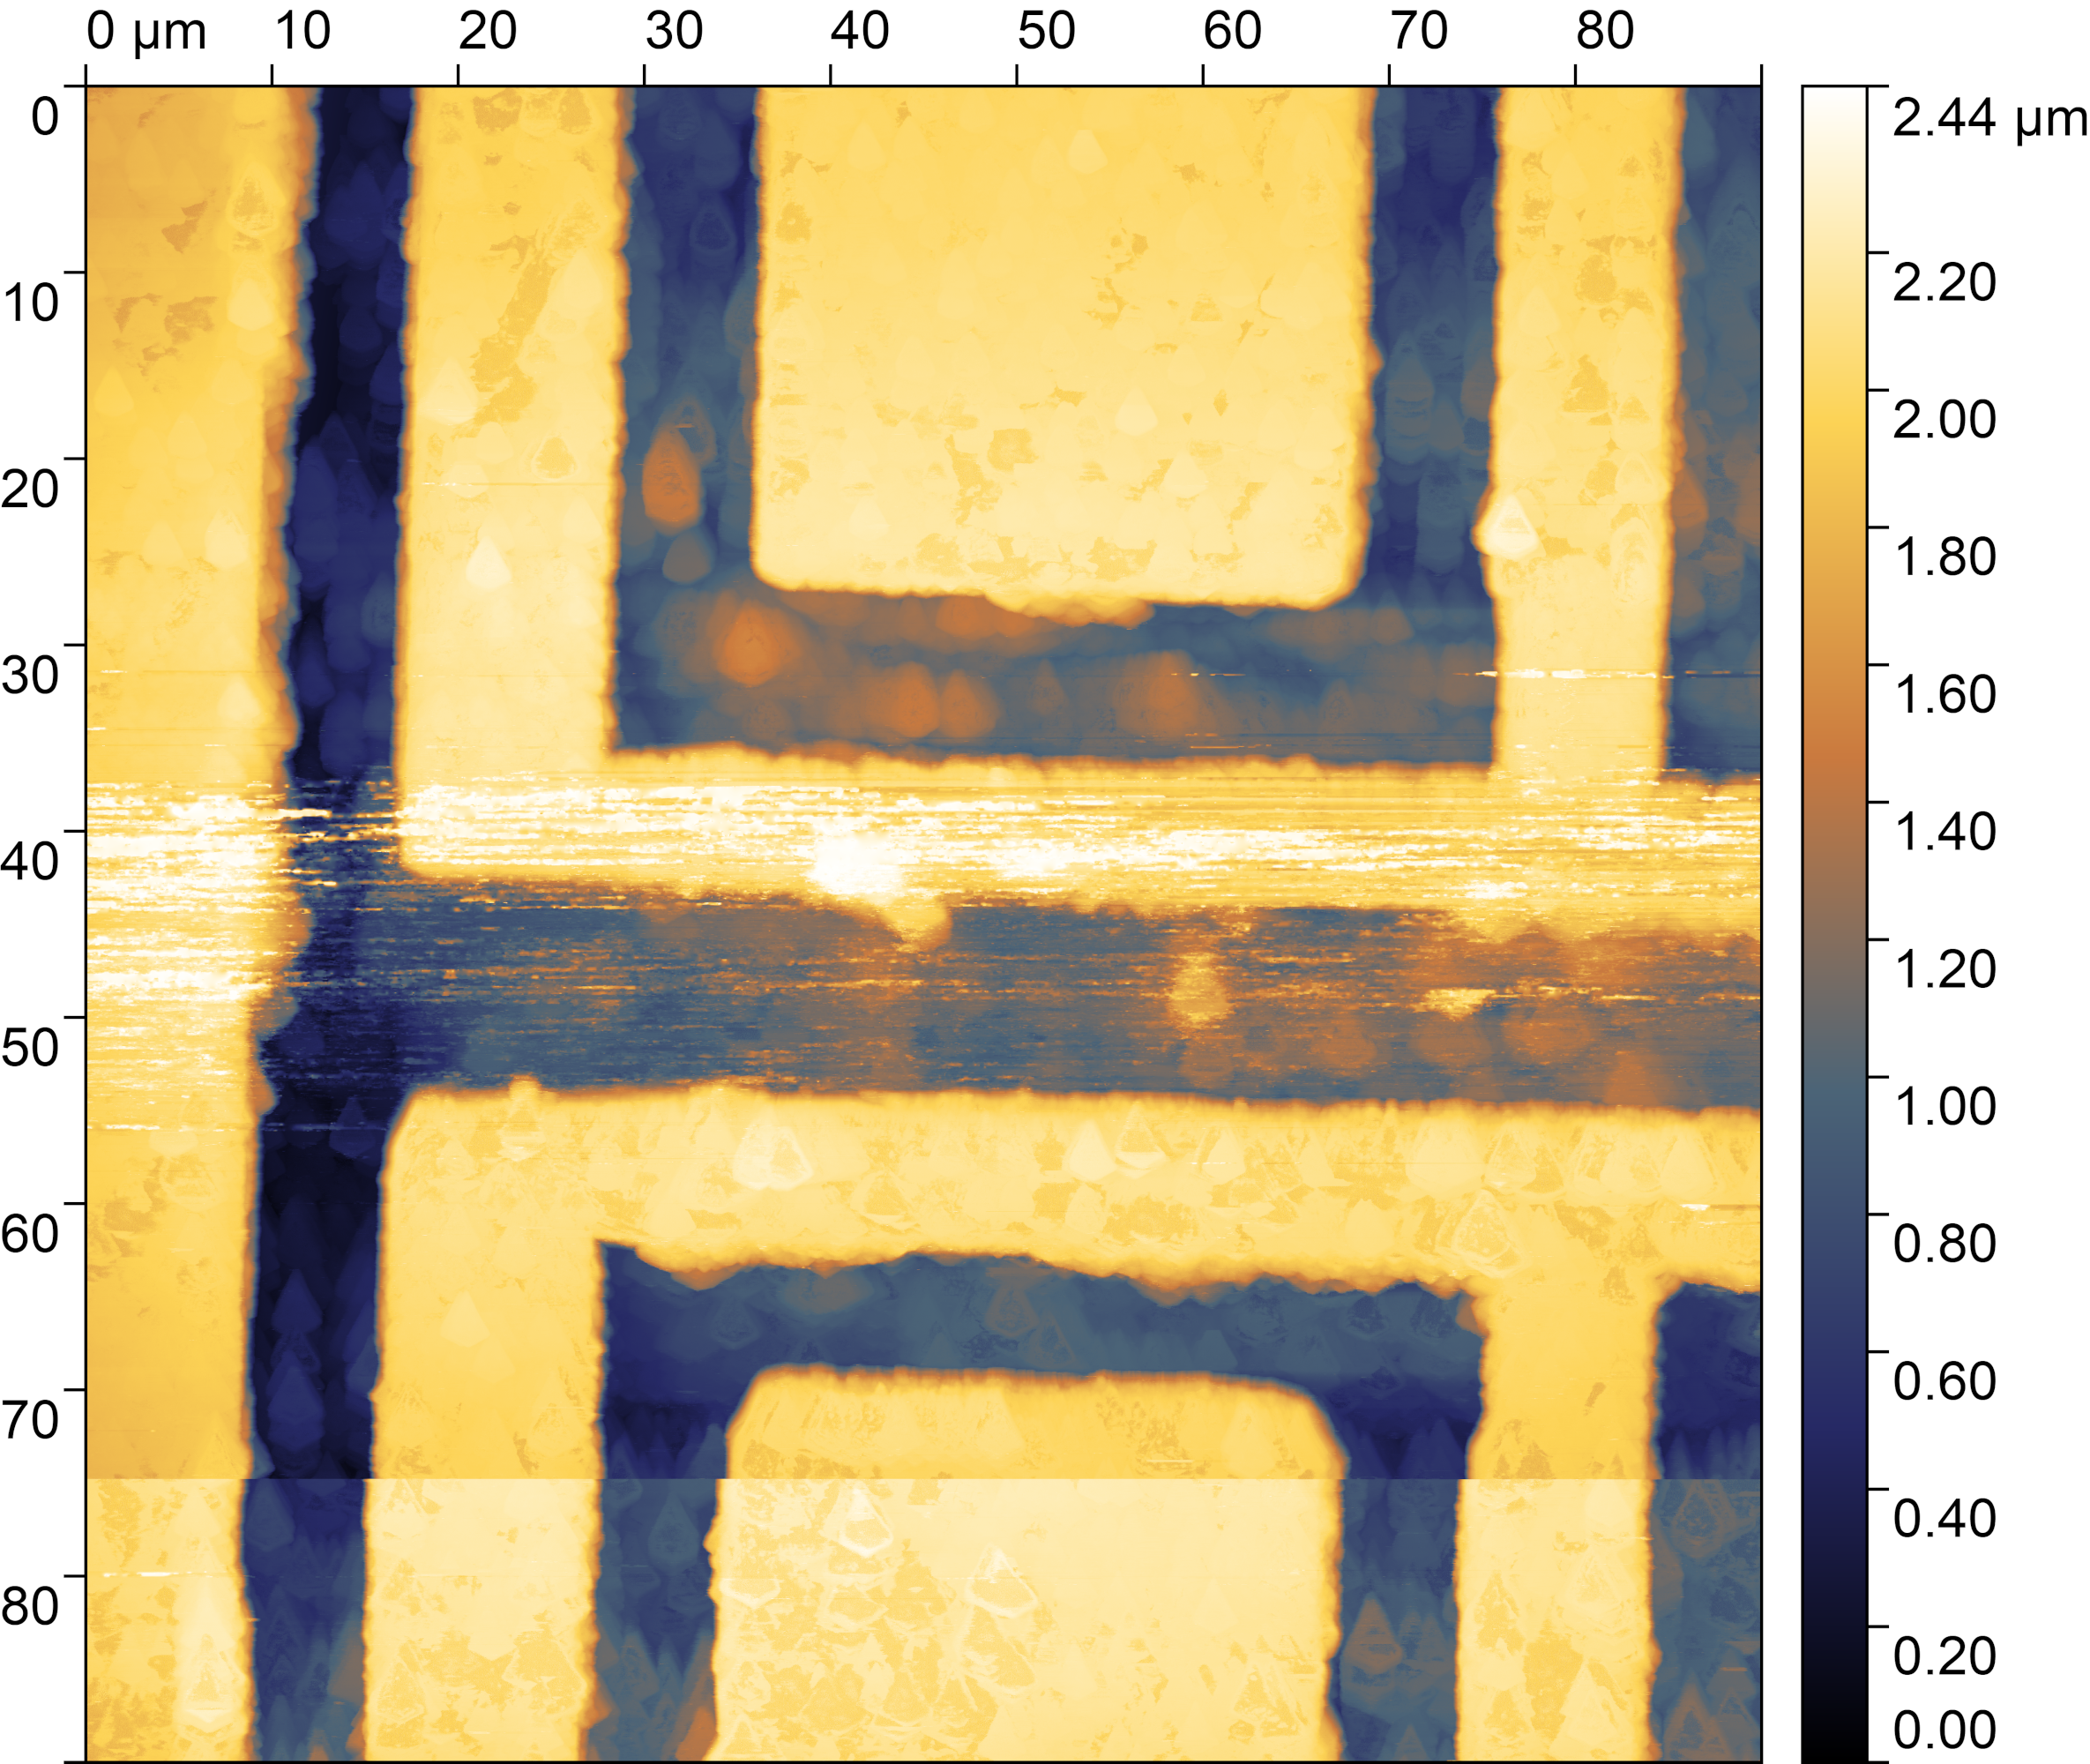
\includegraphics[width=\textwidth]{Chapter7/Figs/Raster/bone_scan_whiteh_downscaled.png}
    \caption{A large area AFM scan of the wider graphitised surface wire, with adjacent contacts for emitter array testing.}
    \label{fig:afm_bone}
\end{figure}

Figure \ref{fig:afm_bone} displays a portion of the control surface wire that was included in the graphitisation design for calibration purposes. This surface wire had a designed thickness of 14~\si{\micro\metre}, to allow for preliminary testing of the written graphite resistivity. While this large scale AFM scan suffers from some noise in the centre of the scan region, it does provide another view of the as written structures, and how they deviate from the design with specific topological features apparent on the sides of the contact wires. The laser written contacts are observed to be up to approximately 2~\si{\micro\metre} deep relative to the diamond surface, with steep walls at the side of the written trenches.

\subsubsection{Trench Wall Steepness and AFM Tip Profile}
\label{subsubsec:trench_wall_steepness}

\begin{wrapfigure}{r}{0.5\textwidth} % 'r' for right, 'l' for left; and the width of the figure.
  \centering
  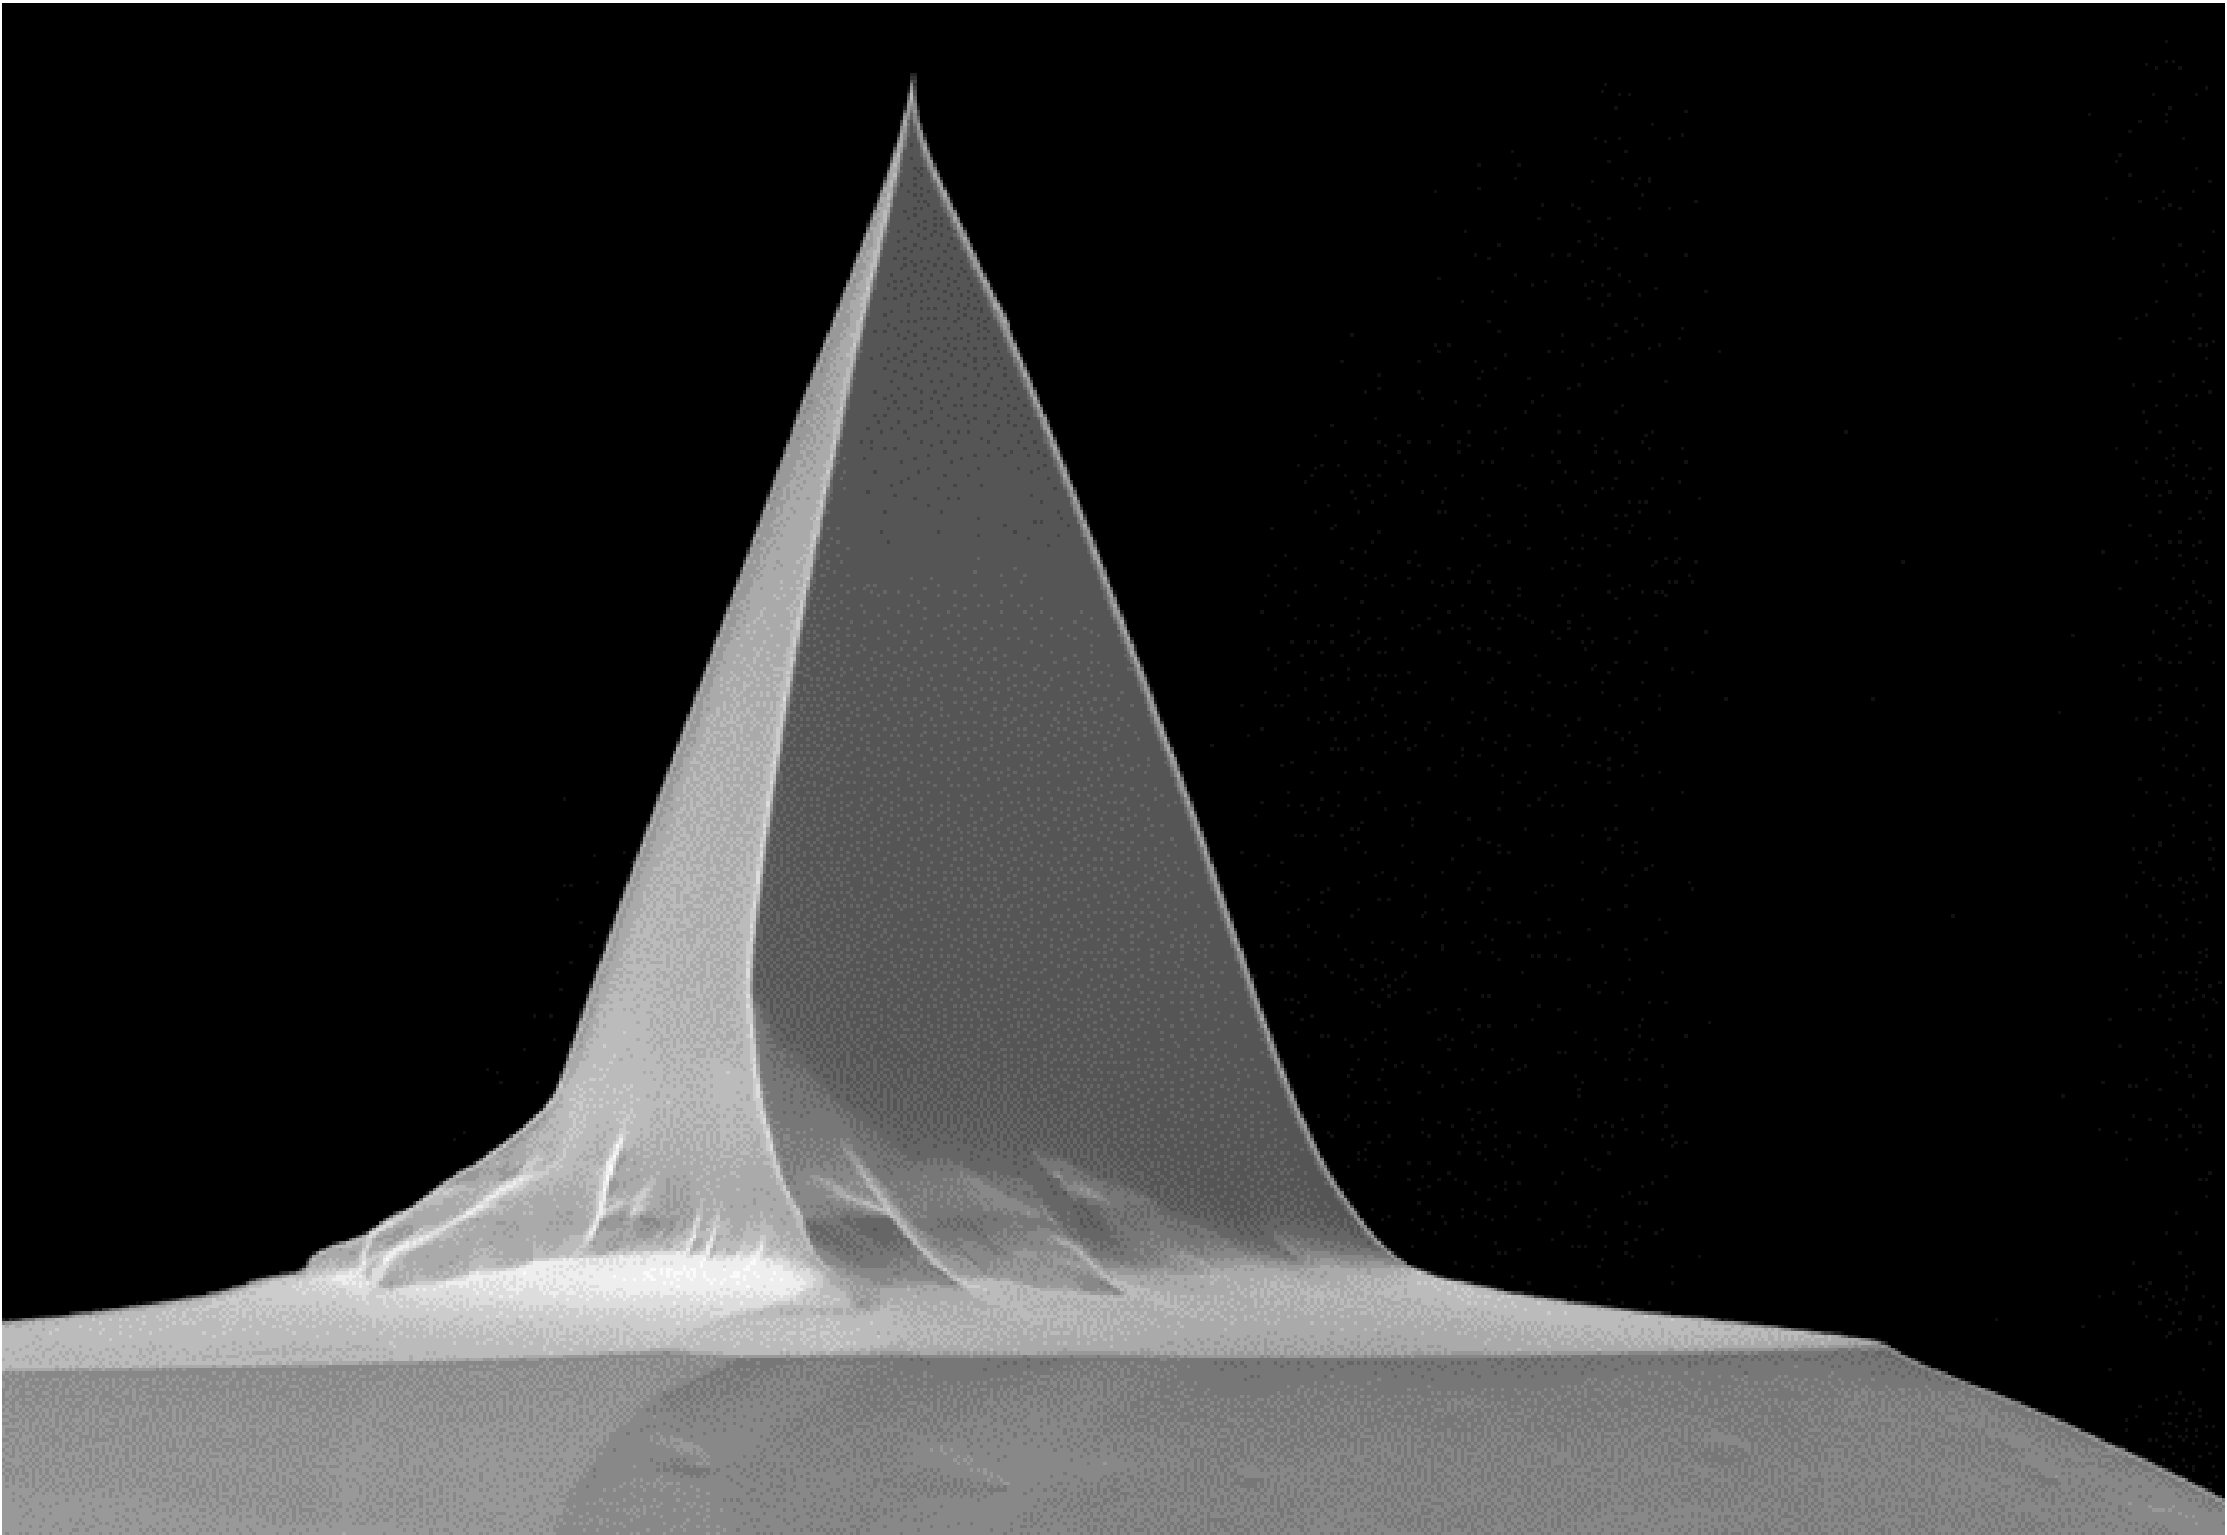
\includegraphics[width=0.48\textwidth]{Chapter7/Figs/Raster/ACTA tip.png}
  \caption{An SEM scan of a typical ACTA tip, as provided in the technical specifications sheet by Applied NanoStructures Inc.}
  \label{fig:acta_tip}
\end{wrapfigure}

It is important to note one detail in particular of the AFM scans, that of the graphitised trench steepness, or the profile of the trench walls. The AFM calibration and background theory is described more fully in section [AFM introduction and calibration section], but for the purpose of examining the large area AFM scans, it is necessary to consider more precisely the observed steepness of the written contacts and the possible impact of the AFM tip itself. Figure \ref{fig:acta_tip} shows a typical ACTA probe as were used in these scans, utilising a rectangular Si cantilever, a pyramidal tip of height $14$--$16$~\si{\micro\metre} and radius of curvature $6$~\si{\micro\metre}. The exact dimensions of the AFM tip may differ from probe to probe, but the pyramidal tip may have had some impact on the observed steepness of etched trenches due to the widening of the base away from the tip.

In NC-AFM, D-AFM or C-AFM, when the tip passes from the diamond surface into the trench, it will quickly descend, with the rate of descent determined primarily by the chosen drive in the Z-scanner. This is then recorded as an incline and less steep wall, with the exact slope being determined by the scan rate if the tip is in relative free-fall after leaving the diamond surface. Equally, when the tip is instead passing from the trench and encounters the trench wall, it may detect the wall itself well beyond the point of the tip coming into contact, due to the pyramidal base meeting the wall first. The piezoelectric system will hence raise the tip, as it detects the side wall with the pyramidal base as for the tip. In this situation, the scan rate may also lead to the risk of direct collision between the pyramidal base and the sidewall, ultimately leading to damage of the AFM tip.

\begin{figure}[H]
    \centering
    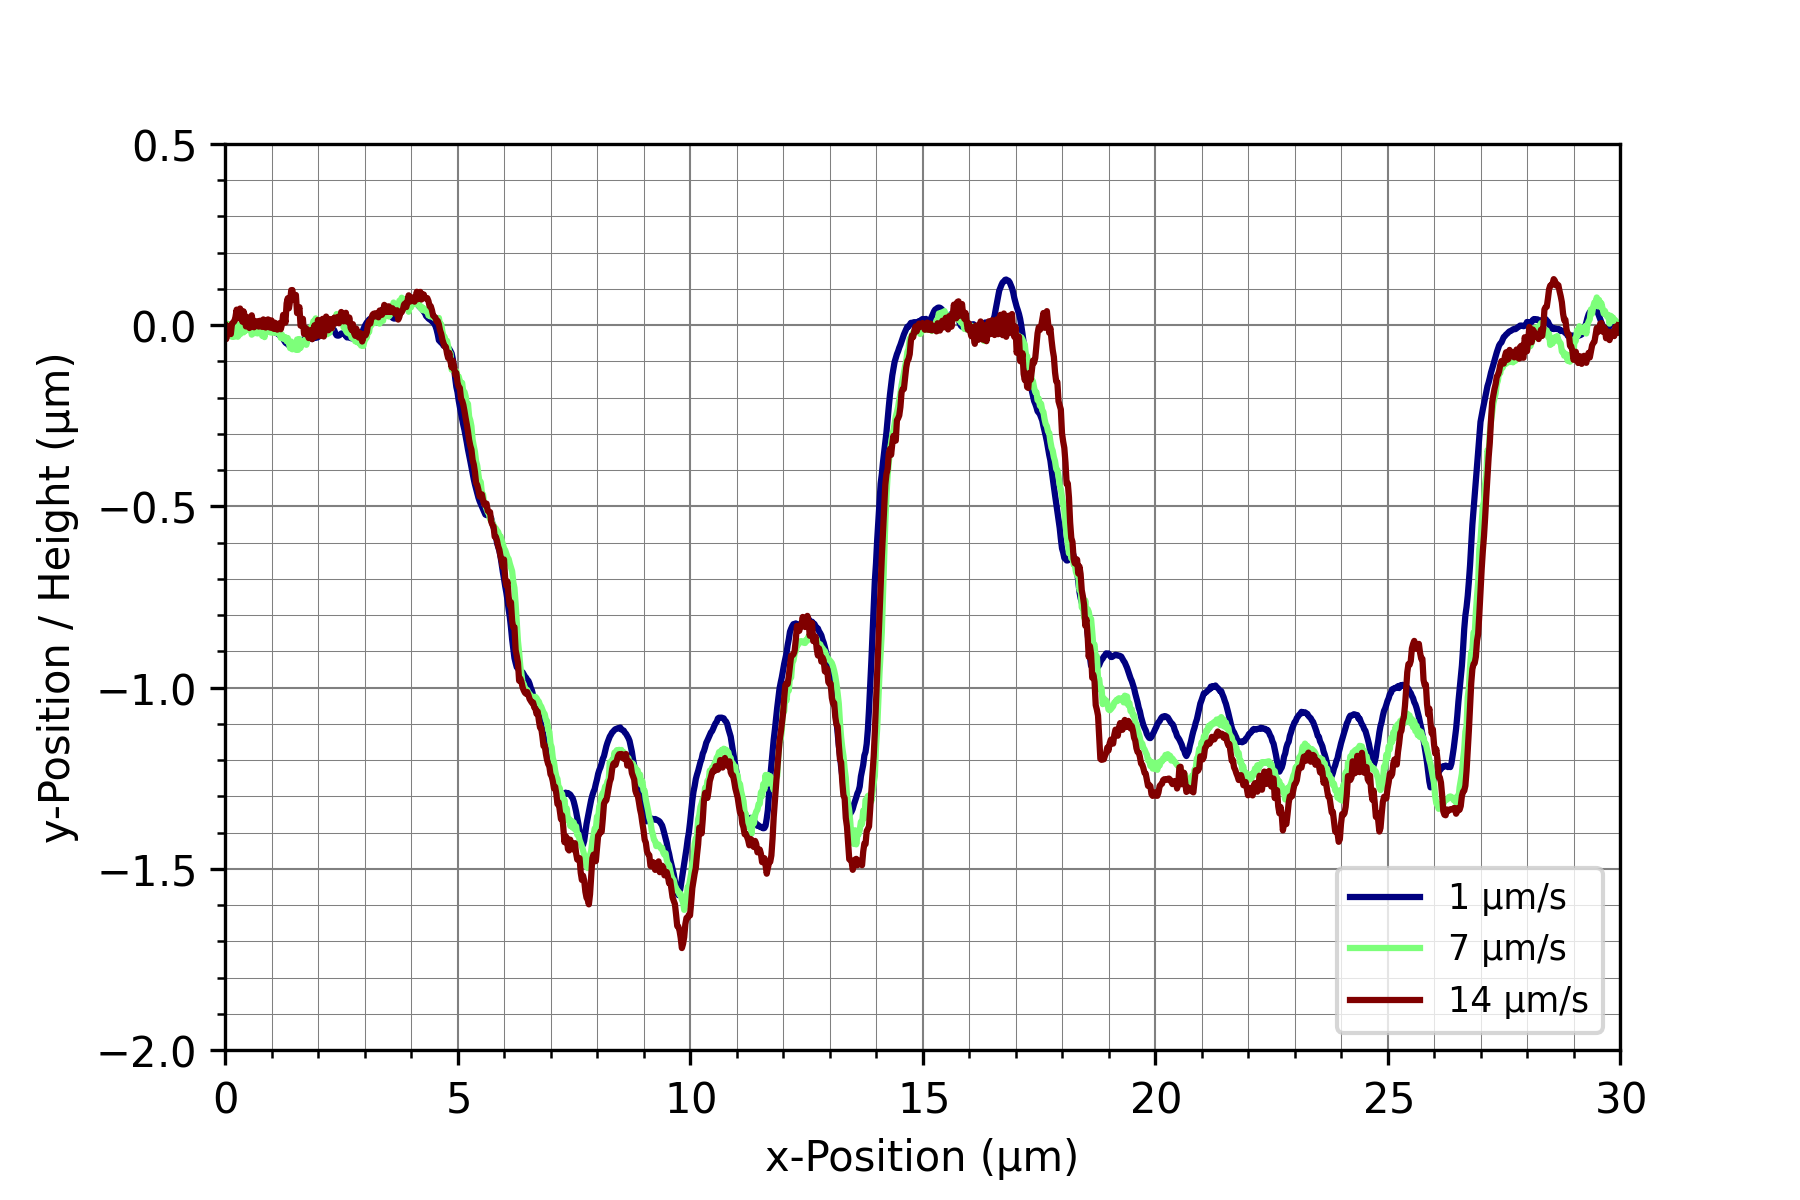
\includegraphics[width=\textwidth]{Chapter7/Figs/Raster/jet_legend_um.png}
    \caption{A comparison of three different NC-AFM scan rates on a laser graphitised trench structure. The data are planarised based on the first and last data points, to represent the estimated diamond surface level.}
    \label{fig:afm_scan_rate_small}
\end{figure}

Figure \ref{fig:afm_scan_rate_small} has a few notable features which demonstrate this process when using NC-AFM. First, all three scan rates have distinct peaks and troughs as they pass through the laser graphitised channels. The sharp, triangular troughs perhaps directly reflect the triangular AFM tip in action when it meets a sharp drop in the z-axis. Second, it is clear that the direction of the scan impacts the observed edges of the graphitised trenches. In this figure, the scan is passing from the left to the right. While the first trench appears to have a relatively low slope, with agreement between all three scan rates, the descent into the second trench has a notable discrepancy between the two lower scan rates and the highest included scan rate of $15$~\si{\micro\metre\per\second}. In contrast, the walls as seen by the ascending AFM tip are in relative agreement, as they all encounter the wall and must ascend very quickly to ensure that the tip does not impact the wall. It is also notable that the observed trench depth decreases as a function of the AFM scan rate, indicating that at the lowest scan rates the system is better recognising the correct altitude of the tip, as it has time to adjust based on the specific features within the channels.

\subsubsection{Further AFM Scans}
\label{subsubsec:further_afm_scans}

\begin{figure}[H]
    \centering
    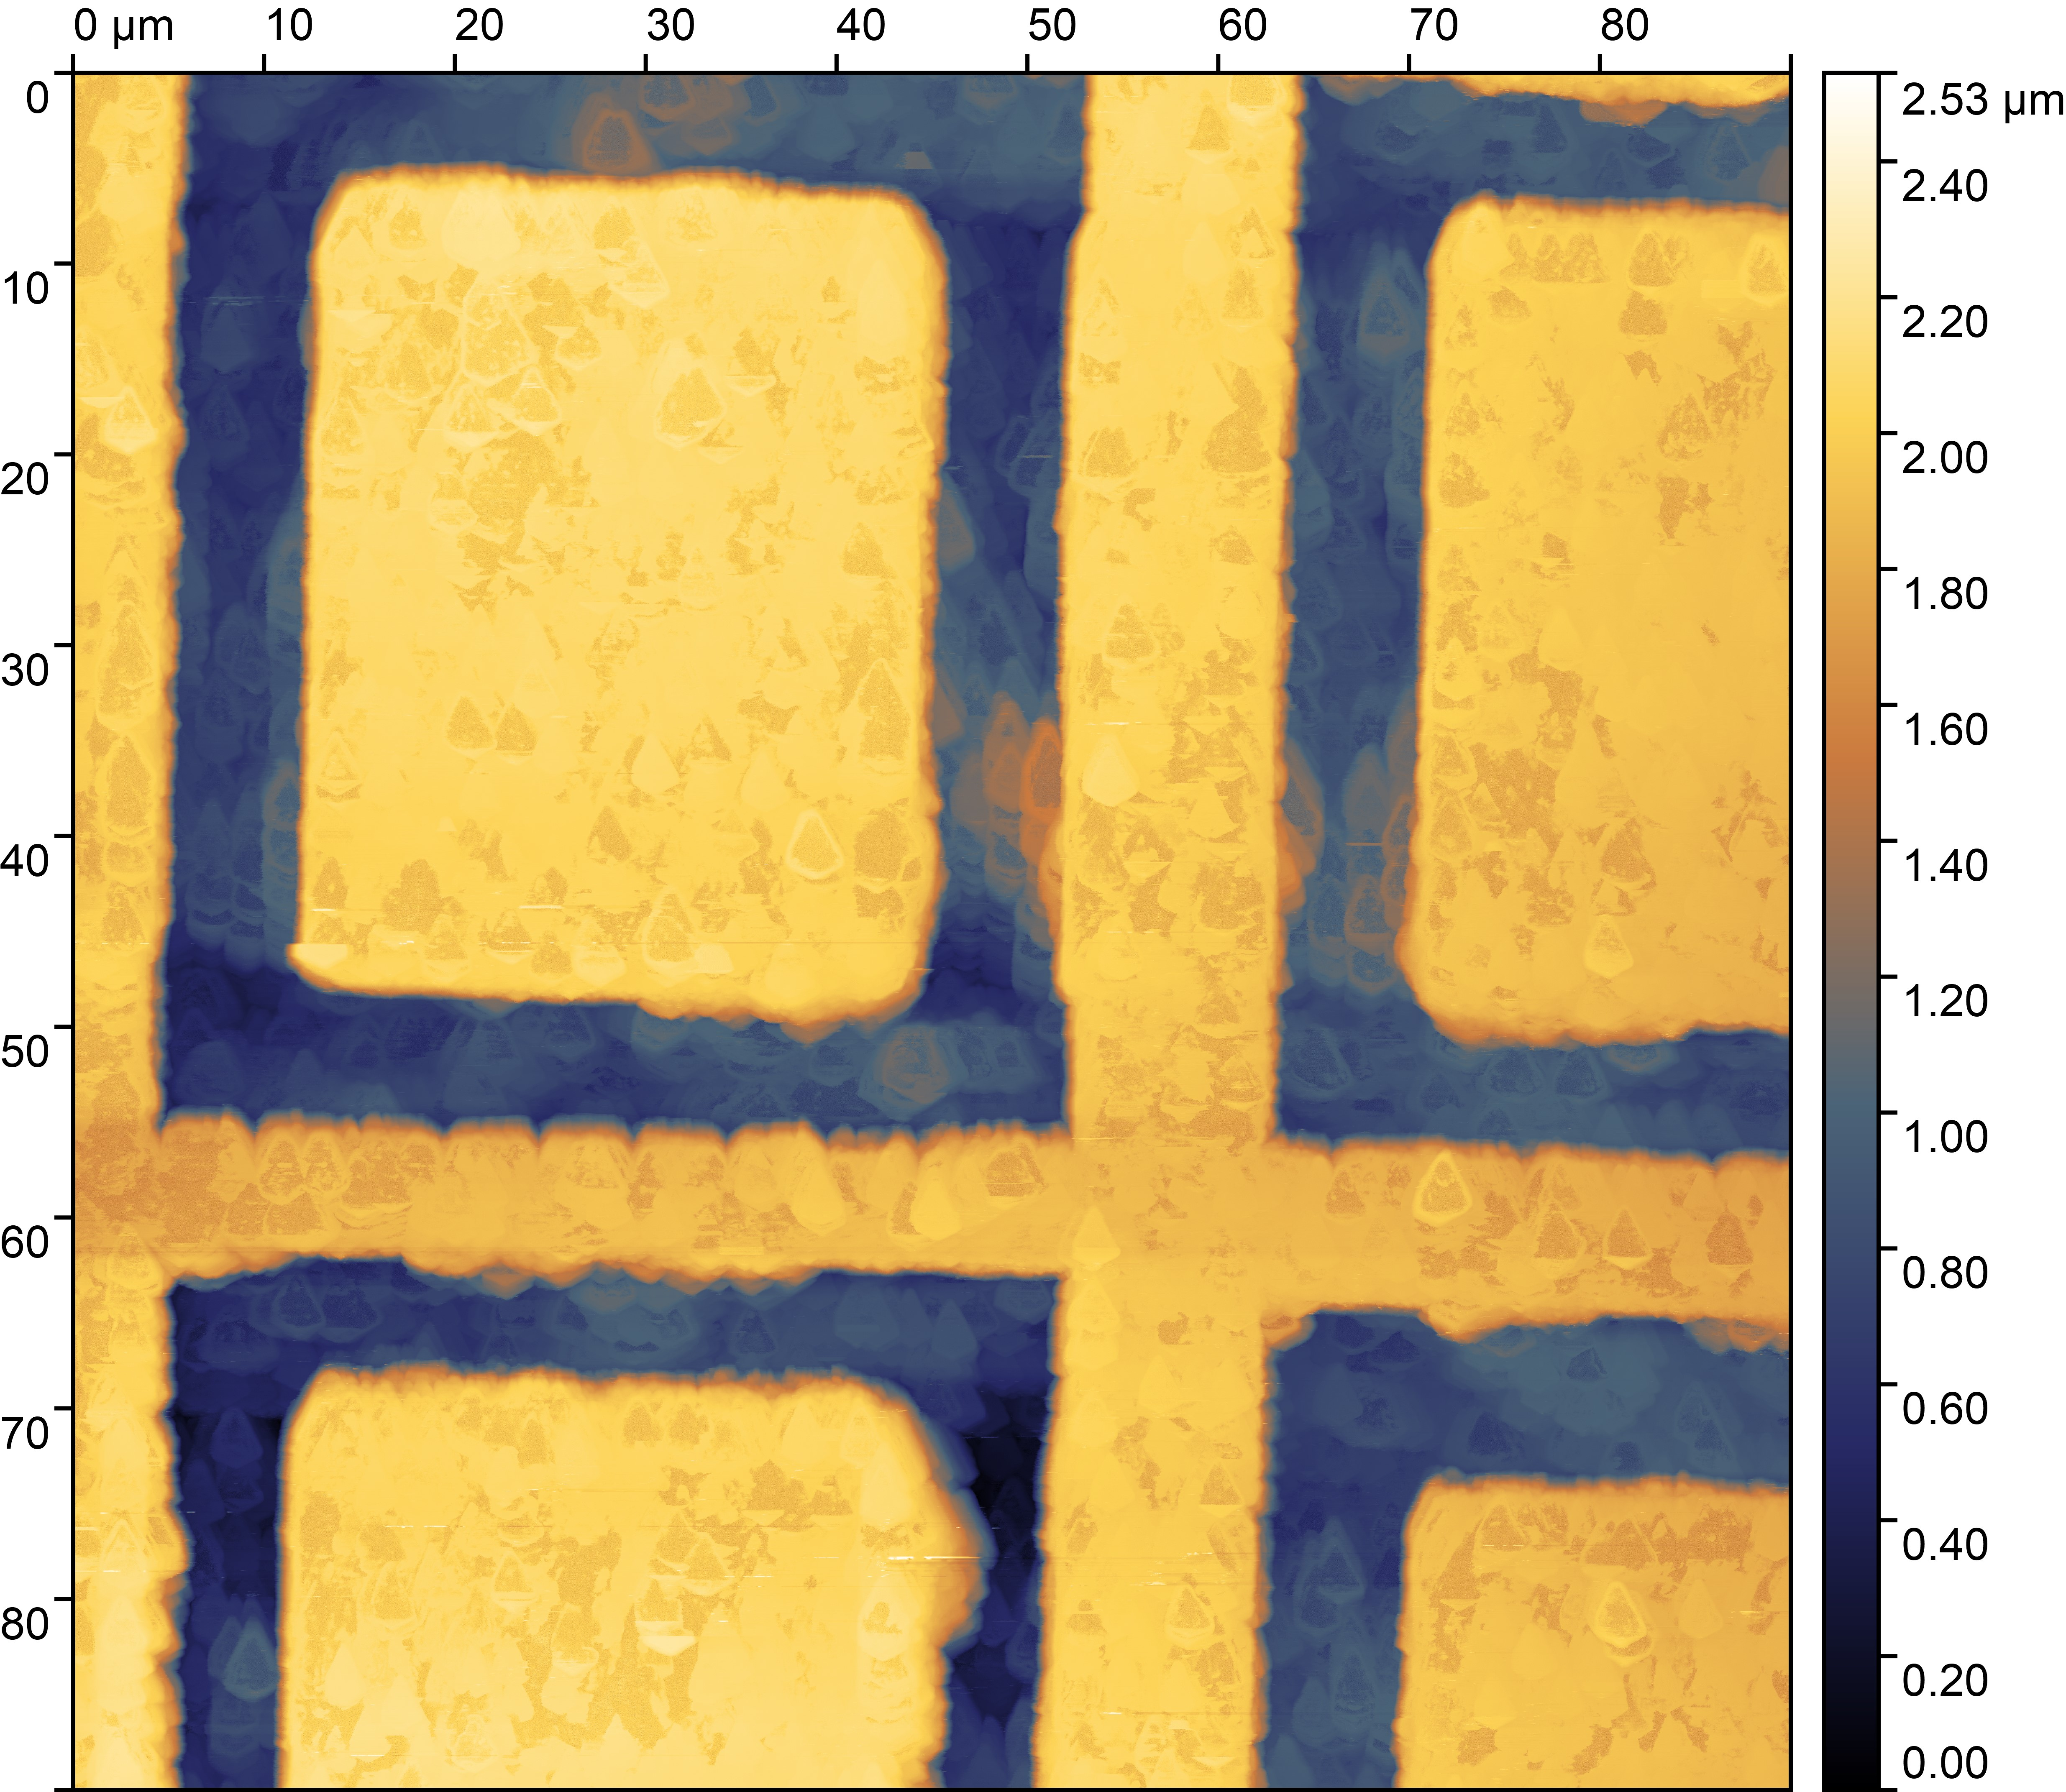
\includegraphics[width=\textwidth]{Chapter7/Figs/Raster/AF emitter array afm.png}
    \caption{A large area AFM scan of emitter array AF that was used for electrical characterisation.}
    \label{fig:afm_af_large}
\end{figure}

Figure \ref{fig:afm_af_large} shows a large area AFM scan that was taken to examine the effective topology of an emitter array type structure as written via laser graphitisation. In this figure, almost the entirety of contact A (top left) is visible, with contact F directly below (bottom left). In-between these two contacts, extending downwards from contact A, the beginnings of the laser written wire structures are just about visible as depressions in the topology. This also provides another general view of the laser writing process and the sometimes inconsistent structures that are written on the diamond surface. In some places, there are very noticeable protrusions into the otherwise rectangular contact structures. As this is purely a topological scan, this hence displays a lack of ablation in these regions, perhaps due to a lack of graphitisation processes, lower laser absorption, or other changes in the writing process. Similarly, some areas within the contact structures appear to have a greater depth than the majority of written area, perhaps due to a greater absorption of laser power in these specific regions, or perhaps more readily graphitised and subsequently ablated diamond.

\begin{figure}[H]
    \centering
    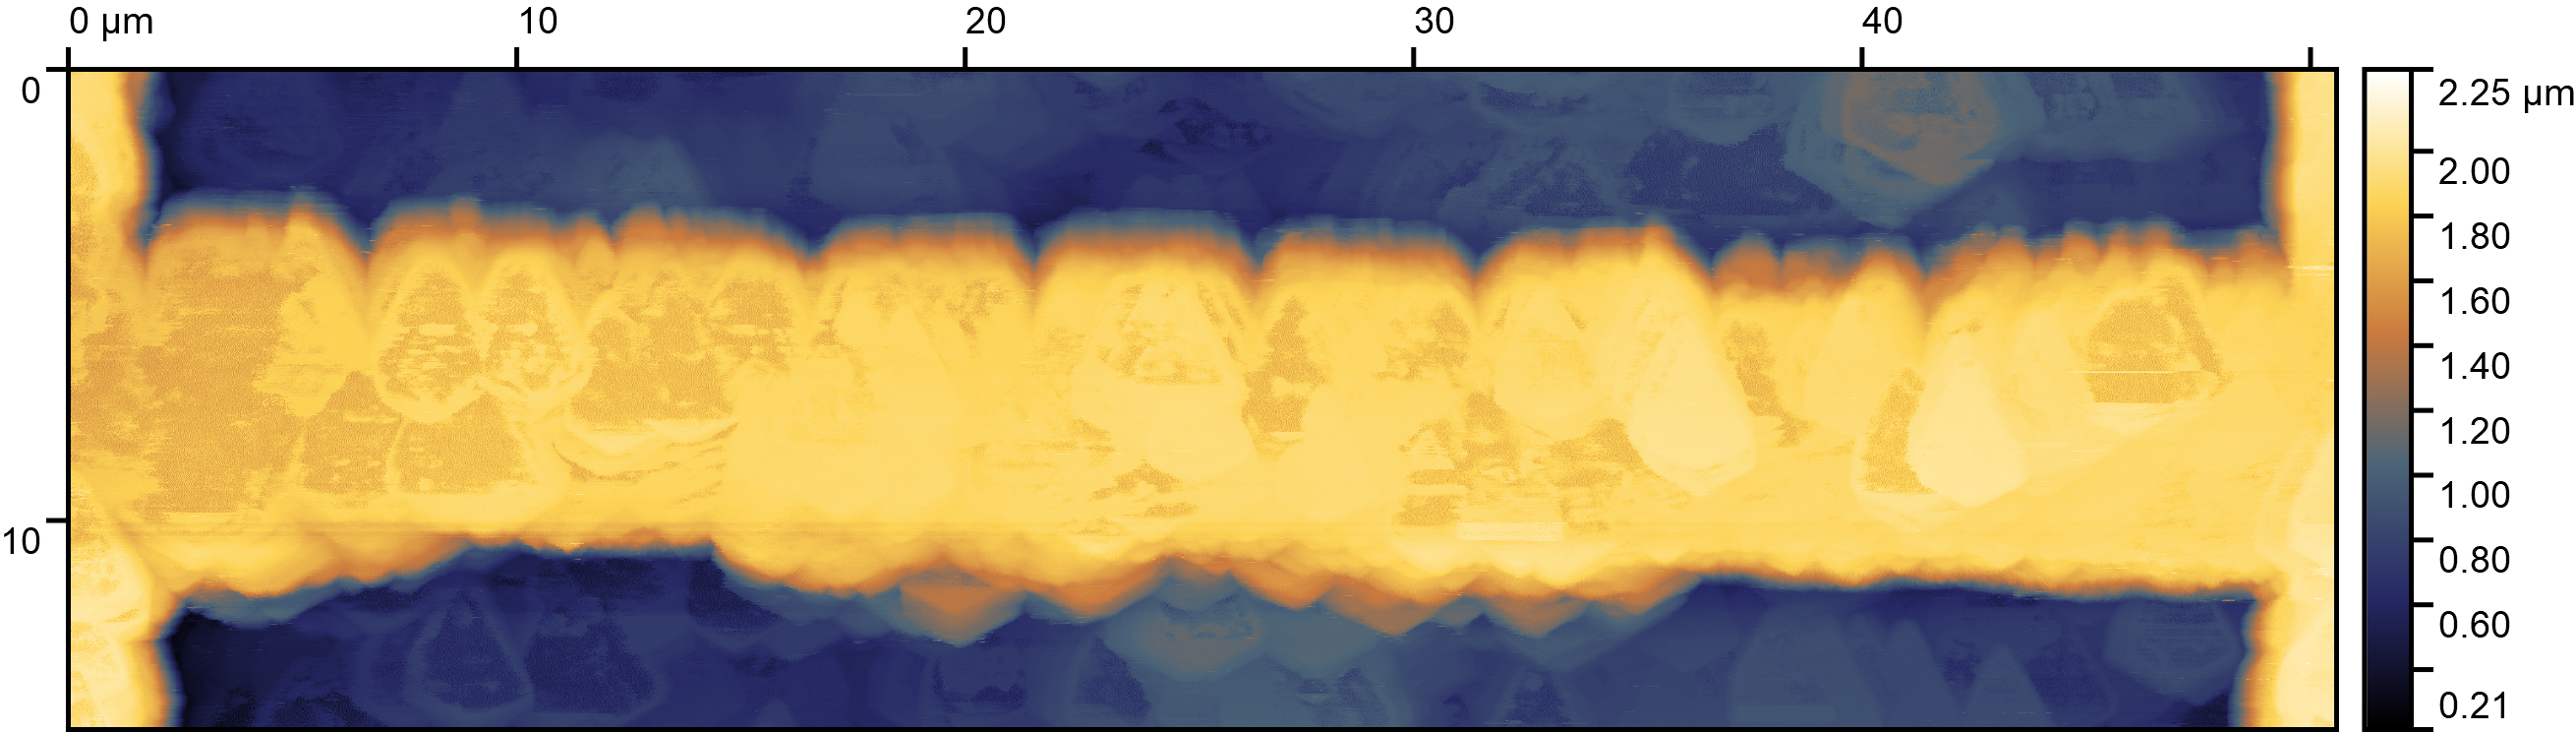
\includegraphics[width=\textwidth]{Chapter7/Figs/Raster/af_cropped_emitters.png}
    \caption{A cropped AFM scan of emitter array AF that was used for electrical characterisation.}
    \label{fig:afm_af_crop}
\end{figure}

\begin{figure}[H]
    \centering
    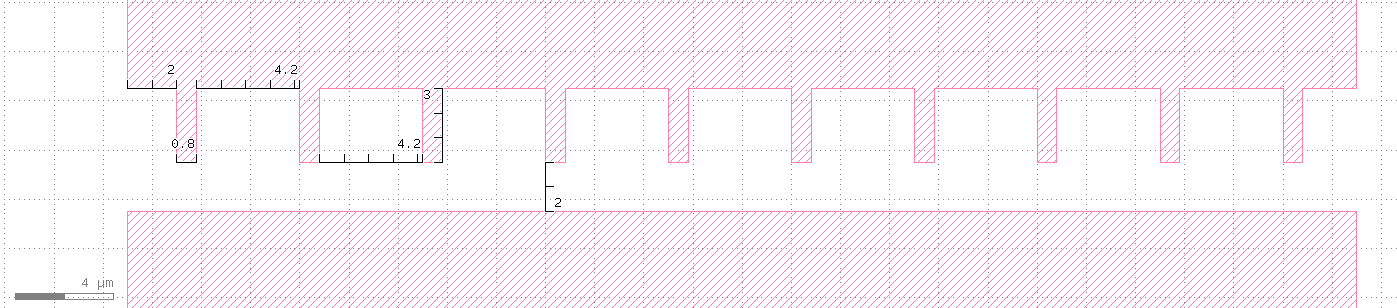
\includegraphics[width=0.95\textwidth]{Chapter7/Figs/Raster/af_emitter_design1.png}
    \caption{A cropped view of the AF emitter array design, with feature size measurements provided.}
    \label{fig:afm_af_design}
\end{figure}

For clarity, the region between contacts A (upper) and F (lower) is cropped down and expanded in figure \ref{fig:afm_af_crop}. When compared directly with the designed array in figure \ref{fig:afm_af_design}, the topology does not directly reveal the presence of 0.8~\si{\micro\metre} width emitter wires extending down towards contact F. However it is possible to see what may be the very start of all but the two outer emitter wires, with notable triangular depressions extending nearly as deep as the larger width contact structures.

\begin{figure}[H]
    \centering
    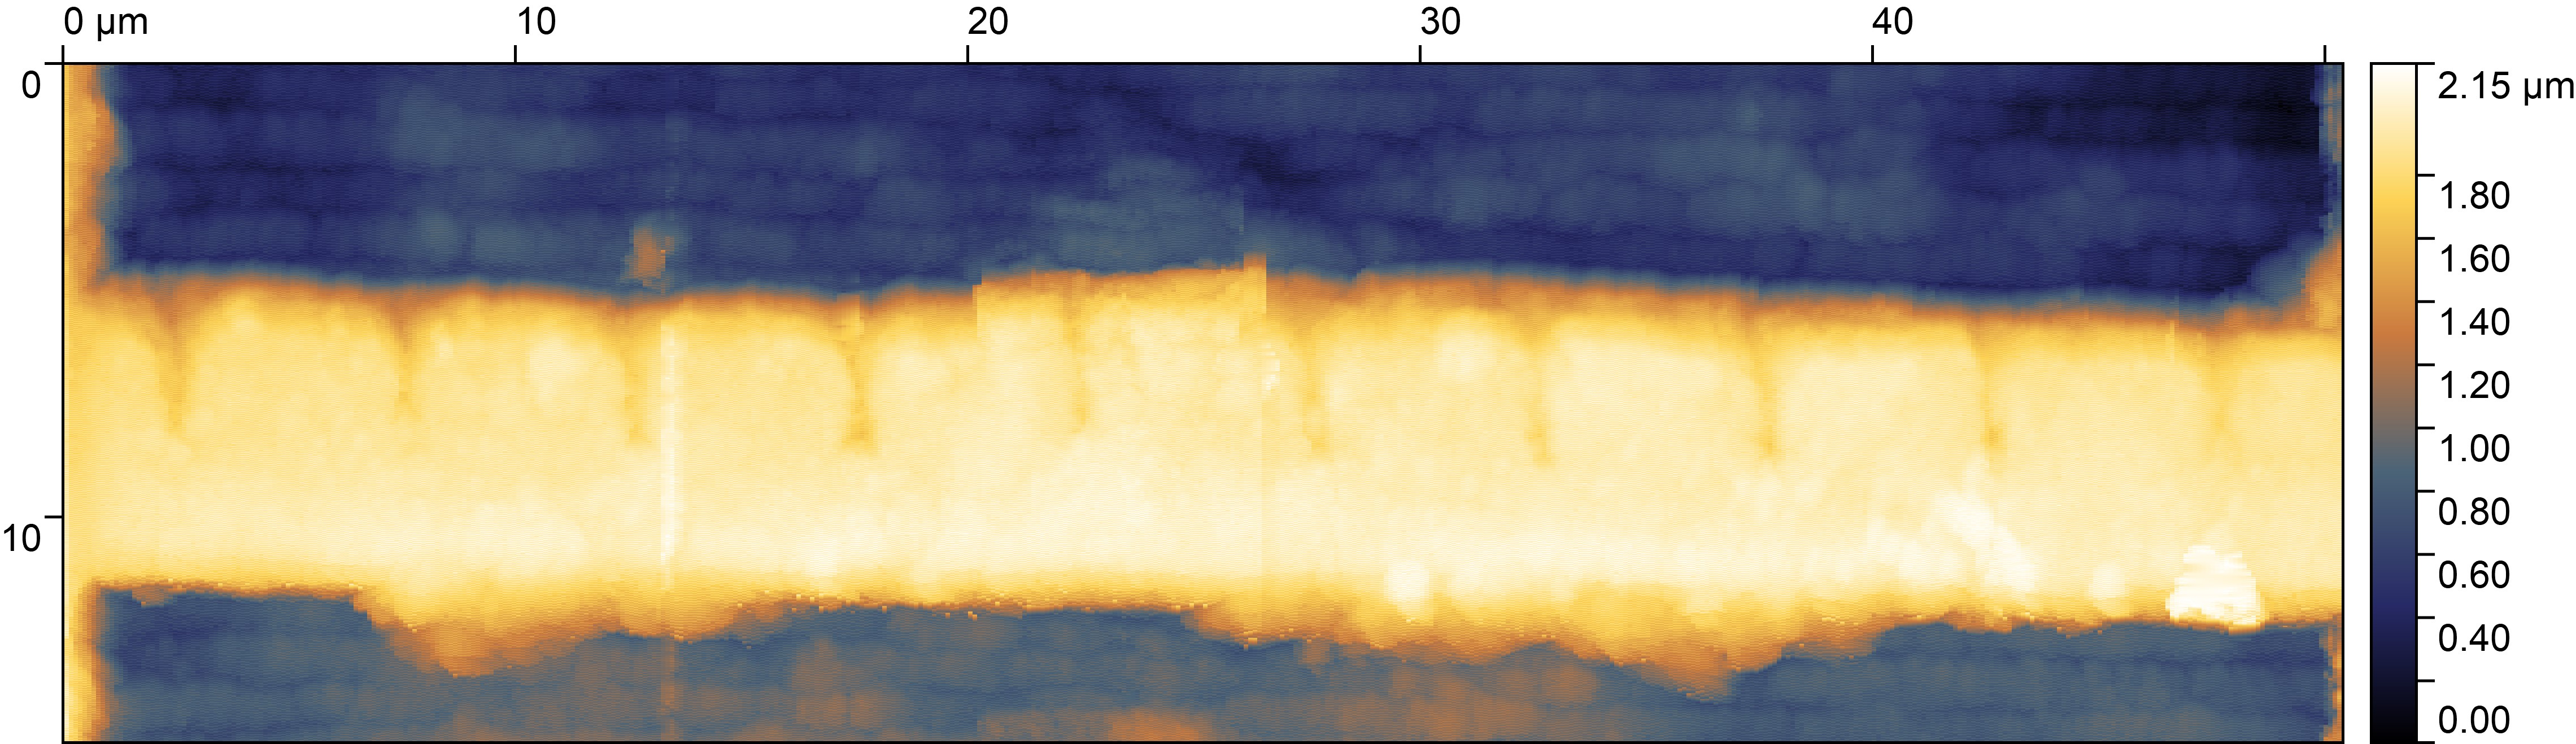
\includegraphics[width=\textwidth]{Chapter7/Figs/Raster/CH_cropped.jpg}
    \caption{A cropped AFM scan of the CH emitter array, with scan direction parallel to the emitter wires (y-axis).}
    \label{fig:afm_ch_array}
\end{figure}

Figure \ref{fig:afm_ch_array} shows another of the emitter array structures that were fabricated on the diamond surface. In contrast to the unclear topology observed with array AF, array CH appears to clearly demonstrate the presence of ablated diamond, and hence the fabrication of emitter wires leading down from contact C into the channel towards contact H. As observed in the wider AFM scans, the intended rectangular contact design for contact H in particular displays some deformation, with notable incongruities along the top of the graphitised region. The success of this AFM scan in displaying topographical results may be attributed to the y-axis scan direction, which is the fast direction. Based on the general observation from scan rate testing that higher scan rates will tend to show a lower slope of descent, and a higher angle of ascent, one clear practical approach to accurately detecting sub-micron thickness graphitised wires is to scan along the length of the emitter, rather than across the width. This ensures that the tip does not need to descend into the emitter channel, and instead as it passes down from the contact region, it will tend to only require a raised elevation as it progresses. When running in the reverse direction (up from contact H), again only one clear descent is necessary to enter the emitter channel, where the tip then remains as it passes down the channel. Hence, the slow scan rate direction is then across the width of the emitters, and is best able to detect any change in topology. A further detail with this approach is that this requires a suitable pixel density, as the number of pixels across the width of the emitter channel directly translates to the number of points along the length of the emitter where the tip will travel, measuring the depth of ablated material. Hence, in this example with a fast scan rate of 7.5~\si{\micro\metre\per\second} and a raw scan size of 62~\si{\micro\metre} x 15~\si{\micro\metre}, to observe emitter widths of 0.8~\si{\micro\metre}, the effective pixel width must be below 0.4~\si{\micro\metre} to ensure that the AFM tip does indeed enter the graphitised emitter channel, in a near central location. For this scan a pixel width of $\sim0.24$~\si{\micro\metre} appears to have been sufficient to positively identify ablation related to the formation of graphitised emitters, especially combined with the slow scan rate direction and the top-down AFM tip pass scan direction.

The design of emitter array CH was otherwise very similar to AF, with 10 emitter cathodes of width 0.8~\si{\micro\metre} spaced 4.2~\si{\micro\metre} apart across the 60~\si{\micro\metre} contact structure (C). The only difference was in the cathode-anode spacing, due to a slight shortening of the emitter wire, which in the case of AF was 2~\si{\micro\metre}, and for CH was 2.5~\si{\micro\metre}. Preliminary low resolution AFM scans indicated that array CH was one of the clearest examples of the intended emitter structure, and so this was selected for electrical characterisation alongside AF.

\subsection{Fluorescence Characterisation}
\label{subsec:fluorescence_characterisation}

\begin{figure}[H]
    \centering
    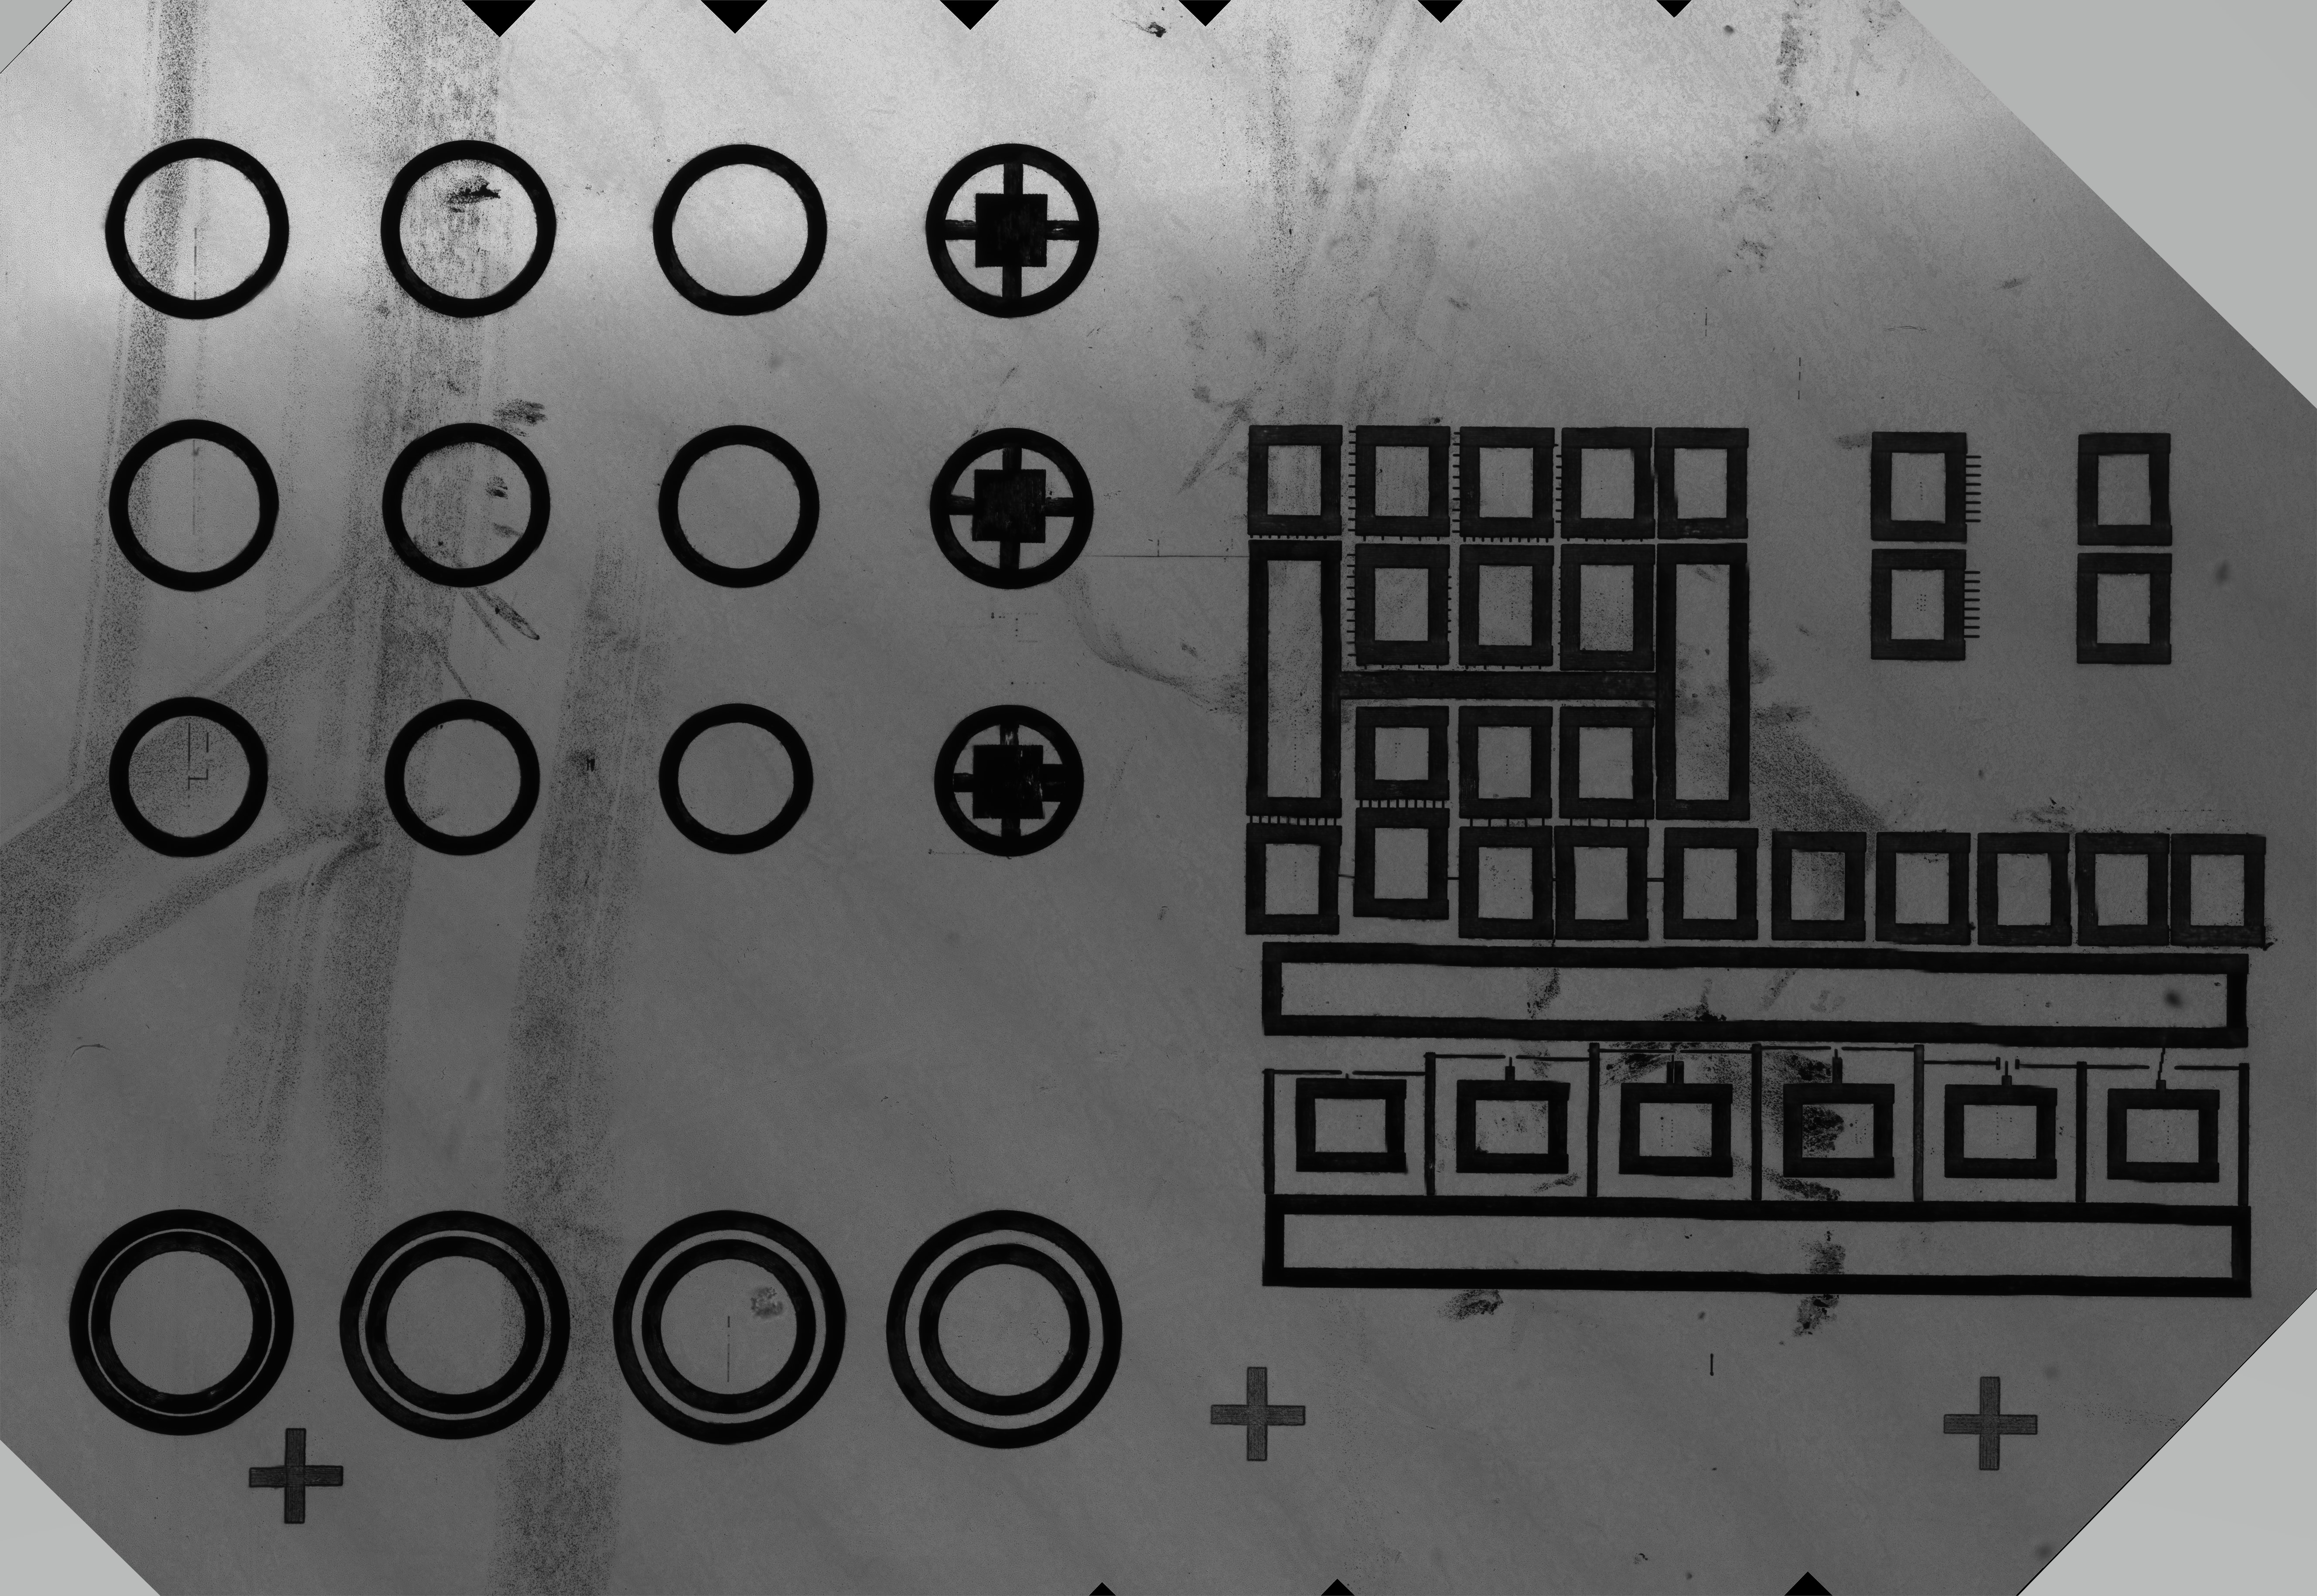
\includegraphics[width=\textwidth]{Chapter7/Figs/Raster/ESID_rotated_downscaled_further.png}
    \caption{An overview of the laser graphitised structure as seen using a backlit 488~\si{\nano\metre} light source and mapping with a confocal microscope.}
    \label{fig:bio_esid}
\end{figure}

One possible source of material characterisation is that of fluorescence. Figure \ref{fig:bio_esid} shows the optical overview provided by the Zeiss LSM 800 system, providing a grouped map of confocal scans that allows for near-diffraction-limited imaging across the entirety of the laser-written structures. The images provided by this system allow for good optical comparisons with the topological AFM measurements, with the change in observed 488~\si{\nano\metre} absorbance due to the graphitisation or amorphisation of carbon perhaps providing a more reliable picture of how well the fabrication of the thinnest laser treated features have formed. Further to this, diamond fluorescence centres offer a unique examination of the composition of diamond defects. In particular, it should be expected that HPHT samples such as those used for the substrates in the current work will have a large concentration of singly substitutional nitrogen, aka C-centres. This imparts the deep yellow-orange colour as is typical for HPHT samples when seen by the naked eye, and is a substantial factor in the characteristic fluorescence of HPHT grown diamonds. 

\begin{figure}[H]
    \centering
    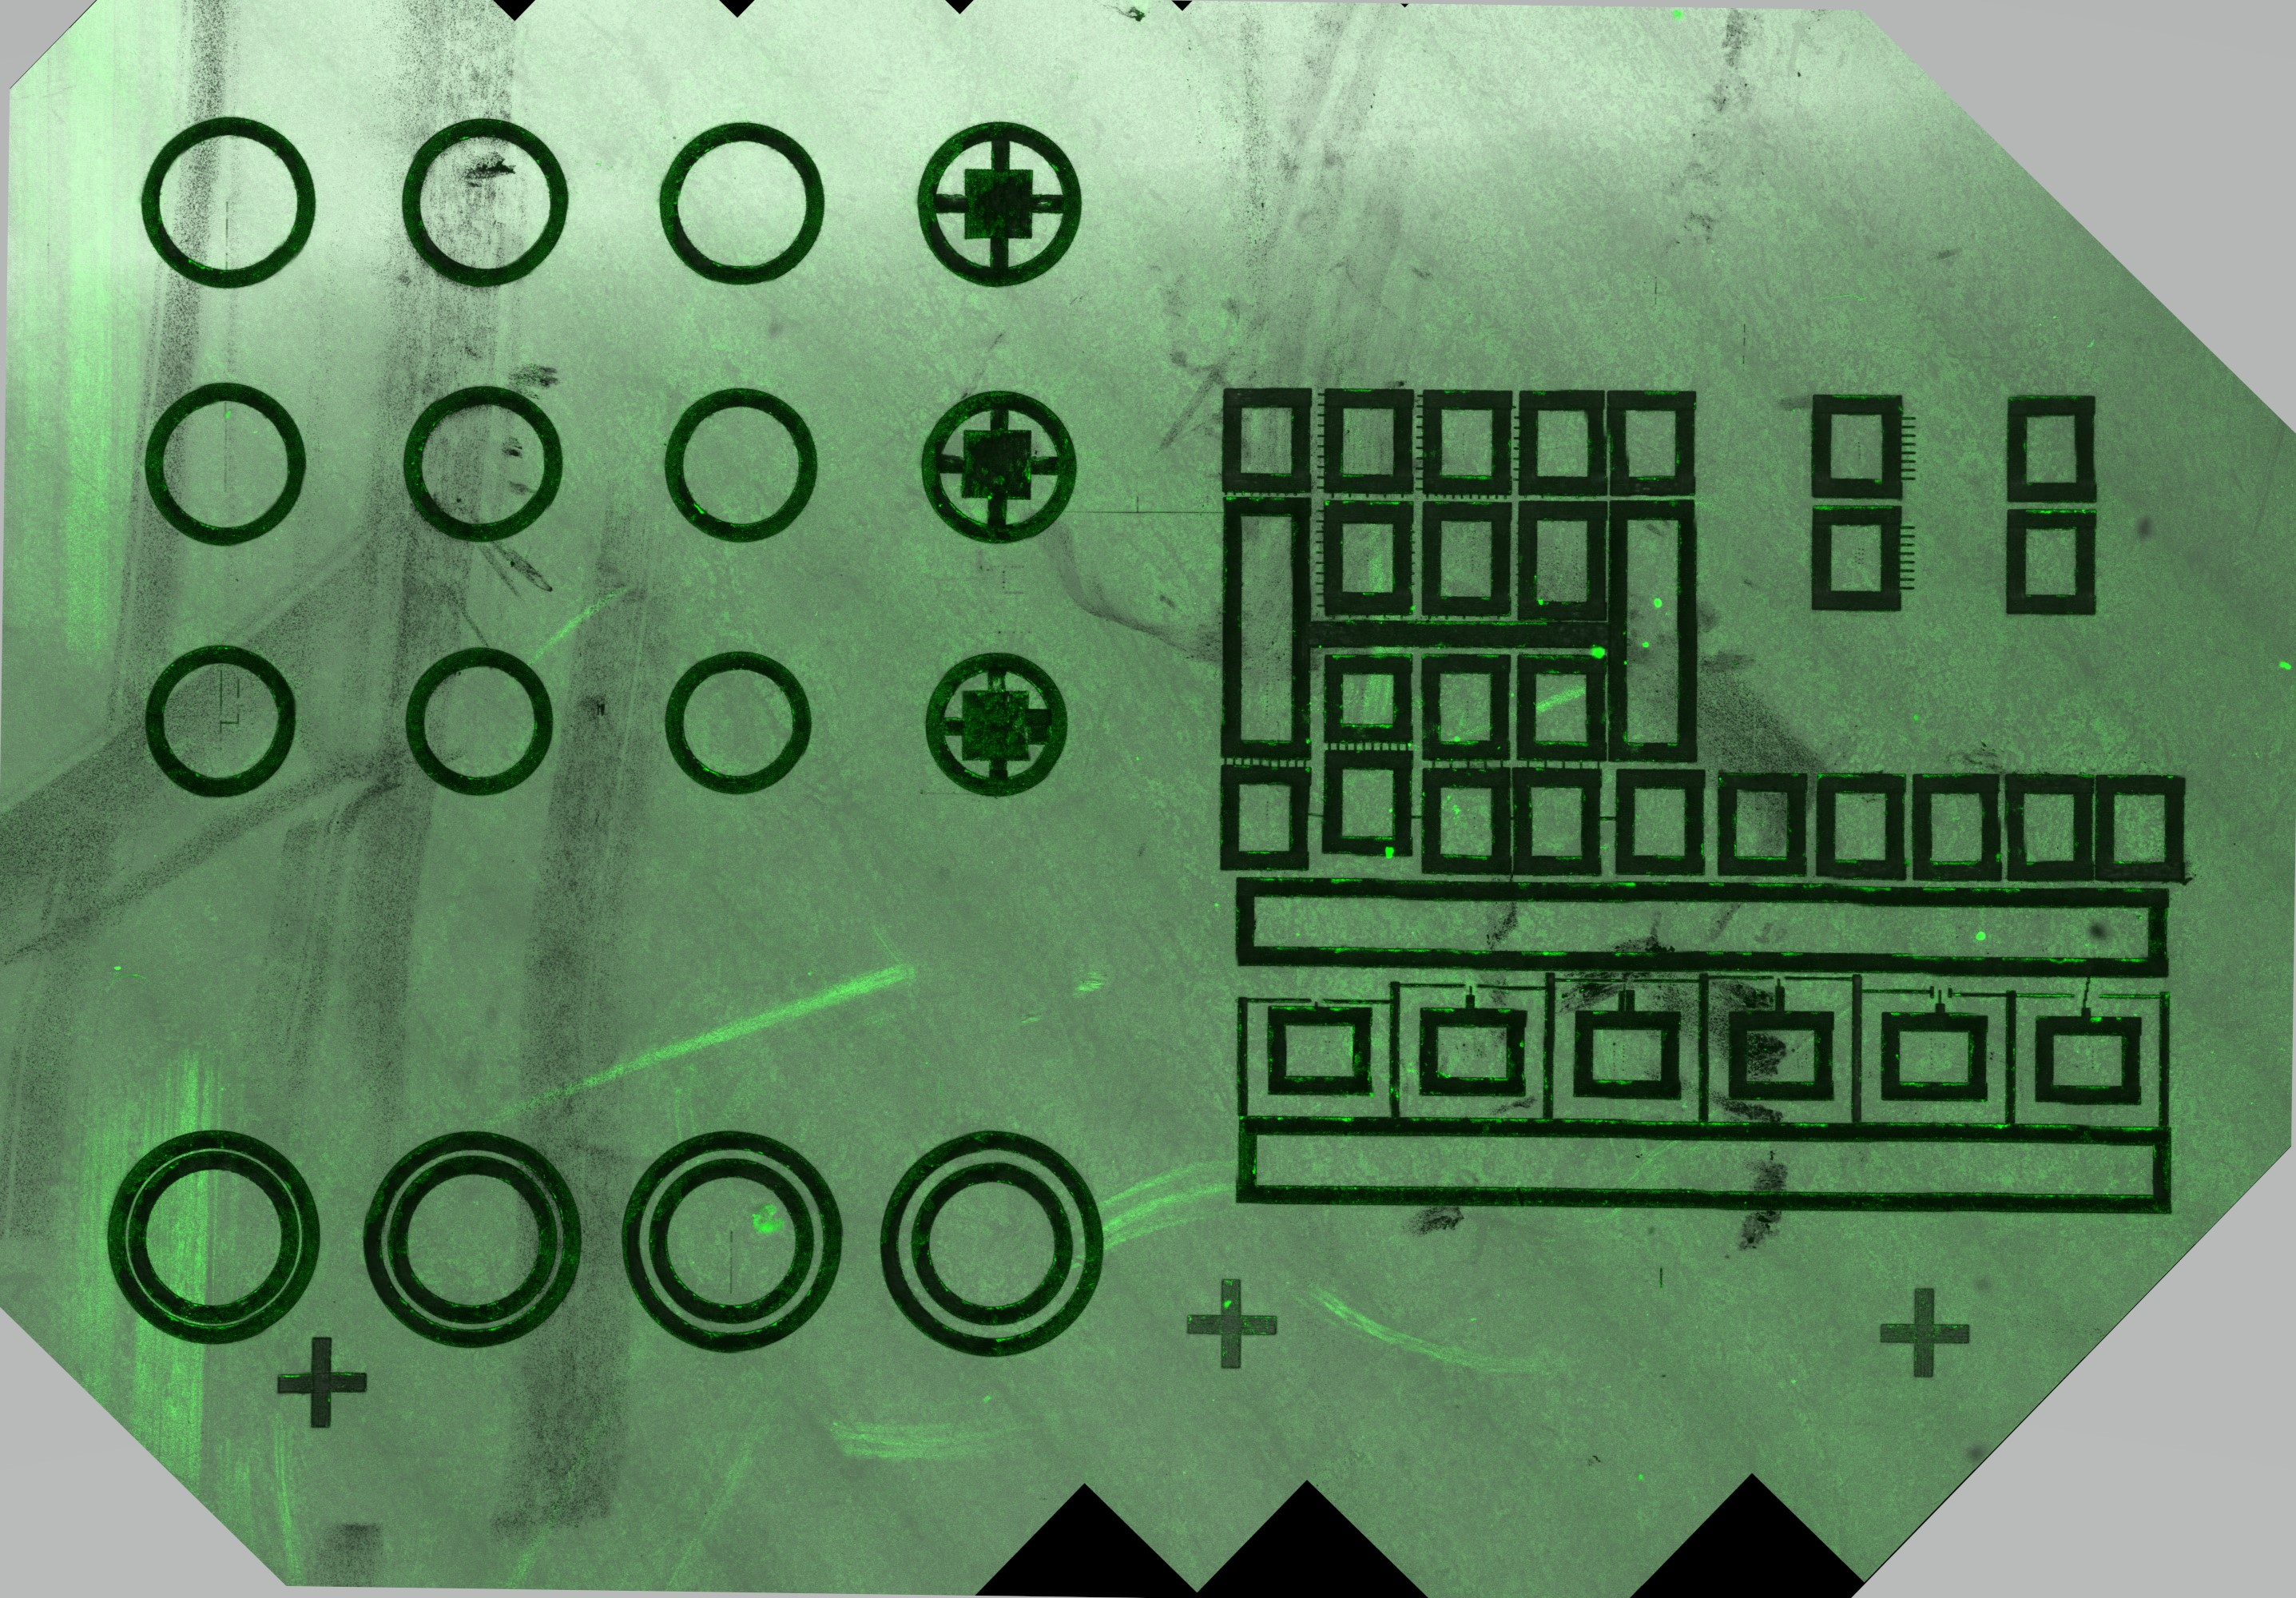
\includegraphics[width=\textwidth]{Chapter7/Figs/Raster/FL_overview.png}
    \caption{A confocal microscope mapping overview of the laser written structures as seen using a backlit 488~\si{\nano\metre} light source. The green false colour is provided by fluorescence using an excitation laser of 408~\si{\nano\metre}.}
    \label{fig:fl_overview}
\end{figure}

Figure \ref{fig:fl_overview} shows the overlay of a false colour (green) fluorescence scan with excitation laser 408~\si{\nano\metre} onto the original 488~\si{\nano\metre} absorption imaging from figure \ref{fig:bio_esid}. A few observations can be made regarding this experiment, beginning with the clear background fluorescence throughout the sample. This is due to the substrate itself, as is expected for a typical HPHT sample \cite{eaton2017}, \cite{zhao2023}. However while the background fluorescence has a reasonably steady profile, there are significant deviations visible. 

\subsubsection{Source of Fluorescence}
\label{subsubsec:source_of_fluorescence}
During the setup of the fluorescence imaging shown in this section, a sweep of the fluorescence emission spectrum was performed by utilising the range of colour filters available in the Zeiss LSM 800 system. The available colour filters thus provided an estimate of the wavelength of fluorescence emission within 20~\si{\nano\metre} ranges, and showed that the most significant wavelength detection was within the 500--520~\si{\nano\metre} range. The exact defects responsible for the fluorescence that is concentrated on the laser processed portions cannot be determined precisely with the collected data presented here. The exact defect emission wavelengths can differ due to temperature differences, crystal strain and excitation wavelength, making exact identification difficult even under ideal circumstances \cite{Jones2020} though more recent applications of machine learning statistical methods allow for much lower error rates \cite{Hardman2022}. 

Despite the challenge in defect identification, one possibility that must be considered for the observed regions of intense fluorescence at the edges of laser processing is that of etching through the phosphorous doped surface layer to allow for more light emission from the substrate underneath. This is unlikely, as the AFM appears to show an inverse correlation with the fluorescent laser processed diamond and the height. That is to say that the regions which display discolouration (darkening) and hence an increased concentration of amorphous carbon without deep etching through the phosphorous doped layer also appear to have fluorescent regions in certain locations.

The incorporation of nitrogen into the HPHT grown substrate in the absence of a nitrogen getter is largely dependent upon growth facets, with the growth sectors \hkl{111} containing the highest concentrations of nitrogen \cite{kanda2000}. This leads to a clear pattern of colour corresponding to a change in optically active defects, with the sample used for laser graphitisation in this case being no exception to this growth process. A notable observation from figure \ref{fig:fl_overview} was that of a relatively uniform background fluorescence, alongside the non-uniform, concentrated fluorescence of the laser processed devices. This also implies that the larger concentration of C centres leading to visible colouration of growth facets has not altered the concentration or distribution of fluorescing colour centres within the diamond, though the possibility of fluorescence being due to organic molecules etc cannot be excluded entirely based on this analysis alone. 

\begin{table}[h]
\centering
\begin{tabular}{|l|l|l|l|}
\hline
\textbf{Defect Type} & \textbf{Excitation (nm)} & \textbf{Fluorescence (nm)} \\
\hline
N3V & 365 (LW) & 415,  440 (1) \\
H3 (NVN$^{0}$) & 365 (LW) & 503, 530 (1), 510 (3,4) \\
H4 (N$_{4}$V$_{2}$) & 365 (LW) & 496, 520 (1,3) \\
480 nm band & 365 (LW), varies & 480, varies (1), $\sim$540 (3) \\
NV\textsuperscript{0} & 532 & 575 (ZPL) (1,2) \\
NV\textsuperscript{-} & 532 & 637 (ZPL) (1,2) \\
Unknown & Not specified & 370-380 (Newly observed) (2) \\
3H Split interstitial $\langle100\rangle$ & Not specified & 504--510, 532 (Paired bands) (2,5) \\
\hline
\end{tabular}

\caption{Overview of defects in HPHT diamonds, excitation wavelengths (long wave LW, short wave SW), and specific fluorescence wavelengths as discussed in (1) \cite{eaton2017}, (2) \cite{burachenko2021}, (3) \cite{shigley2013}, (4) \cite{shenderova2019}, (5) \cite{Hardman2022}.}
\label{tab:fl_defects}
\end{table}

Table \ref{tab:fl_defects} provides a general overview of defects observed in diamond fluorescence spectroscopy. This represents only a small sub-sample of the many identified fluorescent defects and a couple of unidentified defects to help illustrate the number of unknowns within this spectroscopic analysis. While effort has been made to associate the observed fluorescence wavelength with the excitation wavelength, this is a parameter which is less commonly reported in full, and so the usage of a 408~\si{\nano\metre} laser does complicate the direct comparison to literature values. Of particular note for HPHT samples is the general identification of fluorescence when exposed to SW-UV \cite{eaton2017}, \cite{shigley2013}, in contrast to the LW dependent fluorescence of natural diamonds. Identification of the exact colour centres responsible for this fluorescence varies from sample to sample, however NV centres of various charge states are the most likely candidate for the HPHT samples used in this work. Additional defects which should not have appreciable concentrations are included to give a broader overview of diamond fluorescence, with the H3 aggregate in particular providing one potential colour centre in the range observed by the spectroscopic estimate provided with the Zeiss LSM 800 system. This is despite the expectation of a lack of nitrogen aggregation in typical \hkl(111) HPHT diamond due to the growth process itself \cite{Burns1999}. Another possibility is the unintentional introduction of NV colour centres via laser processing \cite{chen2016}, which may then be possible to see around laser processing for device manufacturing. 

\begin{figure}[H]
\centering
\begin{subfigure}[t]{0.47\textwidth}
    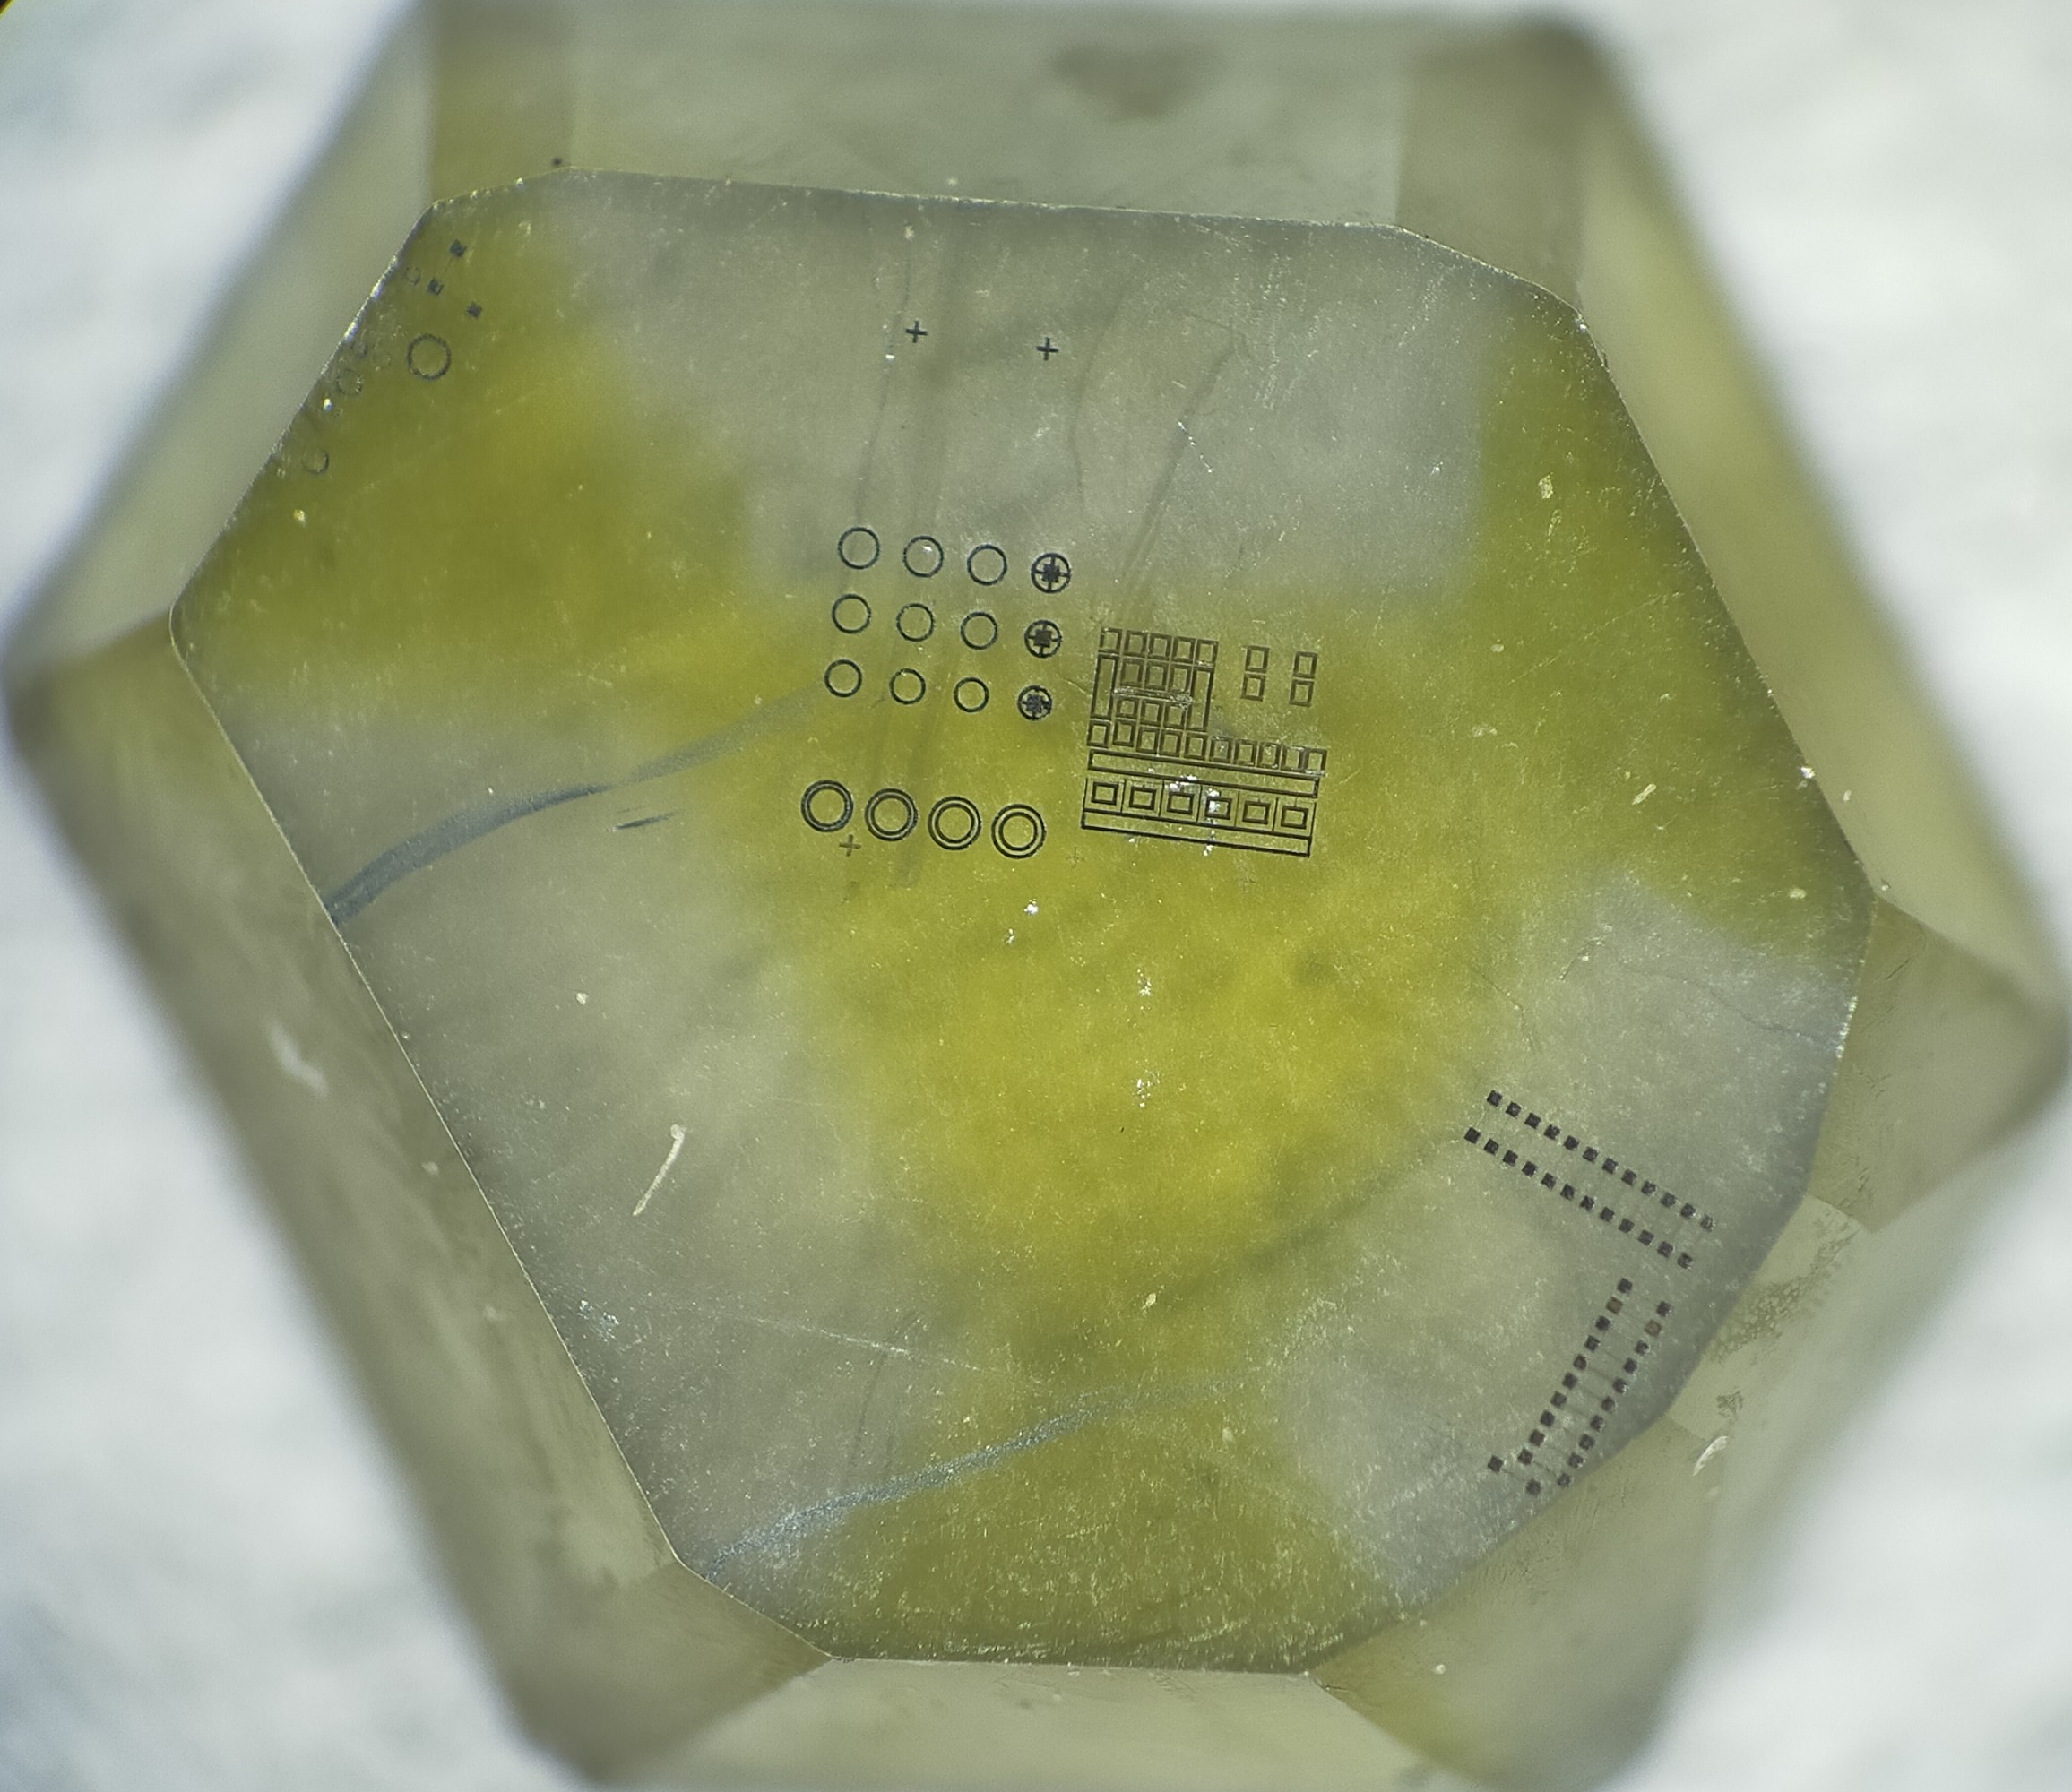
\includegraphics[width=\textwidth]{Chapter7/Figs/Raster/optical front light.jpg}
    \caption{Typical frontal white LED illumination.}
    \label{fig:G_front}
\end{subfigure}
\hfill
\begin{subfigure}[t]{0.47\textwidth}
    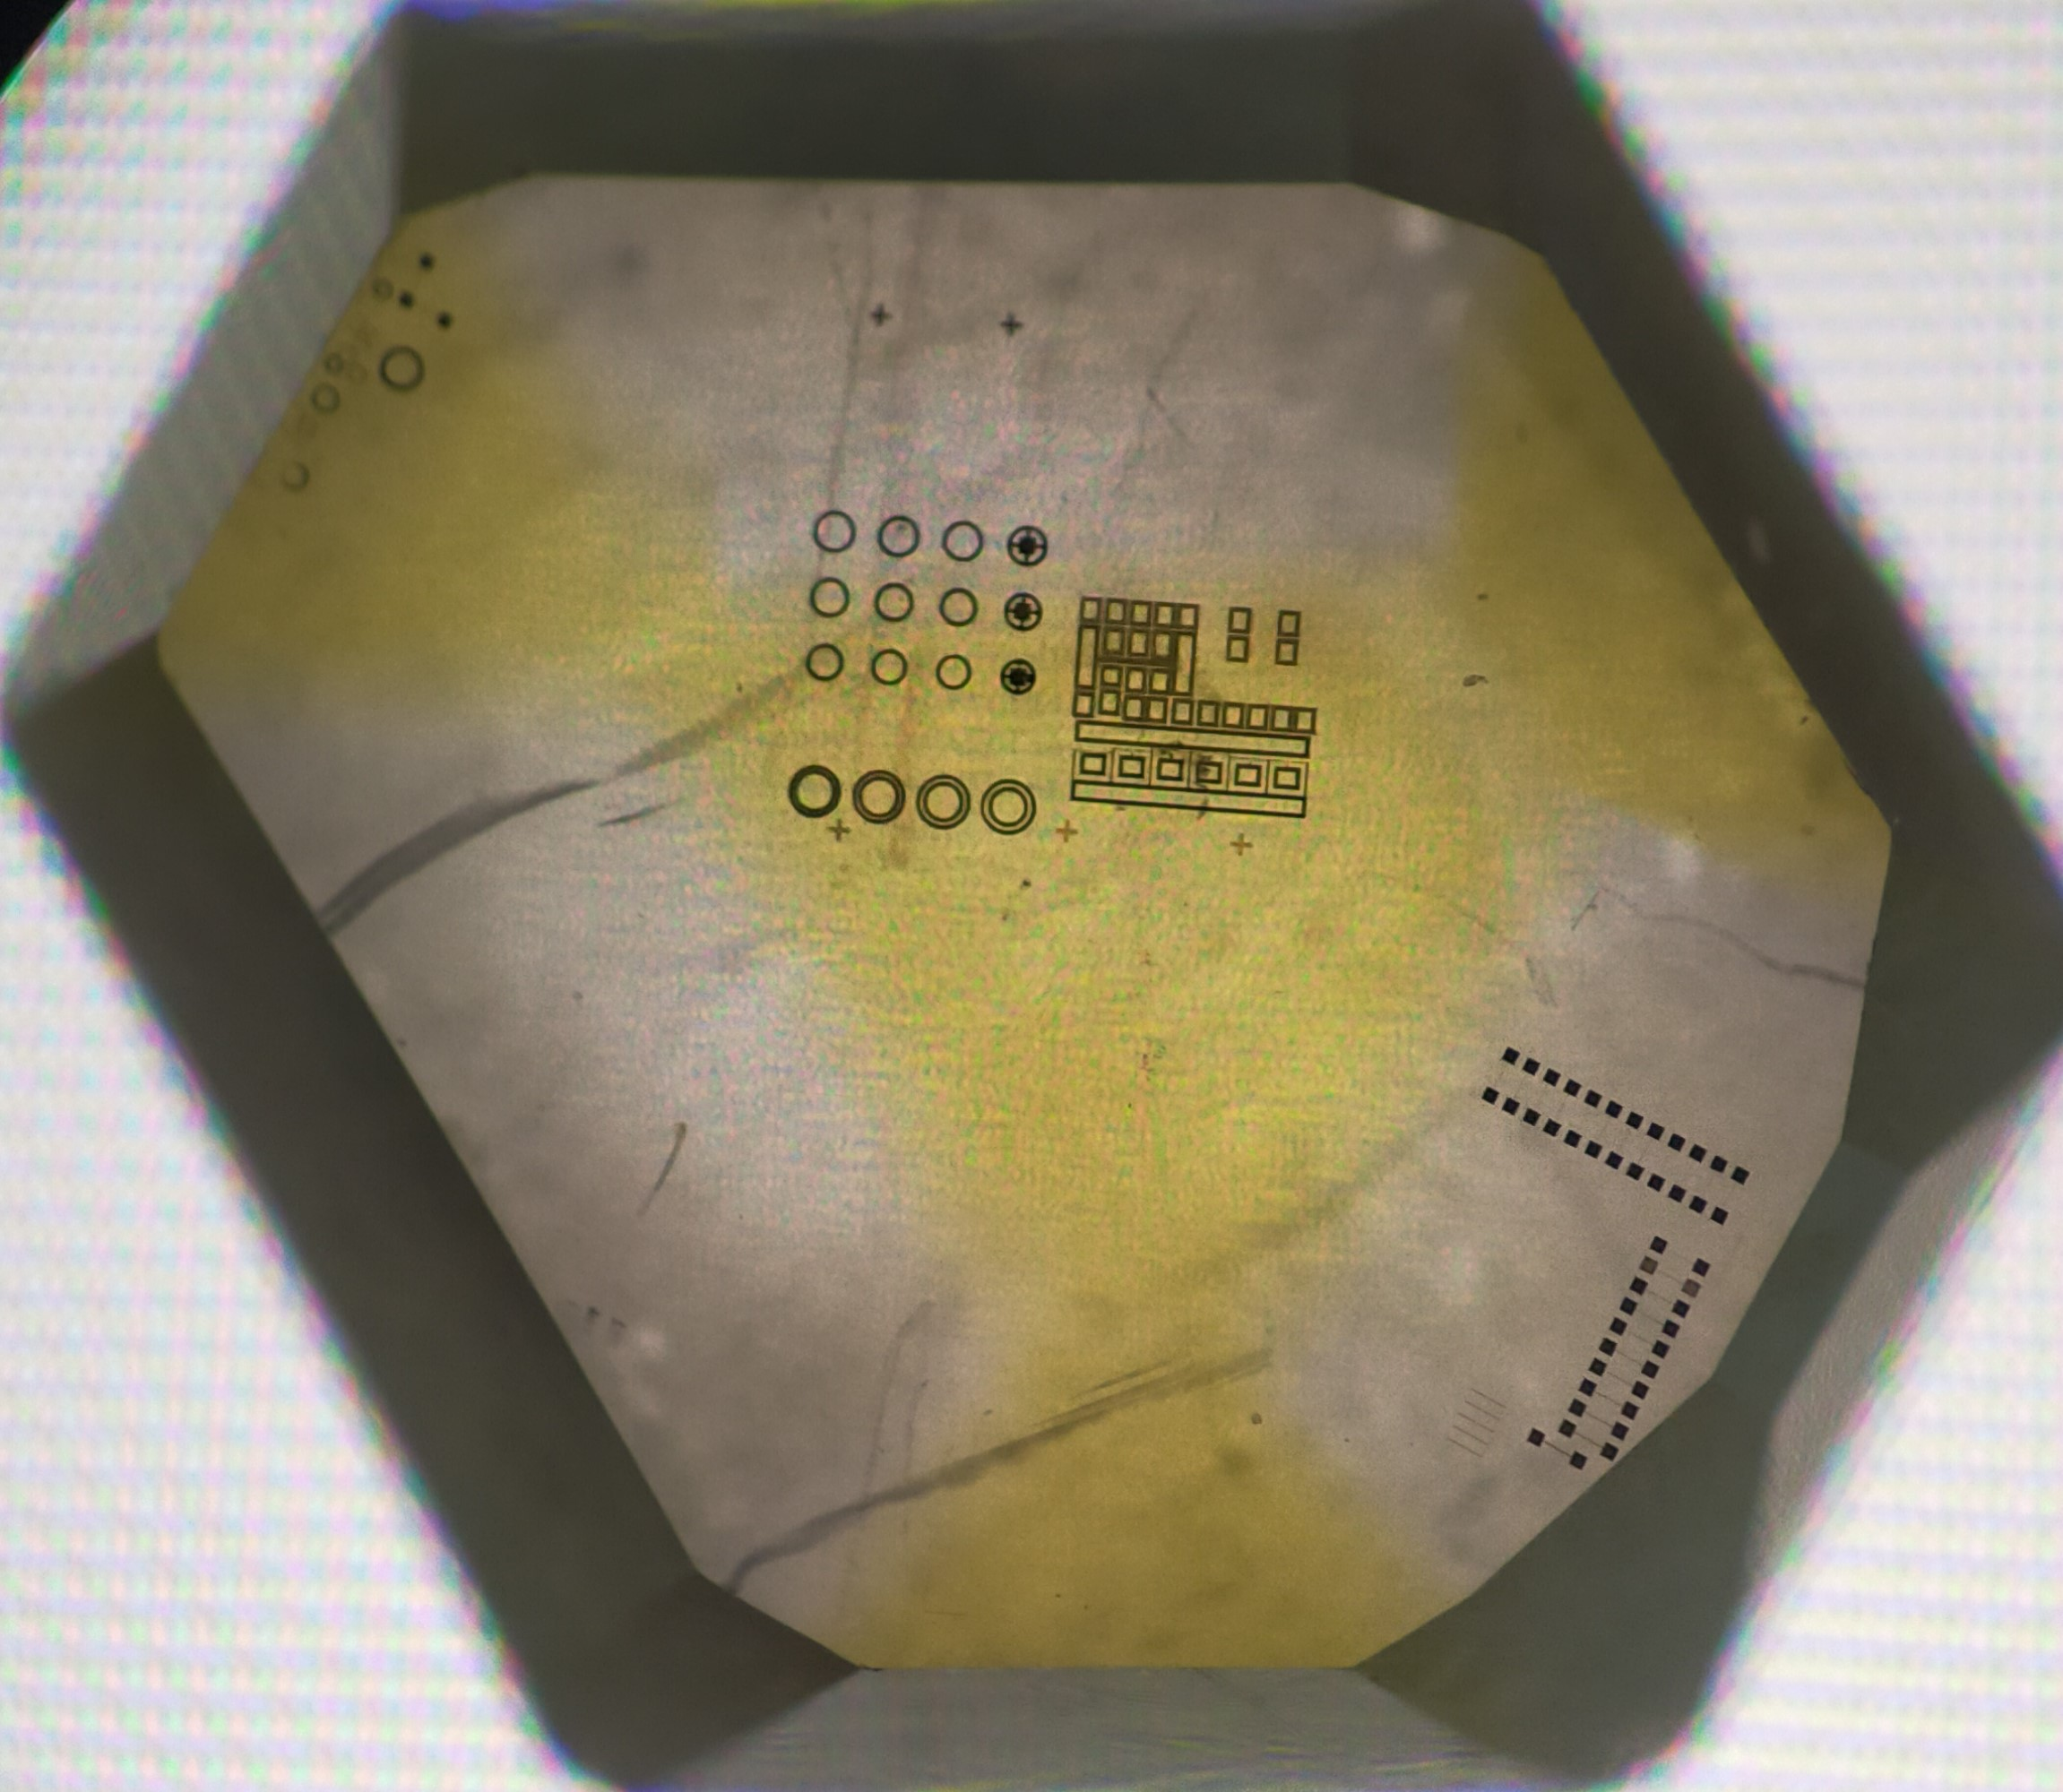
\includegraphics[width=\textwidth]{Chapter7/Figs/Raster/optical back light.jpg}
    \caption{Back-lighting provided by a RGB array.}
    \label{fig:G_back}
\end{subfigure}

\vspace{1em} % this will add some vertical space between the rows

\begin{subfigure}[t]{0.47\textwidth}
    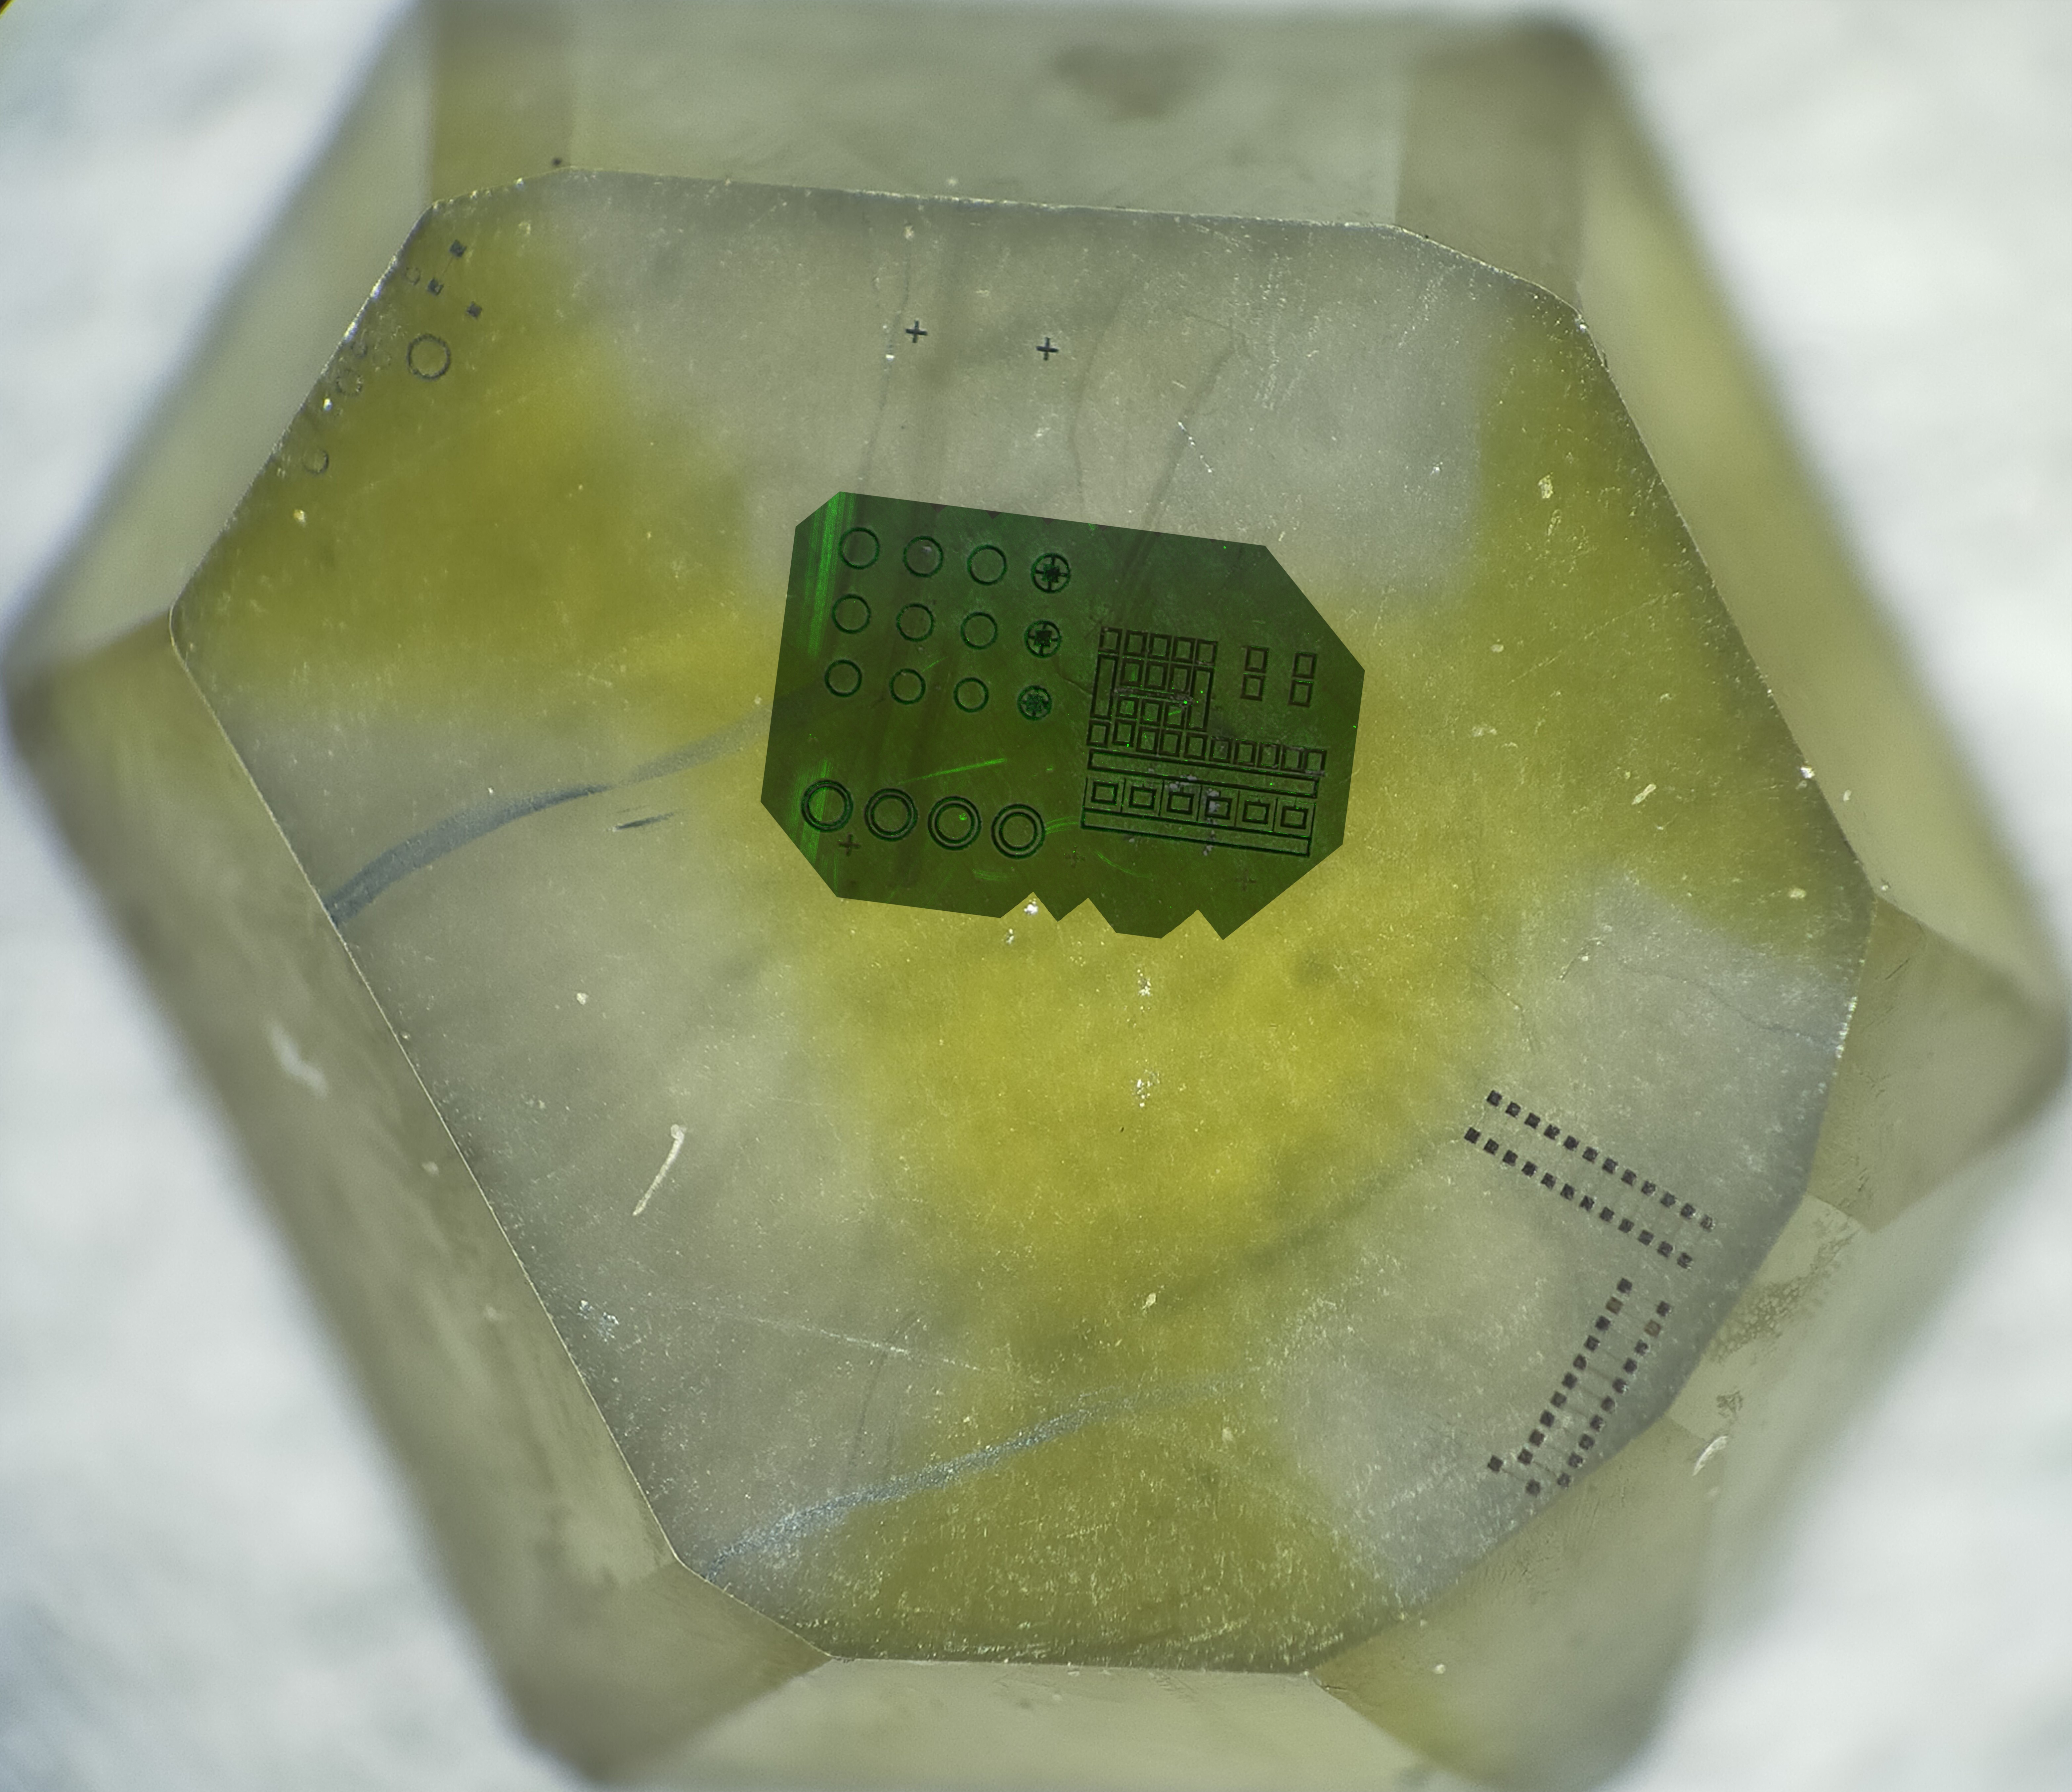
\includegraphics[width=\textwidth]{Chapter7/Figs/Raster/optical front light overlay.jpg}
    \caption{Frontal illumination and fluorescence overlay.}
    \label{fig:G_front_overlay}
\end{subfigure}
\hfill
\begin{subfigure}[t]{0.47\textwidth}
    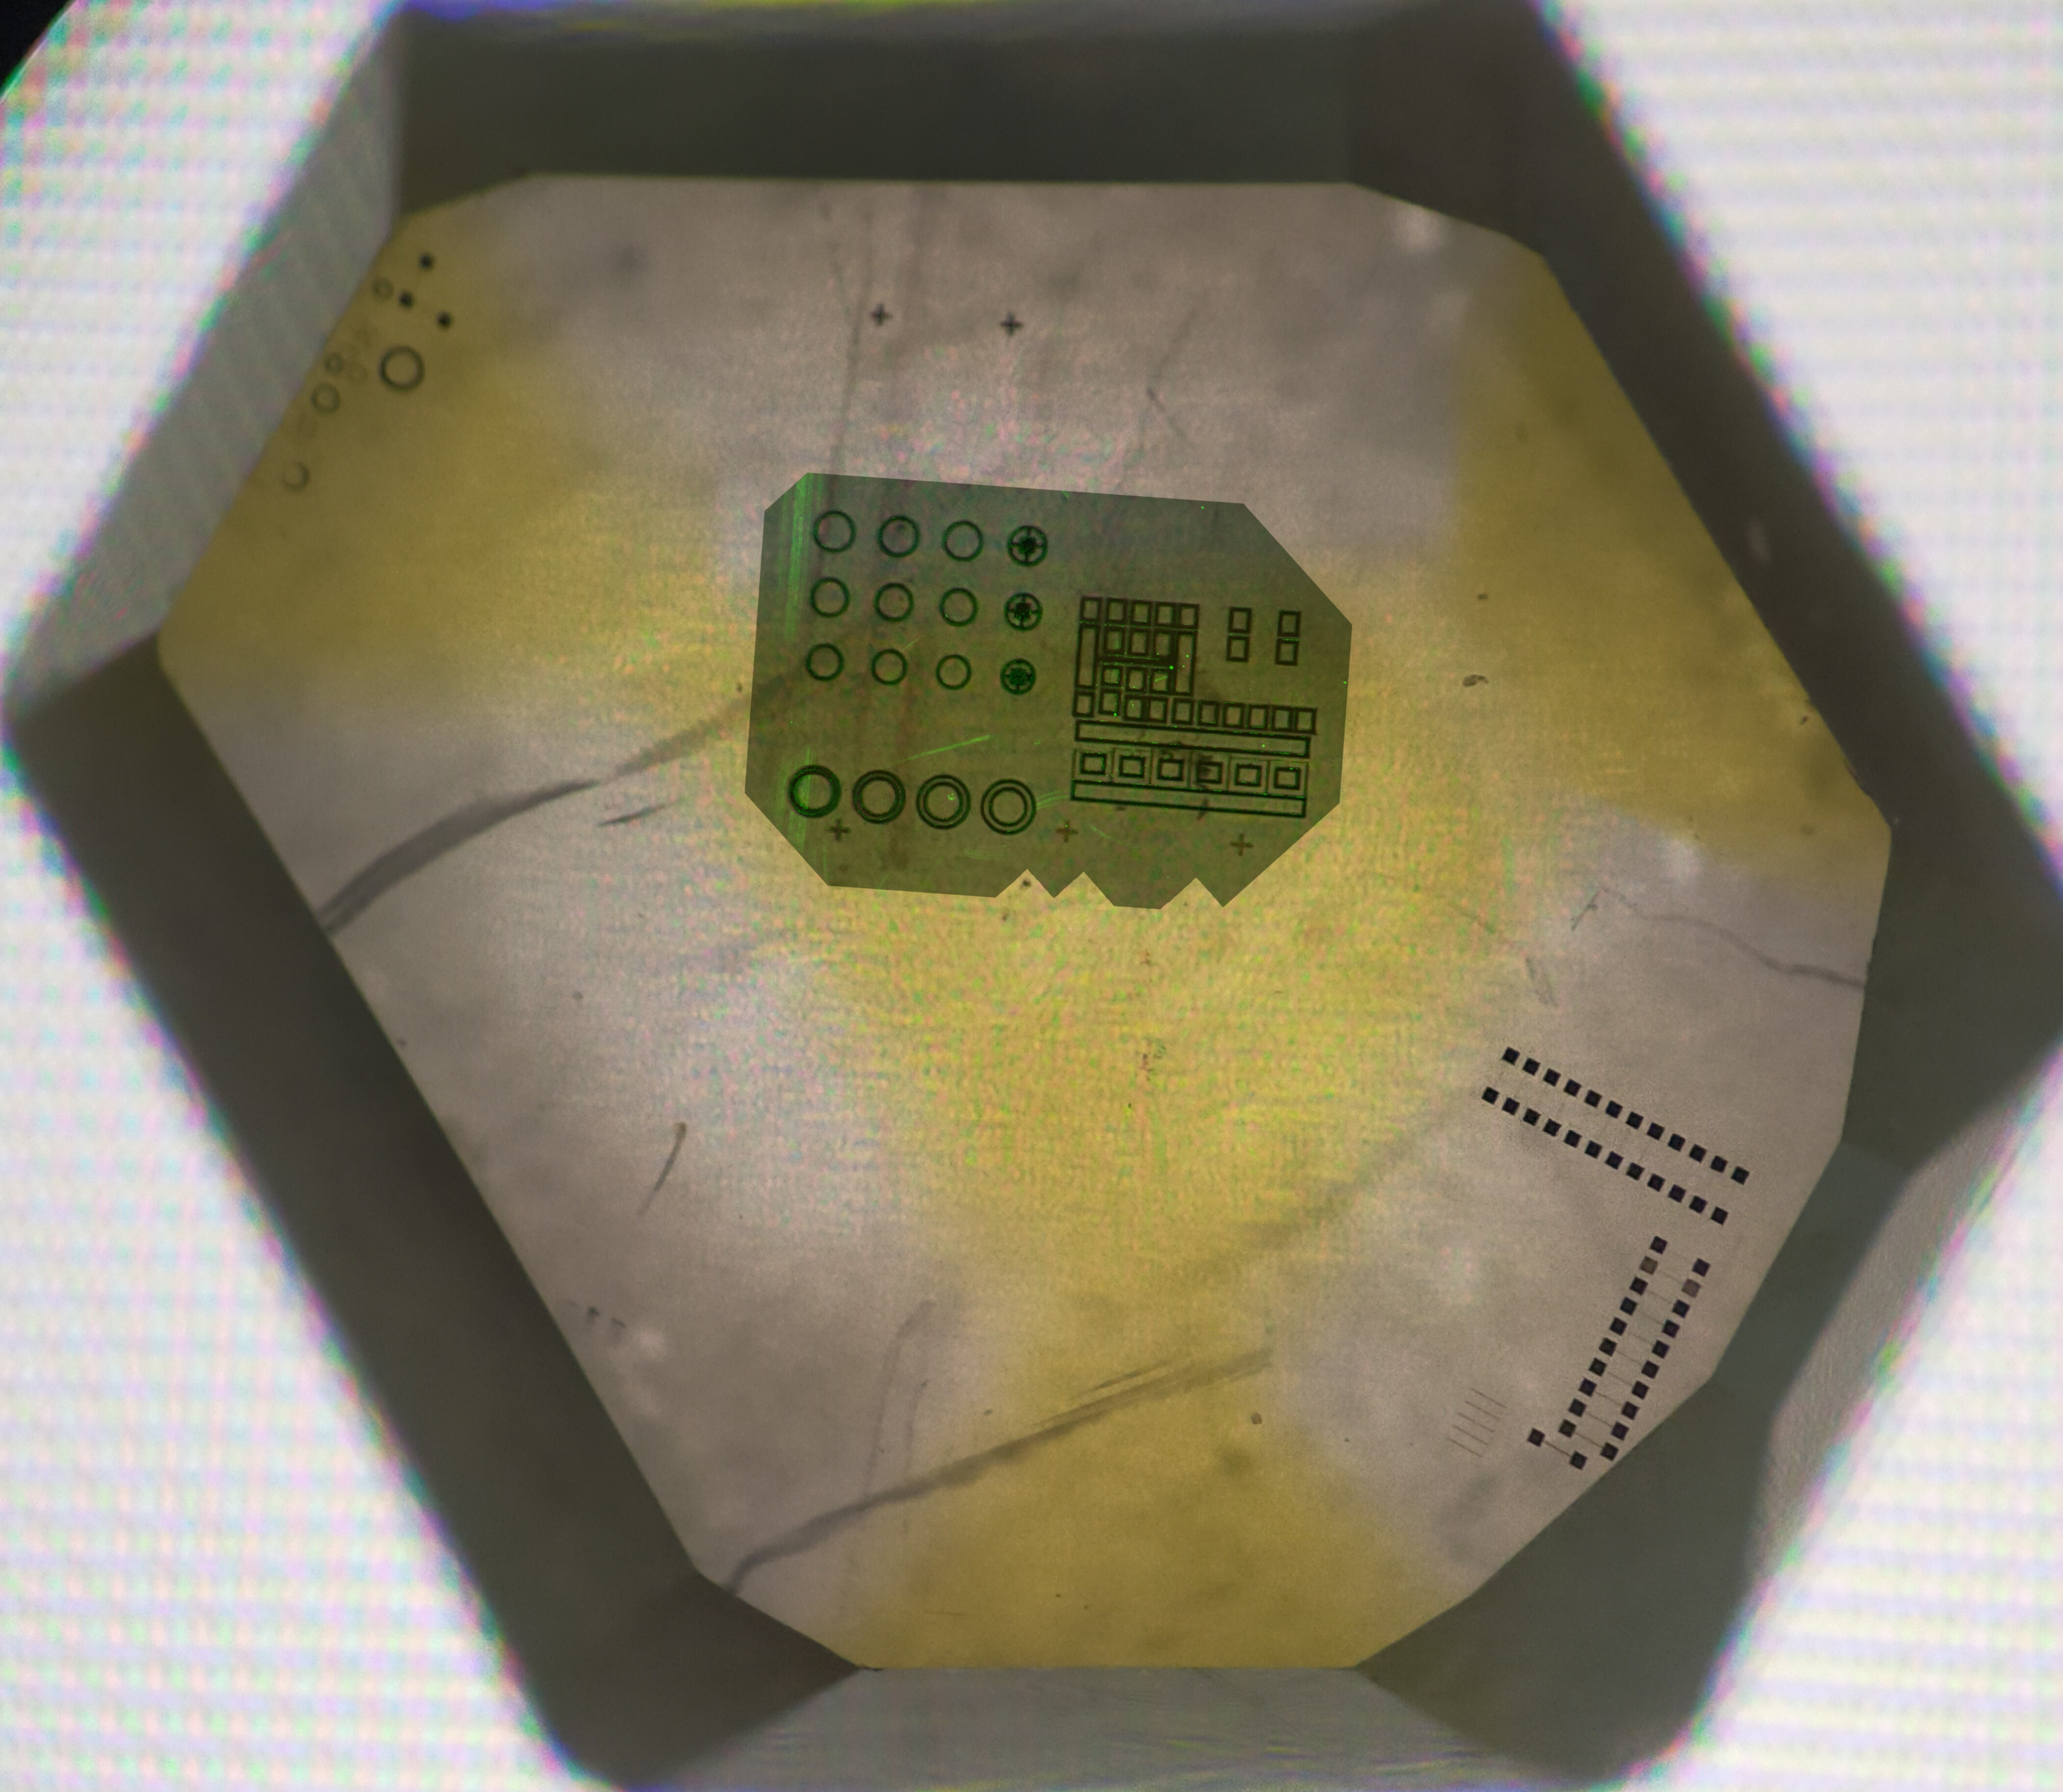
\includegraphics[width=\textwidth]{Chapter7/Figs/Raster/optical back light overlay.jpg}
    \caption{Back-lighting and fluorescence overlay.}
    \label{fig:G_back_overlay}
\end{subfigure}
\caption{Sample G as seen with a 3.6X magnification optical microscope, either direct front facing light or back-lighting, and the fluorescence imaging overlaid on these two images of differing lighting.}
\label{fig:G_illuminations}
\end{figure}

Figure \ref{fig:G_illuminations} includes two different approaches to taking optical images of the sample at a macroscopic scale, to demonstrate the visually apparent growth sectors within the HPHT sample. Back-lighting has a significant impact on the clarity and colour of the different growth sectors, as seen in figures \ref{fig:G_back}, \ref{fig:G_back_overlay}. In particular, a change in the substrate background colour can be observed near the top of the laser processed region, and it is possible to pick out the differing growth regions from the HPHT seed crystal.

\begin{figure}[H]
    \centering
    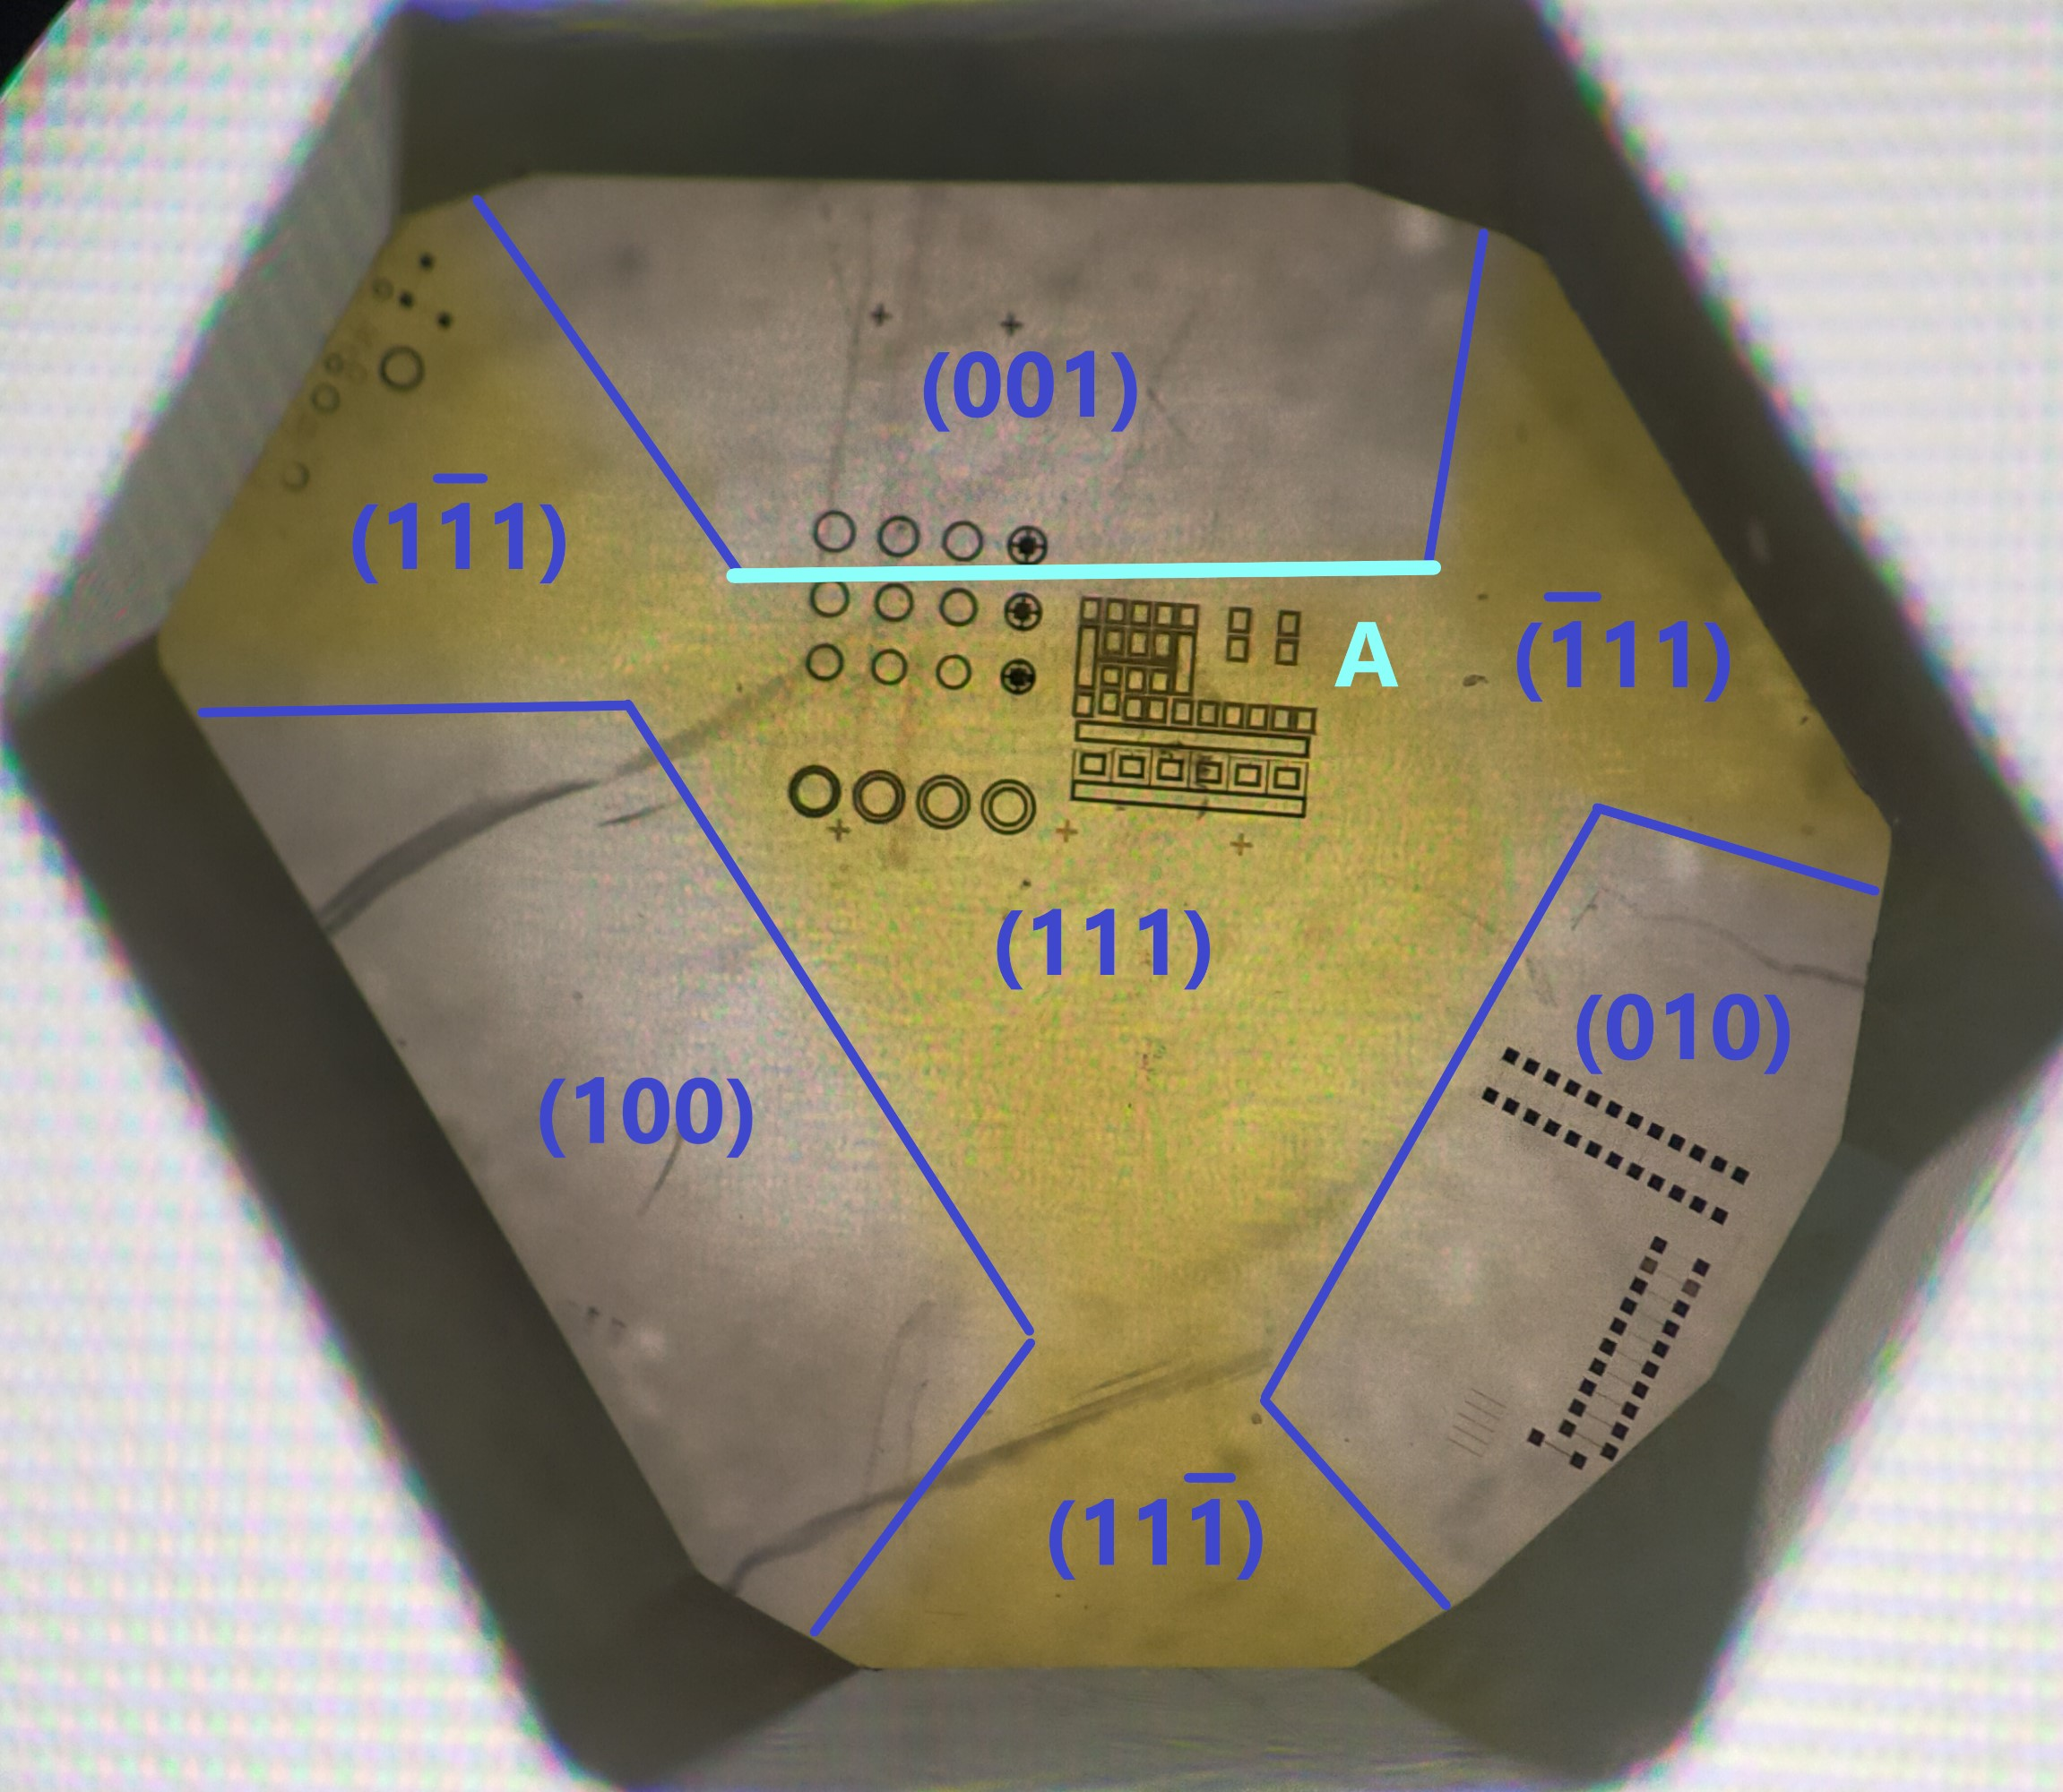
\includegraphics[width=0.8\linewidth]{Chapter7/Figs/Raster/48MP white 5 aperture graphite focus_crop_annotated 1_low.jpg}
    \caption{An annotated version of the back-lit optical microscope image to highlight growth sectors and the significant change in colouration running through the laser processed region.}
    \label{fig:G_annotated}
\end{figure}

Figure \ref{fig:G_annotated} provides an annotated form of figure \ref{fig:G_back}, to clarify the relevant growth sectors and also highlight the distinct change in colour centres that is observed across line A. Comparisons to the fluorescence reveal that the background fluorescence does not change significantly in density despite this change in absorbed/transmitted light.

\begin{figure}[H]
    \centering
    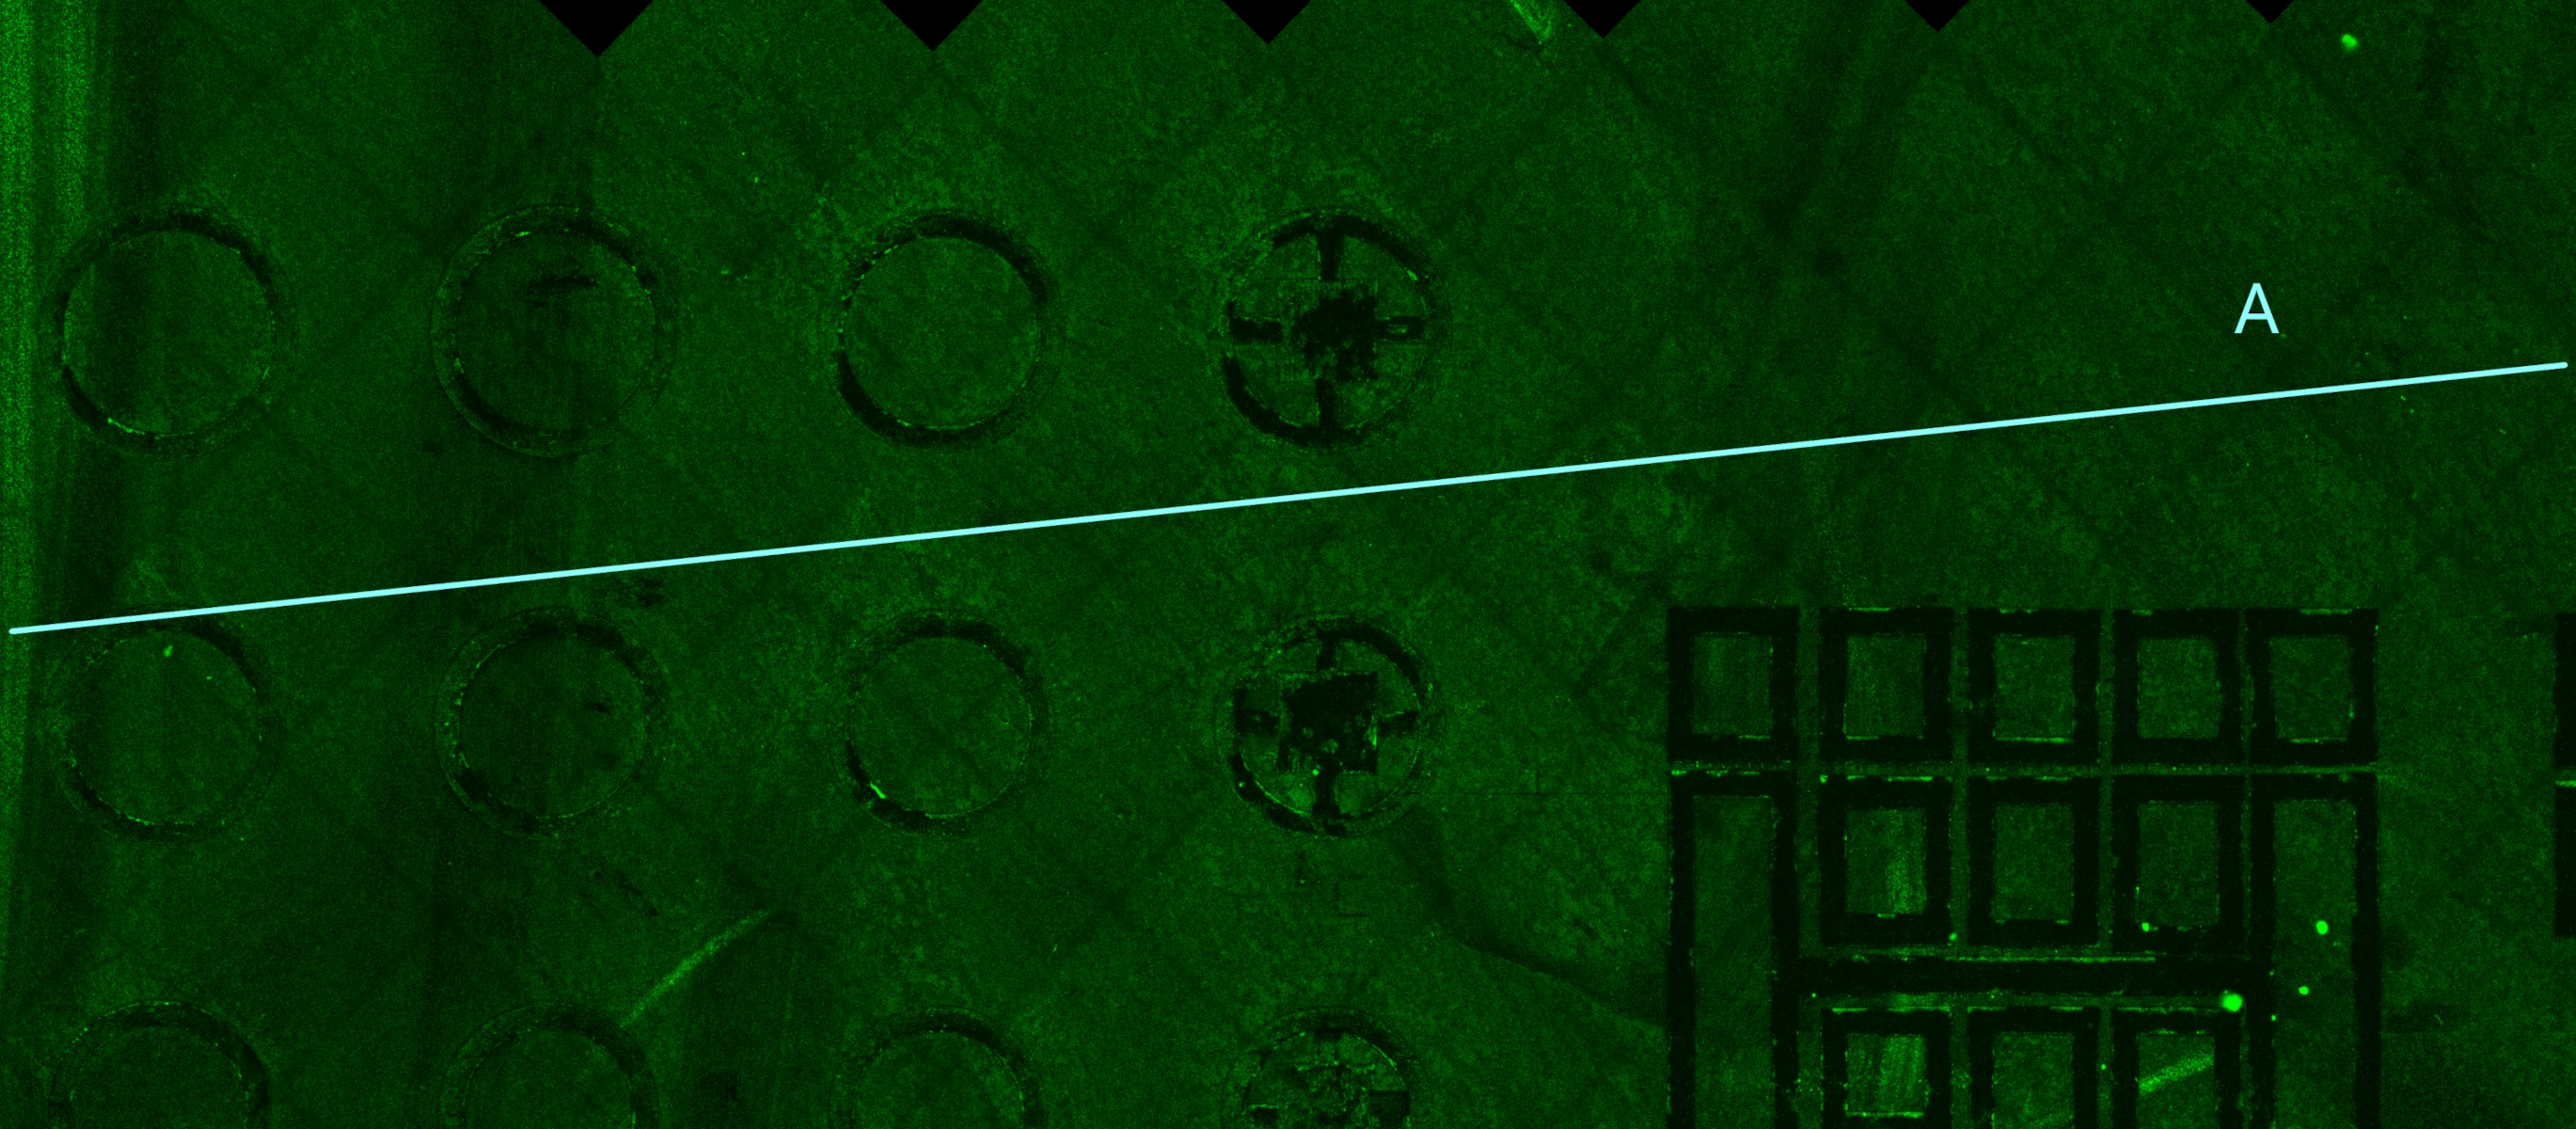
\includegraphics[width=0.8\linewidth]{Chapter7/Figs/Raster/FL_crop 3_low_annotated.jpg}
    \caption{A section of the fluorescence microscopy.}
    \label{fig:fl_crop3}
\end{figure}

In figure \ref{fig:fl_crop3}, the section around line A from figure \ref{fig:G_annotated} is presented to highlight the lack of background growth sector specificity in the observed, relatively constant background fluorescence. The estimated location of the optically observed growth sector change and subsequent change in nitrogen content is indicated by line A.

\begin{figure}[H]
    \centering
    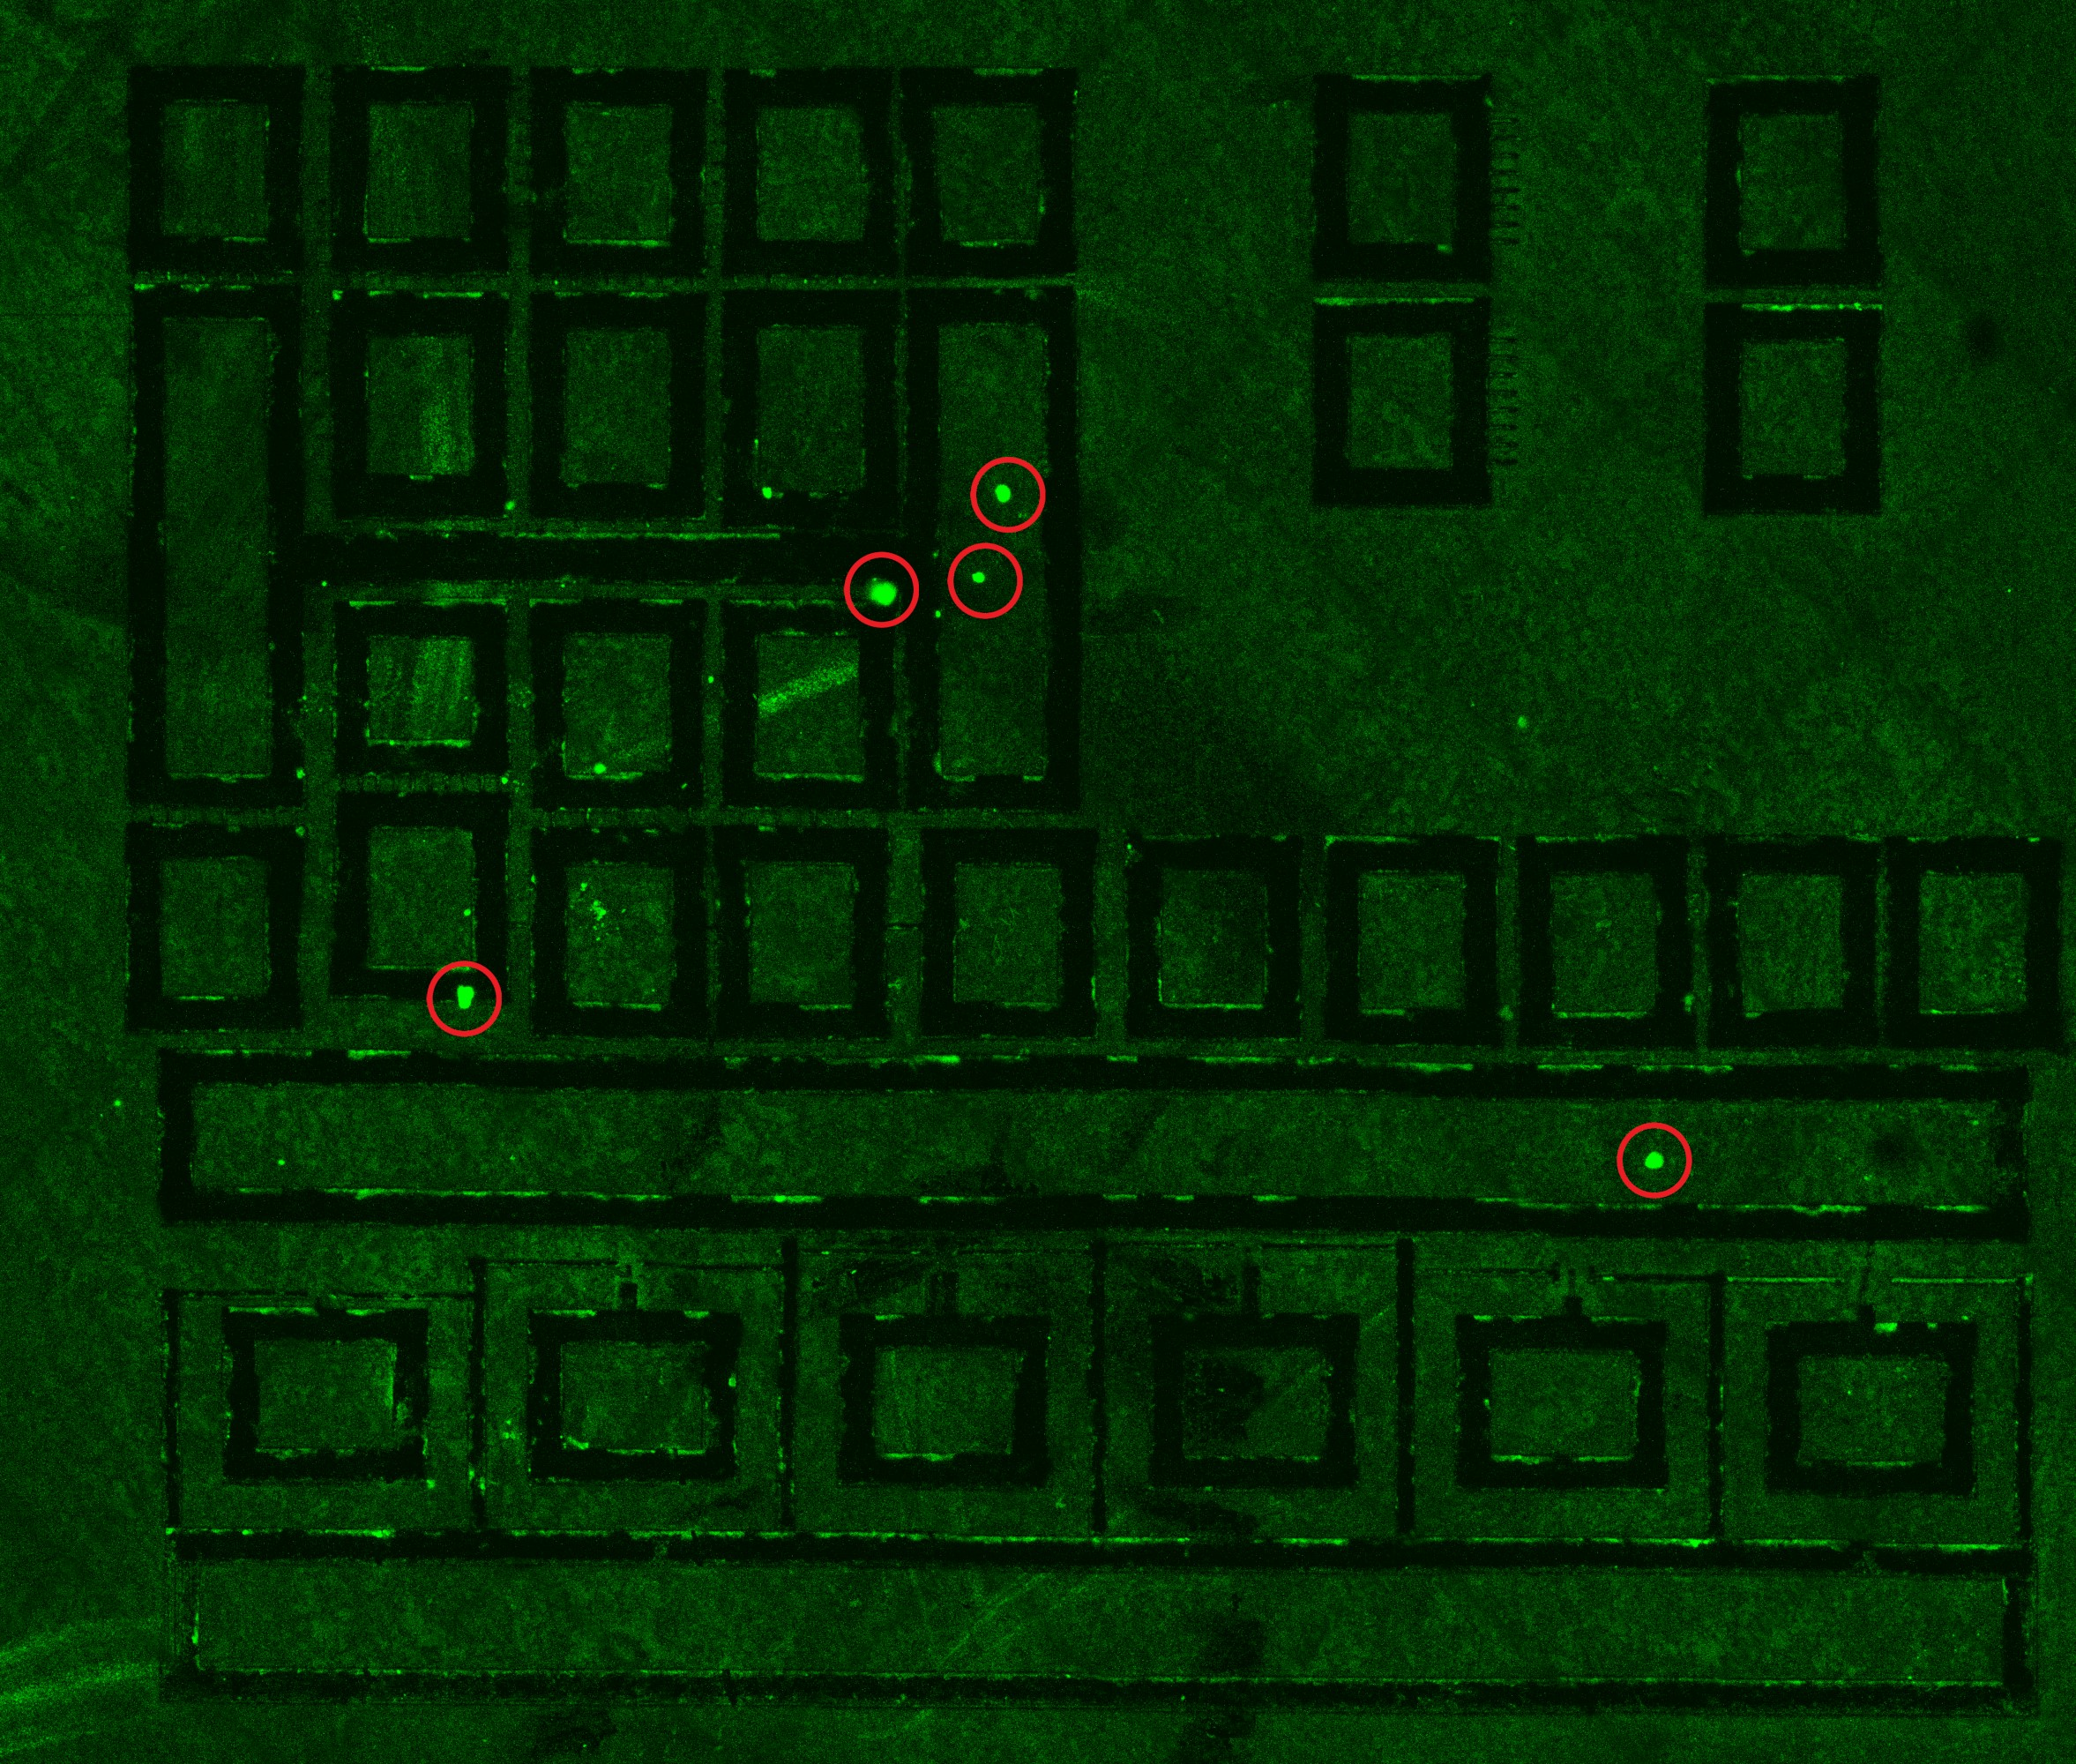
\includegraphics[width=\linewidth]{Chapter7/Figs/Raster/FL_crop 2_low.jpg}
    \caption{A cropped down form of the fluorescent track only, demonstrating the non-uniformity of fluorescence concentrations.}
    \label{fig:fl_crop2}
\end{figure}

Figure \ref{fig:fl_crop2} takes a closer look at the laser processed region of the sample, with only the fluorescence track from the confocal microscopy represented in this image. Note that while the effective spectroscopic analysis of colour filtering did reveal a fluorescence peak in the region of 500--520~\si{\nano\metre}, the green colouration of the fluorescence is a false colour applied to all detected fluorescence used to aid in contrast and the actual colouring may differ. Some fluorescence appears to be present on the surface of the diamond sample, marked by the red circles. In select locations it appears to be on the edge of the laser processed material and yet it is also on the unaltered diamond surface. Due to this inconsistency, it is assumed that this fluorescence is neither due to the substrate or the laser processing, and is likely caused by organic surface contamination despite solvent cleaning steps.

\subsection{Raman Characterisation}
\label{subsec:raman_characterisation}
\begin{table}[ht]
\centering
\begin{tabular}{ccc}
\hline
Position (cm$^{-1}$) & Typical FWHM (cm$^{-1}$) & Assignment \\ \hline
1332                 & 5--10                    & first-order diamond Raman line \\
1355                 & 250                      & $sp^2$ (D peak) \\
1575                 & 100                      & $sp^2$ (G peak) \\ \hline
\end{tabular}
\caption{Raman peaks of interest in diamond and carbon related materials \cite{prawer2004}, \cite{Tuinstra1970}.}
\label{tab:raman_peaks}
\end{table}

As outlined more fully in section \ref{subsec:raman_microscopy}, raman microscopy provides an effective tool for examining the composition of diamond samples. Table \ref{tab:raman_peaks} summarises the relevant peaks of interest for diamond, with the general deconvolution of CVD diamond raman spectra into a diamond line and the D or G modes of amorphous carbon. The relative intensity of diamond to D or G signals is strongly dependent upon excitation wavelength, with the exact mechanisms behind this likely linked to resonance enhancement of the sp$^{3}$ component and decreasing resonance in the sp$^{2}$ component \cite{prawer2004}. Another noteworthy point on excitation wavelength is that the typical rising background seen with excitation sources such as the green argon ion laser at 514.5~\si{\nano\metre} is commonly attributed to strong photoluminescence from nitrogen-vacancy defects \cite{Filik2005}. The laser wavelengths used can be varied depending upon the application, but background subtraction allows for visible peaks even in the case of high background photoluminescence. A laser wavelength of 532~\si{\nano\metre} was used with the LabRam HR-800 Jobin Yvon at the SAgE analytical facility for the purposes of characterising the laser processed device structures and heavily phosphorous doped surface layer. 

One other relevant consideration for raman spectroscopy of samples which have two components, such as amorphous carbon, is the relative polarisability of the components. $\pi$ bonds formed by sp$^{2}$ hybridised carbons have a higher polarisability than that of the $\sigma$ bonds within sp$^{3}$ hybridised carbon, which results in a larger raman cross-section \cite{Zhang2022}. Additionally, $\pi$ bonds are resonantly enhanced with visible excitation lasers while $\sigma$ bonds are not. This tends to lead to a dominance of sp$^{2}$ signal in samples where even low ($\sim20$\%) fractions of sp$^{2}$ material is present \cite{Ferrari2004}. 
To summarise, for single crystal diamond the position and FWHM of the diamond line, and relative intensity of the diamond line to the G and D peaks are used as crude measures of crystallinity \cite{Bennett2024}. This is due to single crystal diamond only displaying the first order diamond line while grain boundaries in polycrystalline films will produce varying intensities of D and G peaks depending upon the grain sizes \cite{Bachmann1994}. At the extreme of pure graphite, only the crystalline G peak remains, while in all other forms of graphitic materials the disorder D peak appears \cite{Tuinstra1970}. 

\subsubsection{Amorphous Carbon}
Amorphous carbon (a-C) is made up of unstructured mixtures of sp$^{3}$ and sp$^{2}$ hybridised carbon. The properties of such material is dependent upon the ratio sp$^{3}$ and sp$^{2}$ bonding, with amorphous carbon films of high sp$^{3}$ content forming a harder material which is more transparent and of higher resistivity than of materials with high sp$^{2}$ content \cite{Suzuki20042}. Films of high sp$^{3}$ content are also highly stressed, and are hence more likely to delaminate from the substrate surface. Amorphous carbon films can also be hydrogenated, and this is quite common for CVD grown films \cite{Robertson1996}. These hydrogenated amorphous carbon films are softer, more stable, and will tend to be more transparent than hydrogen-free films. There is also a variable range hopping conduction mechanism between clusters of hydrogenated sp$^{2}$ carbon in amorphous carbon films which may represent a possible conductive path in the case of laser processed diamond \cite{Tomidokoro2021}.

\begin{figure}[H]
    \centering
    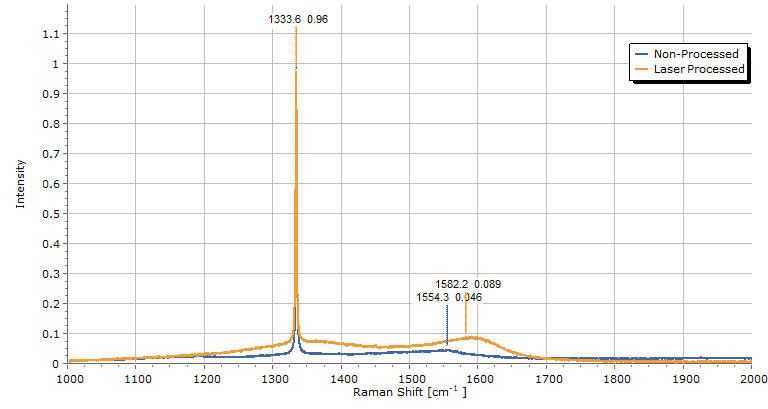
\includegraphics[width=\linewidth]{Chapter7/Figs/Raster/raman_both.png}
    \caption{Relative intensities of raman spectra for untreated and laser-treated portions of sample G. The spectra are normalised such that the sp$^{3}$ peak for both examples is set to 1.}
    \label{fig:raman_both}
\end{figure}

\begin{table}[ht]
\centering
\begin{tabular}{cccc}
\hline
Material Type & Raman Shift (\si{\per\centi\metre}) & Relative Intensity & FWHM (\si{\per\centi\metre}) \\ \hline
Non-Processed & 1334 & 1.00 & 2.24 \\ 
Non-Processed & 1554.3 & 0.08 & 63.81\\
Laser Processed & 1333.6 & 0.99 & 2.28 \\
Laser Processed & 1582.2 & 0.12 & 29.53 \\ \hline
\end{tabular}
\caption{Raman spectrum data comparing non-processed and laser-processed materials.}
\label{tab:raman_data_combined}
\end{table}

In figure \ref{fig:raman_both}, two different raman spectra are plotted, which represent a portion of the sample that has been laser processed, and another region which was well away from any laser processing on the phosphorous doped diamond surface. The exact location used for the laser processed region is indicated by the red square in figure \ref{fig:raman_section}, which was chosen due to the large radius of laser processed material that surrounds the centre point. While it is not possible to guarantee that the laser spot will only be absorbed and otherwise interact with the visibly darkened, laser affected region of diamond, this was chosen to maximise any sp$^{2}$ raman signal. 

\begin{wrapfigure}{r}{0.4\linewidth}
  \centering
  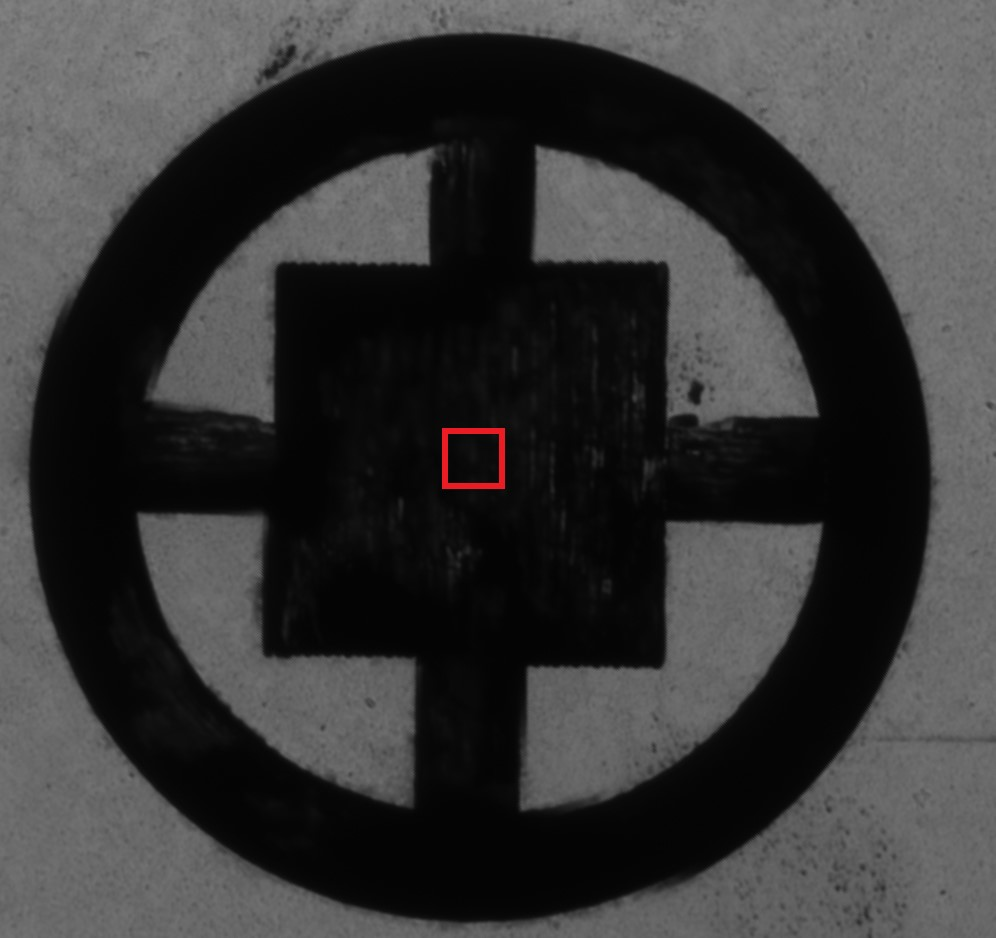
\includegraphics[width=\linewidth]{Chapter7/Figs/Raster/raman_section_anno.jpg}
  \caption{A 488~\si{\nano\metre} confocal microscope image of the raman area, showing the section of the sample under investigation.}
  \label{fig:raman_section}
\end{wrapfigure}

The "Non-Processed" region was strategically chosen on the opposite side of the diamond sample, away from any laser-written areas. However due to the optical transparency of diamond, it remains a slim possibility that any sp$^{2}$ raman signal from this location may be due to a distant, laser processed portion. 

As shown in figure \ref{fig:raman_both} and table \ref{tab:raman_data_combined}, there is a shift in what may be considered the G peak, rising from a small hump that may be attributable to the highly phosphorous grown surface layer, to a moderate peak in the raman spectra of laser processed material. Both spectra show a small shift in the 1332~\si{\per\centi\metre} diamond peak, and they also have a similar FWHM for this line. While there is a visible difference between these two raman spectra, it is difficult to say that the laser processed material represents highly graphitised material, especially compared to the drastic relative shifts that are typical for laser modified diamond \cite{kononenko1998}, \cite{kononenko:2008}. However, the rise in G peak does indicate a change in the material structure due to the laser processing, in accordance with a rise in sp$^{2}$ carbon content.

\section{Laser Graphitisation for Ohmic Contacts}
\label{sec:laser_graphitisation_for_ohmic_contacts}
As demonstrated in sections \ref{subsec:fluorescence_characterisation} and \ref{subsec:raman_characterisation} via various microscopy techniques, the laser processing of a highly phosphorous doped surface layer on a \hkl(111) oriented sample has resulted in a clear change in the diamond crystal structure following the intended design of electronic devices. AFM characterisation has shown that the topographical features vary in the ablation associated with this processing. The fluorescent behaviour of these features is noteworthy, indicating that while this material absorbs visible light as expected for diamond with broken sp$^{3}$ bonds, its optical properties differ from those of other laser-processed regions. While the models for this fluorescence remain speculative, the primary concern is that of the electrical characteristics, and whether or not the features of ablation and fluorescence impact the function of electrical devices created using this processing step. To that end, the electrical characterisation presented here follows a bottom-up approach, starting with tests on surface-written wires to confirm ohmic behaviour, indicative of the breakdown of diamond's sp$^{3}$ bonds. Subsequent tests on a TLM type structure and an emitter structure further explore this behaviour, and attempt to utilise this property.

\subsection{Testing of Surface Graphitic Wires}
\label{subsec:testing_of_surface_graphitic_wires}
\begin{figure}[H]
    \centering
    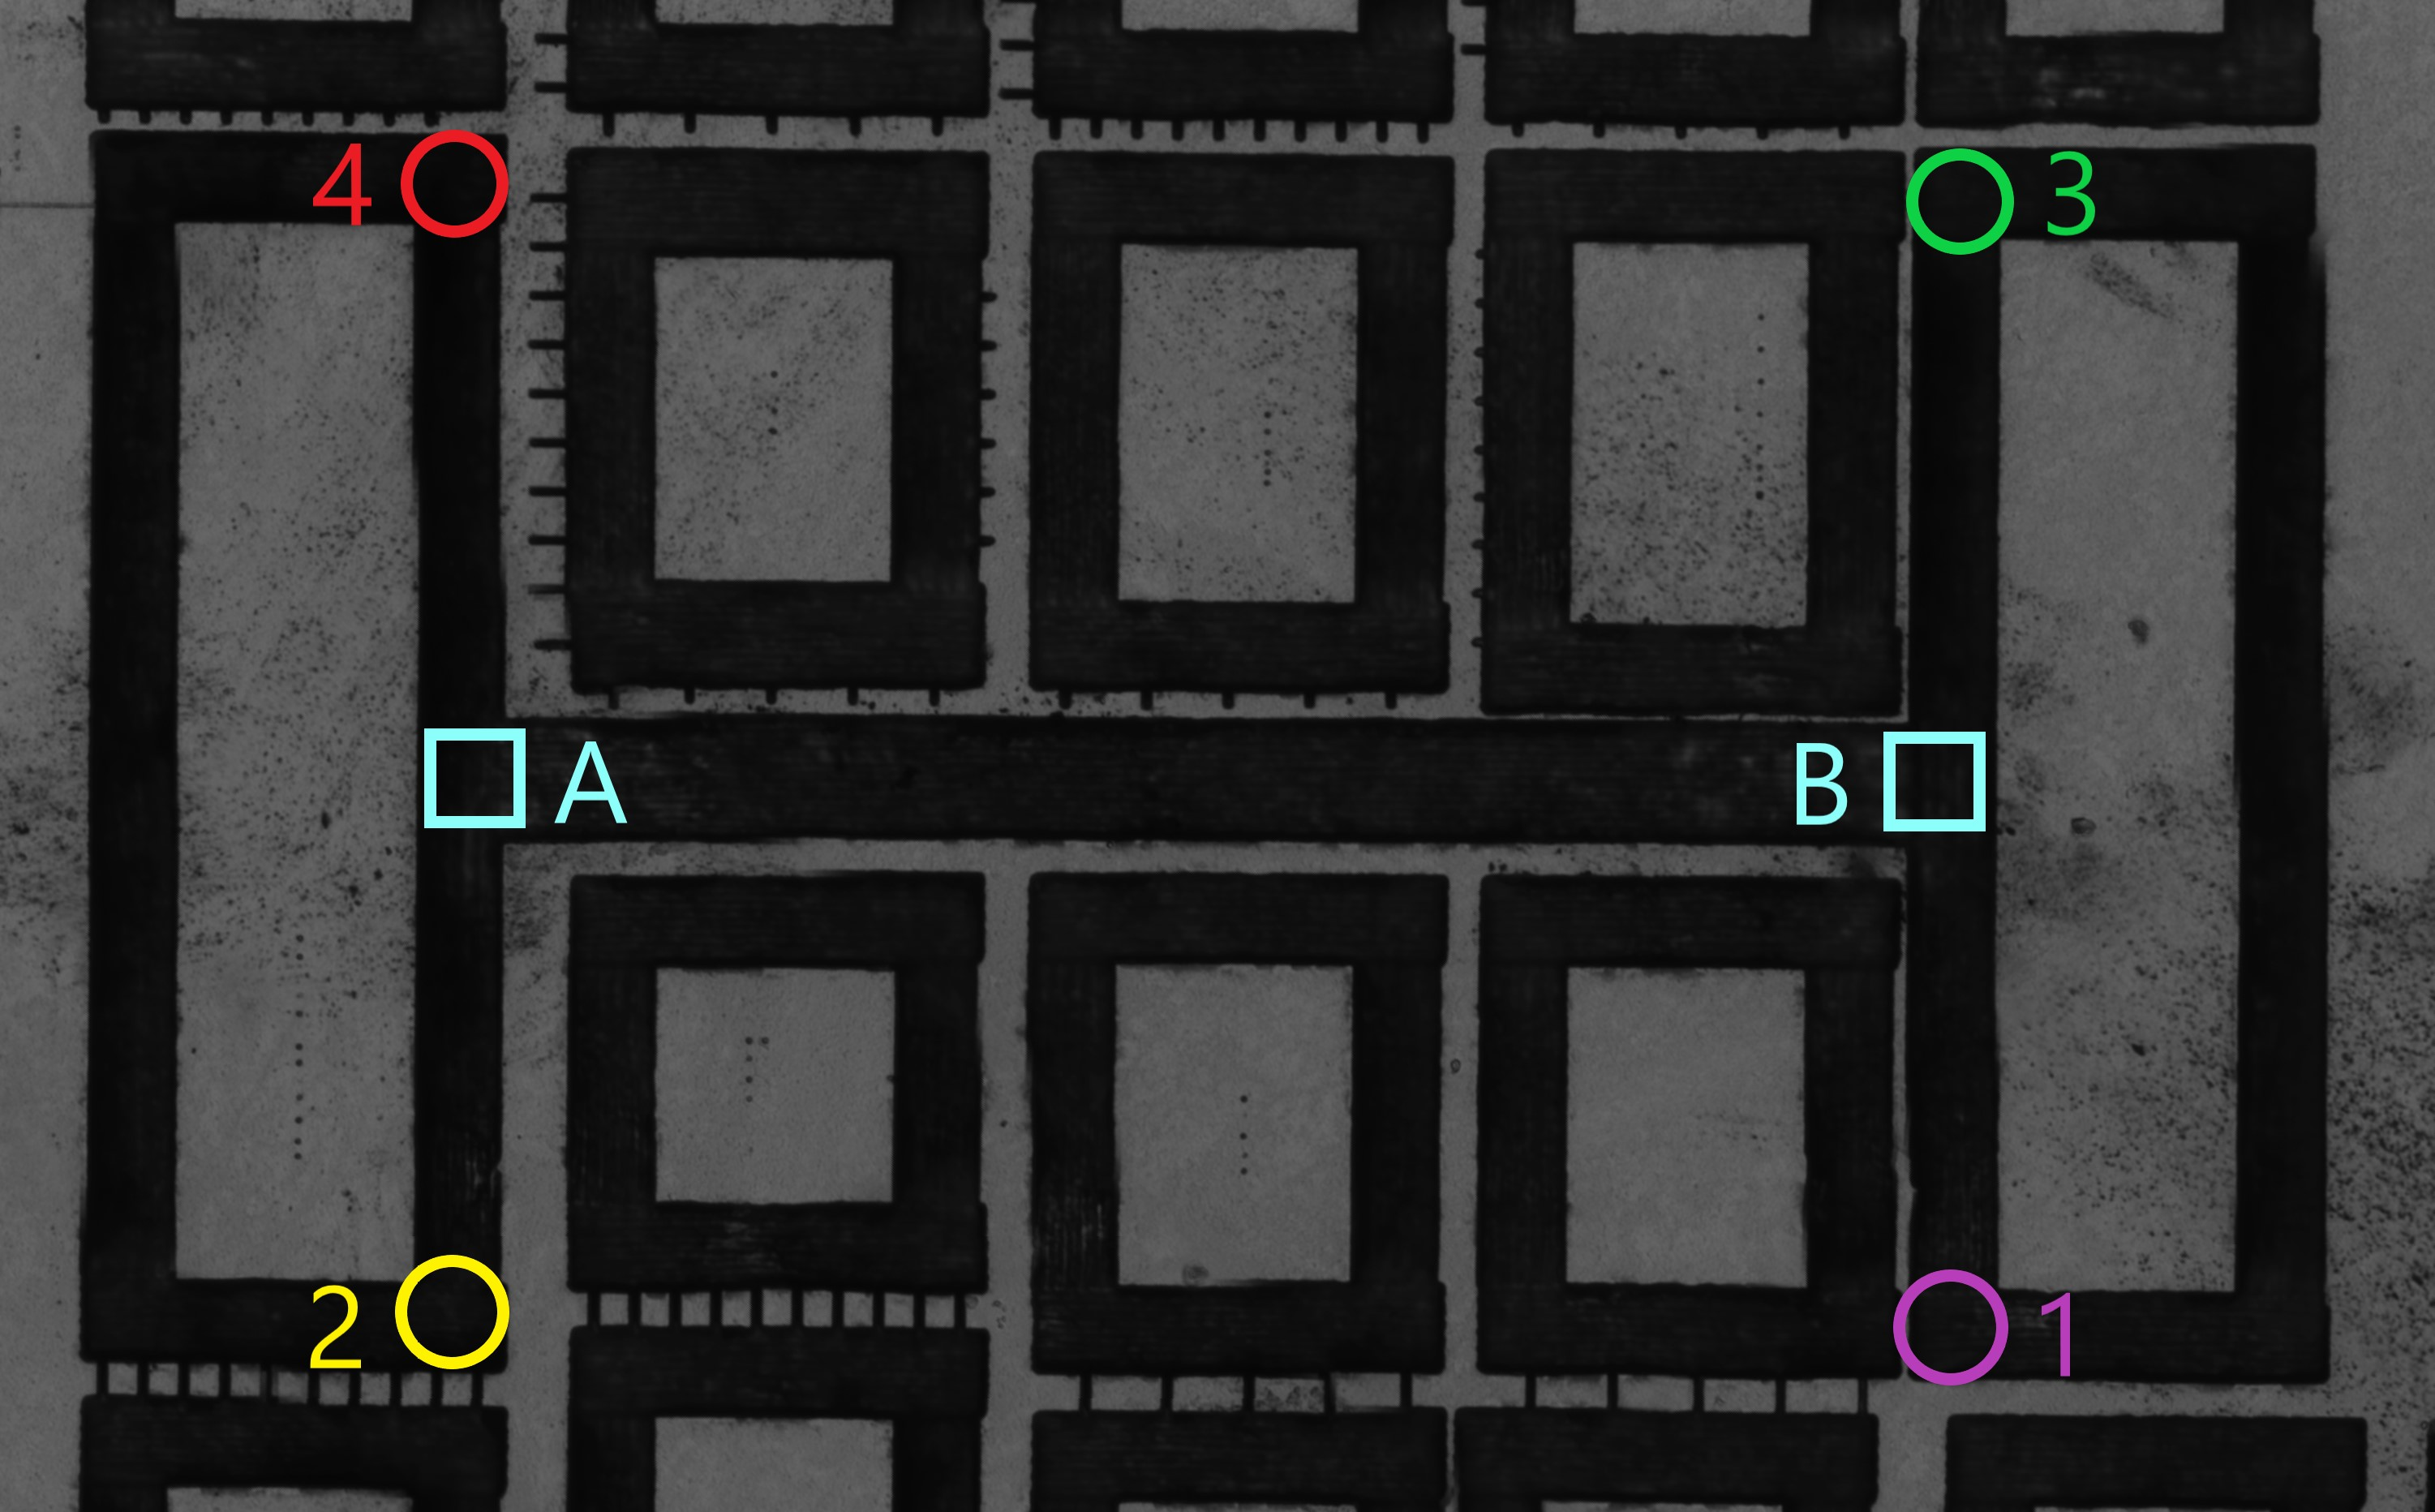
\includegraphics[width=\linewidth]{Chapter7/Figs/Raster/big_bone_esid_annotated.jpg}
    \caption{The I-shaped laser processed conductivity test structure.}
    \label{fig:big_bone_esid}
\end{figure}
Figure \ref{fig:big_bone_esid} shows the simple wire structure that was designed to allow for preliminary electrical characterisation. The annotated shapes indicate the positions of six different electrical probe positions that were used to make contact with the laser processed diamond surface. For reference, these are labelled such that the two aqua squares A and B represent the first set of electrical trials, followed by the circles used for the second set of trials which are labelled 1--4 starting from the bottom right and increasing in the anti-clockwise direction.

As indicated in figure \ref{fig:big_bone_measurements}, the top 10~\si{\micro\metre} wide wires have a length of 70.5~\si{\micro\metre}, and the bottom wire has a length of 65.5~\si{\micro\metre}. This slight difference in path length should result in a reduced resistance in the situation where the induced current is measured across probes 1 and 2, when compared to probes 3 and 4. Note that the 14~\si{\micro\metre} cross-bar wire has a length of 174~\si{\micro\metre} when measured from the edges of the 10~\si{\micro\metre} wires. This substantial length allows for a relatively large distance of laser processed wire to be tested, with the additional benefit of a change in width allowing for comparison with the slightly narrower 10~\si{\micro\metre} wires.

\subsubsection{Electrical Probe Placement Error Estimation}
\begin{wrapfigure}{r}{0.4\linewidth}
  \centering
  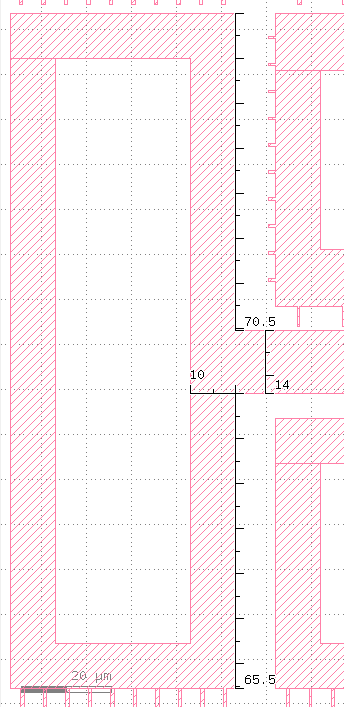
\includegraphics[width=\linewidth]{Chapter7/Figs/Raster/big_bone_measurements_2.png}
  \caption{A snippet of the design for the wire testing region.}
  \label{fig:big_bone_measurements}
\end{wrapfigure}
\label{subsubsec:electrical_probe_placement_error_estimation}
One detail worth including at this stage is a discussion of the electrical probe tips that were used to make contact to the laser processed wires. Standard micro-probes usually have tip radii of the order of 10~\si{\micro\metre}, and naturally trying to make good contact with wires that are 10~\si{\micro\metre} in width is a challenging prospect, especially due to the ablation of material in the centre of the wire. It would be exceedingly difficult to reliably place tips with a diameter greater than that of the surface features in the correct place. Tip placement relies upon the tip curvature and surface topology, which as previously noted is that of surface trenches, of smaller widths than that of the optically observed laser processed wires. It is physically impossible to place such a large tip into the trench, and contact would only be made on the very edges of the probe tip, reducing the surface area of the contact significantly and potentially inducing a large contact resistance if no good contact is formed. For that reason, probe tips with a full tip diameter of 10~\si{\micro\metre} were used to make contact to the surface wire structures directly. The circles used to represent the probe positions in figure \ref{fig:big_bone_esid} hence show a rough approximation of the size of the tips used in the electrical characterisation, with radii at 5~\si{\micro\metre}. 

Despite great care in the positioning of these micro-tips, it is also important to note that the exact positioning of the probes relative to the wires being measured is an important source of error. The exact length of wires under investigation is a crucial variable for the calculation of measured resistivity and conductivity across differing wires. Hence, the variation of micron-scale positioning must be accounted for. The minimum potential error in electrical path length may be given by $2\times$ the tip radii, which is $\pm10$~\si{\micro\metre}. This is the minimum due to the tip radii themselves, but also sets a lower bound for the potential of inexact placements during the experimental process itself, as the probe tips may not necessarily be ideally situated in the locations marked on figure \ref{fig:big_bone_esid}. While the placements were aided by an optical microscope, the precision and reliability with micropositioners establishes a hard limit of $\pm5$~\si{\micro\metre} per probe tip. In particular for these smaller than average probe tip radii, the identification of physical contact was challenging to observe, with any additional force applied to the probe leading to significant bending of the probe tip and subsequent translation of the probe tip along the wire. Larger tip radii allows for a probe tip with greater resistance to deformation, but as previously discussed the tip radii was strategically chosen to allow for the best possible contacts to be made to 10~\si{\micro\metre} wide wires, leading to this potential error in placement but reducing the issue of contact formation itself.

\begin{table}[ht]
\centering
\begin{tabular}{|c|c|c|c|}
\hline
Electrical Path & Path Length (\si{\micro\metre}) \\
\hline
A-B & $164$  \\
1-3 & $140$  \\
2-4 & $140$  \\
1-2 & $295$  \\
3-4 & $305$  \\
1-4 & $301$  \\
3-2 & $301$  \\
\hline
\end{tabular}
\caption{Summary of electrical path lengths and the corresponding error due to probe placement. The error in path length is taken as $\pm10$.}
\label{table:probe_placement_error}
\end{table}

Table \ref{table:probe_placement_error} provides a brief summary of the electrical path lengths between the different probe locations. The standard minimum error is more notable for the shortest electrical paths, such as A-B or 1-3, 2-4, when it is expressed as a percentage error of the path length. However, by taking this into account the conclusions of electrical measurements taken between these probe locations can be considered fairly.

\subsubsection{Laser Writing Thickness}
\label{subsubsec:laser_writing_thickness}
One final detail is necessary to consider the effective resistivity of the laser processed surface wires -- that of the thickness of these processed regions. A full overview of the laser processing technique is outlined more fully in chapter \ref{ch:laser}, however the salient point regarding laser treated thickness can be estimated based on key studies in which the structure of laser processed diamond samples are examined via techniques such as TEM \cite{salter2017}, SEM \cite{ashikkalieva2022} and interference based microscopy techniques following the removal via oxidation of graphitic material \cite{kononenko2005}. Despite the topological complications induced by ablation during the laser processing technique, it is reasonable to estimate based on this prior work that the thickness of material in which a graphitisation or general sp$^{3}$ bond breaking process has occurred is likely to be relatively continuous, with only small variations on average across the laser treated region. With consideration of the literature that is comparable to the laser processing performed to create these device structures \cite{kononenko2005}, \cite{Kononenko2009}, \cite{kononenko:2015}, a simple assumption that will allow for further analysis of the electrical properties of laser written wires is to take an estimated thickness of 500~\si{\nano\metre} for the effective thickness. This then represents material that may be considered to contain graphitised phases of carbon. This is consistent with the photographitisation/thermal graphitisation process that is described in chapter \ref{ch:laser}, though it must be stated that the exact thickness of the graphitised material will be a function of position along the wire, and it is unlikely to be completely uniform. 

\begin{figure}[H]
    \centering
    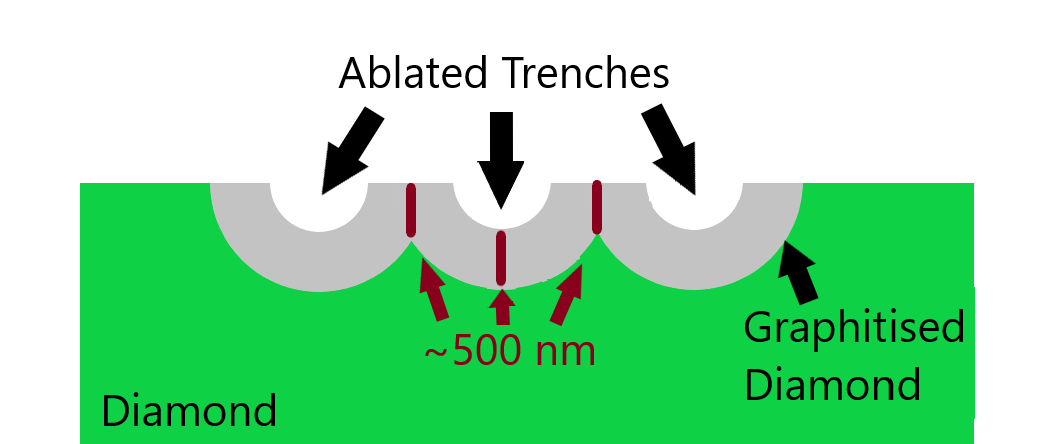
\includegraphics[width=\linewidth]{Chapter7/Figs/Raster/simple_ablation_model_2.png}
    \caption{A simple ablation model to demonstrate the approximate thickness of graphitic material.}
    \label{fig:simple_ablation_model_2}
\end{figure}

A rudimentary model of the thickness approximation is represented in figure \ref{fig:simple_ablation_model_2}. There are a few complications that must be acknowledged with such a model. First, the order in which the laser processing is performed will affect the photographitisation/thermal graphitisation process itself, with additional ablation occurring when laser treatment is applied adjacent to a point which already has a significant degree of graphitisation. This may be one of the most significant reasons as to why the profile of laser treated surface wires shows one deep topological trench, with a roughness that may then be due to the individual ablation regions. 

Second, the spacing between adjacent laser spots will naturally change the ablation regions, and surface topology, with knock on effects for the graphitised region of interest. If laser spots are kept very close together, then the semi-circles representing ablated trenches in figure \ref{fig:simple_ablation_model_2} will overlap, with a non-trivial local thickness of the graphitised region in these regions of overlap. 

Thirdly, the photographitisation process is quite dependent upon defects as the origin of sp$^{3}$ bond breaking \cite{kononenko2014-PI}, in material which contains said defects. There are multiple defects that could have formed the origin of such photo-induced graphitisation, such as at the interface between the HPHT substrate and CVD grown heavily phosphorous doped diamond film \cite{tallaire2011}, within the CVD grown layer itself due to the growth conditions used for highly phosphorus doped material \cite{grotjohn2014}, and the HPHT substrate itself due to the nitrogen content and likely high density of twinning or stacking faults \cite{Angus1992}, \cite{sumiya2015}. Hence, the origin of photographitisation is difficult to ascertain in such a substrate, and this may lead to a small amount of variance in the depth at which the sp$^{2}$ seeds are formed. The relative consistency of the topological scans demonstrated thus far indicates that despite these complications in a more precise model of the thickness of graphitised material, the ablation within the wider wires where multiple passes of laser processing has occurred is reasonably consistent. This removes the third point from relevance, as the exact positioning of the photo-induced graphitisation process need not be considered a large factor. 

While the first and second points still hold, comparison to previous work indicates that while there may be some variability in the local thickness of laser graphitised layers, the approximate thickness of 500~\si{\nano\metre} should provide a reasonable estimate of the resistivity of these layers. At minimum, there should not be any points within the laser written wires where there is a thickness substantially thinner than 500~\si{\nano\metre}, with large deviations likely to be slightly thicker than this estimate. 

\subsubsection{Graphitised Wire Testing - 14 micron width}
\label{subsubsec:graphitised_wire_testing_14}
\begin{figure}[H]
    \centering
    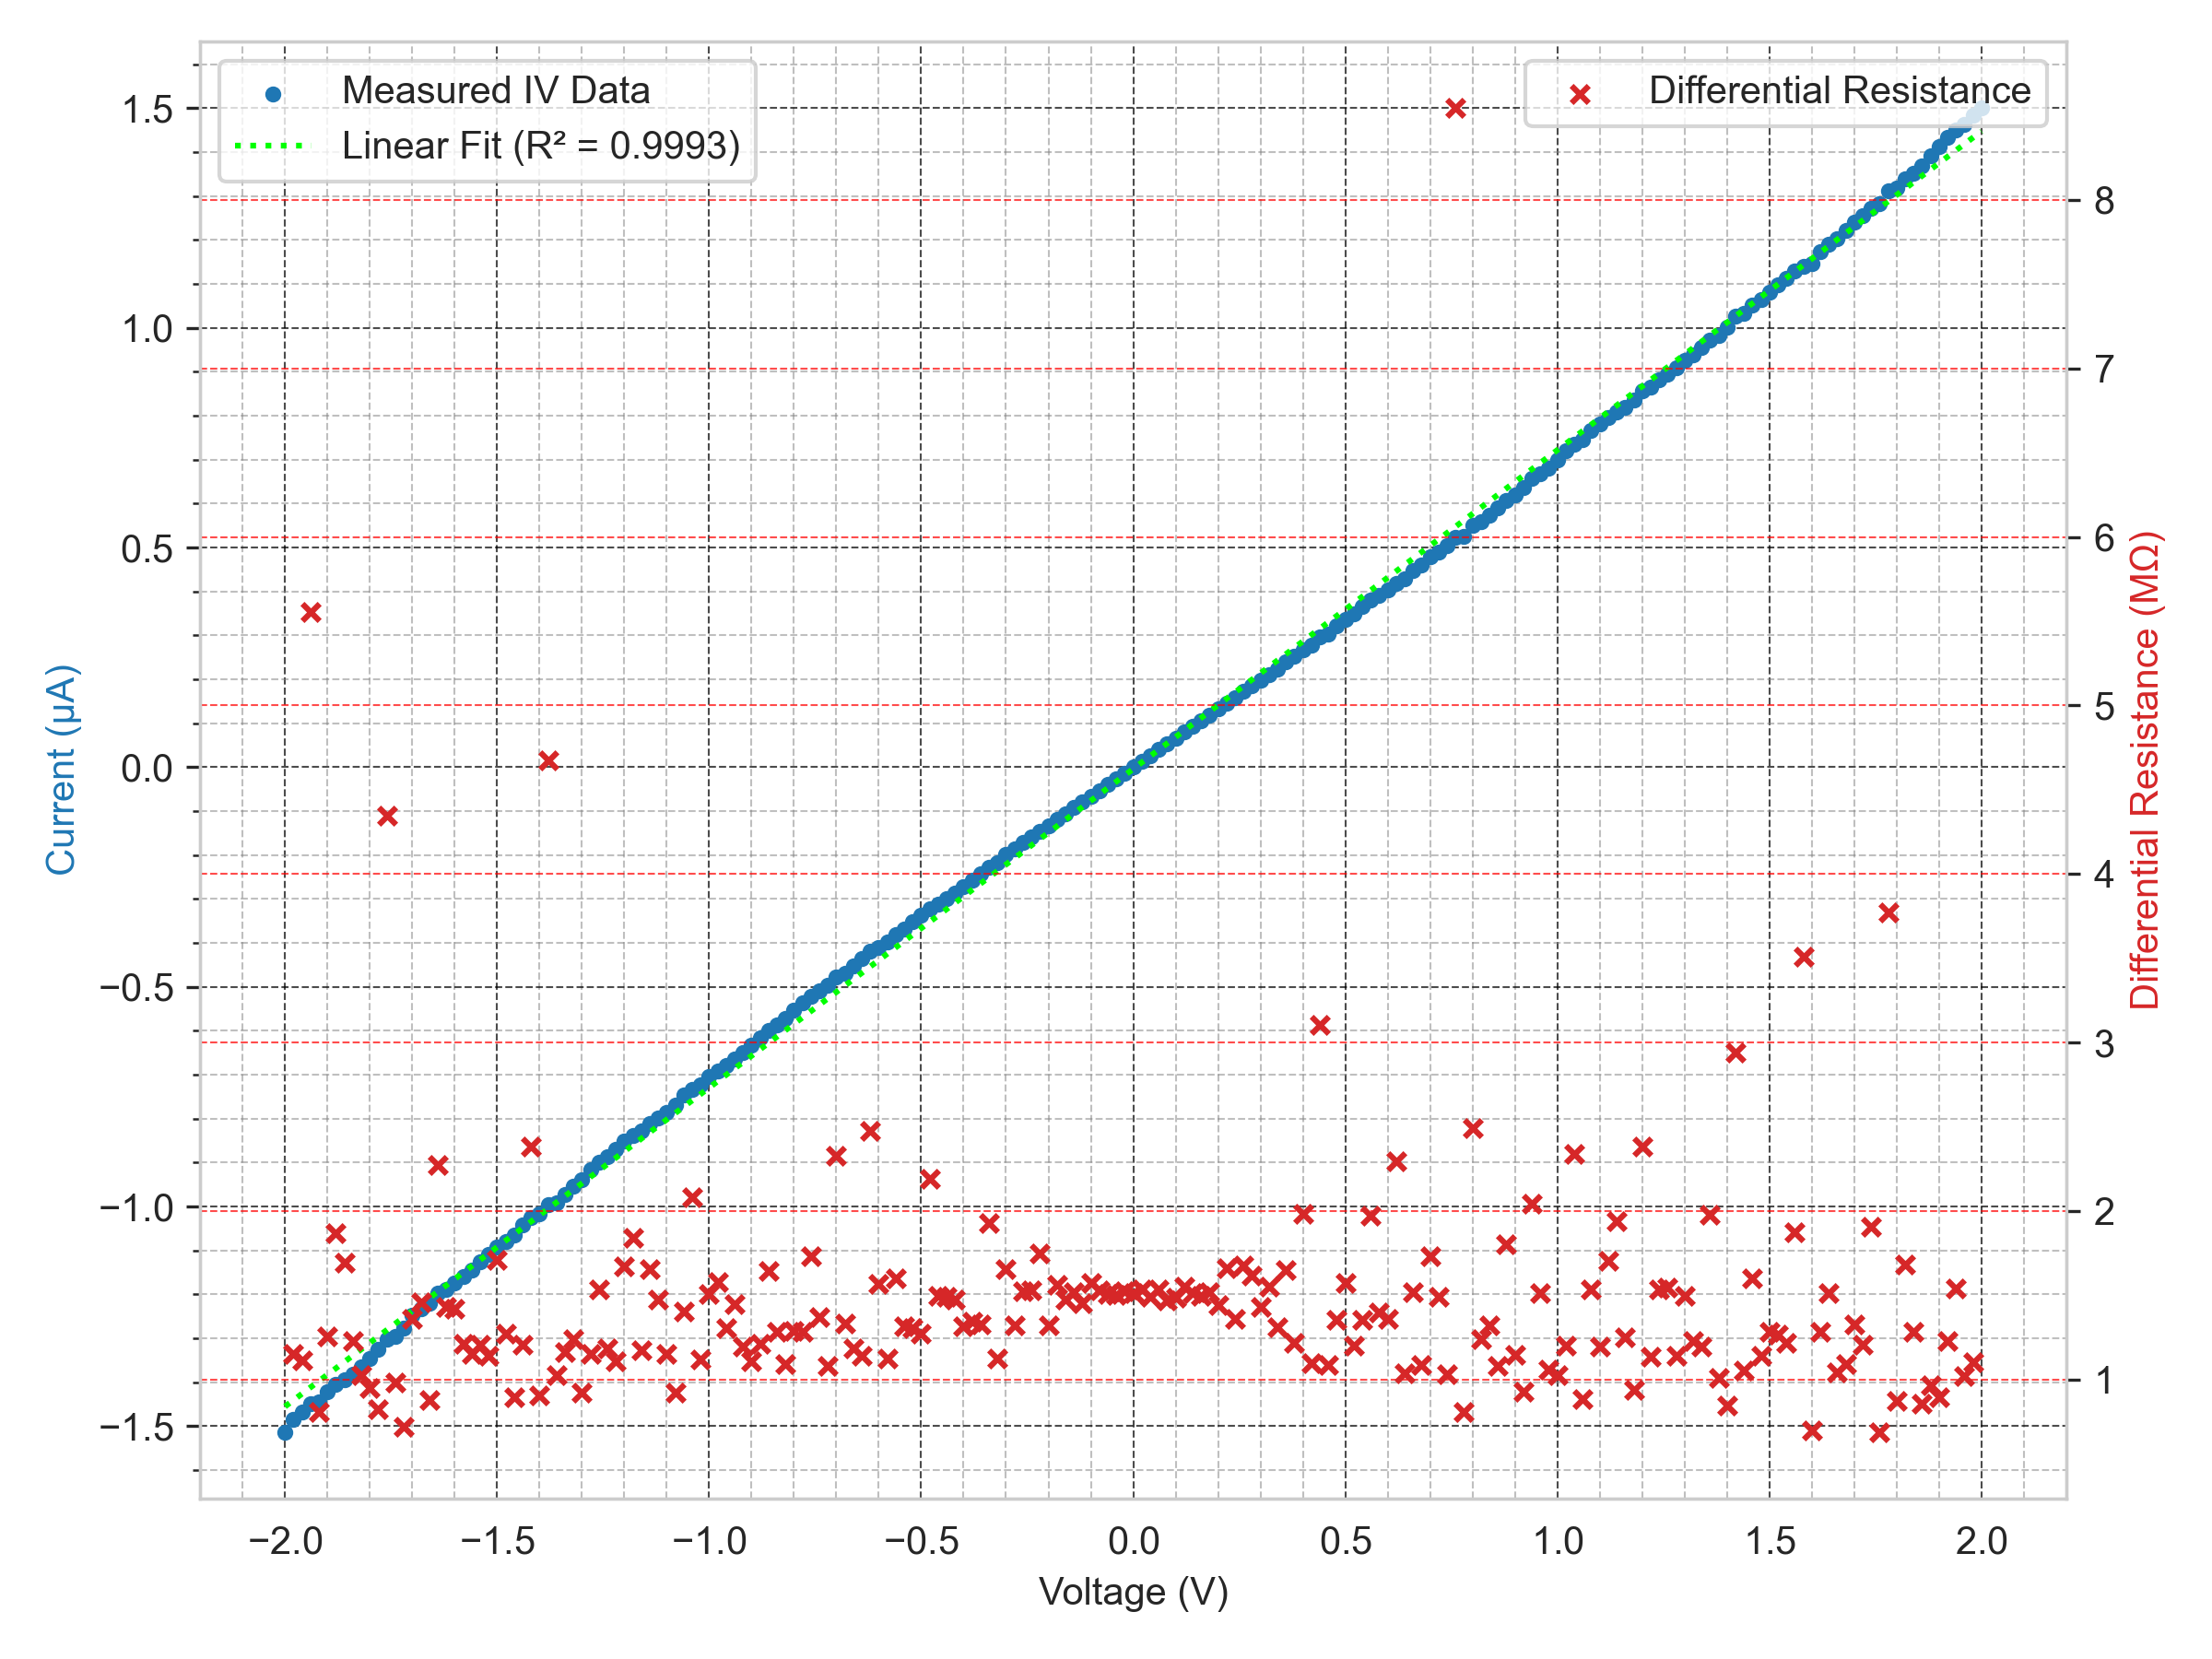
\includegraphics[width=\linewidth]{Chapter7/Figs/Raster/2V AB d.png}
    \caption{The first set of electrical measurements across the 14~\si{\micro\metre} wire structure via probe locations A and B.}
    \label{fig:2v_ab}
\end{figure}
The first set of electrical measurements were carried out between probe positions A and B as shown in figure \ref{fig:big_bone_esid}. The linear IV plot is shown in figure \ref{fig:2v_ab}, and shows a good ohmic relationship in the low voltage region of $\pm$ 2~\si{\volt} (R$^{2} = 0.9993$). This line of best fit corresponds to a measured total resistance of $1.34$~\si{\mega\ohm}. A full set of electrical measurements were taken from this starting point, increasing up to an absolute potential bias of 100~\si{\volt} applied at probe A, with probe B held at ground. Figure \ref{fig:2v_ab} also displays the differential resistance between consecutive data points, further demonstrating the ohmic quality of this wire.

\begin{figure}[H]
    \centering
    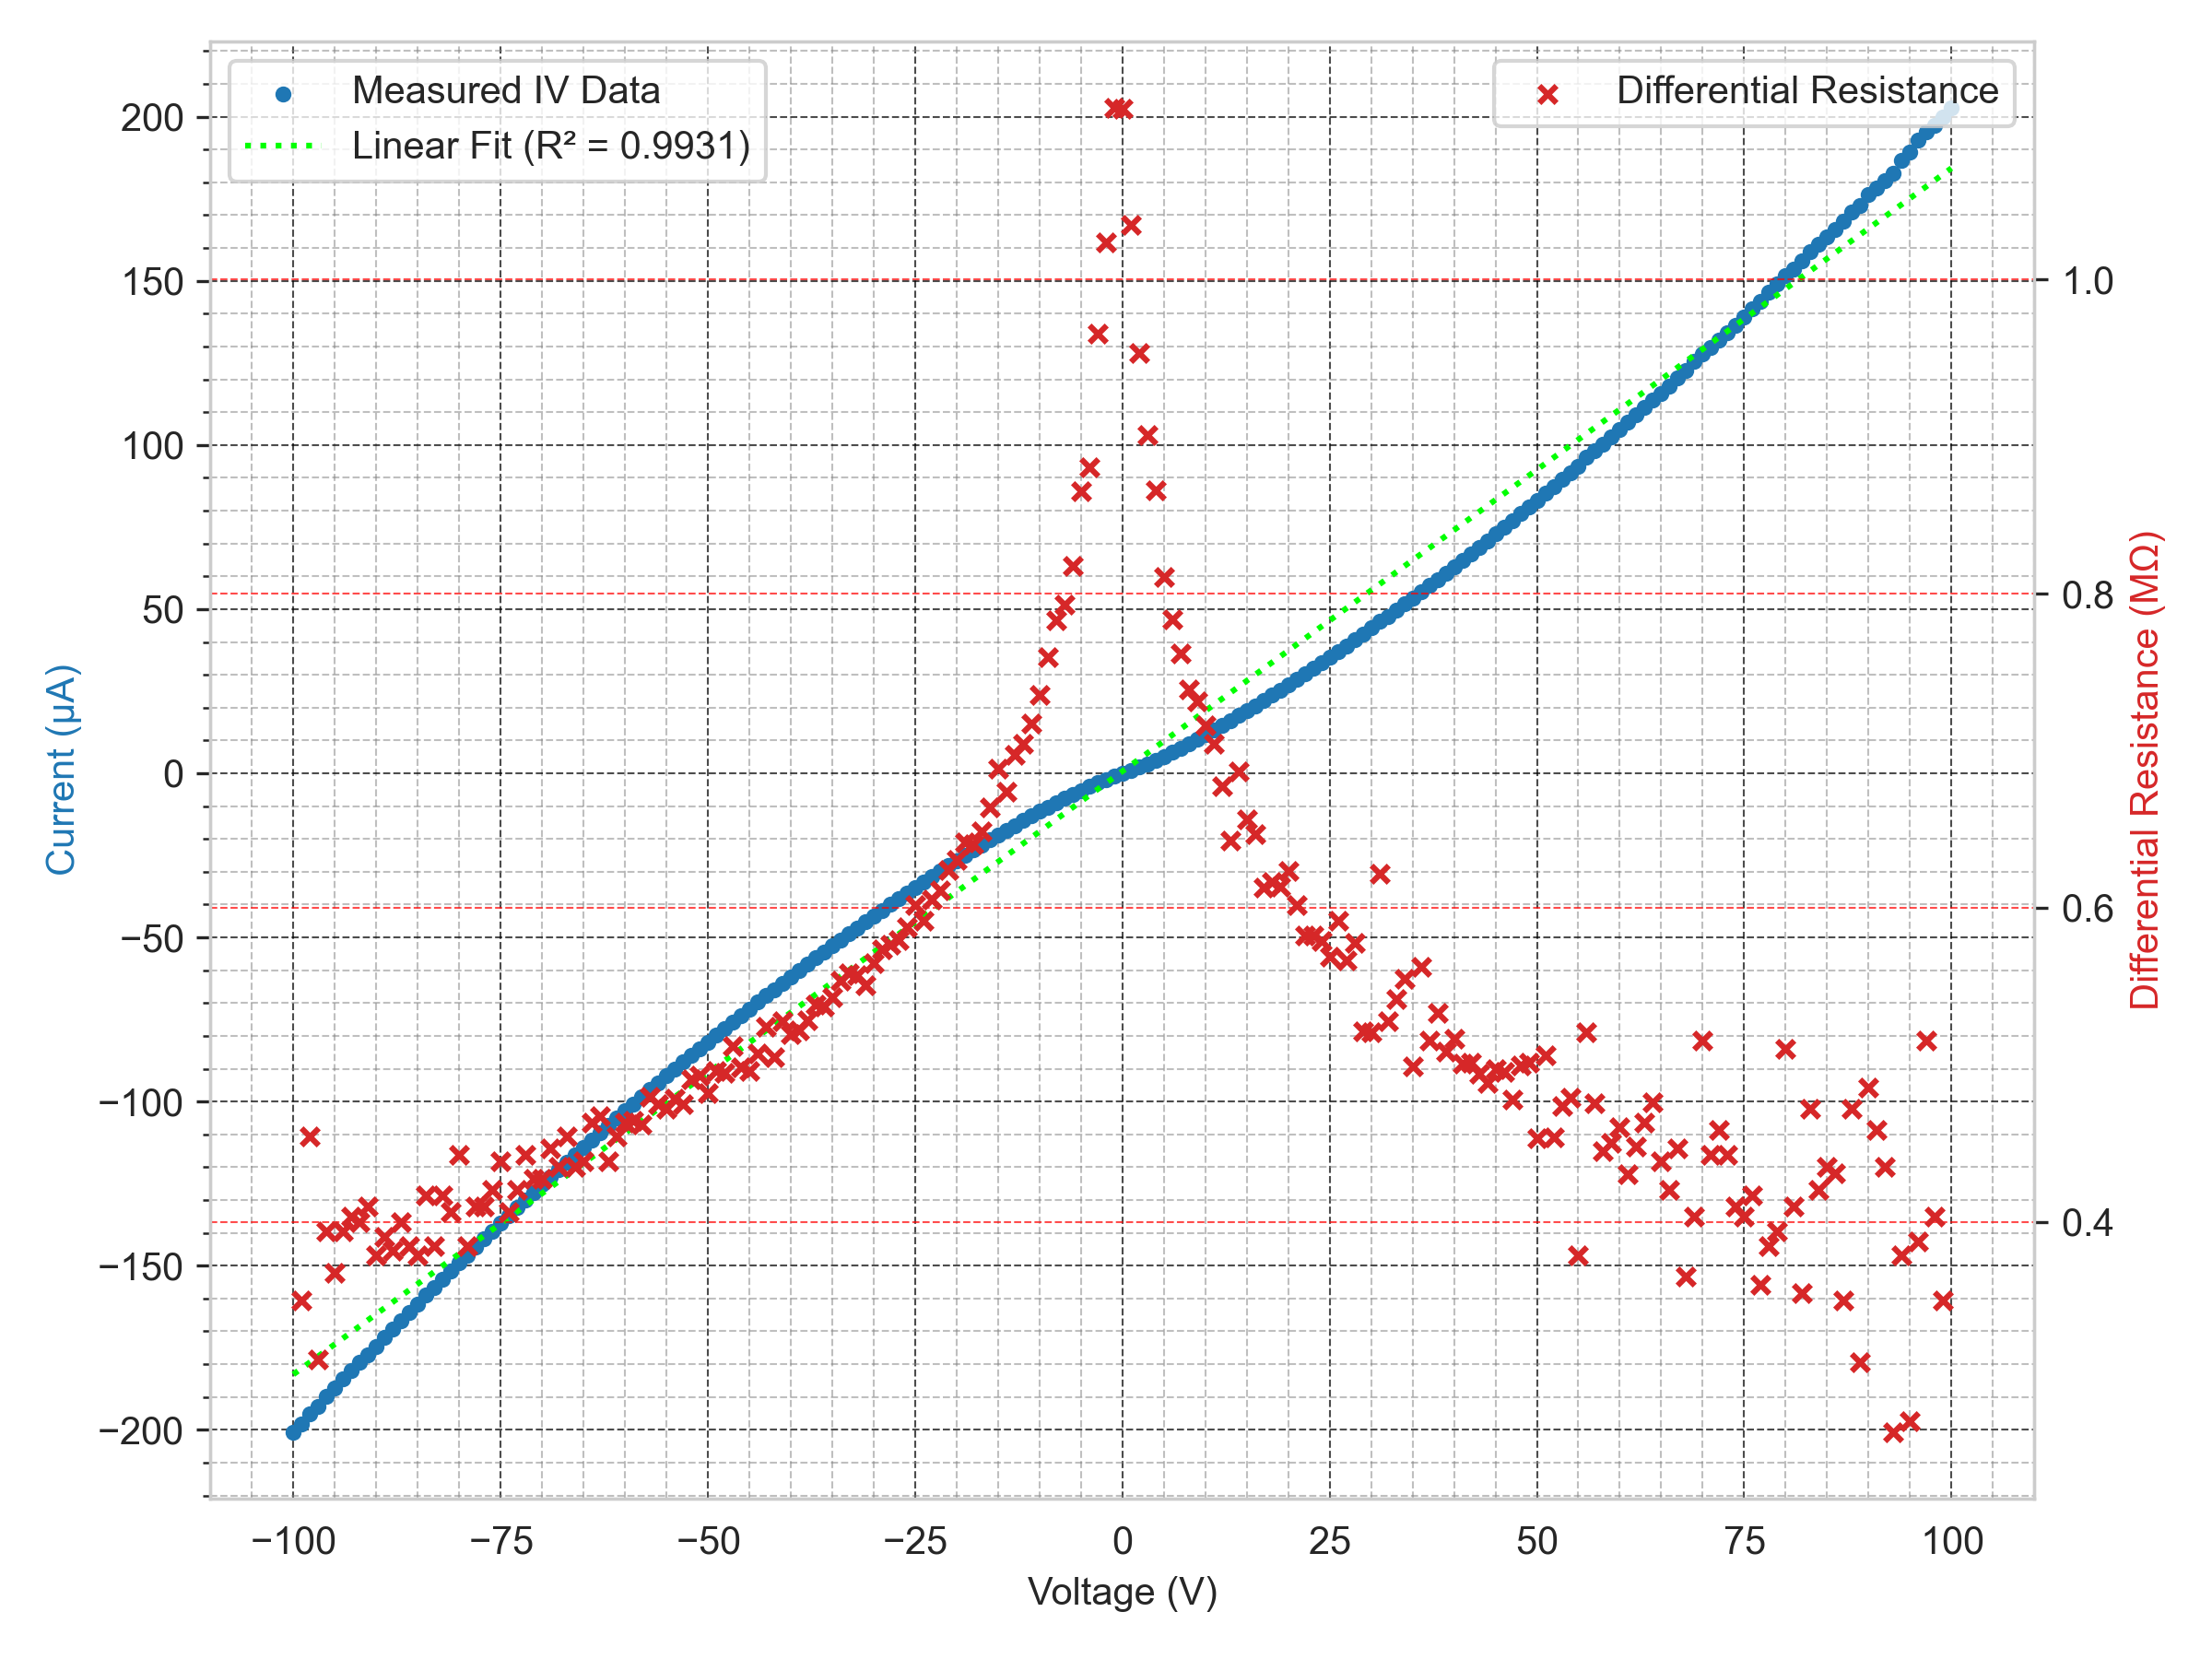
\includegraphics[width=\linewidth]{Chapter7/Figs/Raster/100V AB d.png}
    \caption{A $\pm$100~\si{\volt} set of electrical measurements across the 14~\si{\micro\metre} wire structure via probe locations A and B.}
    \label{fig:100v_ab}
\end{figure}

\begin{table}[ht]
\centering
\begin{tabular}{|c|c|c|c|c|}
\hline
Voltage (V) & Total Resistance (M$\Omega$) & Diff. in Resistance (k$\Omega$) & Absolute \% Diff. & R² \\
\hline
2  & $1.38$ & $14.9$ & 1.08\% & 0.9993 \\
5  & $1.21$ & $-19.8$ & 1.64\% & 0.9964 \\
10 & $0.992$ & $-16.1$ & 1.62\% & 0.9925 \\
20 & $0.771$ & $11.6$ & 1.50\% & 0.9930 \\
40 & $0.629$ & $6.18$ & 0.98\% & 0.9914 \\
60 & $0.589$ & $16.8$ & 2.85\% & 0.9933 \\
80 & $0.571$ & $-14.0$ & 2.45\% & 0.9937 \\
100& $0.544$ & $-5.57$ & 1.02\% & 0.9931 \\
\hline
\end{tabular}
\caption{Total resistance, difference in positive vs negative resistances, the absolute percentage difference, and total R$^{2}$ for various voltage ranges.}
\label{tab:resistance_difference_total}
\end{table}

Figure \ref{fig:100v_ab} shows the electrical characteristics when measured with a potential bias of $\pm100$~\si{\volt}. In contrast to the lower voltage range, a Schottky behaviour can be observed. The linear fit yields an R$^{2}$ value of 0.9931, and a measured total resistance for this linear fit of $0.544$~\si{\mega\ohm}. One valuable thing to consider with these characteristics is the potential for asymmetry in the measured resistance, and how this may change as the voltage range changes. To examine this briefly, table \ref{tab:resistance_difference_total} collects the calculated difference in resistance between the positive and negative regions, which may be expressed as $R_{\text{diff}} = R_{+} - R_{-}$, and also shows the percentage difference between the absolute value of $R_{\text{diff}}$ and the resistance as calculated from the full fit for the dataset $\left(\frac{\left| R_{\text{diff}} \right|}{R_{\text{total}}} \times 100\%\right)$. The results indicate that the data can be well regarded as symmetric in nature, with only minor absolute \% differences between the resistance as measured from the positive and negative voltage regions. There doesn't appear to be any clear correlation between the change in sign for $R_{\text(diff)}$ and the voltage range used, though it is also difficult to state that this is due to noise or other such error in the measurements, since the absolute \% difference changes across the voltage range used. 

The examination of symmetry will be explored further with the electrical characterisation of emitter structures, due to the possibility of one-way diodes being created through the geometric field enhancement and subsequent field effect emission. However in this case, both probes A and B are placed on what is ostensibly material containing enough graphitic phase carbon to allow for near-ohmic conductivity. The observation of an inconsistent asymmetry may indicate some change in the structure of sp$^{2}$ phase carbon under the application of electrical bias, or potentially a more exotic phase of carbon such as a diaphitic structure. This will be explored further later in this chapter.

\begin{figure}[H]
    \centering
    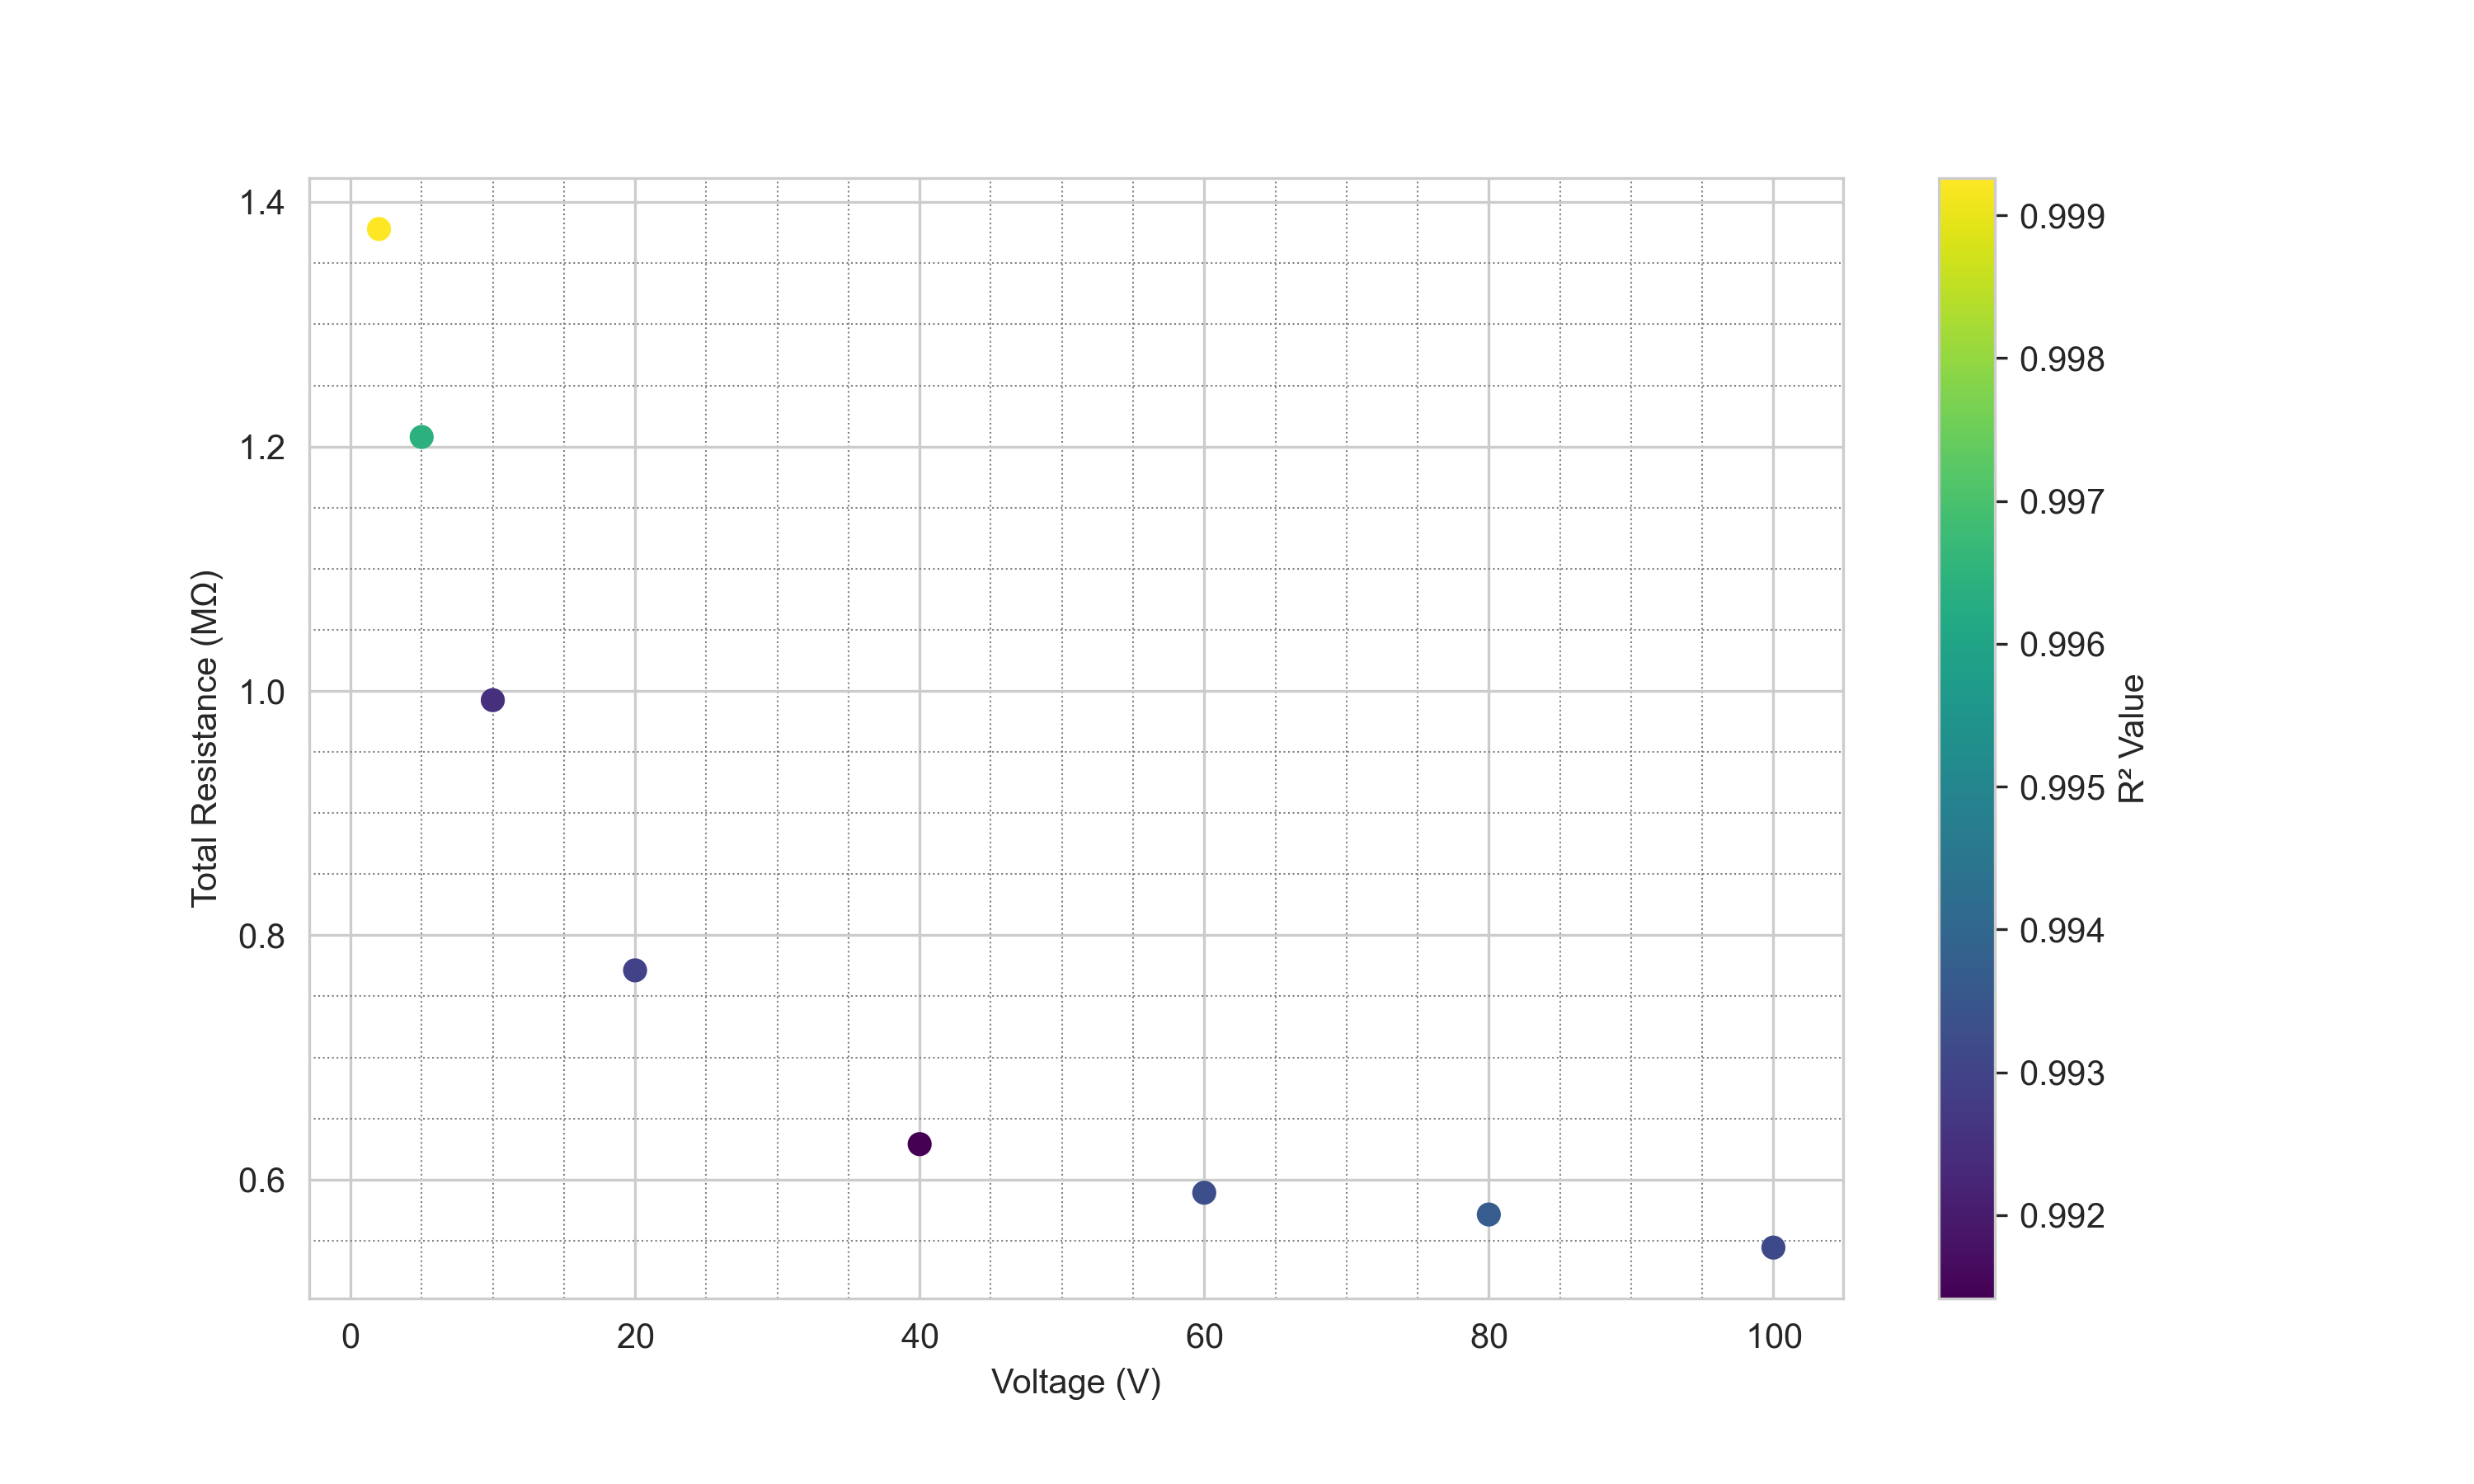
\includegraphics[width=\linewidth]{Chapter7/Figs/Raster/full_range AB.png}
    \caption{The full voltage range and their corresponding total resistances as measured across probes A and B.}
    \label{fig:full_range_ab}
\end{figure}

Figure \ref{fig:full_range_ab} displays the full range of measured total resistances based on the voltage range used. A colour scale is used to represent the changing R$^{2}$ value as the IV characteristics trend towards a Schottky-like behaviour at higher voltage ranges, deviating from the linear fit applied for the calculation of resistance.

\begin{table}[ht]
\centering
\begin{tabular}{|c|c|c|c|}
\hline
Voltage (V) & Resistivity ($\Omega$cm) & Conductivity (S/m) & Conductivity Error (S/m) \\
\hline
2 & $5.88$ & $17.0$ & $1.04$ \\
5 & $5.16$ & $19.4$ & $1.18$ \\
10 & $4.24$ & $23.6$ & $1.44$ \\
20 & $3.29$ & $30.4$ & $1.85$ \\
40 & $2.68$ & $37.2$ & $2.27$ \\
60 & $2.51$ & $39.8$ & $2.43$ \\
80 & $2.44$ & $41.0$ & $2.50$ \\
100& $2.32$ & $43.0$ & $2.62$ \\
\hline
\end{tabular}
\caption{Voltage vs. resistivity, conductivity, and a conductivity error of 6.1\% for this wire.}
\label{table:ab_resistivity_conductivity}
\end{table}

Table \ref{table:ab_resistivity_conductivity} shows the resulting resistivity and conductivity as measured across the various voltage ranges between probes A and B. Immediate comparisons could be made to typical conductivity values for graphite, which when parallel to the basal plane are typically reported to have values of 2--4$\times10^{5}$~\si{\siemens\per\metre}, and perpendicular to the basal plane are closer to $333$~\si{\siemens\per\metre} \cite{pierson1993}. The best reported conductivity here at a bias of 100~\si{\volt} is of $43.0$~\si{\siemens\per\metre}, approximately 8 times smaller than that of the perpendicular graphite conductivity value. This is a significantly higher conductivity than that of the diamond substrate itself as measured via LTLM and CTLM in chapter \ref{ch:electrical_experiments} on another sample with a heavily phosphorous doped surface layer grown under the same conditions as for this sample. However it is difficult to infer the dominant form of carbon allotrope that is present, especially when the concept of electrical percolation within composite materials is considered as in \cite{mclachlan1990}. The recent application of complex network theory to electrical conduction mechanisms in nanostructure assemblies allows for a wide range of conduction types, even in materials that at first appear to be discontinuous \cite{yao2020}. Hence, the reduced resistivity observed in laser treated diamond that contains a larger content of sp$^{2}$ bonded carbon would appear to show that despite not being a truly "graphitic" wire that acts as a metal, with conductivity similar to that of bulk graphite, enough electrically conductive material is present to allow for ohmic conductivity, albeit with a higher resistance than might be expected.

\begin{figure}[H]
    \centering
    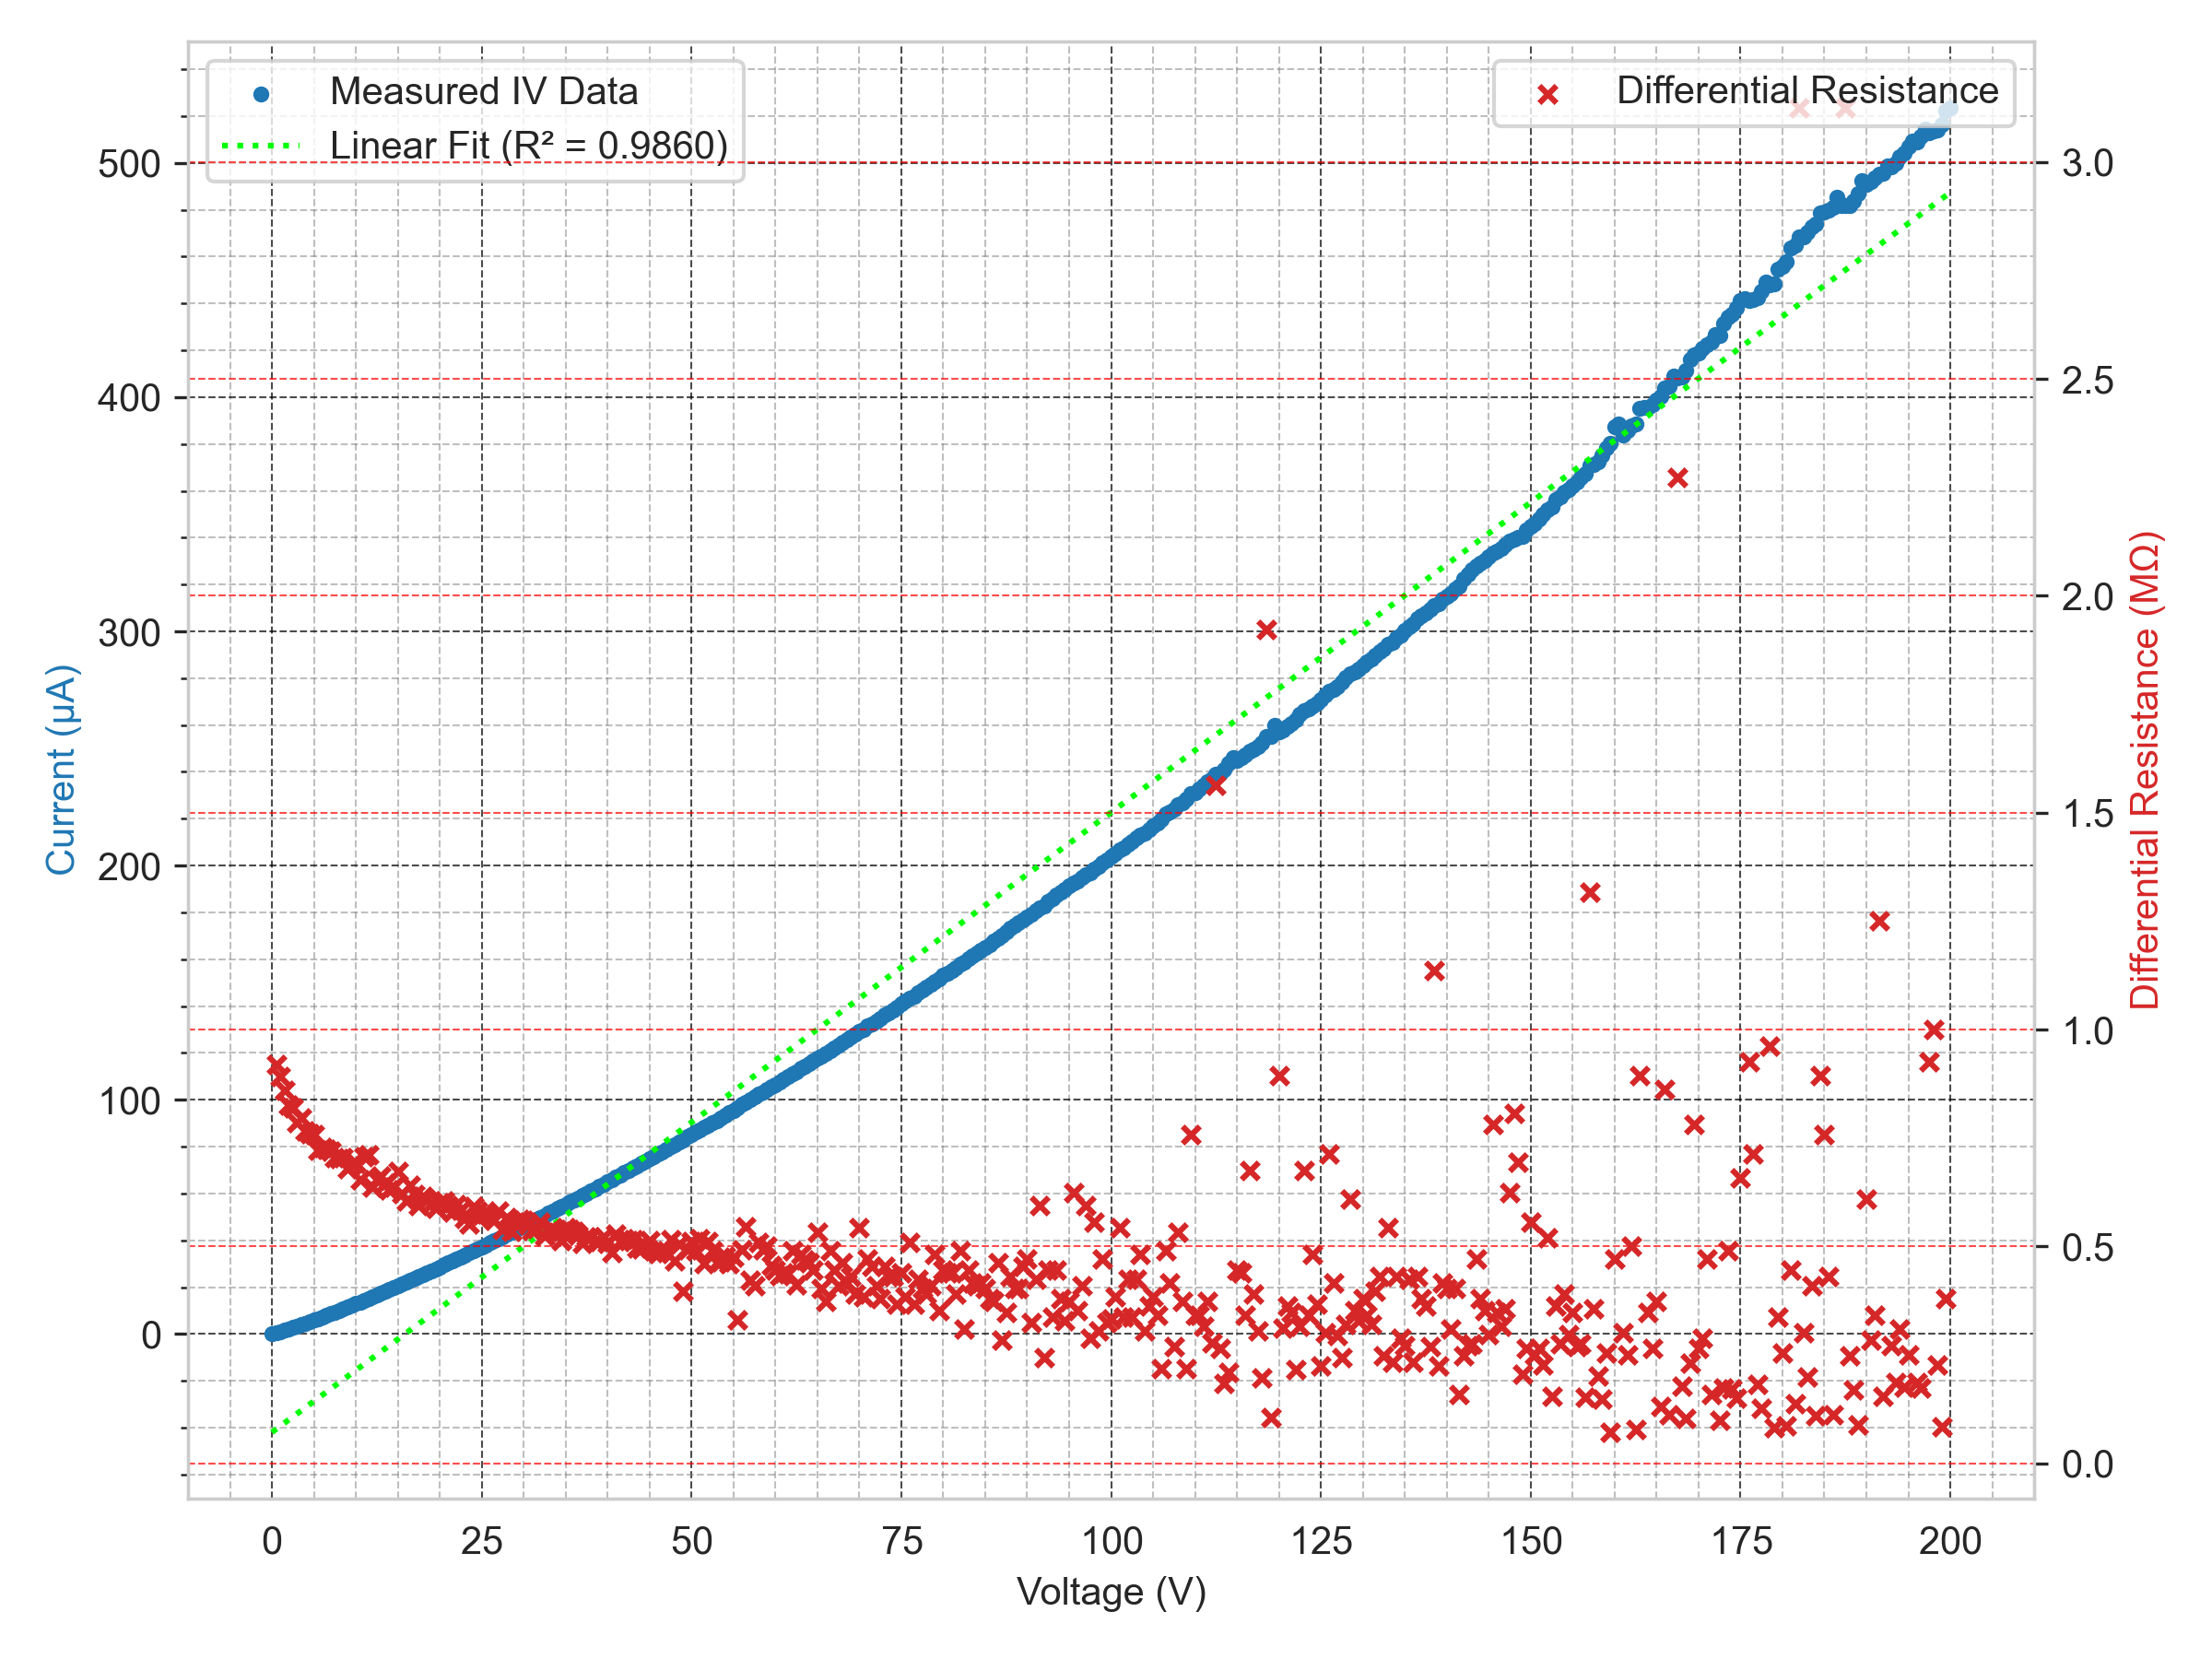
\includegraphics[width=\linewidth]{Chapter7/Figs/Raster/200V AB d.png}
    \caption{A set of electrical measurements across the 14~\si{\micro\metre} wire structure via probe locations A and B, reaching up to 200~\si{\volt}.}
    \label{fig:200v_ab}
\end{figure}

\begin{table}[ht]
\centering
\begin{tabular}{|c|c|c|c|}
\hline
Voltage (V) & Resistivity ($\Omega$cm) & Conductivity (S/m) & Conductivity Error (S/m) \\
\hline
4 & 4.06 & 24.6 & 1.50 \\
10 & 3.51 & 28.5 & 1.74 \\
20 & 3.07 & 32.6 & 1.99 \\
40 & 2.64 & 37.9 & 2.31 \\
60 & 2.38 & 42.0 & 2.56 \\
80 & 2.20 & 45.4 & 2.77 \\
100 & 2.09 & 47.8 & 2.92 \\
120 & 1.99 & 50.3 & 3.07 \\
140 & 1.89 & 52.8 & 3.22 \\
160 & 1.80 & 55.5 & 3.39 \\
180 & 1.73 & 57.9 & 3.53 \\
200 & 1.61 & 62.0 & 3.78 \\
\hline
\end{tabular}
\caption{Total voltage sweep vs. resistivity, conductivity, and a conductivity error of 6.1\% for the wire.}
\label{table:total_sweep_resistivity_conductivity}
\end{table}

Next, higher voltage testing was performed which continued the same observations as outlined in table \ref{table:ab_resistivity_conductivity}. An example of a 200~\si{\volt} sweep is shown in figure \ref{fig:200v_ab}, with a linear fit corresponding to a measured resistance of $3.78\times10^{5}$~\si{\ohm} plotted alongside the raw data. The Schottky-like behaviour continues to grow in significance at these higher voltages, with more deviation from the linear fit visible. However, the effective conductivity continues in much the same trend as before, with a conductivity of 62~\si{\siemens\per\metre} from the linear fit. This is represented in figure \ref{fig:200v_ab} by the decrease in differential resistance at higher voltages.

Table \ref{table:total_sweep_resistivity_conductivity} gives the full set of higher voltage data between probes A and B. This set of measurements was performed with fresh probe tips and a complete reset of the experimental setup, to ensure that the results were not dependent upon an unknown error related to the previous set of result. Similar to the previous measurements, the conductivity at a bias of 10~\si{\volt} was around $28.5\pm1.7$~\si{\siemens\per\metre}. One notable difference with these measurements is the setting of the ground probe to a negative bias, rather than holding it at ground. This allowed for a wider range of potential biases to be explored with the electrical probe station, but prevented the previous estimation of asymmetrical differences in absolute current values for negative vs positive electrical biases.

\subsubsection{Graphitised Wire Testing - 10 microns}
\label{subsubsec:graphitised_wire_testing_10}
In the previous section, the calculation of effective conductivity for the large (14~\si{\micro\metre}) laser processed wire is set out as for the measurements taken between probe locations A and B. Further measurements were taken at probe locations 1--4, following the electrical measurements of A--B. One small detail which was noticed during the testing of A--B was that following multiple voltage sweeps at higher potential differences, the observed conductivity appeared to decrease marginally across multiple sweeps. However, testing the following day was able to achieve similar results to that set out in table \ref{table:ab_resistivity_conductivity_error}. Regardless, it is worth examining the measurements between probe locations 1-4 and 2-3 separately, as these wires were otherwise untested in the previous conductivity measurements between probes A and B. They also have a different wire thickness of 10~\si{\micro\metre}, and so it may be natural to expect a higher resistivity. The comparative values of the wires are $3.57\times10^{-8}$~\si{\metre} for the 10~\si{\micro\metre} wires and $4.27\times10^{-8}$~\si{\metre} for the 14~\si{\micro\metre} wire. Hence if the wires do indeed follow the trivial calculation of resistivity using an estimated thickness of 500~\si{\nano\metre}, it is expected that these thinner wires will show a conductivity that is approximately 16\% lower than that of the 14~\si{\micro\metre} wires.

\begin{figure}[H]
    \centering
    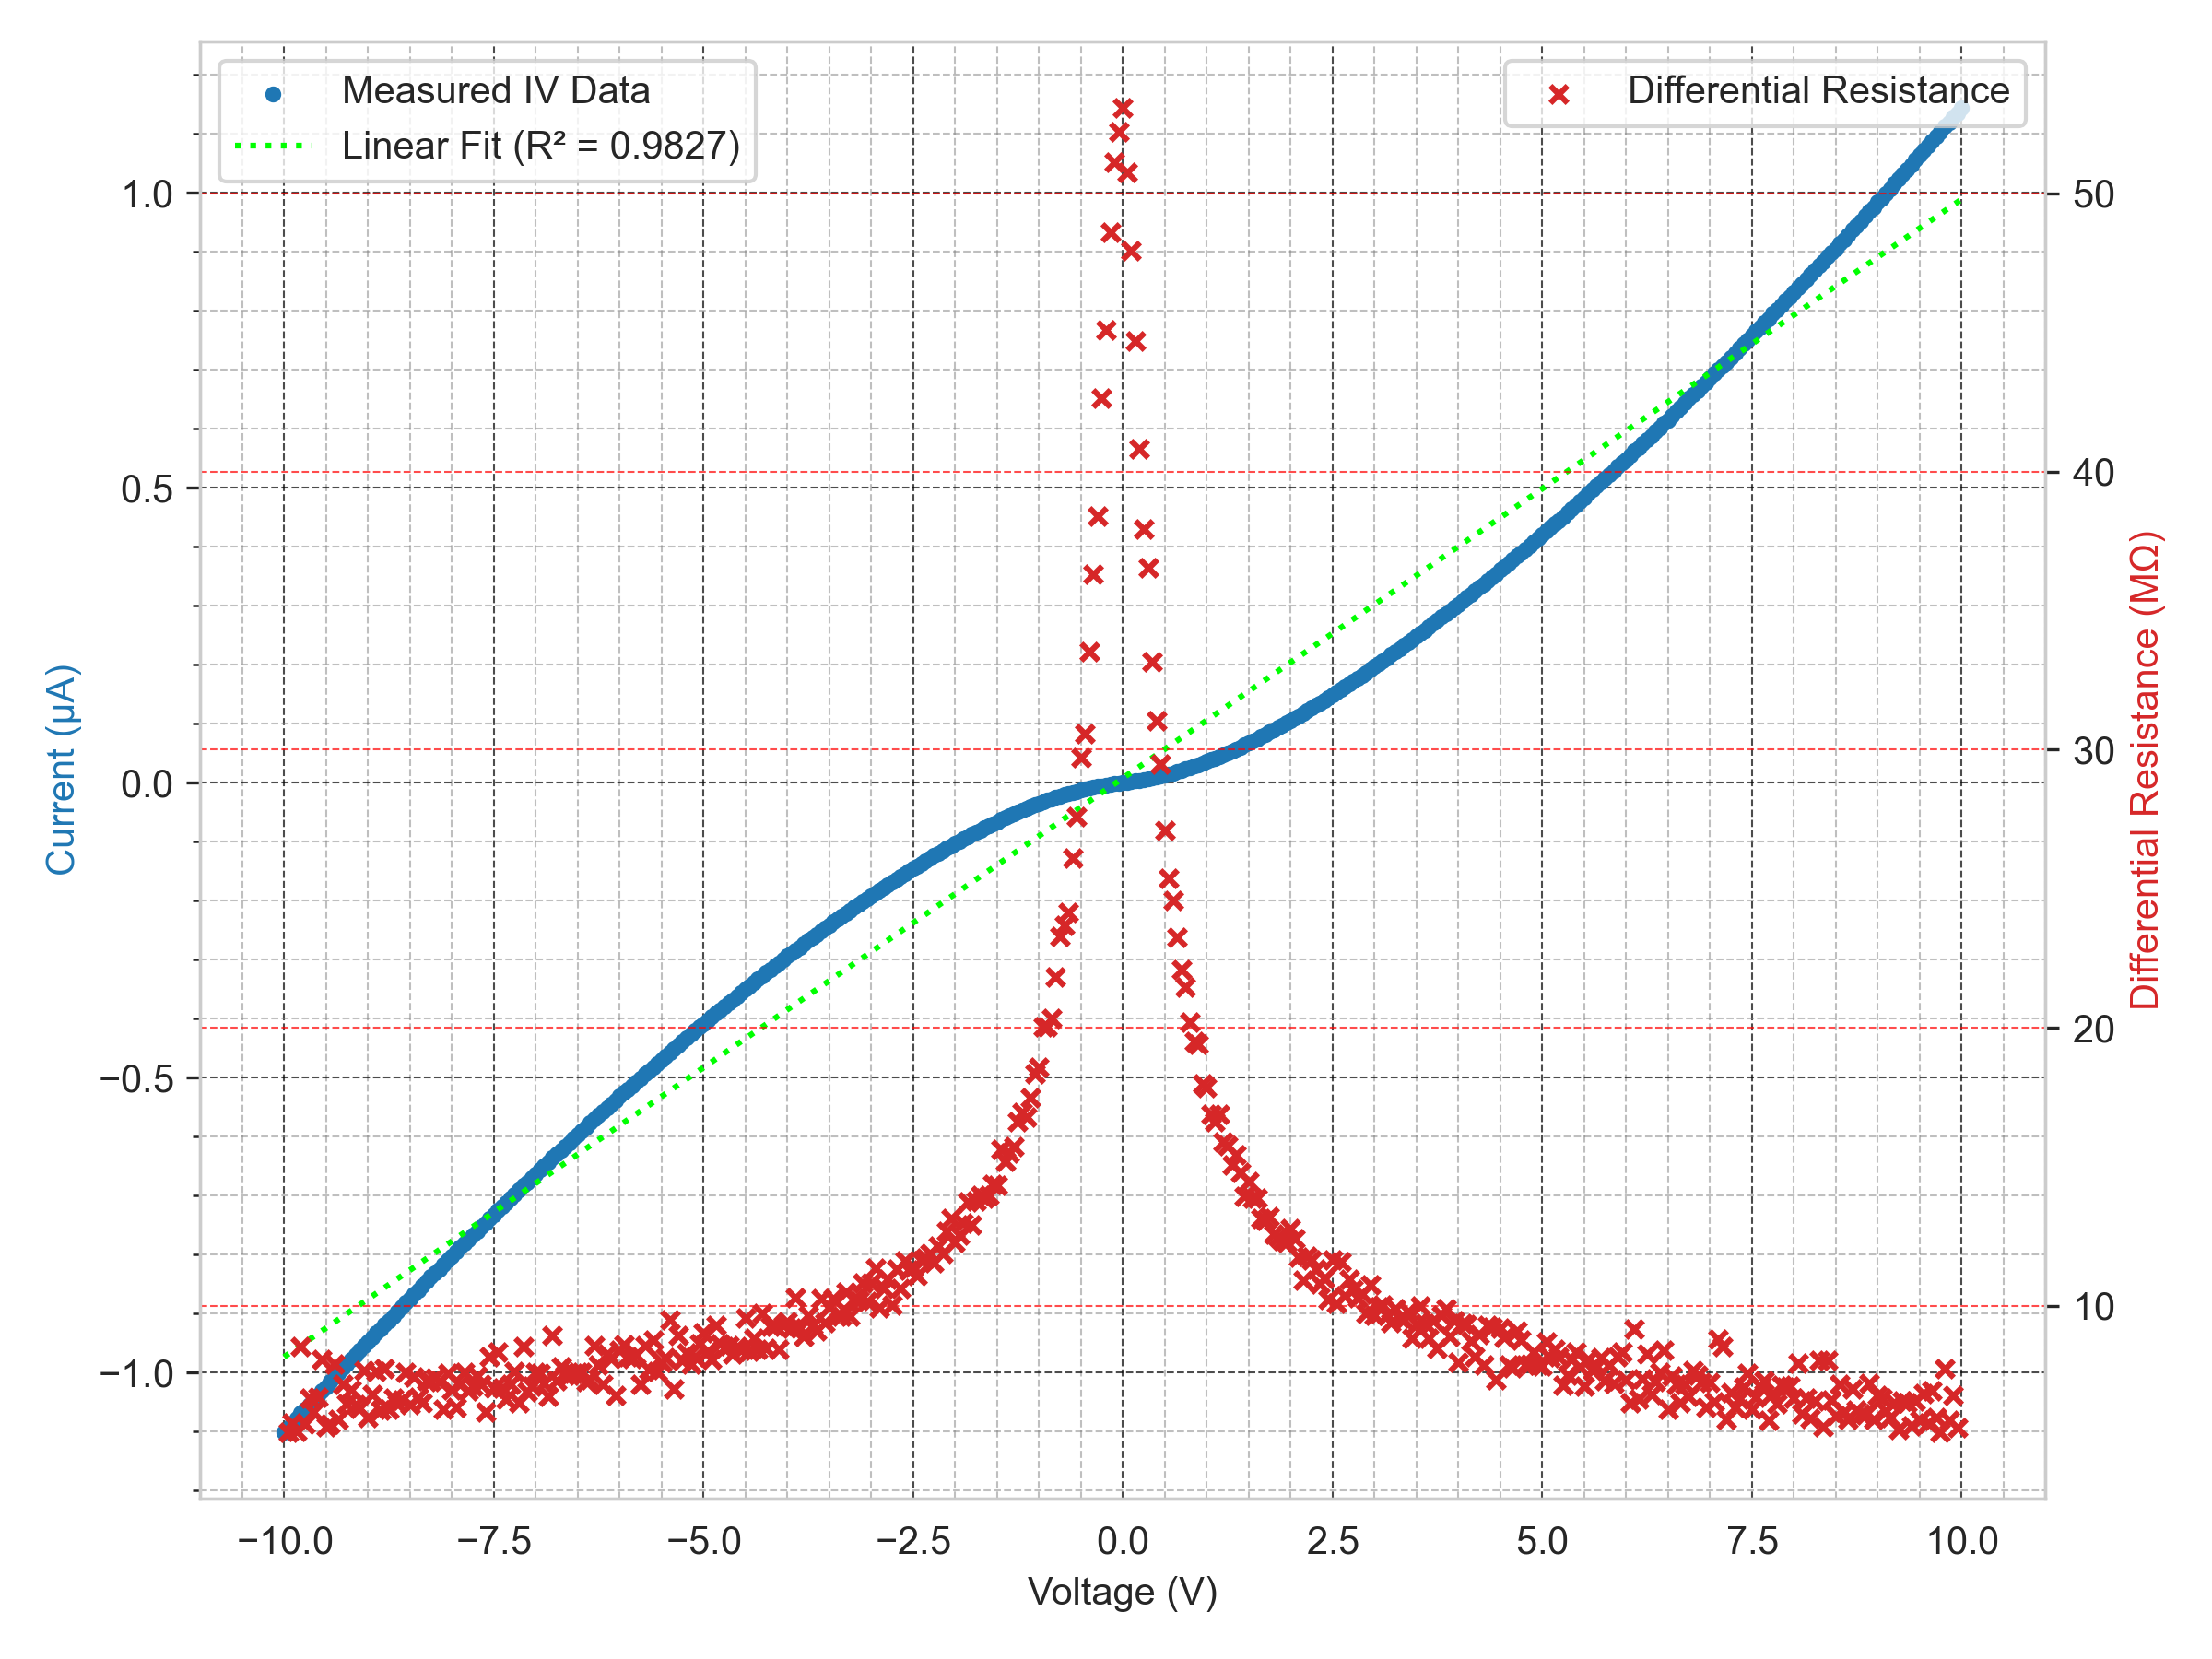
\includegraphics[width=\linewidth]{Chapter7/Figs/Raster/10V 13 d.png}
    \caption{The first electrical characteristics between probe positions 1 and 3.}
    \label{fig:10v_13}
\end{figure}

Figure \ref{fig:10v_13} shows the first measured IV characteristics of the 10~\si{\micro\metre} wire between probe positions 1 and 3. Of particular importance is the reduced absolute current relative to the thicker wire measurements, and also the clear Schottky behaviour, even given the lower bias range applied in this case. It was unclear initially if this behaviour was due to the wire itself at this stage in the experimental process. The differential resistance as plotted reflects this rise in Schottky behaviour at low voltages.

\begin{table}[ht]
\centering
\begin{tabular}{|c|c|c|c|}
\hline
Voltage (V) & Resistivity ($\Omega$m) & Conductivity (S/m) & Conductivity Error (S/m) \\
\hline
2 & $0.796$ & $1.25$ & $0.0895$ \\
10 & $0.364$ & $2.75$ & $0.196$ \\
\hline
\end{tabular}
\caption{Resistivity, conductivity, and errors for the wire between probes 1 and 3.}
\label{table:13_resistivity_conductivity_updated}
\end{table}

Table \ref{table:13_resistivity_conductivity_updated} provides a summary of the relevant conductivity data for the laser written wire between probe positions 1 and 3. The 10~\si{\volt} conductivity of approximately $2.75\pm0.20$~\si{\micro\metre} is significantly lower than the final 14~\si{\micro\metre} value of $28.5\pm1.7$~\si{\siemens\per\metre}.

\begin{figure}[H]
    \centering
    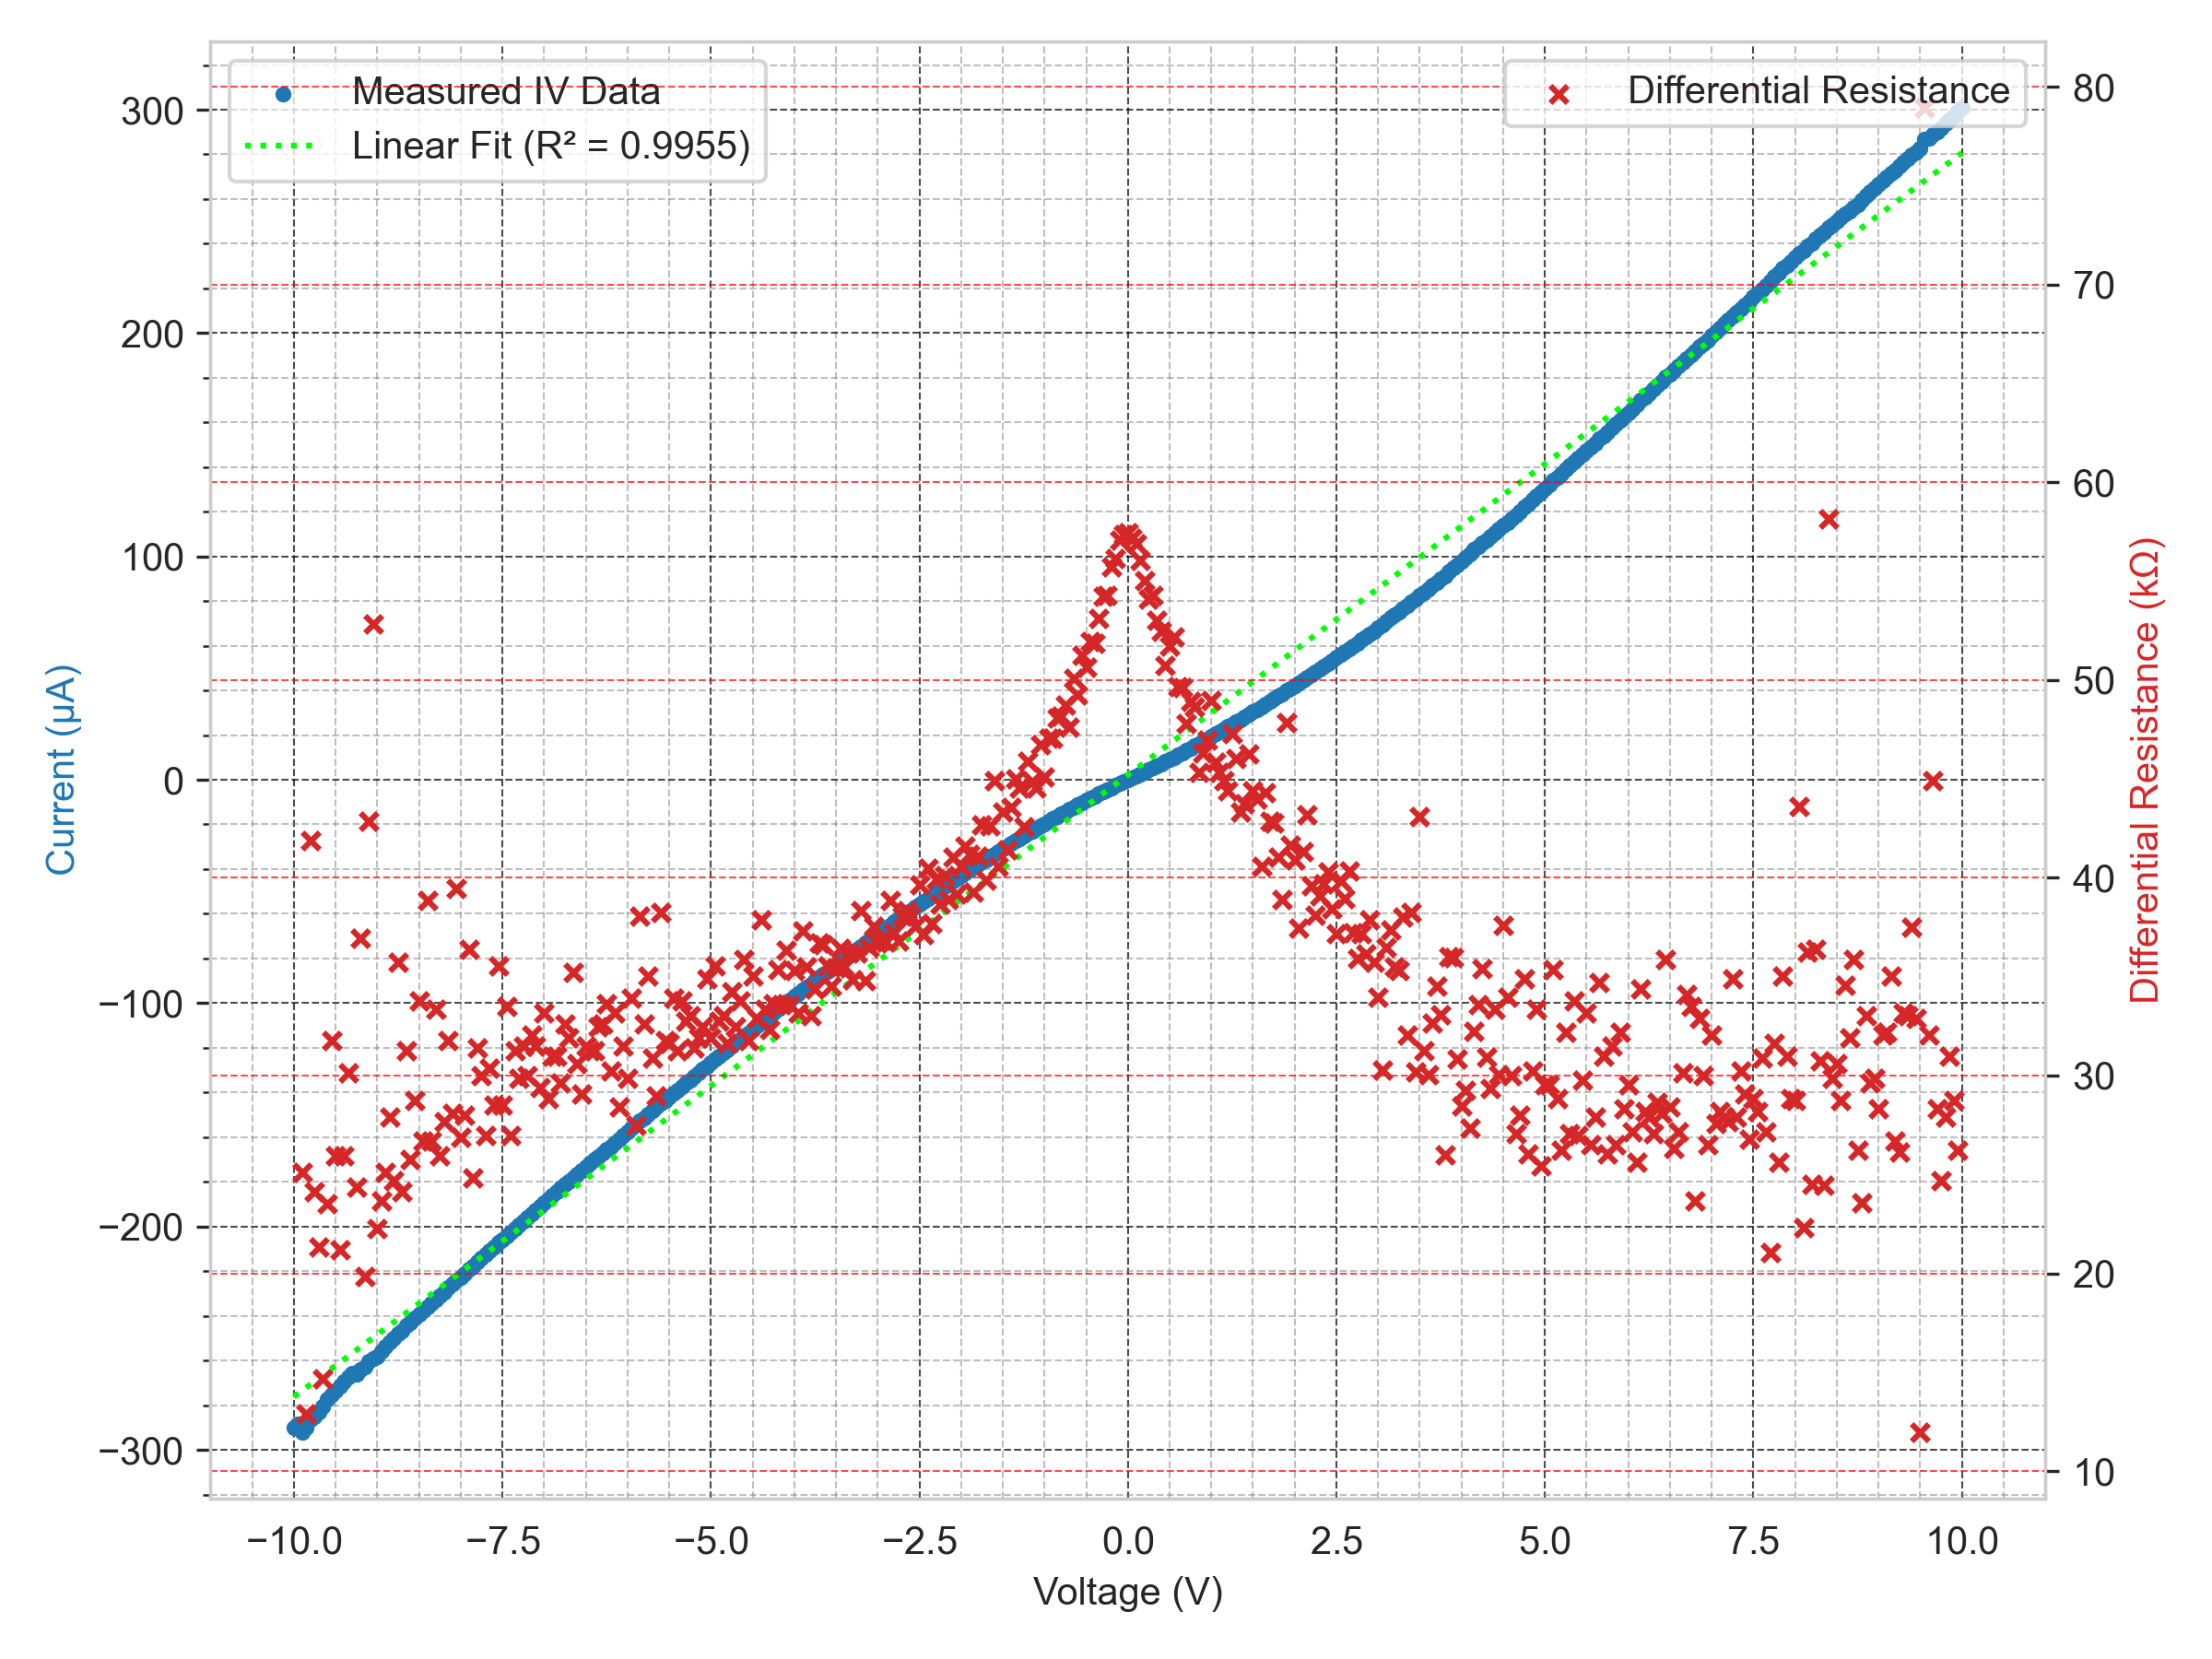
\includegraphics[width=\linewidth]{Chapter7/Figs/Raster/10V 24 d.png}
    \caption{The average electrical characteristics between probe positions 2 and 4.}
    \label{fig:10v_24}
\end{figure}

In figure \ref{fig:10v_24}, the IV measurements between probe positions 2 and 4 are plotted. This wire showed a significant jump in absolute current measurements, with the peak current reaching approximately $300$~\si{\micro\ampere}, in stark contrast to the previous measurements on both the comparable 1-3 wire and also the measurements across the 14~\si{\micro\metre}. The associated differential resistance is similarly lower by a few orders of magnitude.

\begin{table}[ht]
\centering
\begin{tabular}{|c|c|c|c|}
\hline
Voltage (V) & Resistivity ($\Omega$cm) & Conductivity (S/m) & Conductivity Error (S/m) \\
\hline
2 & 0.203 & 492 & 35.1 \\
10 & 0.128 & 780 & 55.7 \\
\hline
\end{tabular}
\caption{Resistivity, conductivity, and errors for the wire between probes 2 and 4.}
\label{table:24_resistivity_conductivity_updated}
\end{table}

In the same style as for the previous table of results for the wire between probes 1 and 3, table \ref{table:24_resistivity_conductivity_updated} shows the conductivity data for the 10~\si{\micro\metre} wire between probes 2 and 4. At 10~\si{\volt} the conductivity of this wire was measured to be approximately $780\pm1.3$~\si{\siemens\per\metre}, a factor of 284 increase in conductivity over the previous wire. This is also markedly higher than that of the 14~\si{\micro\metre} wire, with a factor of 27 increase in conductivity (for conductivity taken at 10~\si{\volt} in the 14~\si{\micro\metre} wire).

Following these results, it was apparent that repetition of the electrical characterisation was a necessity, as the drastic change in conductivity between different probe locations indicated that there may be some issues with making direct contact to the as processed laser written wires. Hence, the experimental procedure was repeated, with fresh probe tips and great care to ensure that the probe locations were as centrally located as physically possible to maximise the contacts formed. Several measurements performed with all 4 possible combinations of probe locations indicated that probe 3 in particular was the issue with the previous measurements.

\begin{figure}[H]
    \centering
    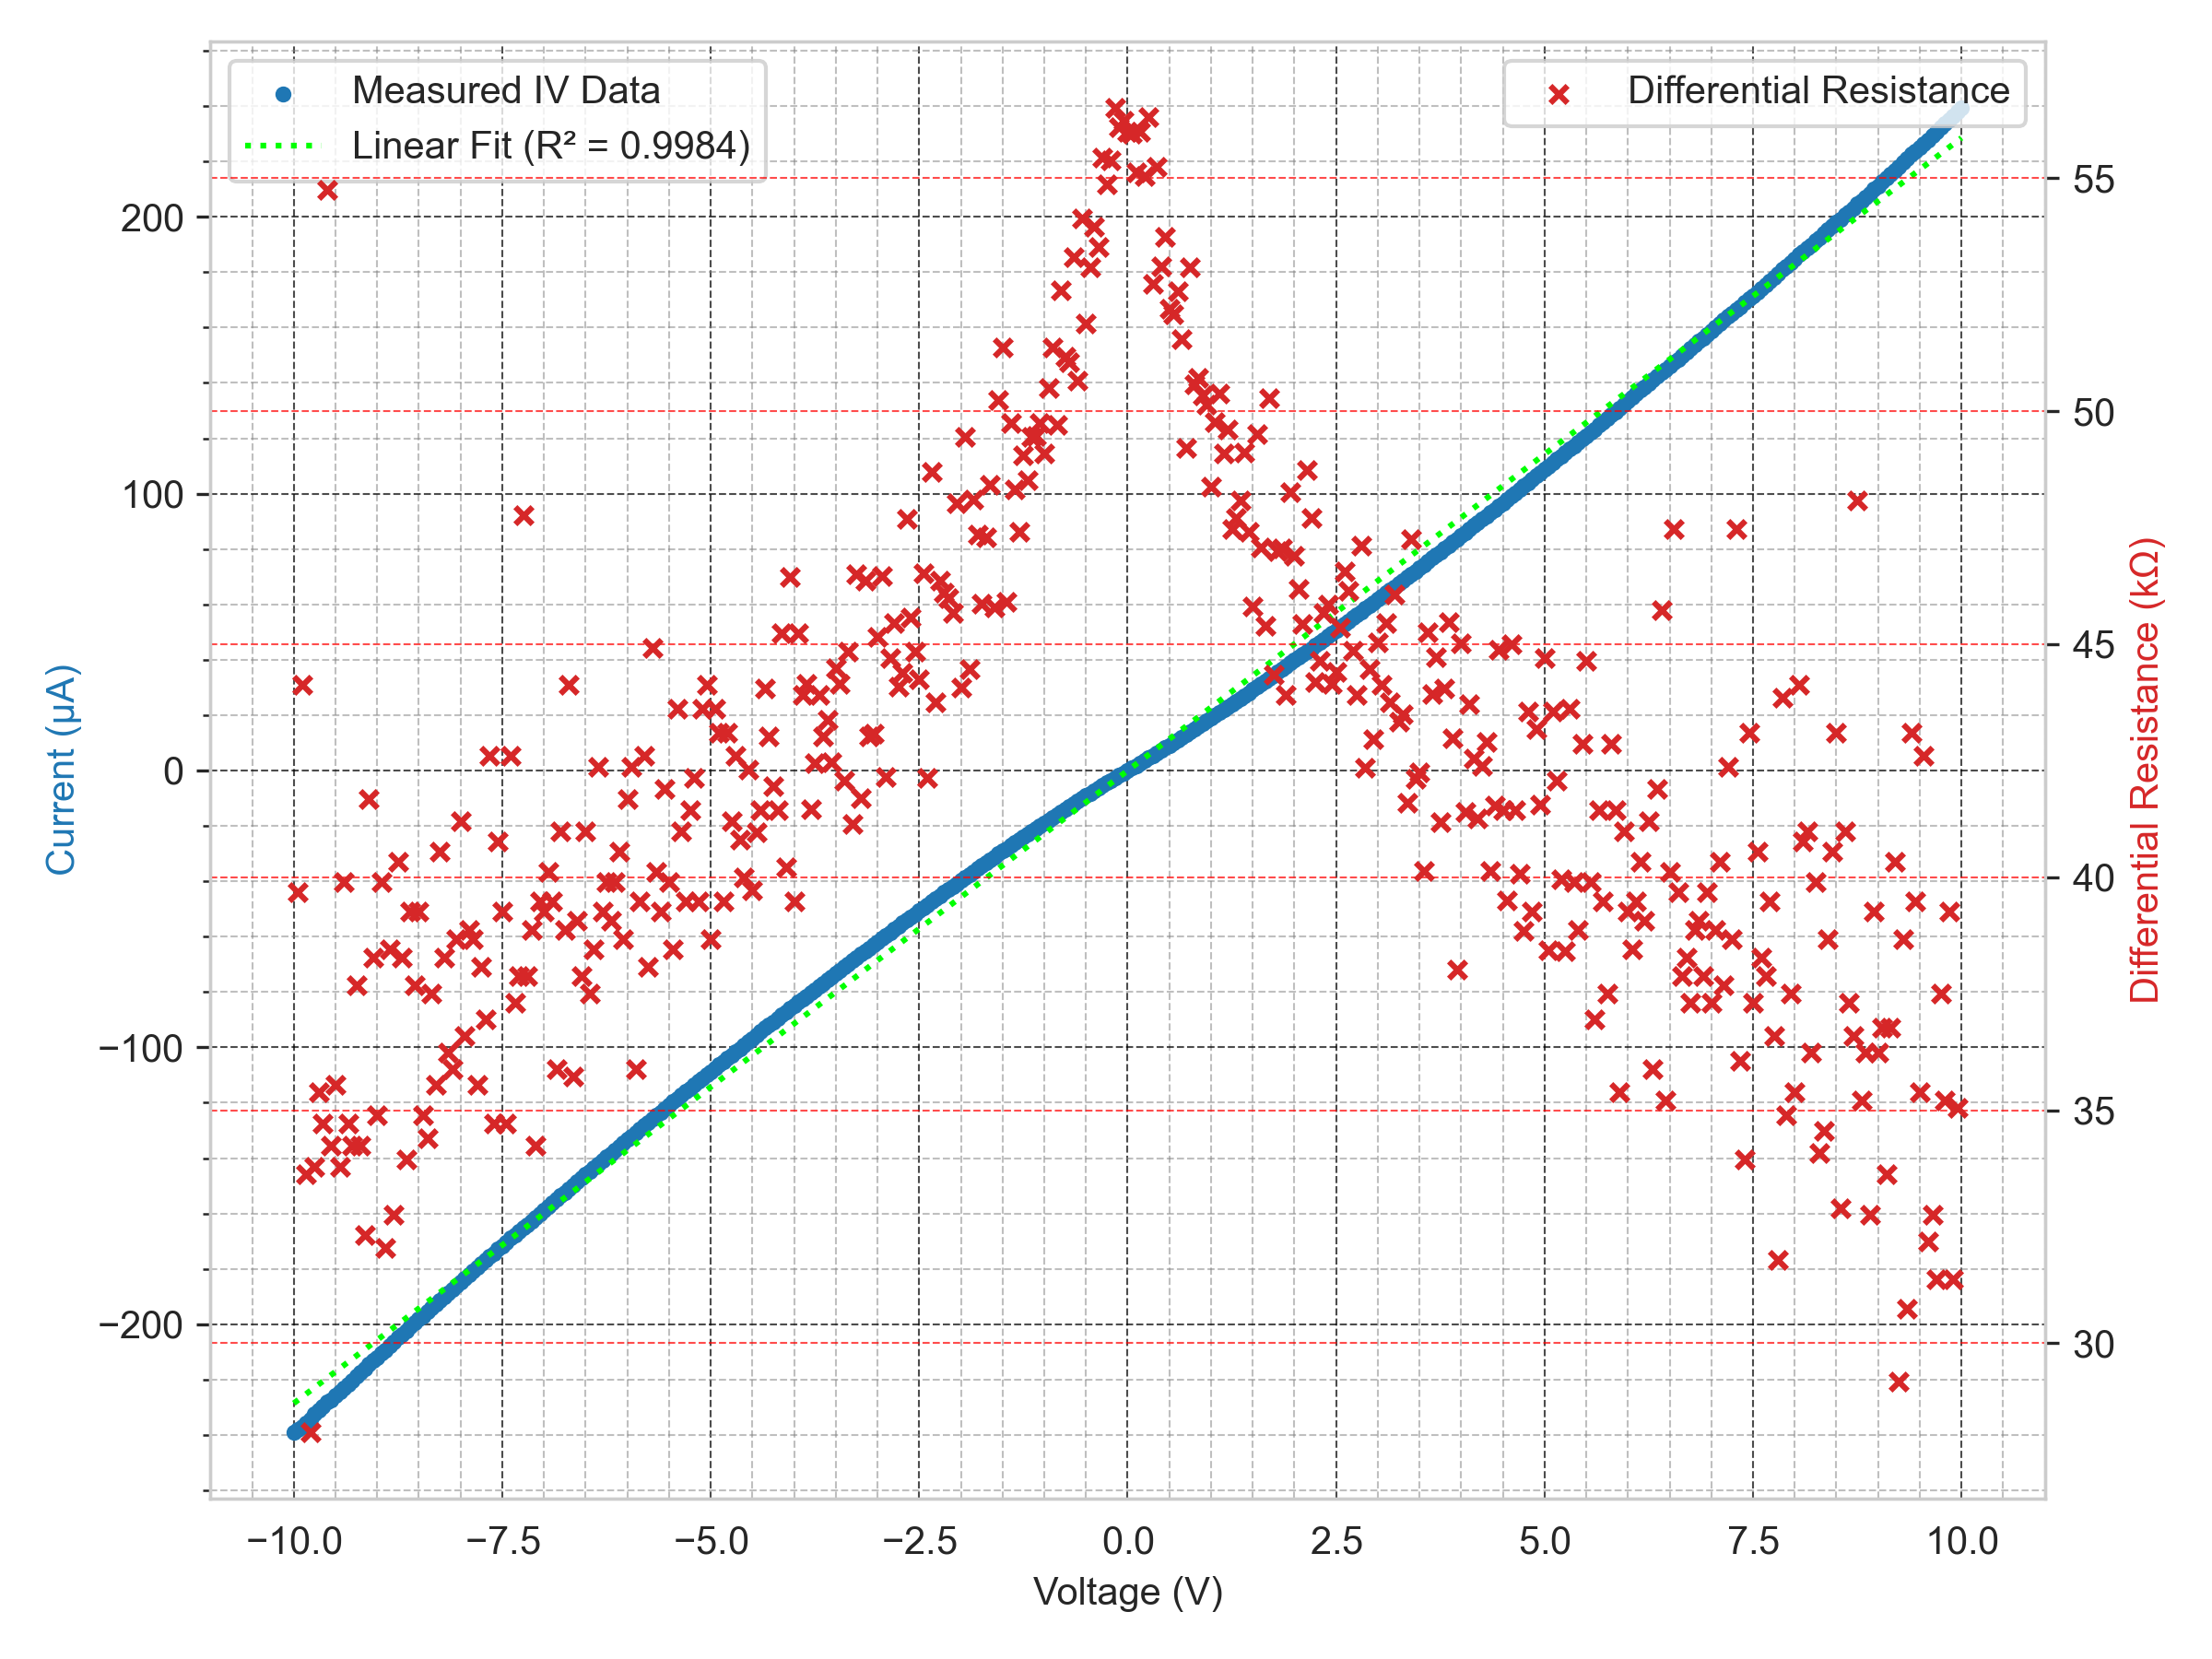
\includegraphics[width=\linewidth]{Chapter7/Figs/Raster/10V 13 replaced d.png}
    \caption{The average electrical characteristics between probe positions 1 and 3 - repeated.}
    \label{fig:10v_13_replaced}
\end{figure}

Figure \ref{fig:10v_13_replaced} shows the results of repeating this experiment with fresh probe tips and having had another standard solvent clean prior to making contact. The characteristics when contrasted to the previous data shown in figure \ref{fig:10v_13} are significantly more ohmic in nature, with the linear fit of R$^{2}$ value 0.9984 vs the previous fit of 0.9827 providing some quantification of this trend. As for 

\begin{table}[ht]
\centering
\begin{tabular}{|c|c|c|c|}
\hline
Voltage (V) & Resistivity ($\Omega$cm) & Conductivity (S/m) & Conductivity Error (S/m) \\
\hline
2 & 0.223 & 449 & 32.1 \\
10 & 0.156 & 640 & 45.7 \\
\hline
\end{tabular}
\caption{Resistivity, conductivity, and errors for the wire between probes 1 and 3 - repeated.}
\label{table:13_resistivity_conductivity_replaced}
\end{table}

The summary of further electrical measurements between probes 1 and 3 is given in table \ref{table:13_resistivity_conductivity_replaced}. Measurements between all 4 replaced probes were performed to confirm that none of the probes had a defective contact in this experimental setup, and the wire between positions 2 and 4 showed a similar conductivity to the previous results, at $749\pm53.5$~\si{\siemens\per\metre}. Further to this, a final complete replacement of electrical probes was performed to verify the order of magnitude of current being reported here, and this was in agreement. Therefore, it was concluded that the contacts in this setup were no longer the cause of any discrepancy between the measured wire conductivities. 

\subsubsection{Graphitised Wire Testing - 10 and 14 microns}
\label{subsubsec:graphitised_wire_testing_both}
In the previous two sections, the experiments performed on the wire testing structure as shown in figure \ref{fig:big_bone_esid} were used to establish the observed electrical conductivities of the 10 and 14~\si{\micro\metre} wires. Several further sets of measurements were taken across the structure, as previously alluded to in the verification that the original contact formed by probe 3 was relatively poor compared to the other 3 points of electrical contact. While the measurements across the full span of the structure are more difficult to use for precise calculation of the effective conductivities involved due to the two differing wire widths, the observations thus far point to the thicker 14~\si{\micro\metre} wire having a conductivity approximately 30 times lower than that of the 10~\si{\micro\metre} wires. Hence, it is reasonable to assume that when electrical measurements are taken across the full span of the testing structure (such as between probes 1-2, 1-4 and 3-2, 3-4), the dominant resistance will likely be that of the 14~\si{\micro\metre} wire, despite the additional 10~\si{\micro\metre} wire paths.

\begin{figure}[H]
    \centering
    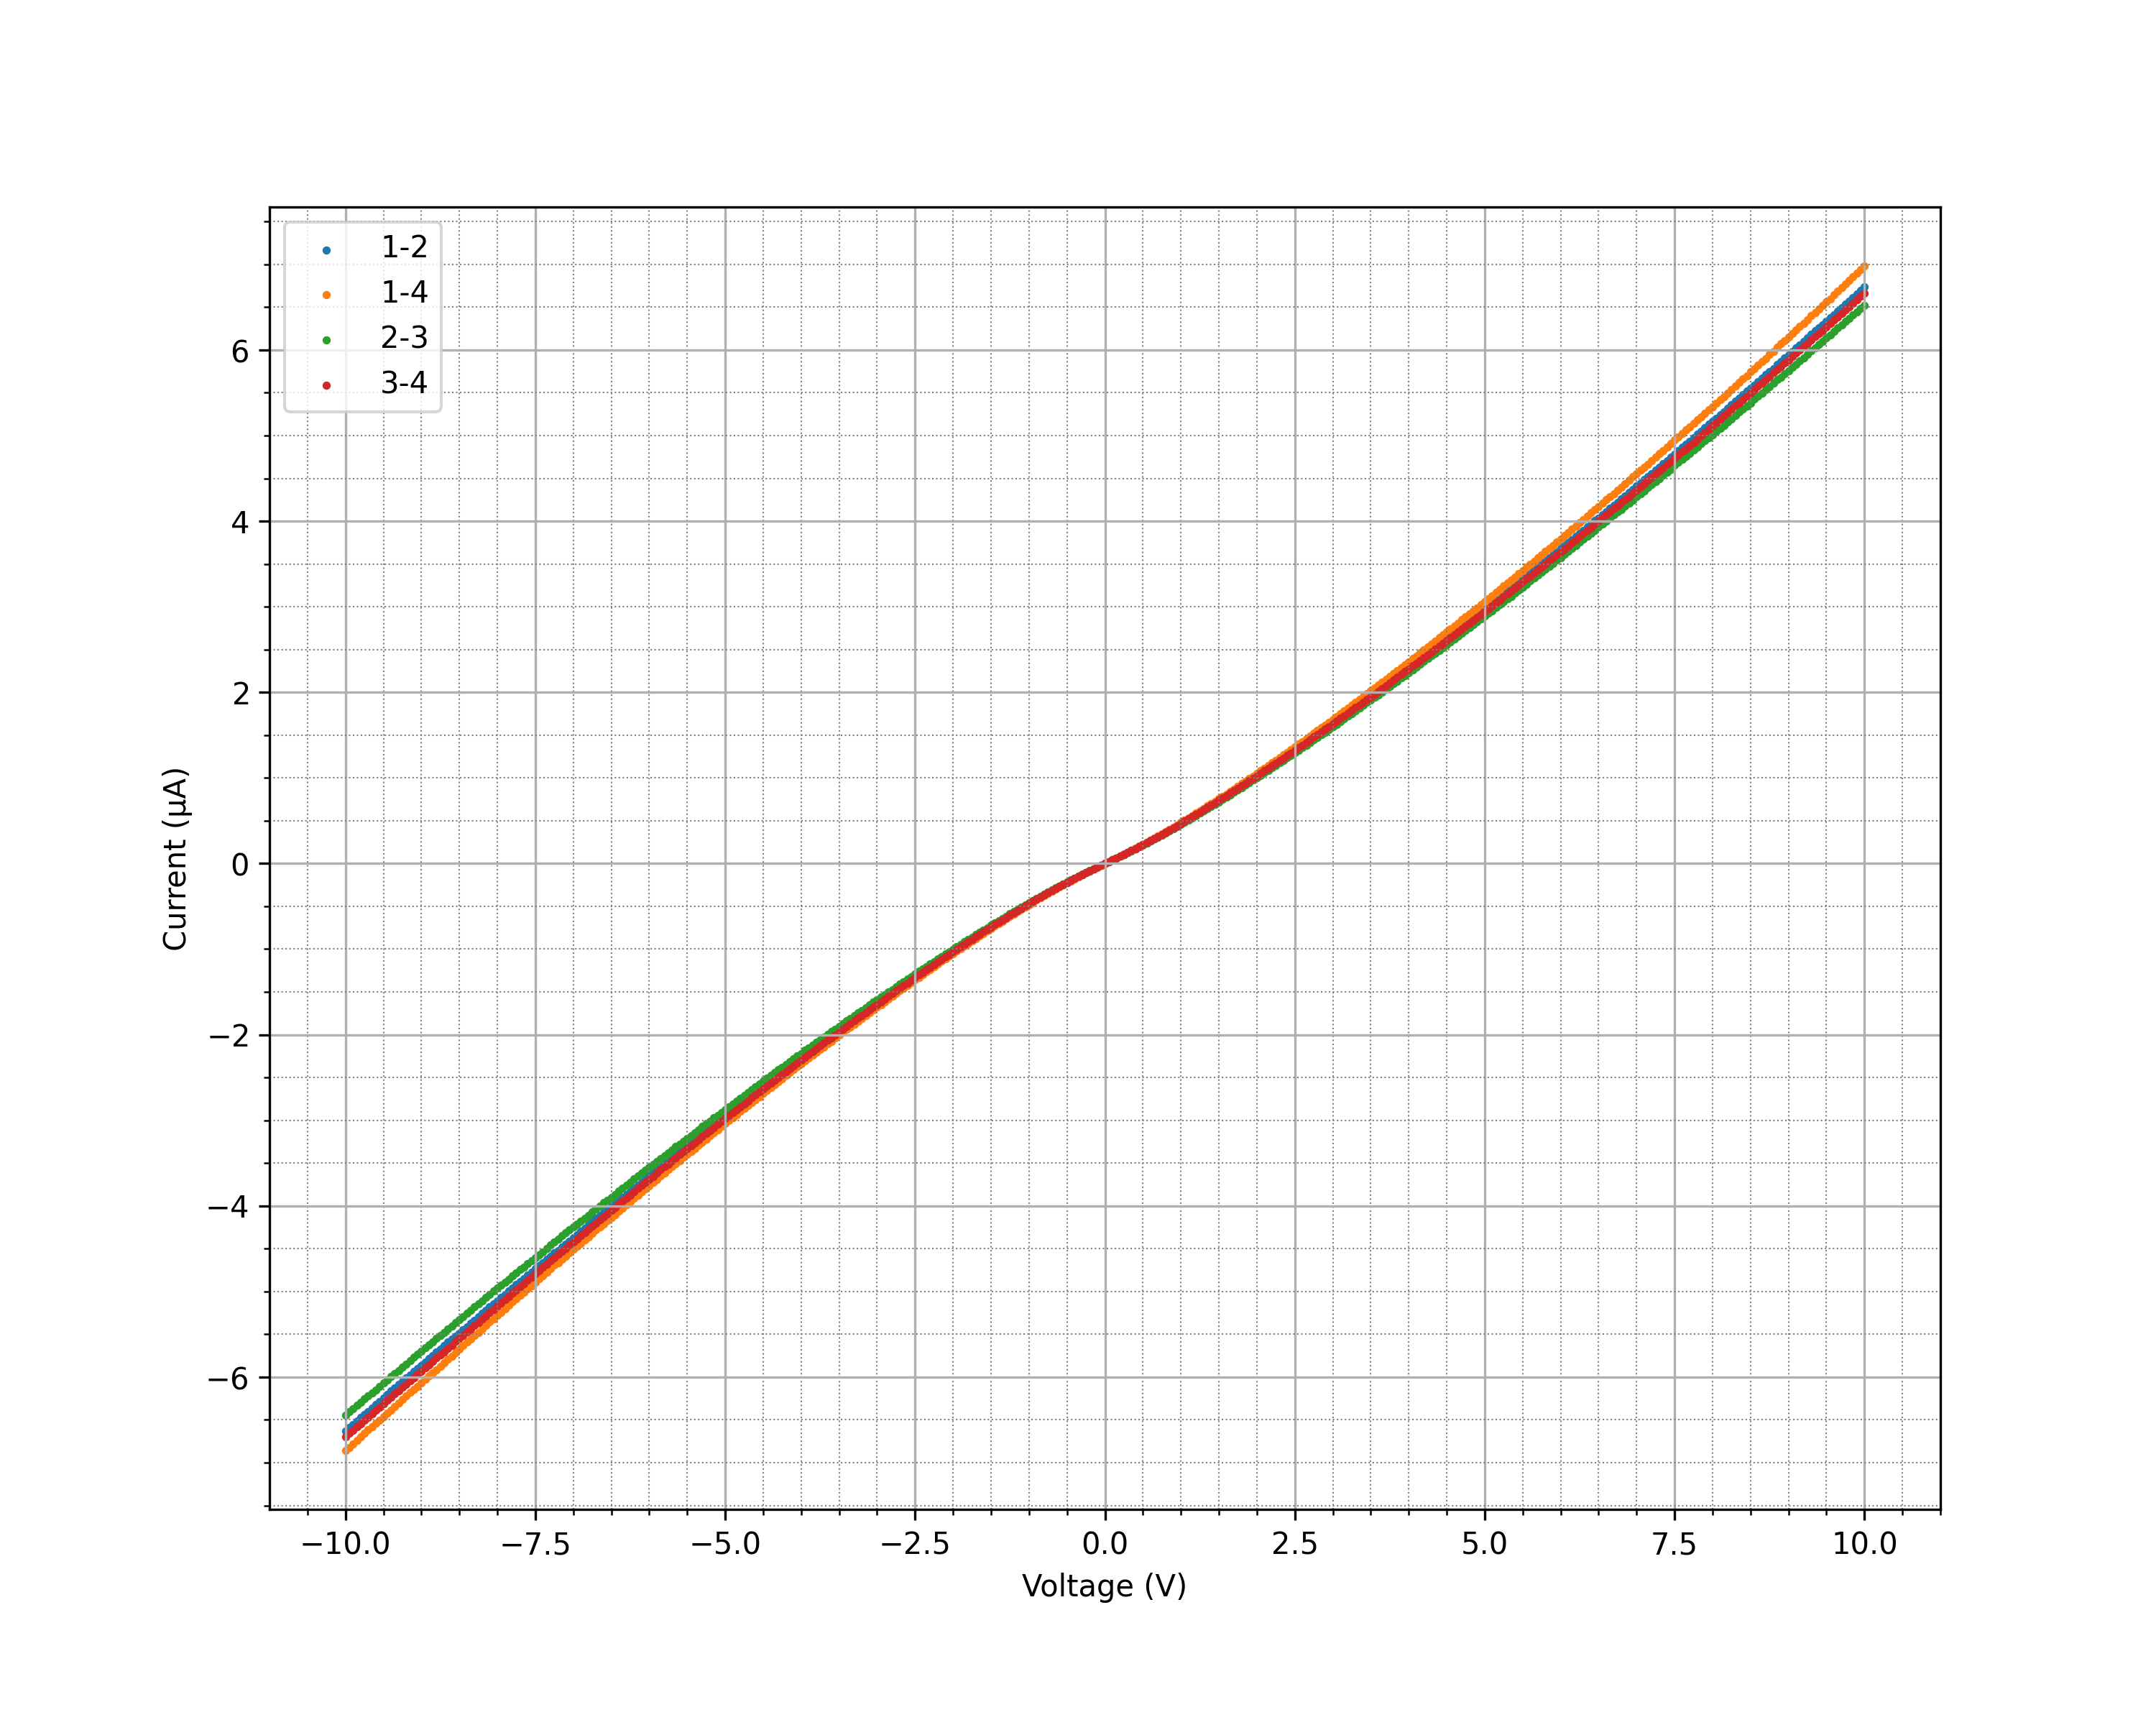
\includegraphics[width=\linewidth]{Chapter7/Figs/Raster/cross iv.png}
    \caption{The average IV characteristics across all four possible paths utilising the full wire test structure.}
    \label{fig:10v_big_bone}
\end{figure}

Figure \ref{fig:10v_big_bone} shows the overlay of all four differing sets of electrical measurements taken across the 14~\si{\micro\metre} wire via probes located on the 10~\si{\micro\metre} wires. It is difficult to see the dataset corresponding to the IV data between probes 1-2, as it very tightly follows the data for probes 3-4. Otherwise, there are only minor differences in the measured conductivities between these locations on the wire structure, and all four sets of measurements are in good agreement, despite the slight differences in wire lengths (1-2 $\sim295$~\si{\micro\metre}, 1-4/2-3 $\sim301$~\si{\micro\metre}, 3-4 $\sim305$~\si{\micro\metre}).

\begin{figure}[H]
    \centering
    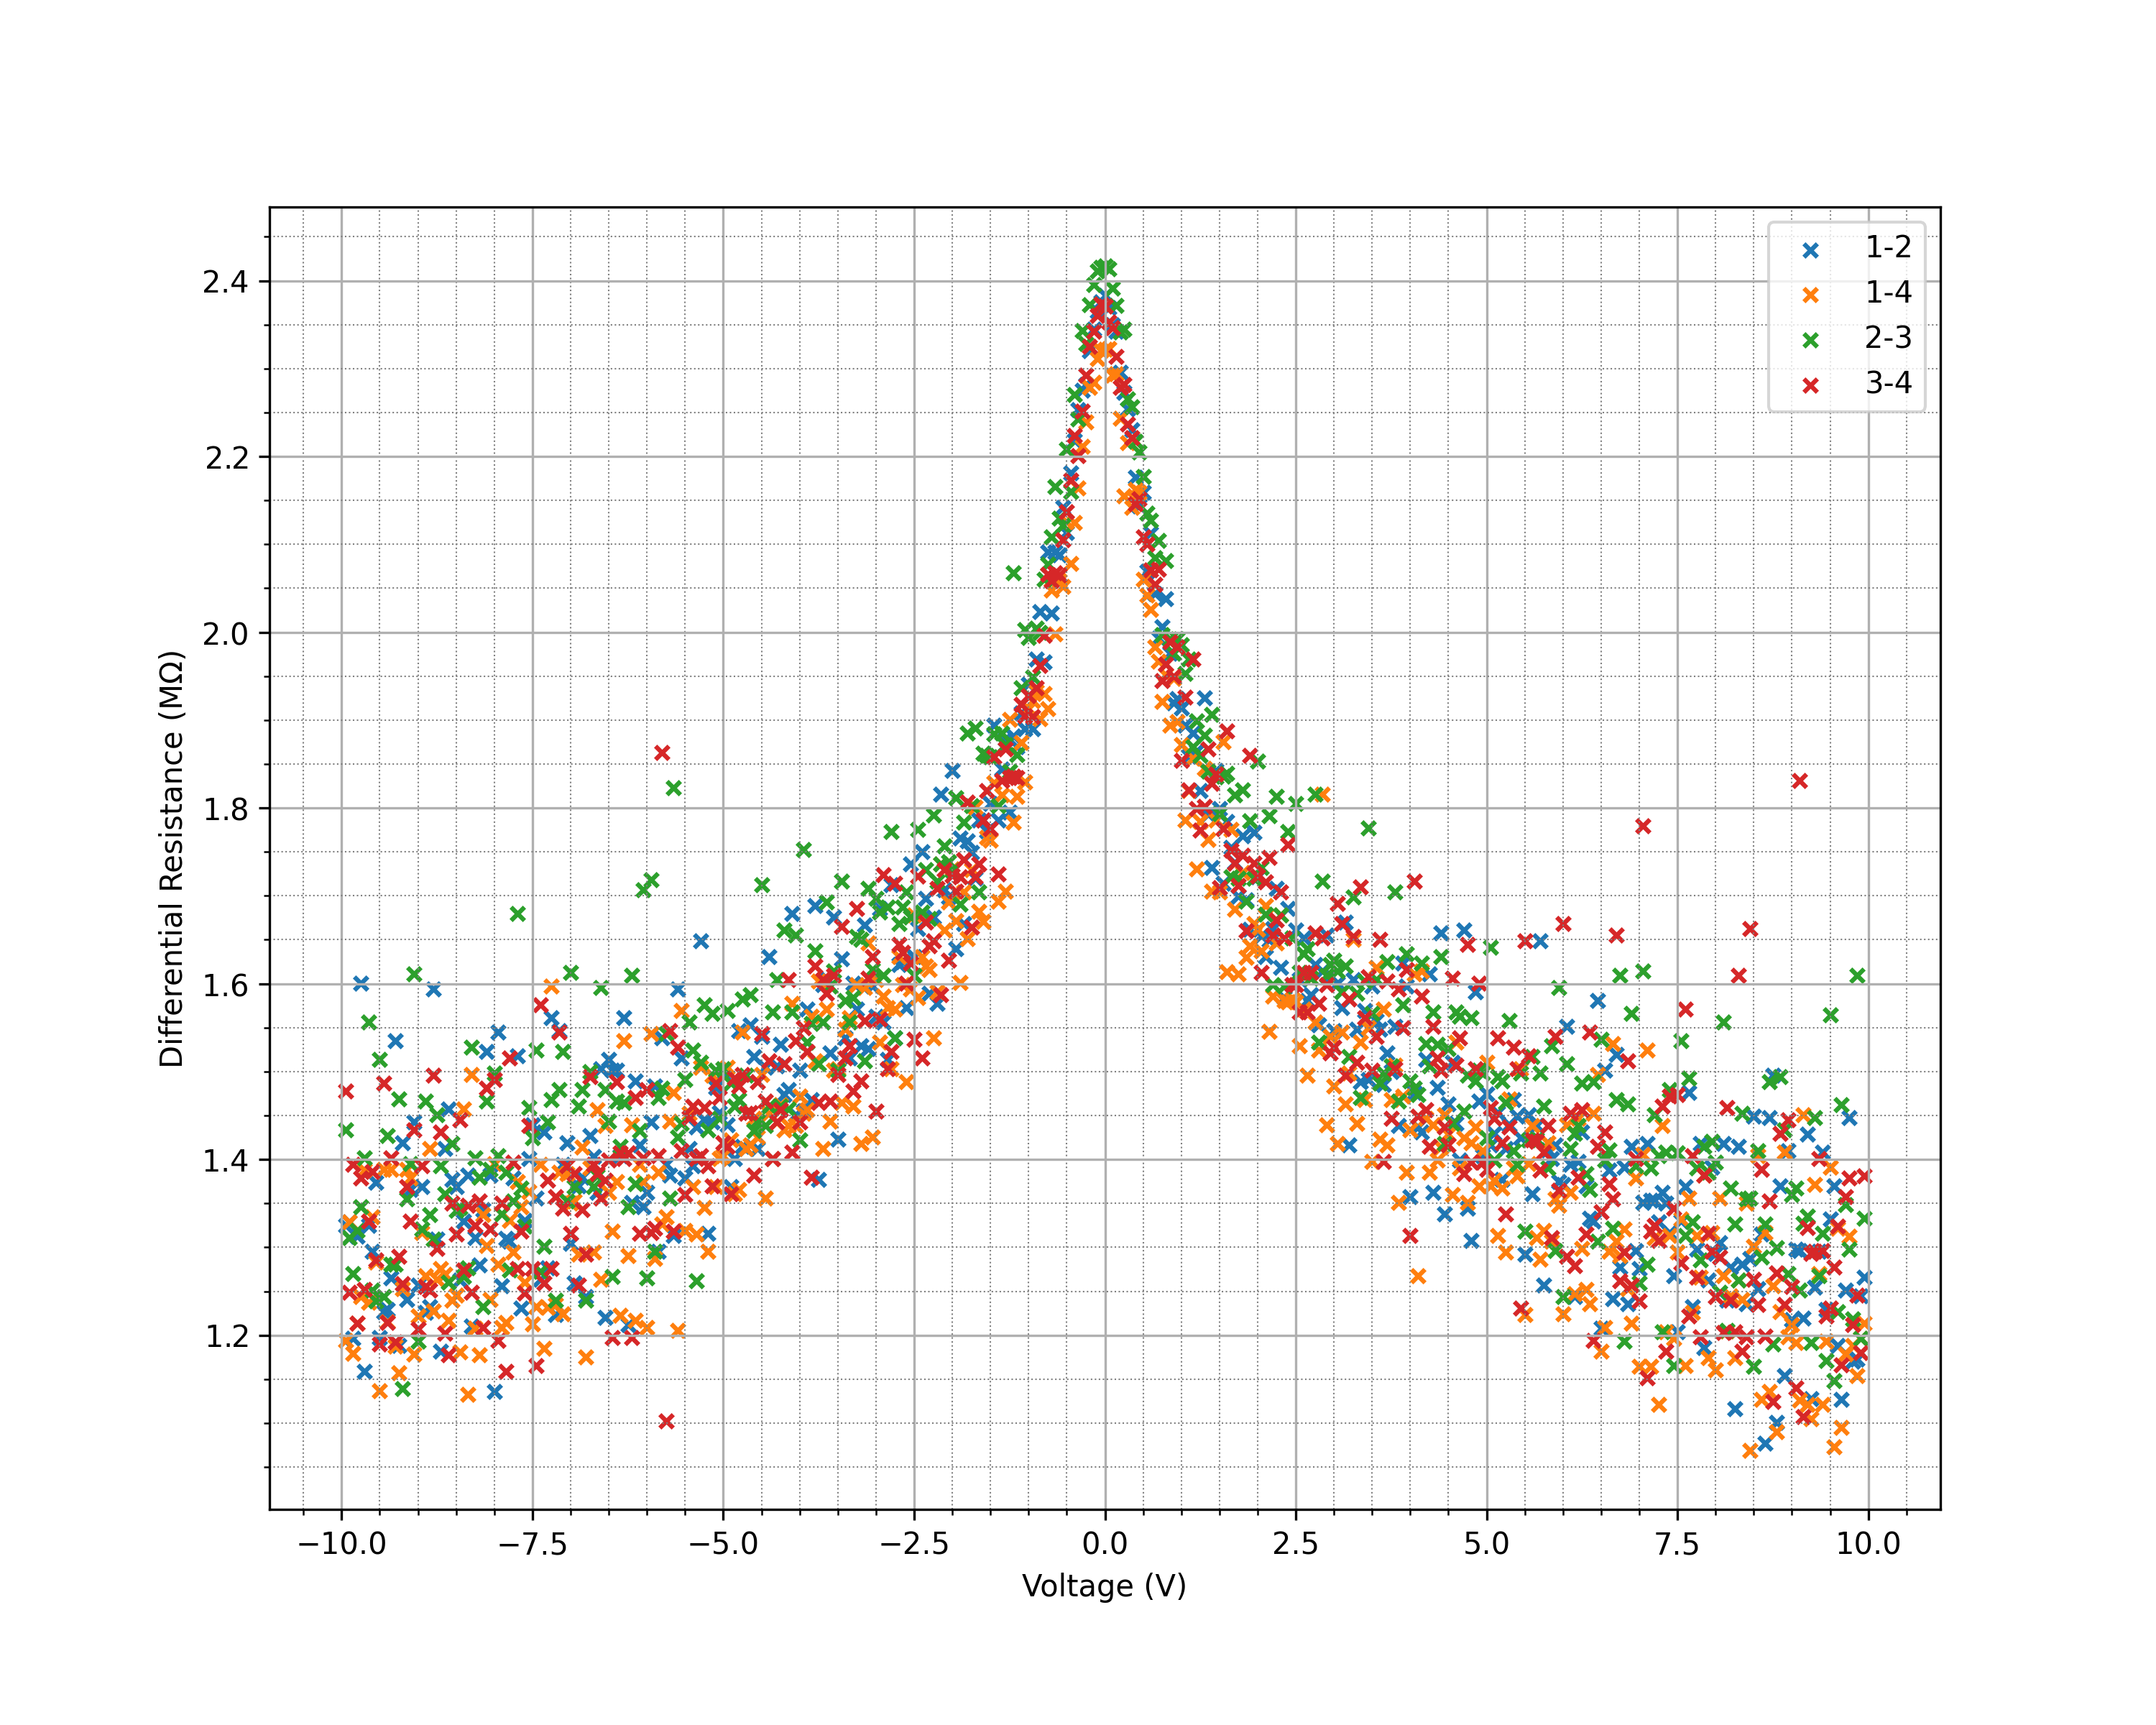
\includegraphics[width=\linewidth]{Chapter7/Figs/Raster/cross dr.png}
    \caption{The average differential resistance across all four possible paths utilising the full wire test structure.}
    \label{fig:10v_big_bone_dr}
\end{figure}

Figure \ref{fig:10v_big_bone_dr} shows an overlay of all four differential resistance plots across the test structure. Similar to the observations in figure \ref{fig:10v_big_bone}, the electrical characteristics are consistent across all paths. However, at higher voltages, a notable spread in differential resistance values is observed. This variability might be attributed to the differing number of data points per sweep, with 1000 data points typically collected in most sweeps, and a minimum of 400 in others. More consistent sampling across sweeps, and increasing the number of data points, is likely to enhance the precision and reduce the variability of the results. Each IV sweep was performed three times, spaced by a minimum of 10 seconds between each sweep to mitigate any effects of residual charge build-up, ensuring that the measurements reflect the true resistance of the wire without interference from transient electrical effects.

\begin{table}[ht]
\centering
\begin{tabular}{|c|c|c|c|c|}
\hline
Path & Resistance (M$\Omega$) & Resistivity ($\Omega$cm) & Conductivity (S/m) & Error (S/m) \\
\hline
1-2 & $1.58$ & $3.21$ & $31.1$ & $2.22$ \\
1-4 & $1.53$ & $3.05$ & $32.7$ & $2.34$ \\
3-2 & $1.63$ & $3.25$ & $30.8$ & $1.06$ \\
3-4 & $1.58$ & $3.11$ & $32.2$ & $1.09$ \\
\hline
A-B & $0.992$ & $4.24$ & $23.6$ & $1.44$ \\
1-3 & $0.0438$ & $0.156$ & $640$ & $45.7$ \\
2-4 & $0.0370$ & $0.132$ & $756$ & $54.0$ \\
\hline
\end{tabular}
\caption{Summary of electrical measurements at 10~\si{\volt} for different probe configurations.}
\label{table:electrical_measurements_10v_all}
\end{table}

In table \ref{table:electrical_measurements_10v_all}, the various electrical measurements across all four different "cross" configurations. Note that the calculation of resistivity and hence conductivity in this table uses an average wire width of 12~\si{\micro\metre} (in the first half), to provide an estimate for comparison with previous measurements across single wires. These measurements can be interpreted as three separate resistors in series, utilising wires that were characterised individually in the lower half of the table. All four electrical paths showed a reasonable similarity, with the potential error due to probe positioning potentially negating the slight differences observed. The lower half of the table provides the final measurements for each individual wire section, which highlights again the dominance of the resistance caused by the 14~\si{\micro\metre} wire.

\begin{figure}[H]
    \centering
    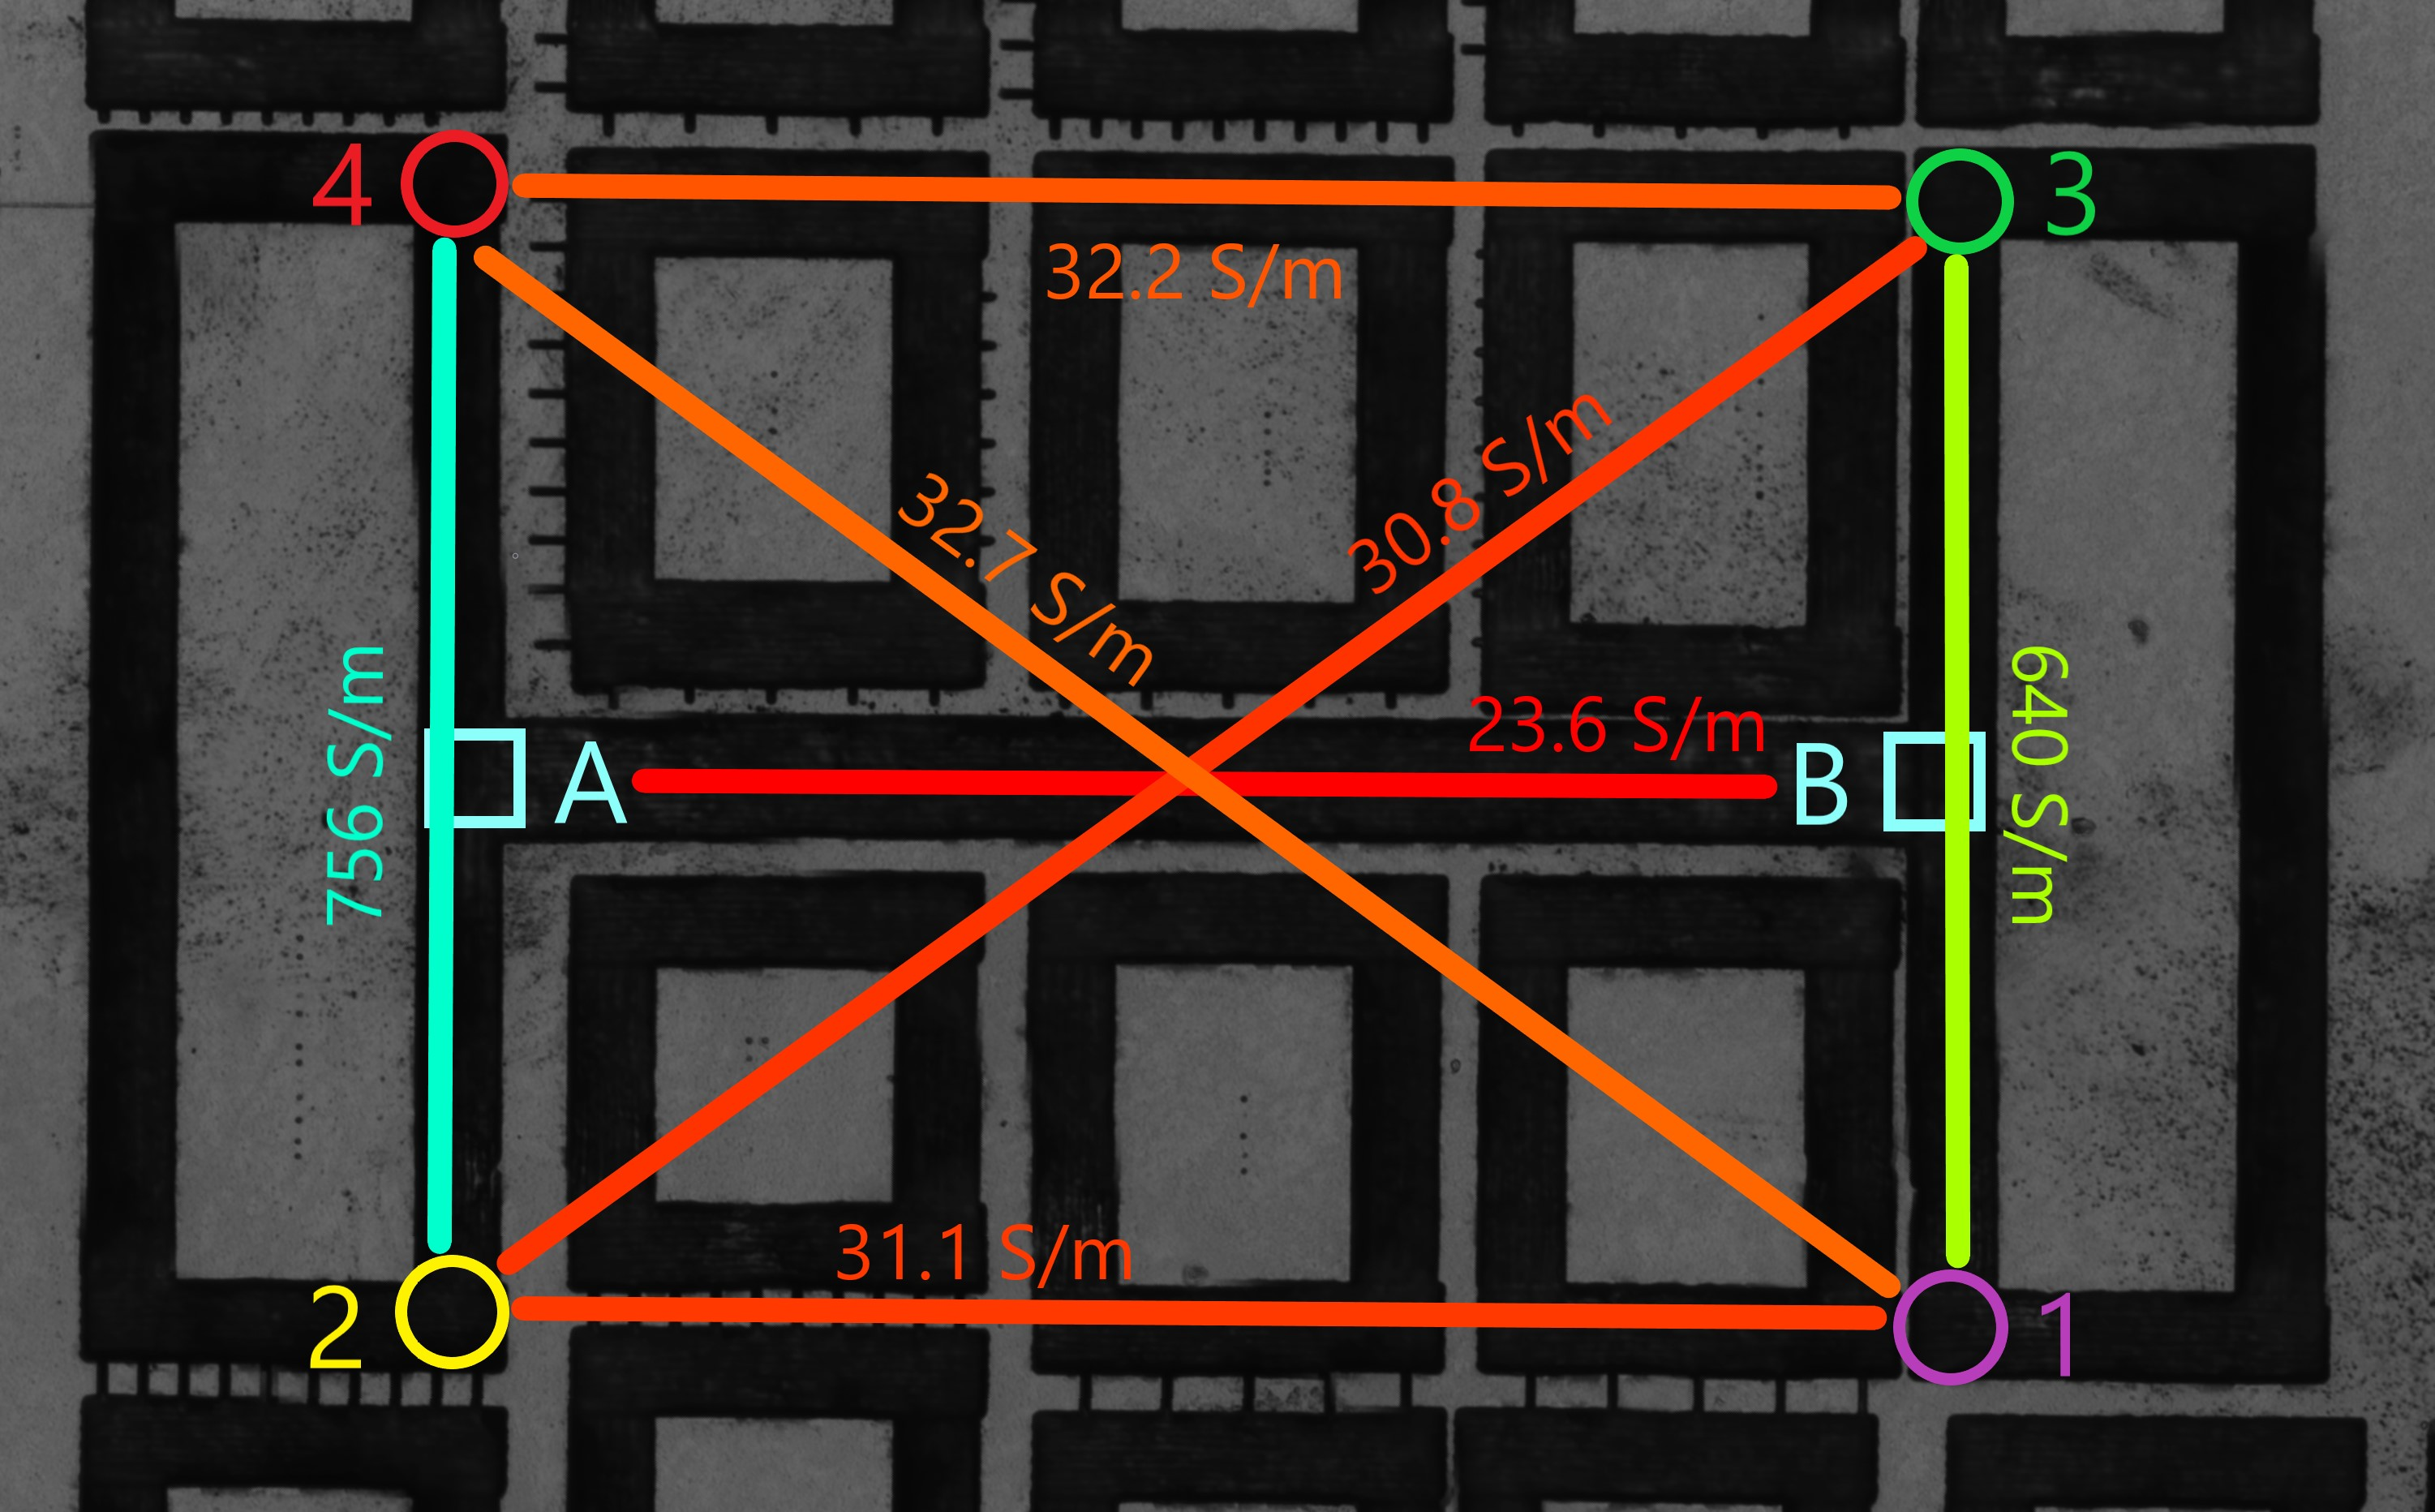
\includegraphics[width=\linewidth]{Chapter7/Figs/Raster/big_bone_esid_annotated_2.jpg}
    \caption{A simplified summary of the electrical characterisation of wire structures, as observed at 10~\si{\volt}.}
    \label{fig:big_bone_esid_2}
\end{figure}

Figure \ref{fig:big_bone_esid_2} provides a visual representation of the electrical measurements performed to determine the effectiveness of laser writing in creating ohmic wire structures. A colour spectrum is used with the simplified straight line connections to show the relative conductivities for the differing paths. The most noteworthy conclusion from these measurements was that the 10~\si{\micro\metre} wires were not merely ohmic, but were in fact significantly more ohmic than what was presumed to be the most electrically conductive structure in the design (the 14~\si{\micro\metre} wide wire). While there are some slight differences in the conductive paths that utilise both the cross bar and the thinner wires, the differences are not significant enough with the error analysis to conclude that any particular parts of the wires were more or less conductive. This is represented by the slight shift from red-orange that is present in the straight line connections used to represent these electrical paths. The only clear difference was between the two 10~\si{\micro\metre} wires, which showed an 18\% conductivity improvement in the leftmost wire between points 4-2, when compared to the rightmost wire between points 3-1.

\subsubsection{Comparison to Graphite}
\label{subsubsec:comparison_to_graphite}
With the measured conductivities following a number of assumptions regarding the geometric properties of the laser written wires, it is now a reasonable step to compare these values to what might be expected from ideal graphite wires. Then, it is possible to ask what the geometry of these graphite wires must be to match the measured resistances. It is inferred that the thickness of such a pure graphite wire must follow:
\begin{equation}
    t = \frac{L}{\sigma RW}
    \label{eq:thickness_conductivity}
\end{equation}

Using a low estimate of the basal plane conductivity for typical graphite ($\sim2\times10^{5}~\si{\siemens\per\metre}$ \cite{pierson1993}, and by comparing to the measured resistance for the highest calculated conductivity of $756$~\si{\siemens\per\metre} (path 2-4, as outlined in table \ref{table:electrical_measurements_10v_all}), the effective thickness of such an ideal wire is calculated to be $1.89$~\si{\nano\metre} in thickness. While the inter-atomic spacing between graphene sheets within graphite is a strong function of temperature and also depends upon the stacking sequence, typical inter-layer spacings are of the order of $0.355$~\si{\nano\metre} \cite{pierson1993}. Hence, a low estimate of basal plane conductivity for ideal graphite indicates an effective wire of only $\sim5$ layers of thickness.

If instead, conduction is considered perpendicular to the basal plane of $\sim300$~\si{\siemens\per\metre} \cite{pierson1993}, and again the highest calculated conductivity wire is used as a resistance reference point, the effective thickness of this wire is calculated to be $1.26$~\si{\micro\metre}. This is not too surprising, since the assumption of thickness $0.5$~\si{\micro\metre} was used in the calculation of conductivity $756$~\si{\siemens\per\metre} for this wire originally. It does however confirm that for the electrical characteristics as performed on the 10~\si{\micro\metre} wide wires, graphite-like conductivity over a wire thickness that is reasonable does appear to be observed. Indeed the conductivity is more than 2 times higher when it is assumed that the thickness is $0.5$~\si{\micro\metre}, which as discussed in section \ref{subsubsec:laser_writing_thickness} represents a fair estimate based on literature values. Much thicker than $1$~\si{\micro\metre} is unlikely, though further studies on laser graphitisation of diamond may help to elucidate the mechanisms determining the depth at which conductive material is generated, be that in the form of graphitic, diaphitic, or segregated areas of sp$^{2}$ bonding in a percolative network, as well as the interplay between these materials in conductors.

Finally, for the case of lower conductivity, such as that for the wire between points A-B, considering graphitic conduction perpendicular to the basal plane of $\sim300$\si{\siemens\per\metre} \cite{pierson1993}, the effective thickness for the measured resistance is $39.4$\si{\nano\metre}. It is certainly possible that the assumption of relatively uniform graphitised material may be significantly incorrect in this wire, with some narrow conductive paths leading to the observed resistance. However this is at least mildly odd, implying that despite the wire being significantly wider, the conductive path formed is substantially more inconsistent in thickness to the degree that the additional width is irrelevant. This is perhaps another indicator that the conductive material formed by this process cannot be simply regarded as "graphitic", despite the successful application of such a descriptor to the thinner wires. Instead, it must be considered that such conduction is due to electrical percolation and nanostructure assemblies as described by complex network theory \cite{mclachlan1990}, \cite{yao2020}. Broken type 2 diaphite is another likely contender in such poorly conducting material, with recent work examining the shift between ohmic and semiconducting material due to differing laser parameters highlighting the potential for such broken conductive paths to transition from ohmic type 1 diaphite wires to highly resistive type 2 diaphite wires \cite{salter2024}.

Usage of the low estimated conductivity for in-plane graphite leads to an effective thickness of $59$~\si{\pico\metre} when the values for path A-B are used again, around 7 times thinner than that of typical measured thicknesses of single graphene layers \cite{shearer2016}. This provides further confirmation that on the scale from a thin highly conductive layer of sp${2}$ bonded carbon, to very thick, poorly conducting amorphous carbon containing sp$^{2}$ bonding, it must necessarily be well away from the edge case of a single graphene layer providing the bulk of observed conductivity. It is impossible to rule out a "broken islands" structure of graphene conductivity, but this is again leading to a complex network theory or electrical percolation model. In which case, it is more likely that layers of graphene are not the cause of conductivity.

Regardless of the exact geometric and material model underlying the observed conductive paths, these conductive paths are sufficient to provide electrical wires embedded within the diamond surface. The contact between such wires and the phosphorous doped diamond surface layer may now be considered.

\subsection{LTLM Structure}

\begin{figure}[H]
    \centering
    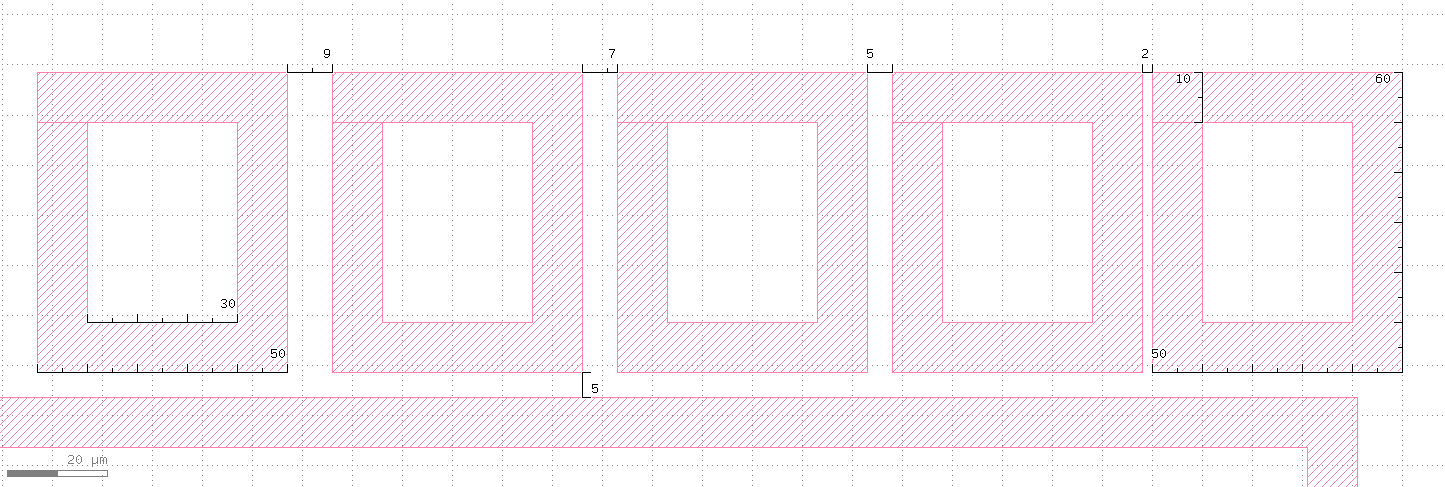
\includegraphics[width=\linewidth]{Chapter7/Figs/Raster/ltlm_design.png}
    \caption{The design of a LTLM structure for laser processing.}
    \label{fig:ltlm_design}
\end{figure}

As established in section \ref{subsubsec:comparison_to_graphite}, the electrical conductivity of the wires is sufficient to proceed with testing of diamond devices manufactured with these wires. In particular, one of the intended device structures is that of emitters, or emitter arrays. However before testing such devices, it is important to have a baseline of comparison, which in practical terms results in a simple LTLM structure, as that will provide a test of "emitter-less" devices. This has the additional benefit of providing a comparison to conventional Ti-based ohmic contacts, which rely on annealing to generate a TiC interlayer for the reduction of Schottky barrier height and the subsequent reduction in specific contact resistivity. Figure \ref{fig:ltlm_design} shows the designed structure of this LTLM-type setup. Four channel lengths between 2--9~\si{\micro\metre} are included, with simple rectangular wires providing the effective contacts. As shown in section \ref{subsec:afm_characterisation}, the channel width as measured via topological surveys shows some error in particular locations. It is important to examine these contacts prior to any LTLM analysis, due to the potential for significant deviation from the intended device structure.

\subsubsection{LTLM Microscopy}

\begin{figure}[H]
    \centering
    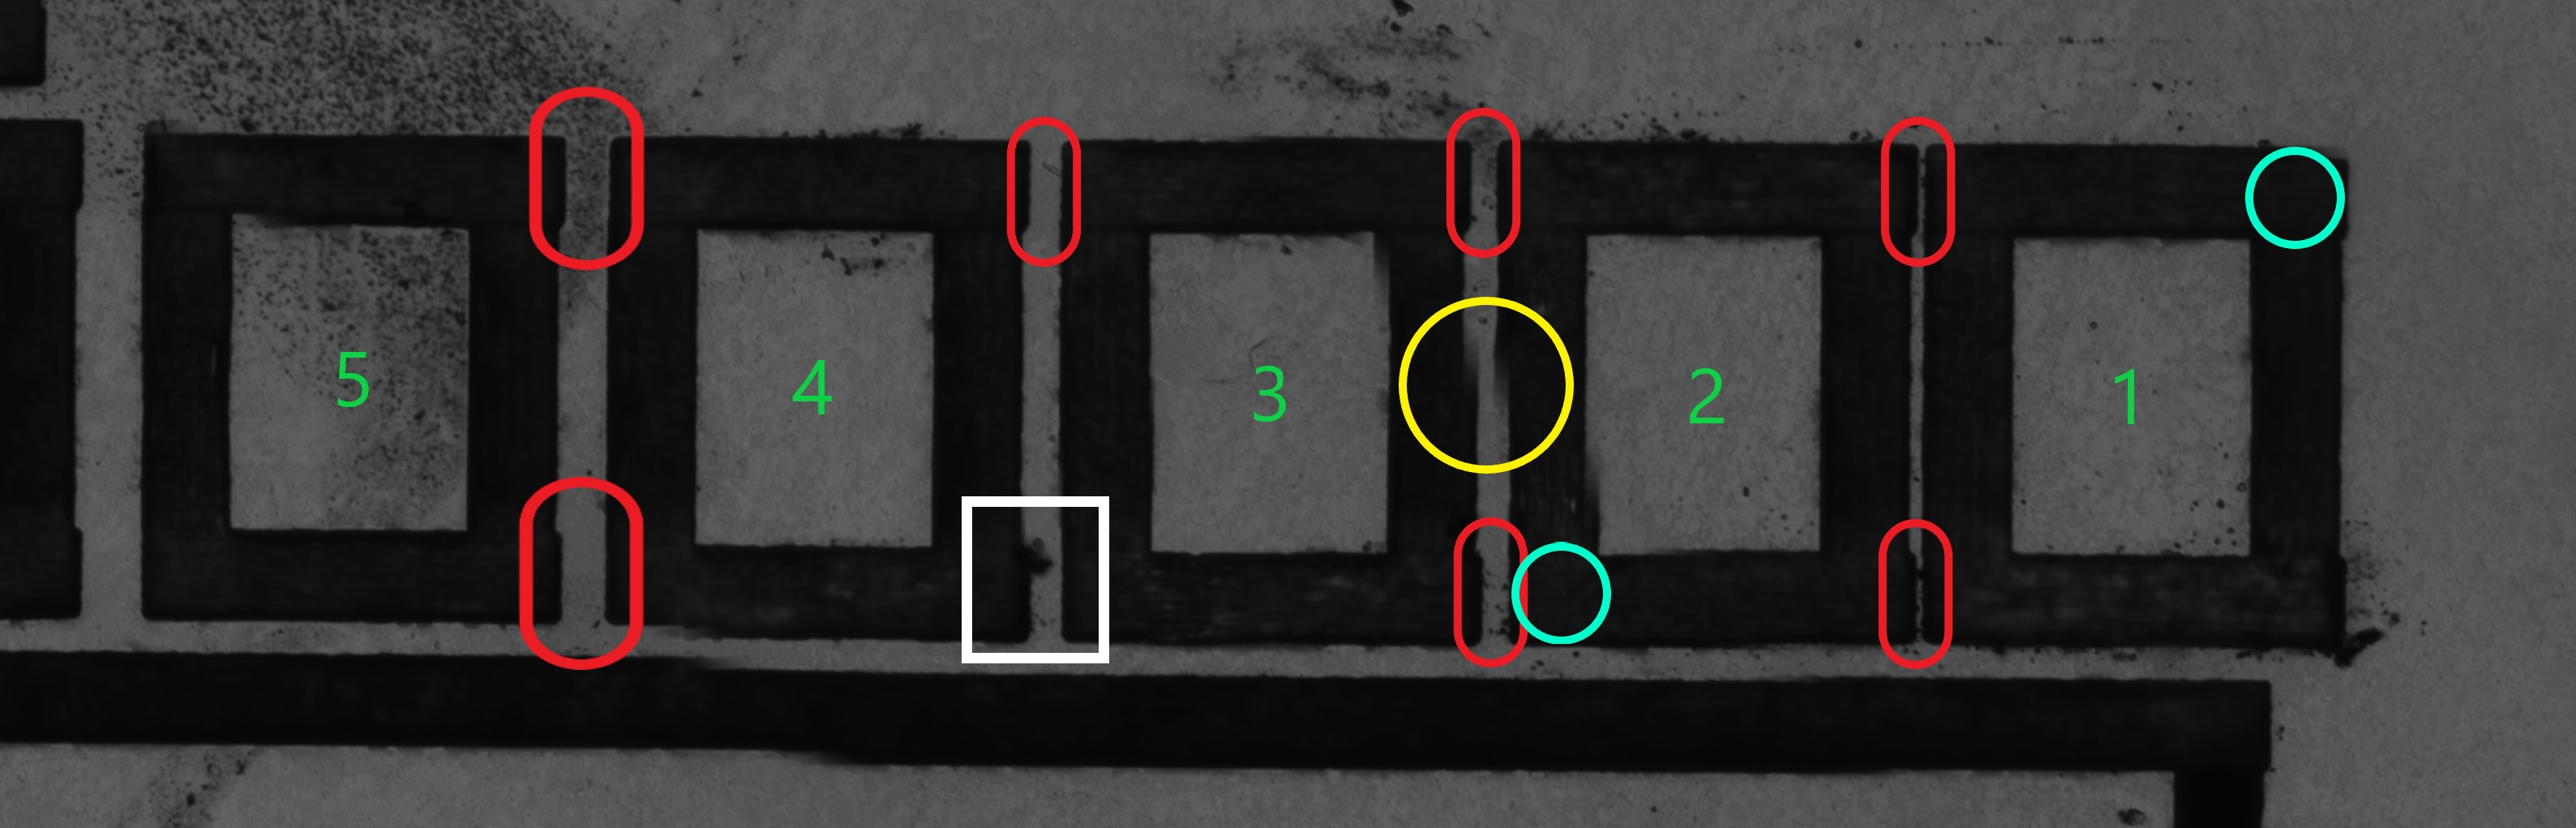
\includegraphics[width=\linewidth]{Chapter7/Figs/Raster/ltlm_esid_annotated4.jpg}
    \caption{The LTLM laser written structure as observed via confocal microscopy with a 488~\si{\nano\metre} light source. Annotated numbers indicate the contact label.}
    \label{fig:ltlm_esid}
\end{figure}

Figure \ref{fig:ltlm_esid} shows the laser processed device structure as seen via confocal microscopy, utilising a 488~\si{\nano\metre} back-light. The different electrical wires used to form effective contact regions are labelled 5--1 from left to right. Red capsules are used to highlight corners of the contacts where it appears that a slight overshoot relative to the vertical wires has occurred. In the case of the channel between contacts 2-1, this results in what appears to be a potential overlap at this scale between the contacts in laser written graphitic content. In the case of the other channels it simply produces a small region at the corners where visible narrowing occurs. The yellow circle indicates what appears to be a slight mismatch in the vertical wires at the edges of contact 3 and 2. On contact 3, the wire appears to fade away to transparent diamond moving upwards and out of this circle, while on contact 2 the wire at the edge of the contact appears to similarly fade into transparency moving downwards. The net result is a region in the centre of the circle in particular where the channel appears to have its narrowest point, and significantly wider regions before the corners. Finally a white square highlights what appears to be an amorphous blob on the bottom right corner of contact 4. It is unclear if this is due to the laser writing, or if it is contamination on the surface of the diamond. A region of small, soot-like contamination appears in various locations of this image, particularly near contact 5. It is possible that this is graphitic material due to ablation during the laser processing, which has not been removed in the subsequent solvent cleaning steps. Other possibilities, such as absorbance of the back-lighting within the substrate itself, may be considered via examination of other microscopy imaging utilising a top-down light source.

A final detail included in figure \ref{fig:ltlm_esid} is that of the cyan circles on contacts 2 and 1. These represent the two probe locations which were used for electrical characterisation across the 2~\si{\micro\metre} channel. Similar positions were used for the rest of the LTLM channels, with the right-most probe being located on the upper right corner of the contact structure and the left-most contact positioned on the lower left corner of the corresponding contact. This was done to ensure as much consistency as possible with the electrical measurements, as changing the relative positions of the probes on the contacts beween channels would change the resistance due to the 10~\si{\micro\metre} wire resistivity. As previously established, the 10~\si{\micro\metre} wires demonstrate the highest electrical conductivity, so the voltage drop across these wires should be minimal in comparison to the phosphorous doped diamond channel. However, this factor cannot be overlooked and is considered in the analysis of electrical measurements.

\begin{figure}[H]
    \centering
    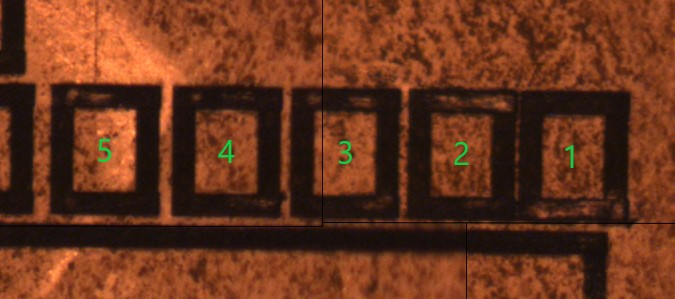
\includegraphics[width=\linewidth]{Chapter7/Figs/Raster/ltlm_afmm_annotated.jpg}
    \caption{The LTLM laser written structure as observed via optical microscopy with a white light source.}
    \label{fig:ltlm_afmm}
\end{figure}

Figure \ref{fig:ltlm_afmm} shows a tiled image of the LTLM structure, as seen with a standard optical microscope (air immersion). The resolution of this image is significantly lower than that of the back-lit microscopy shown in figure \ref{fig:ltlm_esid}, but it provides another visual comparison of the LTLM structure. In particular, the concentration of absorbent soot-like contamination near contact 5 is now visible as a reflective region on the surface of the sample, in contrast to the other areas which are not reflective.

\begin{figure}[H]
    \centering
    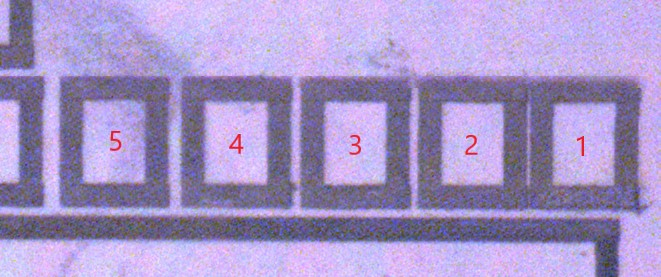
\includegraphics[width=\linewidth]{Chapter7/Figs/Raster/ltlm_afmm_dark_annotated.jpg}
    \caption{The LTLM laser written structure as observed via optical microscopy with a back-lit white light source.}
    \label{fig:ltlm_afmm_dark}
\end{figure}

Figure \ref{fig:ltlm_afmm_dark} provides a white back-lit image of the LTLM devices, using the same optical microscope as for the top-down white light source imaging in figure \ref{fig:ltlm_afmm}. Similar to that of the 488~\si{\nano\metre} back-lit confocal microscopy of figure \ref{fig:ltlm_esid}, the soot-like contamination around contact 5 is seen to absorb a fraction of the white light source. It is notable that in contrast to the complete absorption of 488~\si{\nano\metre} light, this region does appear to have some transparency in the visible light range. However, given the significant disparity in optical resolution with this image, it is still possible that these particles are strongly absorbing the full visible light range. Regardless, this provides further comparative optical imaging for a qualitative examination of the device structures.

\begin{figure}[H]
    \centering
    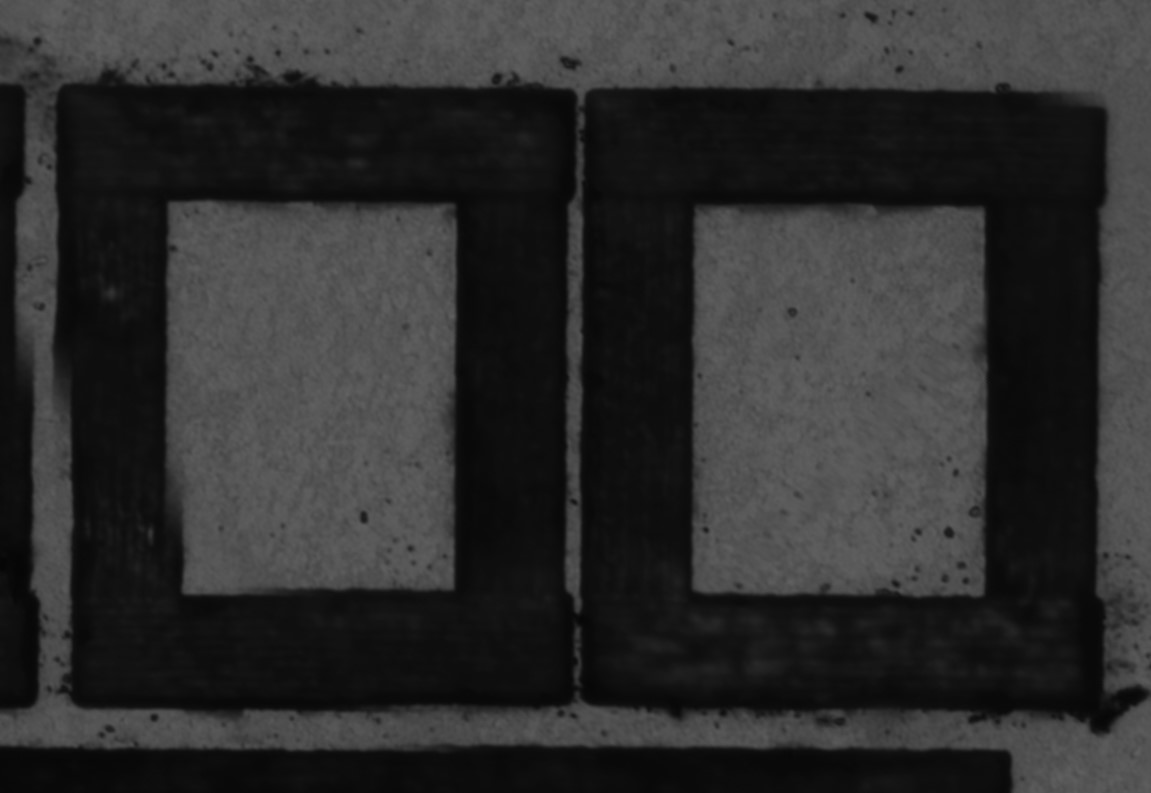
\includegraphics[width=\linewidth]{Chapter7/Figs/Raster/21_esid.jpg}
    \caption{Contacts 2-1 of the LTLM structure, more closely examined via 488~\si{\nano\metre} confocal microscopy.}
    \label{fig:21_esid}
\end{figure}

Figure \ref{fig:21_esid} provides a view of contacts 2-1, as viewed via 488~\si{\nano\metre} confocal microscopy. At this scale the limit due to diffraction is starting to become evident, since the estimated limit of spatial resolution for the oil-immersion confocal microscope used is 200~\si{\nano\metre} with the 488~\si{\nano\metre} laser used.

\begin{figure}[H]
    \centering
    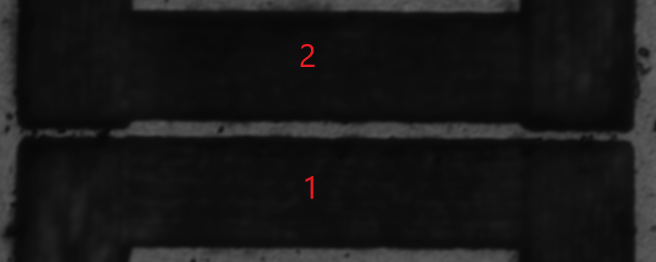
\includegraphics[width=\linewidth]{Chapter7/Figs/Raster/21 channel limit esid.png}
    \caption{Contacts 2-1 of the LTLM structure, at the optical limit via 488~\si{\nano\metre} confocal microscopy.}
    \label{fig:21_esid}
\end{figure}

\begin{figure}[H]
    \centering
    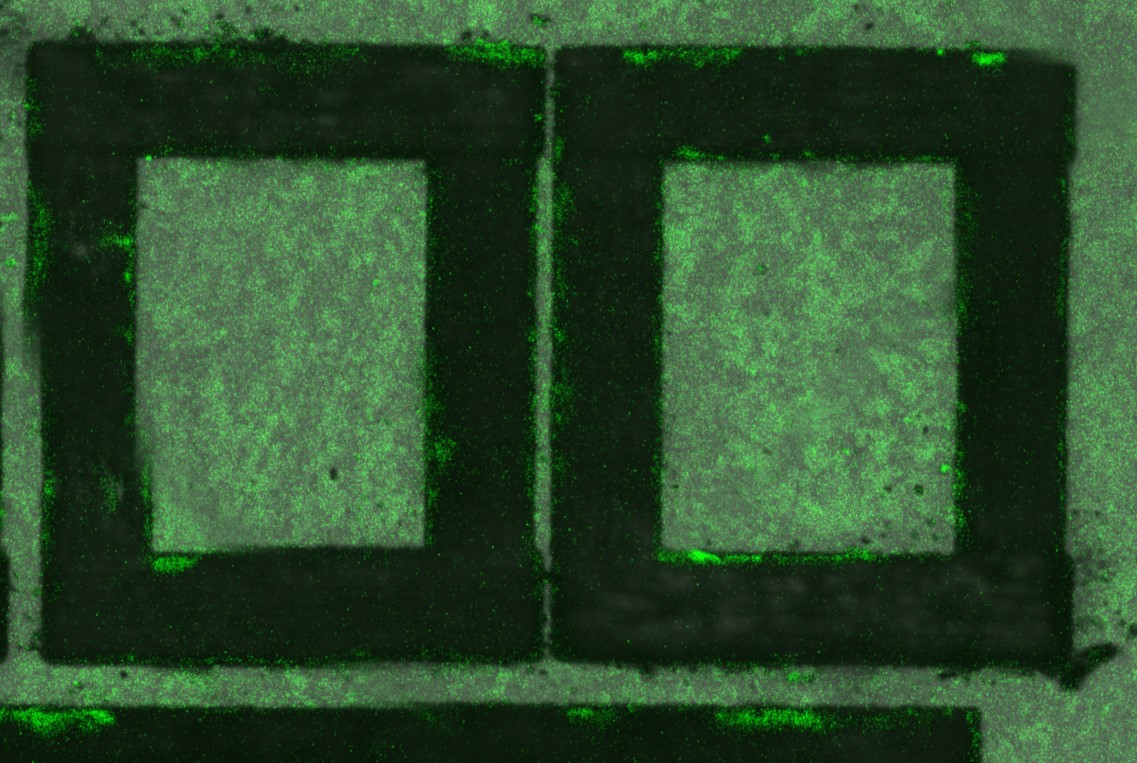
\includegraphics[width=\linewidth]{Chapter7/Figs/Raster/21_fl_esid.jpg}
    \caption{Contacts 2-1 of the LTLM structure, more closely examined via 488~\si{\nano\metre} confocal microscopy with 408~\si{\nano\metre} excited fluorescence.}
    \label{fig:21_fl_esid}
\end{figure}

In figure \ref{fig:21_fl_esid}, the fluorescence due to an excitation laser of 408~\si{\nano\metre} is overlaid onto the 488~\si{\nano\metre} confocal microscope imaging. While the source of any fluorescence is speculative, this provides another view of the laser written LTLM electrical contacts.

One noteworthy conclusion that is drawn from these high spatial resolution optical images of the contacts is that the slight overshoot observed at the corners of each contact appears to be touching at the bottom of the channel between contacts 2-1. At minimum, the spatial resolution of 200~\si{\nano\metre} is insufficient to resolve a clear spacing between the contacts in this region. As has been previously discussed in this chapter, the exact composition of laser processed wires and the resulting electrical characteristics could vary quite widely. While there is a visual "short" between the two contacts, if the dark material seen in this region is highly resistive, then the effective channel width may well still approach that of the designed 2~\si{\micro\metre}. While electrical characteristics indicating an intact semiconducting channel will help to disprove the existence of any electrical short, it is important to consider that the material connecting these two contacts may still be a semiconducting allotrope of carbon, but it may no longer be that of highly phosphorous doped diamond. This may distort the results if it is less resistive than that of the diamond channel, but still appear as though it is a semiconducting channel.

\begin{figure}[H]
    \centering
    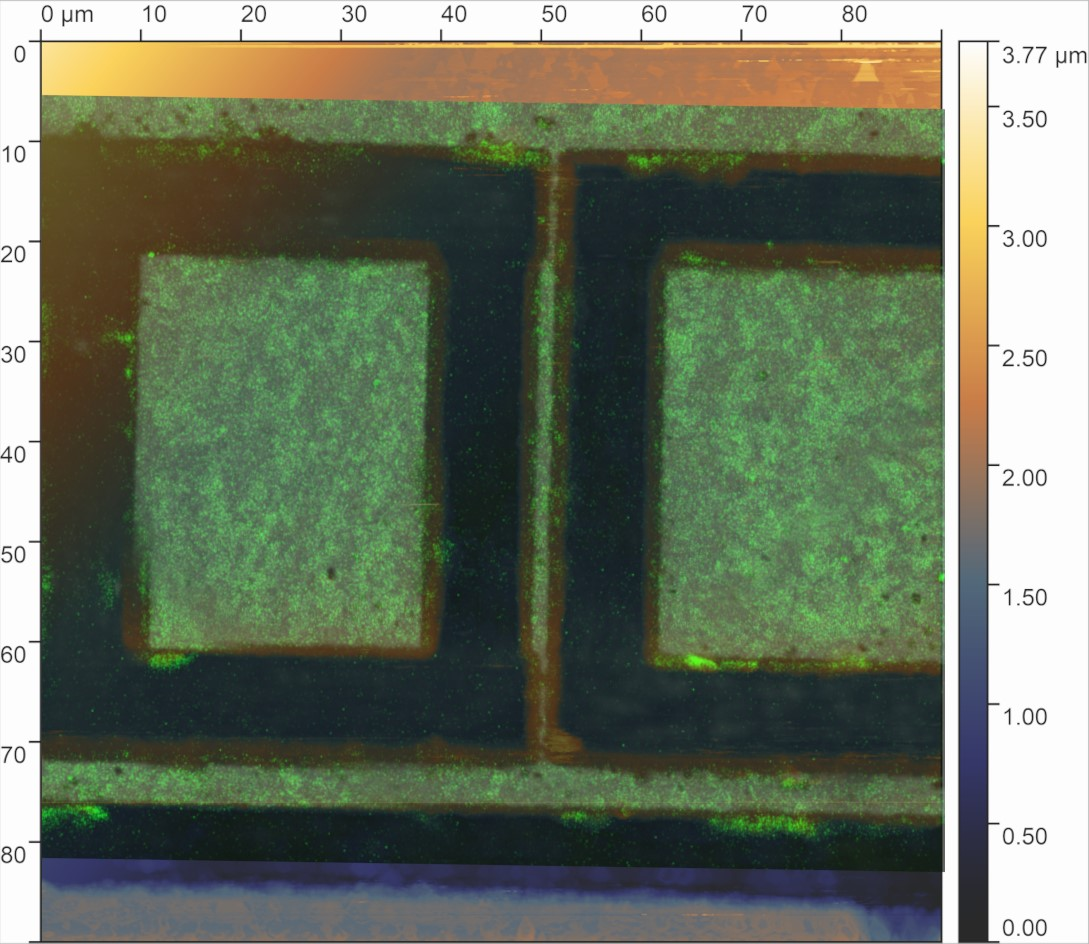
\includegraphics[width=\linewidth]{Chapter7/Figs/Raster/21_comparison.jpg}
    \caption{Contacts 2-1 of the LTLM structure, viewed as a combination of AFM, optical microscopy and fluorescence.}
    \label{fig:21_comparison}
\end{figure}

In figure \ref{fig:21_comparison}, an overlay of the oil-immersion fluorescent microscopy is fitted to the AFM characterisation taken for these two LTLM contacts. The fluorescent microscope imaging has had the transparency adjusted such that the deep blue used for the height associated with the bottom of the trenches is visible enough to observe the topological map. Note that while the visual inspection of these contacts reveals a link between the laser written wires in the lower portion of the channel, the topology reveals a clear lack of ablation in this region. This may have implications for the relative concentration of graphitic material present in the channel, as a lack of ablation will correlate with lower laser power or fluence \cite{Holly1998}, \cite{kononenko2005}. While the optically transparent diamond has been altered, a speculative conclusion may be that this material is unlikely to be highly graphitic, and hence much more resistive or at least semiconducting in nature. For the AFM topology only please see figure \ref{fig:afm_21_big}.

\subsubsection{2 Micron Channel IV Characteristics and LTLM Assumptions}
\label{subsubsec:2um channel iv characteristics and ltlm assumptions}
\begin{figure}[H]
    \centering
    \includegraphics[width=\linewidth]{Chapter7/Figs/Raster/21/21 Graphitised linear IV - Data within ±20.0V_IV_plot.png }
    \caption{A linear plot of the averaged IV characteristics across contacts 2-1. Error bars corresponding to a systematic error of 5\% are plotted.}
    \label{fig:21_linear_iv}
\end{figure}

Figure \ref{fig:21_linear_iv} shows the results of several trials of IV measurements across the channel between contacts 2-1. Several qualitative remarks can be made about the relationship displayed here, particularly in contrast to the previous experiments performed by the candidate using metal contacts and a LTLM structure in chapter \ref{ch:electrical_experiments}. Error bars of 5\% are included to account for the spread of data points observed between repeat attempts, and are hence a high estimate of systematic error based on the results themselves.

\begin{figure}[H]
    \centering
    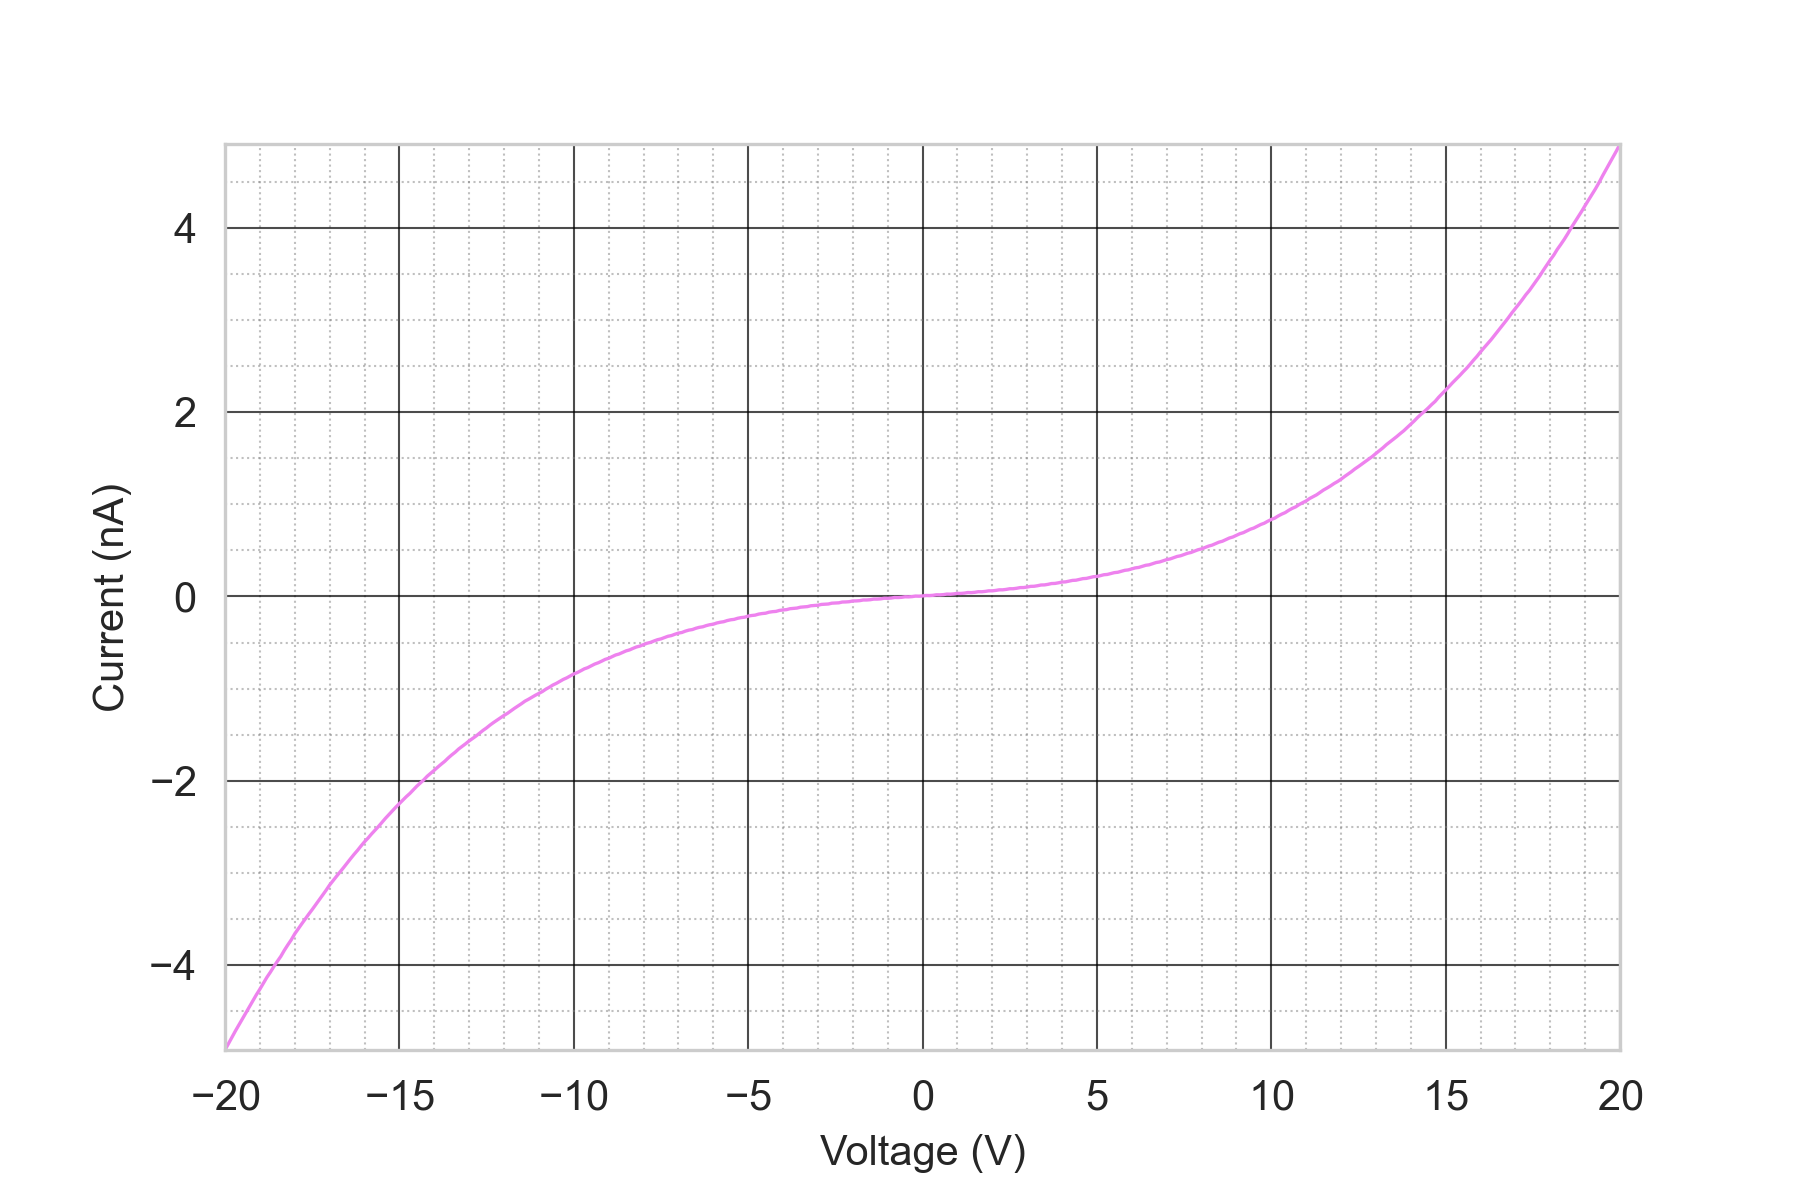
\includegraphics[width=0.8\linewidth]{Chapter7/Figs/Raster/20V IV characteristics at 21 C.png}
    \caption{A linear plot of the measured room temperature IV characteristics across the 2.8~\si{\micro\metre} LTLM channel for sample D (annealed Ti/Pt/Au contacts).}
    \label{fig:d_20v_linear}
\end{figure}

Figure \ref{fig:d_20v_linear} provides a visual reference to sample D, which also used a LTLM device structure for IV characterisation. The phosphorous doped diamond film on sample D was thinner than sample G's, at $\sim$0.3~\si{\micro\metre} against the laser processed $\sim$1.2~\si{\micro\metre} layer. If the only significant factor at play was the thickness of said phosphorous doped layer, with the resistivity remaining the same, then it would be expected that the measured resistance is a factor of 4 lower in the thicker sample. Given that at a bias of 20~\si{\volt}, across a 2.8\si{\micro\metre} channel, sample D had a measured current of $\sim$5~\si{\nano\ampere} and sample G with similar conditions and a $\sim$2~\si{\micro\metre} channel had a measured current of $\sim$93~\si{\milli\ampere}, there is an obvious $10^{7}$ magnitude shift in resistance which must be accounted for. There is also a clear change in behaviour from that of a single Schottky barrier, to what might represent a double Schottky barrier. As noted in the microscopy of channel 2-1, the observed channel width may differ from the designed $2$~\si{\micro\metre}. However even if the effective channel length is closer to $0.5$~\si{\micro\metre} alongside the known difference in thickness, this presents a geometrical factor of 16 in the observed resistance. Naturally, it is also possible to consider the resistivity as measured via CTLM, which presented a value of $\sim15$~\si{\ohm\centi\metre} with constant current condition of 1~\si{\micro\ampere}. The direct comparative work of Matsumoto et al. \cite{matsumoto2013} gives a value of $\sim9\times10^{-3}$~\si{\ohm\centi\metre} at a constant current condition of 50~\si{\micro\ampere} for similarly doped material. This methodology hence indicated that the majority of the measured resistance was due to the metal contacts, agreeing by and large with the two LTLM samples (C and D). The exact measurements of specific contact resistivity and resistivity do raise questions regarding the quality of metal contacts and homogeneity of highly phosphorous doped diamond, but the key concurring factor with metal contacts on phosphorous doped diamond is that of the extremely high specific contact resistivity that has been observed over a range of annealing conditions. Hence, while the geometry of this laser processed LTLM is largely intended to provide a benchmark for the emitter arrays, a key takeaway from the comparison of IV characteristics represented by figures \ref{fig:21_linear_iv} and \ref{fig:d_20v_linear} may be that the laser written structure is now providing a significantly reduced specific contact resistivity, even prior to the application of LTLM methodology. There are numerous assumptions that must be made to apply the quantitative methodology of the LTLM method in this case, with the channel length, local resistivity, contact wire conductivity and laser written geometry all factors that may affect the results. Be that as it may, the application of LTLM methodology was employed to provide a more direct comparison between metal contacts and laser written contacts.

\subsubsection{LTLM}
\begin{figure}[H]
    \centering
    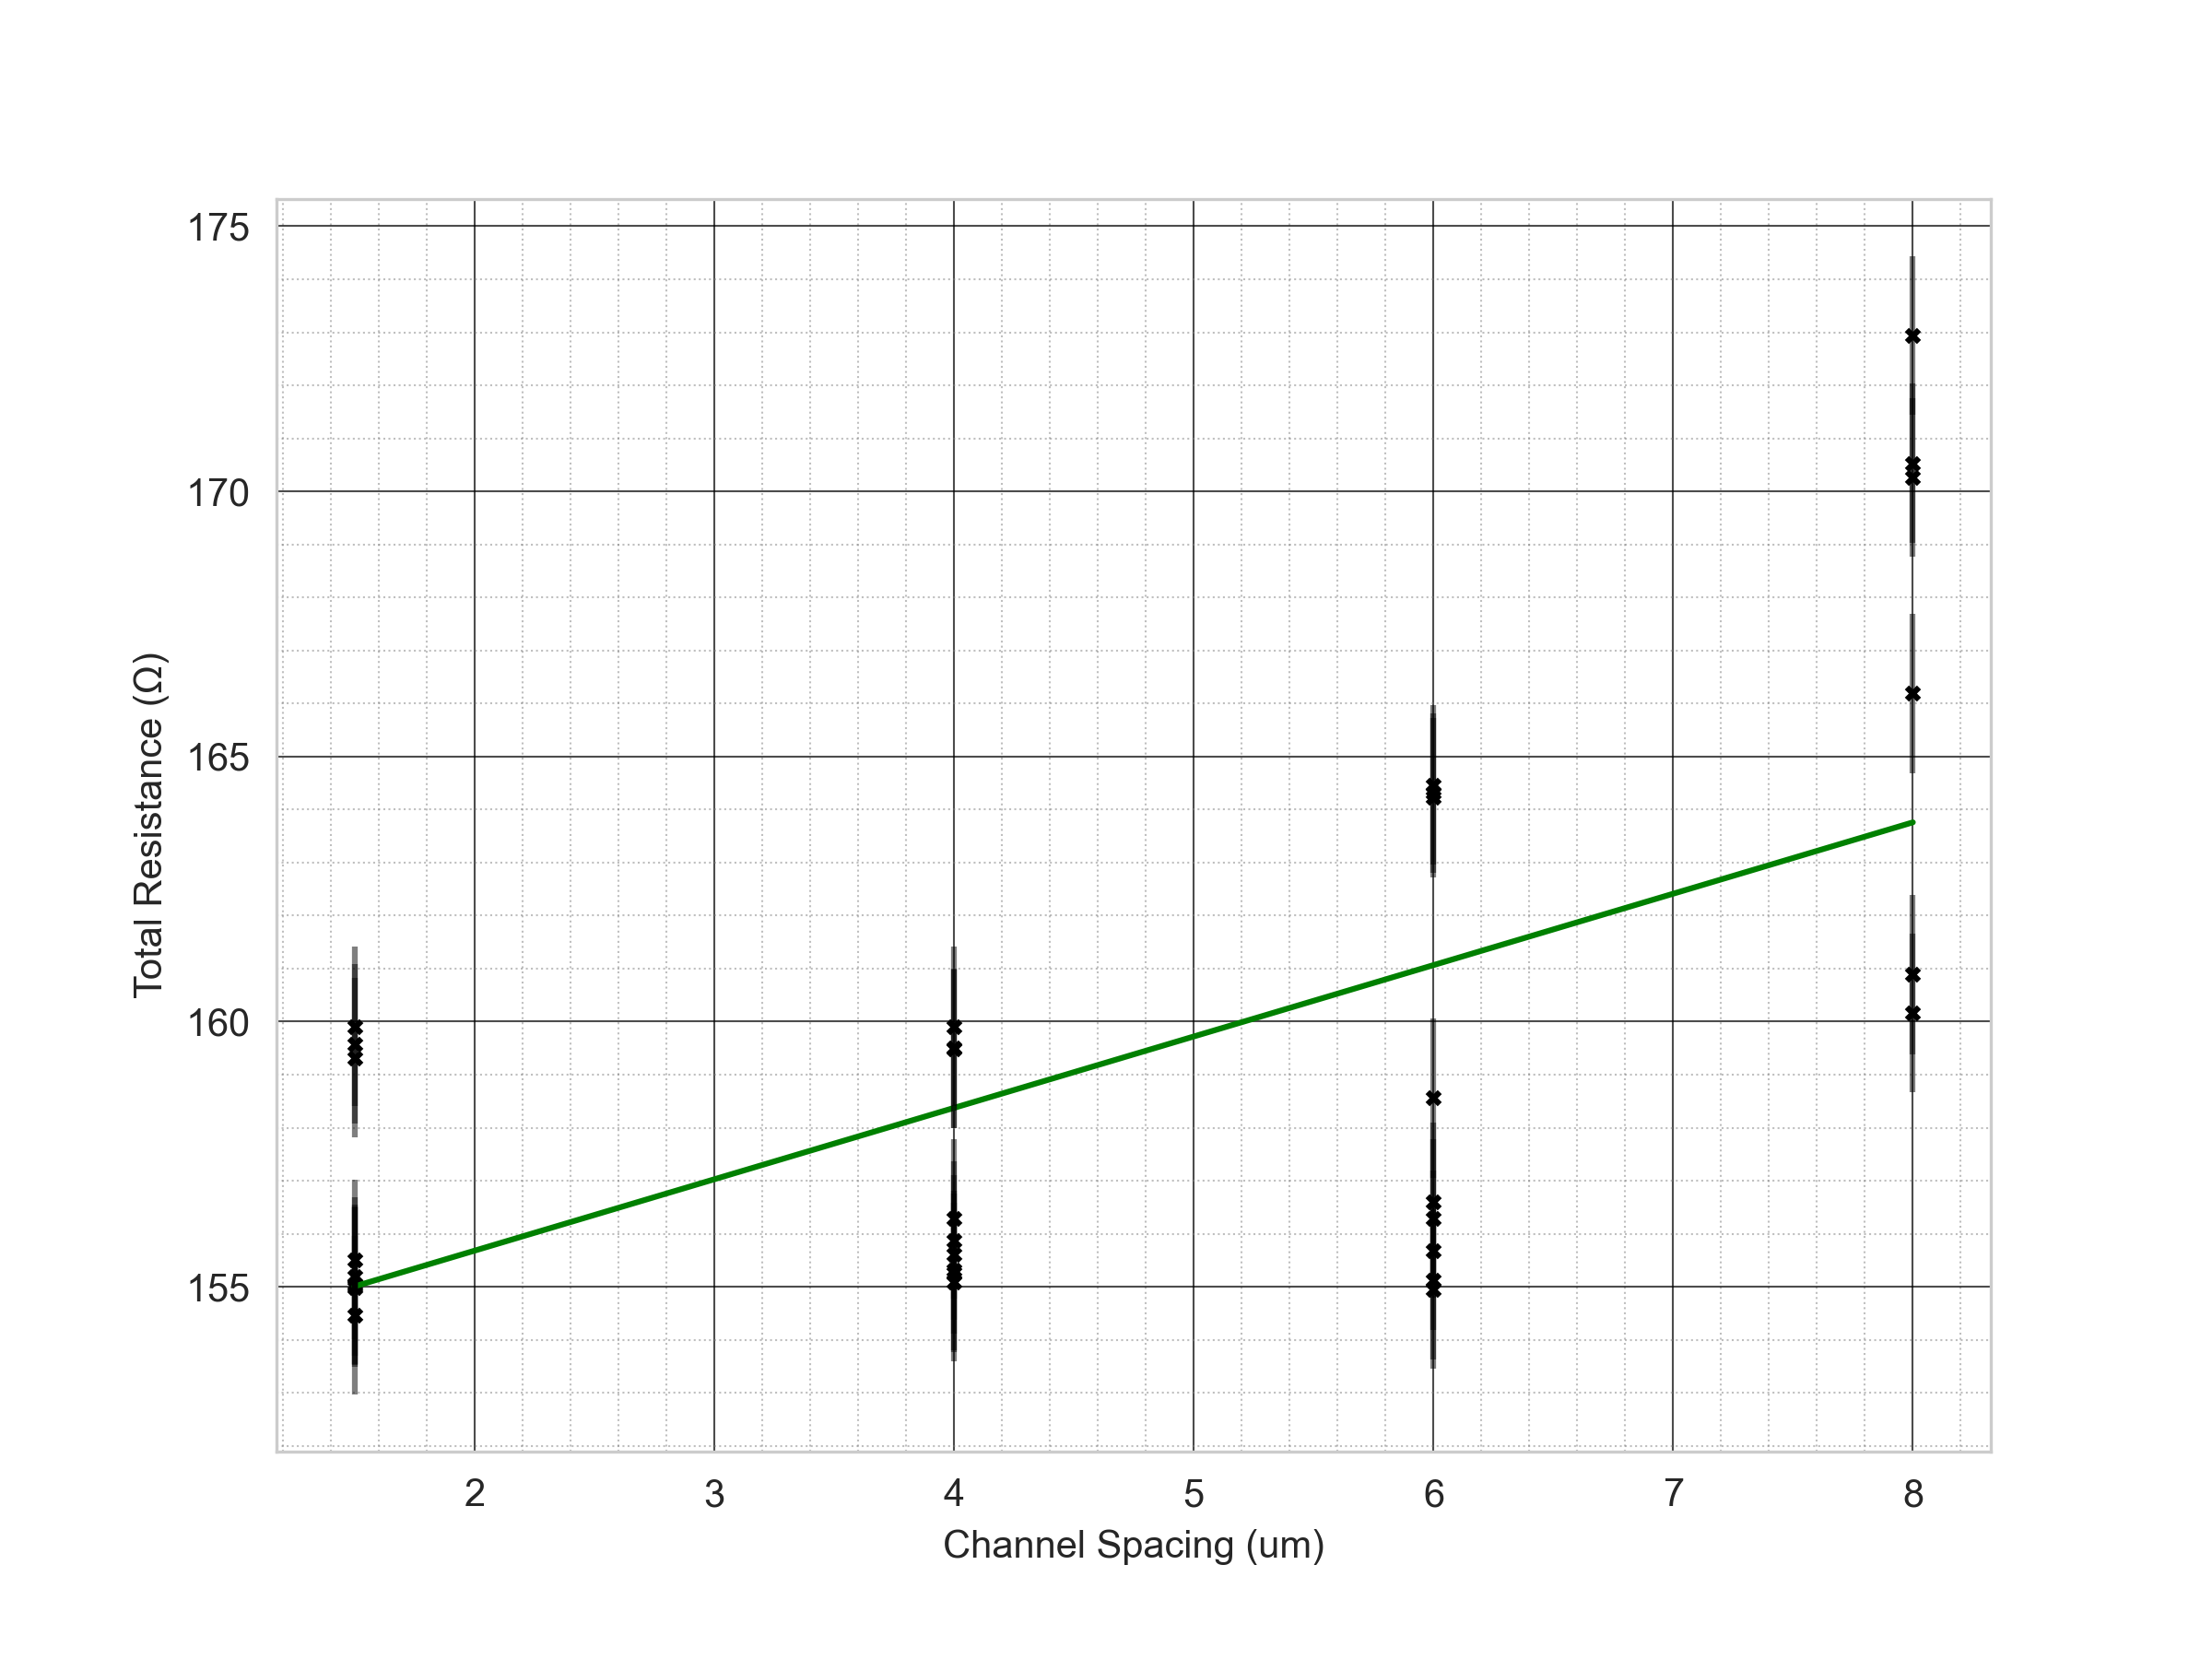
\includegraphics[width=\linewidth]{Chapter7/Figs/Raster/LTLM_graphite_mid(5.0V).png}
    \caption{A linear plot of the total measured resistance against LTLM channel spacing at 5~\si{\volt}, with a line of best fit. Error bars of $\pm$1.5~\si{\ohm} are plotted based on the spread of data observed within each set of IV sweeps, and represent a high estimate of the systematic error.}
    \label{fig:ltlm_graphite_5v_mid}
\end{figure}

Figure \ref{fig:ltlm_graphite_5v_mid} shows the results of several rounds of LTLM experiments. One notable detail is the usage of slightly different channel spacings (1.5, 4, 6, 8 \si{\micro\metre}) when compared to the designed spacings (2, 5, 7, 9 \si{\micro\metre} respectively). This reduction of channel spacing was implemented to better reflect the observed topology of laser written devices, but while the data themselves better match these spacings, this is a difficult measurement to take from the given characterisation techniques and remains as an assumption to allow for plotting. Further to this, the low total resistance observed across all channels is a challenging result to reconcile with the previous wire measurements. This will be explored further in the following sections.

Despite the linear fit seen in figure \ref{fig:ltlm_graphite_5v_mid} having an R$^{2}$ value of 0.39, the extracted specific contact resistivity is $5.5\times10^{-5}$~\si{\ohm\centi\metre\squared}, representing the lowest specific contact resistivity to highly phosphorous doped diamond of any devices presented in the literature. It is important to note the voltage at which this set of data is obtained, 5~\si{\volt}. This is a reasonable estimate of the linear, forward bias region of one of the two Schottky barriers, but the linear IV characteristics for all channel spacings reflect the lack of comparison to that of ohmic contacts around the 0~\si{\volt} region. 

\subsubsection{Line of Best Fit and LTLM Parameters}
\begin{figure}[H]
    \centering
    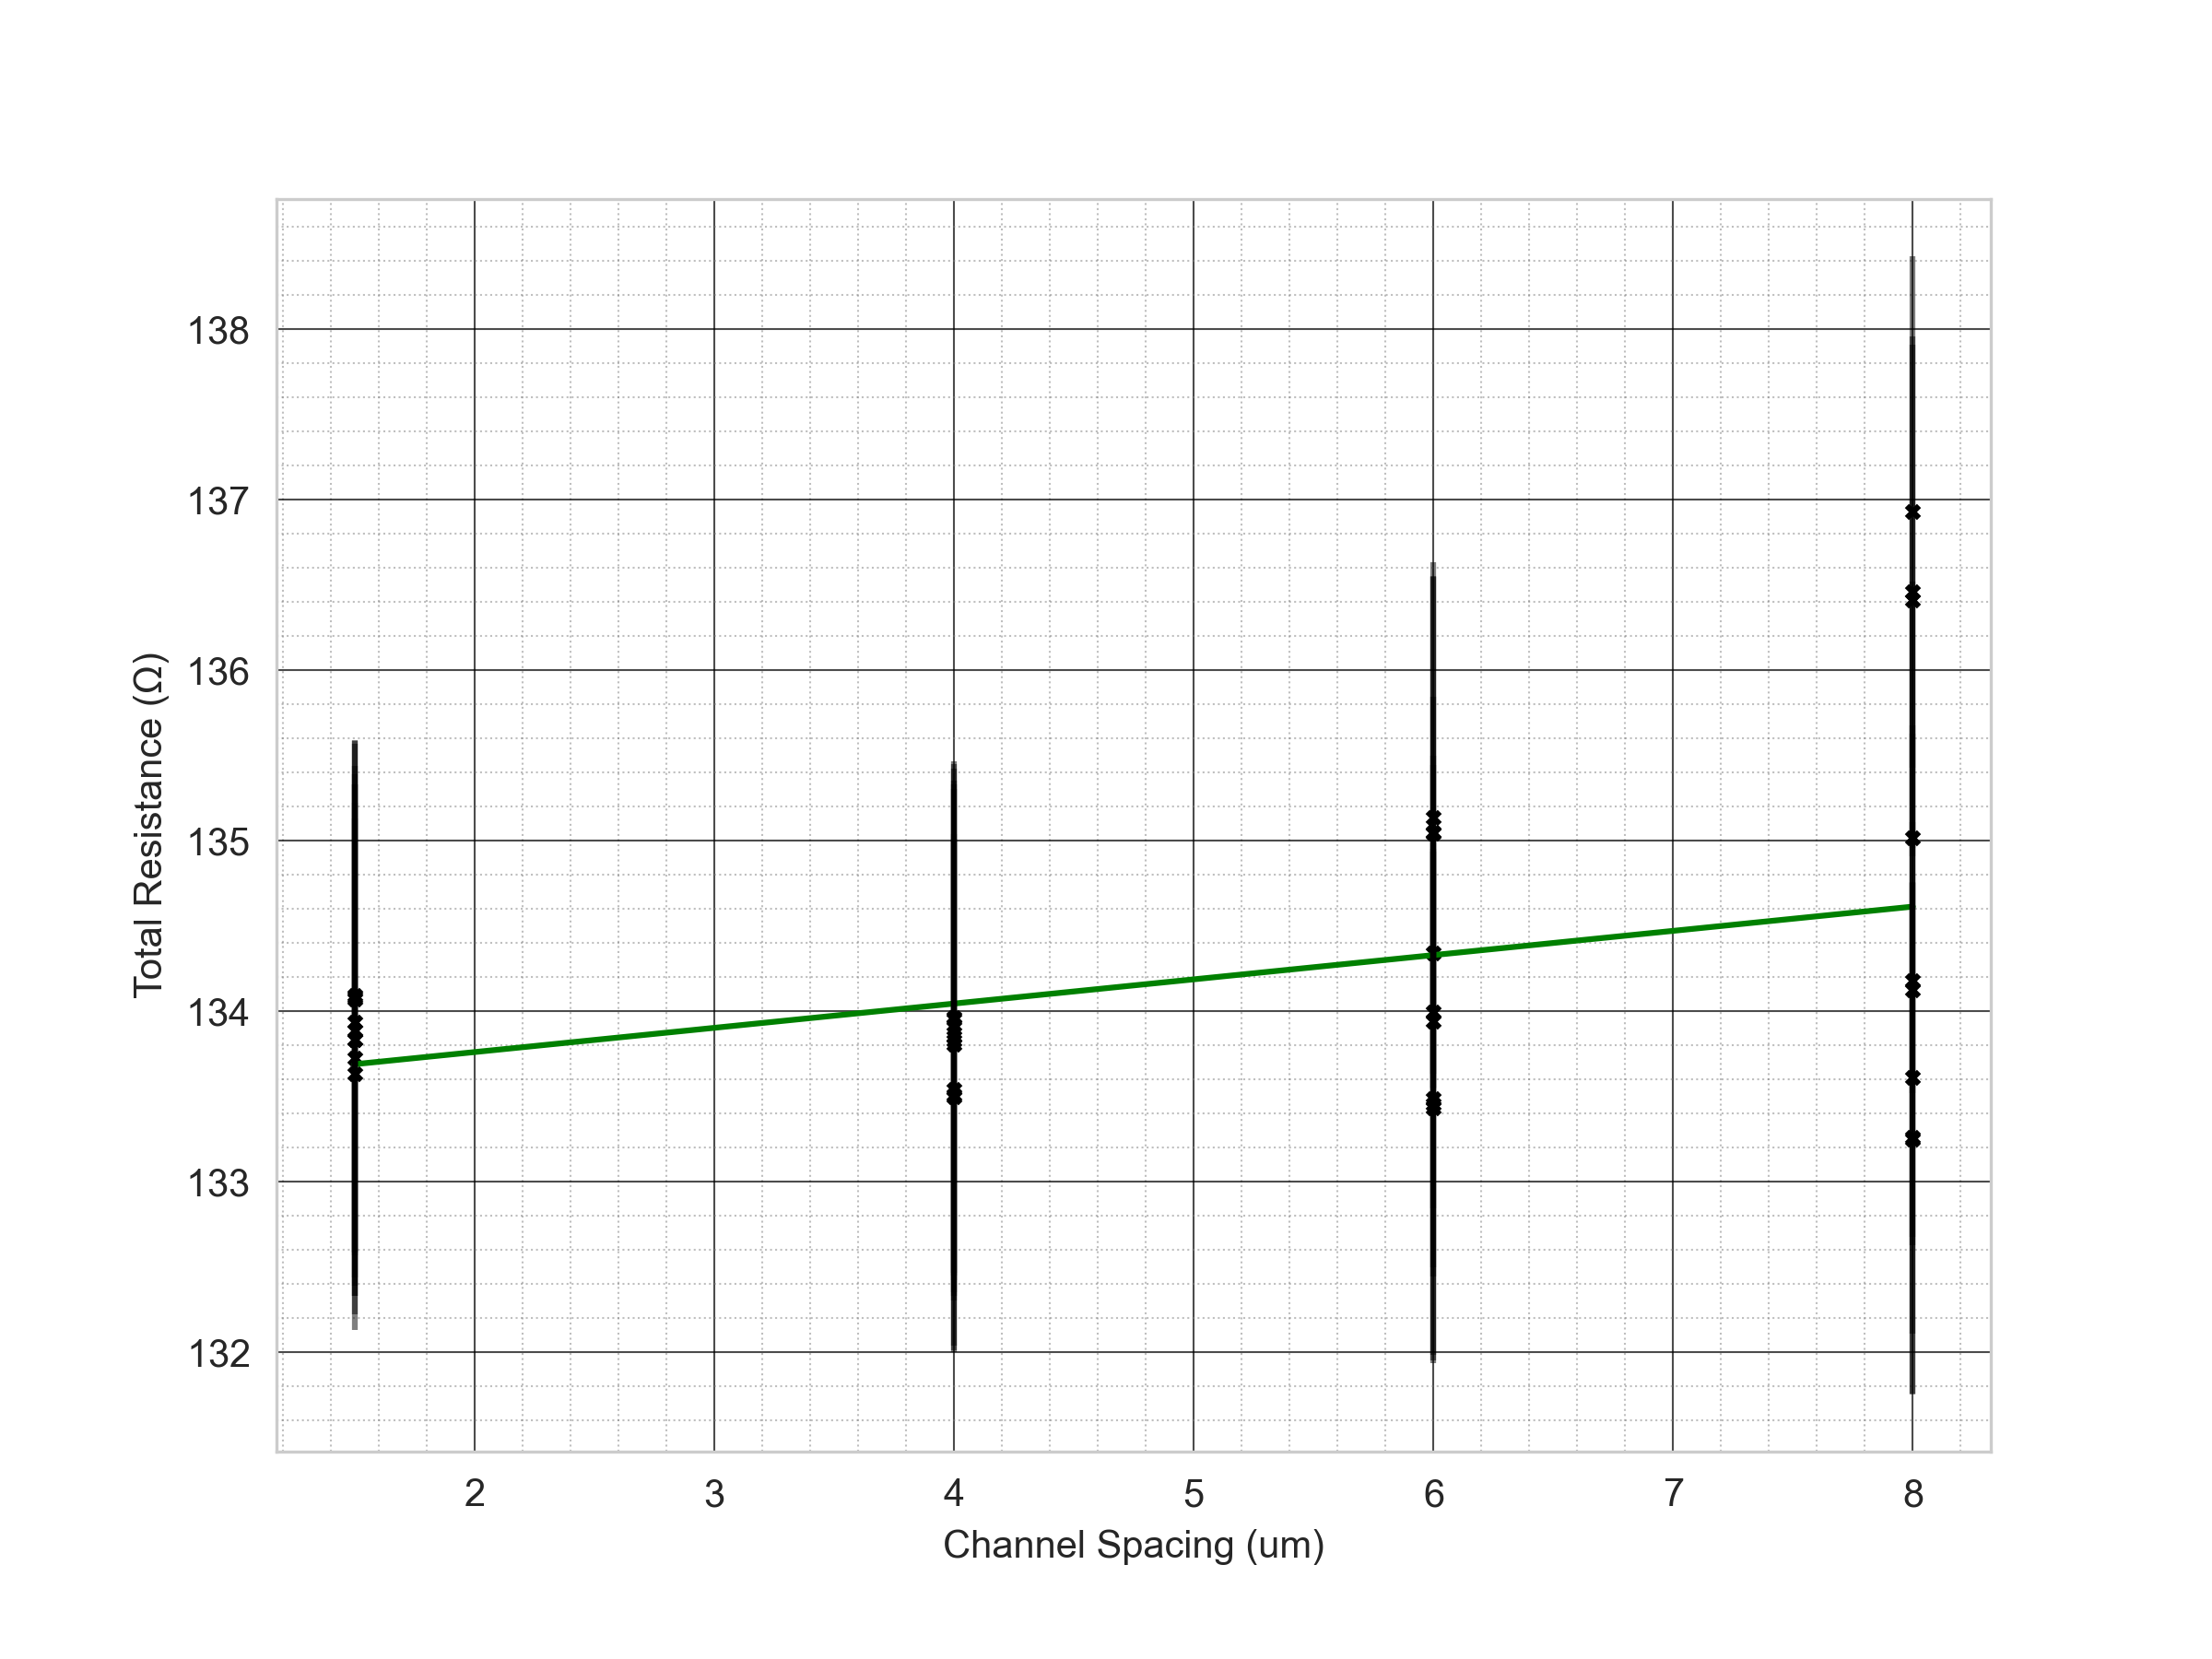
\includegraphics[width=\linewidth]{Chapter7/Figs/Raster/LTLM_graphite_mid(10.0V).png}
    \caption{A linear plot of the total measured resistance against LTLM channel spacing at 10~\si{\volt}, with a line of best fit. Error bars of $\pm$1.5~\si{\ohm} are plotted based on the spread of data observed within each set of IV sweeps, and represent a high estimate of the systematic error.}
    \label{fig:ltlm_graphite_10v_mid}
\end{figure}

Figure \ref{fig:ltlm_graphite_10v_mid} shows the LTLM plot for resistance data collected at a potential bias of 10~\si{\volt}. The line of best fit in this case is very poor, with an R$^{2}$ value of 0.15. The measured resistance has been lowered relative to the 5~\si{\volt} measurements for all channel lengths, which may be due to the voltage-dependent conductivity of laser processed wires.

As seen, when the LTLM methodology is applied to differing voltages, the resulting line of best fit can change quite dramatically in quality relative to the data. However, while the specific values of the total measured resistance do generally reduce at higher voltages, the rough trendlines observed in figures \ref{fig:ltlm_graphite_5v_mid} and \ref{fig:ltlm_graphite_10v_mid} are still present. It is also worth noting that any line which passes through the LTLM data presented here will have similar orders of magnitude for the specific contact resistivity and sheet resistance/resistivity, regardless of the resulting R$^{2}$ value. 

This allows for some speculative comparison to be made to work such as Valappil et al. \cite{valappil2022}, \cite{valappil2023}, who demonstrated nanocarbon specific contact resistivitys of $1\times10^{-3}$~\si{\ohm\centi\metre\squared} for the voltage range of 5--10~\si{\volt}. Matsumoto et al \cite{matsumoto2013} demonstrated thermally graphitised CTLM specific contact resistivitys of $0.9$~\si{\ohm\centi\metre\squared}, notably at around the 2~\si{\volt} mark. Finally, previous literature values such as that of Kato et al \cite{kato2009} at $2\times10^{-3}$~\si{\ohm\centi\metre\squared} may also be considered, though this publication did not use the constant current condition necessary for CTLM methodology.

The error present with any linear fit in figure \ref{fig:ltlm_graphite_5v_mid} prevents any conclusive comparison to be made with these examples, as a linear fit to these data is speculative at best. A useful consideration may be the range of linear fits that are possible given this dataset, as the specific contact resistivity estimation of $1\times10^{-5}$~\si{\ohm\centi\metre\squared} is two orders of magnitude lower to comparable contacts made using nanocarbon or thermally graphitised contacts on highly phosphorous doped material.

Another consideration is the possibility of the electrical contacts deteriorating over time, or with consecutive electrical measurements. The data used for figure \ref{fig:ltlm_graphite_5v_mid} spans multiple days, with repeat measurements on those days. While a good degree of repeatability was observed throughout the experimental process, the similarity between total measured resistances across the range of channels does raise questions concerning the source of any error. Although data that were likely affected by poor contact placement have already been discarded, the factor of variable conductivity within the wires themselves, and the potential impact of this upon the graphite/diamond/graphitic structure formed, is more difficult to quantify. Finally, the discrepancy between the measured resistance across LTLM contacts and the wire test structures must be considered. 

\subsubsection{Missing Resistance}
\label{subsubsec:missing_resistance}
As previously stated in section \ref{subsubsec:2um channel iv characteristics and ltlm assumptions}, the IV characteristics of the LTLM structure were performed with an observation of repeatability between differing days and across all four channel spacings. However, testing of emitter structures revealed a significantly lower base current, of the order of \si{\micro\ampere}. This is in line with the previous electrical measurements across wire testing structures in section \ref{subsec:testing_of_surface_graphitic_wires}, and hence the LTLM measurements require further exploration.

\begin{figure}[H]
    \centering
    \includegraphics[width=\linewidth]{Chapter7/Figs/Raster/All Graphitised linear IV - Data within ±20.0V_IV_plot.png}
    \caption{A linear plot of the averaged IV characteristics across all channel spacings with percentage error bars of 5\%.}
    \label{fig:all_linear_iv}
\end{figure}

\begin{wrapfigure}{r}{0.4\linewidth}
  \centering
  \includegraphics[width=\linewidth]{Chapter7/Figs/Raster/missing_resistance_circuit.png}
  \caption{A circuit diagram of the expected LTLM structure for a 4~\si{\micro\metre} channel.}
  \label{fig:missing_resistance}
\end{wrapfigure}

Figure \ref{fig:all_linear_iv} shows the full range of IV characteristics for the LTLM structure. Each channel was swept at least 12 times, ranging from $\pm1$~\si{\volt}, to $\pm20$~\si{\volt}, with the average data presented in the figure. A simplified circuit diagram of the structure, as it was tested, may resemble a series of parallel resistors, along with the channel resistor. Taking an average value of resistivity for the 10~\si{\micro\metre} wires of $0.14$~\si{\ohm\centi\metre}, and estimating the distance via the two conductive paths from the probe to the LTLM channel as 162~\si{\micro\metre}, thickness 0.5~\si{\micro\metre}, the predicted pair of resistors for each contact wire are 21~\si{\kilo\ohm}. Given a channel spacing of 4~\si{\micro\metre}, with resistivity of phosphorous doped diamond as quantified by CTLM at 15~\si{\ohm\centi\metre}, thickness 1.2~\si{\micro\metre} and contact width 60~\si{\micro\metre}, it can be expected for the channel resistance to be approximately 340~\si{\kilo\ohm}. This is represented by figure \ref{fig:missing_resistance}.

This resistance is not reflected in the LTLM data, despite further experiments on emitter structures following this expectation well. As this is the case for all LTLM data collected in this set of experiments, which involved at minimum two days of data collection, it is unclear why this is the case. The data point towards an unintended conduction channel being responsible for the observed IV characteristics, despite control experiments ensuring that no conductive channel was present without the probes actively in contact with the LTLM test structure, as is standard practice. Furthermore, the same probes and experimental setup were used to provide testing data on wire structures, with no issues identified with any of those electrical sweeps or the data in follow-up analysis. Despite these checks, the LTLM data presented here must be considered to be affected by a systematic error, due to the large discrepancy in observed resistance and the resistance of all other test structures.

Finally, with the benefit of additional data through emitter testing and another LTLM experiment that will be presented in the following sections, a more realistic peak current value may be expected at the 3~\si{\micro\ampere} level for channel spacings comparable to that of the LTLM structure. While this is certainly not a full TLM methodology, if the current observed in all of the LTLM measurements presented here were affected by a factor of $10^{5}$ shift due to an unknown systematic error, then the actual specific contact resistivity would be approximately 1~\si{\ohm\centi\metre\squared}. This is the same order of magnitude that was observed via thermal graphitisation \cite{matsumoto2013}, and would place laser processing firmly among the established methods of reducing specific contact resistivity to highly phosphorous doped diamond, even given the lower resistivity previously measured on these samples using CTLM which will make any ohmic contacts harder to form. 

\subsection{Second Round Of LTLM}
\label{subsec:ltlm2_lost_data}
As it was established in section \ref{subsubsec:missing_resistance} that the collected LTLM data had an inexplicable systematic error following measurements of emitter structures, a fresh set of measurements were taken with new micro-probes and another solvent clean. To ensure that these data would have a higher reliability, the additional step of taking measurements under illumination and in complete darkness was undertaken. The intention of this, along with a more thorough experimental process overall was to ensure that the IV data was both repeatable and also sensible in the context of phosphorous doped diamond samples.

\subsubsection{IV Characteristics (Light/Dark)}

\begin{figure}[H]
    \centering
    \includegraphics[width=\linewidth]{Chapter7/Figs/Raster/Lost Data/20V Combined IV Characteristics for All Conditions.png}
    \caption{A linear plot of the averaged IV characteristics across all channel spacings, $\pm20$~\si{\volt}, under bright illumination or in darkness.}
    \label{fig:lost_iv_20v}
\end{figure}

Figure \ref{fig:lost_iv_20v} shows the full set of IV characteristics taken during this second run of LTLM measurements. Each set of scatter points represents 3 datasets, averaged together with 501 data points. The same probe positions as for the previous LTLM measurements were used. Lighter and darker colours are used to help provide a visual difference between the light and dark datasets respectively, which diverge in a consistent manner. The reduction of measured total resistance under illumination provides a clear indication of semiconducting properties, with the conductive path expected to be within the phosphorous doped diamond surface layer. The observed current matches the conclusions drawn from the previous LTLM testing, with the correct order of magnitude as expected for contacts of $\sim1$~\si{\ohm\centi\metre\squared} beyond the low voltage region. Note that in contrast to the previous LTLM IV plots which had 5\% error bars to account for the spread of datapoints observed during testing, the data in this figure were observed to be highly repeatable and the error can instead be presumed to be close to the limit imposed by that of the B1500 probe station. As calibrated, this is below $1$~\si{\nano\ampere}, approaching $1$~\si{\pico\ampere}, and is hence not visible in the plots of currents as error bars.

\begin{figure}[H]
    \centering
    \includegraphics[width=\linewidth]{Chapter7/Figs/Raster/Lost Data/5V Combined IV Characteristics for All Conditions.png}
    \caption{A linear plot of the averaged IV characteristics across all channel spacings, $\pm5$~\si{\volt}, under bright illumination or in darkness.}
    \label{fig:lost_iv_5v}
\end{figure}

In figure \ref{fig:lost_iv_5v}, the low voltage region in particular is plotted. At this scale, it is difficult to see the marginal reduction in resistance due to illumination relative to the dark characteristics. It is also considered that the 501 datapoints used for these sweeps are adequate to resolve the low voltage region, which may be defined as $\pm1$~\si{\volt}. Further sampling would provide more certainty for comparisons between channels, but the potential for error due to micro-probe positioning negates the slight gains in precision that could be obtained with higher datapoints. Within this bias region, neither of the double Schottky barriers are sufficiently biased to overcome the Schottky barrier heights. As for figure \ref{fig:lost_iv_20v}, the channels are ordered in measured resistance as should be expected, 2-1, 3-2, 4-3 and 5-4, in order of ascending channel spacings.

\subsubsection{LTLM Characteristics (Light/Dark)}

\begin{figure}[H]
    \centering
    \includegraphics[width=\linewidth]{Chapter7/Figs/Raster/Lost Data/LTLM_graphite_mid(20V).png}
    \caption{A LTLM plot of the total measured resistance against LTLM channel spacing at 20~\si{\volt}, with lines of best fit for both the illuminated and dark datasets. Uncertainties due to the error associated with current measurements are not possible to see at this scale, $\pm0.5$~\si{\micro\metre} horizontal error bars are plotted.}
    \label{fig:lost_ltlm_20v}
\end{figure}

\begin{table}[h!]
\centering
\begin{tabular}{|c|c|c|}
\hline
\textbf{Parameter} & \textbf{Light} & \textbf{Dark} \\
\hline
R$^{2}$ & 0.969 & 0.966 \\
\hline
$R_{c}$ (\si{\kilo\ohm}) & $915$ & $949$ \\
\hline
$R_{s}$ (\si{\mega\ohm\per\sq]}) & $35.9$ & $37.7$ \\
\hline
$\rho_{c}$ (\si{\ohm\centi\meter\squared}) & 0.659 & 0.683 \\
\hline
$L_{t}$ (\si{\micro\meter}) & 1.53 & 1.51 \\
\hline
$\rho_{s}$ (\si{\ohm\centi\meter}) & 4300 & 4530 \\
\hline
\end{tabular}
\caption{LTLM Parameters at 20~\si{\volt} for light and dark conditions.}
\label{tab:lost_ltlm_parameters_20v}
\end{table}

Figure \ref{fig:lost_ltlm_20v} shows the results of plotting the total measured resistance at 20~\si{\volt} against the designed channel spacing (2, 5, 7 and 9~\si{\micro\metre}), with the data taken both under a bright light source and also in complete darkness represented. Error bars of $\pm0.5$~\si{\micro\metre} are plotted to account for the possible deviation of channel spacing as observed via optical characterisation. The extracted parameters are summarised in table \ref{tab:lost_ltlm_parameters_20v}.

\begin{figure}[H]
    \centering
    \includegraphics[width=\linewidth]{Chapter7/Figs/Raster/Lost Data/LTLM_graphite_mid(5V).png}
    \caption{A LTLM plot of the total measured resistance against LTLM channel spacing at 5~\si{\volt}, with lines of best fit for both the illuminated and dark datasets. Uncertainties due to the error associated with current measurements are not possible to see at this scale, $\pm0.5$~\si{\micro\metre} horizontal error bars are plotted.}
    \label{fig:lost_ltlm_5v}
\end{figure}

\begin{table}[h!]
\centering
\begin{tabular}{|c|c|c|}
\hline
\textbf{Parameter} & \textbf{Light} & \textbf{Dark} \\
\hline
R$^{2}$ & 0.978 & 0.976 \\
\hline
$R_{c}$ (\si{\kilo\ohm}) & $2244$ & $2268$ \\
\hline
$R_{s}$ (\si{\mega\ohm\per\sq}) & $49.5$ & $49.9$ \\
\hline
$\rho_{c}$ (\si{\ohm\centi\meter\squared}) & 1.62 & 1.63 \\
\hline
$L_{t}$ (\si{\micro\meter}) & 2.72 & 2.73 \\
\hline
$\rho_{s}$ (\si{\ohm\centi\meter}) & 5940 & 5990 \\
\hline
\end{tabular}
\caption{LTLM Parameters at 5~\si{\volt} for light and dark conditions.}
\label{tab:lost_ltlm_parameters_5v}
\end{table}

Figure \ref{fig:lost_ltlm_5v} shows a LTLM plot for total resistance as measured at an applied bias of 5~\si{\volt} against the designed channel spacing (2, 5, 7 and 9~\si{\micro\metre}), with the data taken under both a bright light source and also in complete darkness represented. Error bars of  $\pm0.5$~\si{\micro\metre} are plotted to account for the possible deviation of channel spacing as observed via optical characterisation. The extracted parameters are given in table \ref{tab:lost_ltlm_parameters_5v}. The change in specific contact resistivity is quite natural, as it may be interpreted as mostly being due to the image force barrier lowering of the forwardly biased Schottky barrier in the double Schottky structure \cite{sze2006}, \cite{Aubry1994}. There is the additional factor of greater donor ionisation under increasing electric field strengths that may also be considered as a factor, since the majority of substitutional phosphorous dopants are effectively frozen out at room temperature \cite{koizumi1997}, \cite{Donato2018}, \cite{donato2019}. The concentration of dopants is a key factor in the formation of conventional ohmic contacts on semiconductors, and this may hence be visible here.

\subsubsection{Voltage Dependent specific contact resistivity}

\begin{figure}[H]
    \centering
    \includegraphics[width=\linewidth]{Chapter7/Figs/Raster/Lost Data/LTLM_rhoc_plot.png}
    \caption{A plot of the measured specific contact resistivity as a function of applied voltage, sampling the full range of IV characteristics.}
    \label{fig:lost_ltlm_rhoc}
\end{figure}

Finally, figure \ref{fig:lost_ltlm_rhoc} provides a visual representation for the dependence of specific contact resistivity upon the applied voltage across the device. Notably, even in the very low voltage region approaching 0~\si{\volt}, the specific contact resistivity remains below 20~\si{\ohm\centi\metre\squared}. This is quite unexpected, as the IV characteristics would initially indicate that the low voltage region has a very high resistance. Instead, it is clear that the double Schottky structure here allows for a measurable level of leakage current even without either contact being in the forward bias mode of operation. The difference between measurements taken under direct illumination and in complete darkness are difficult to pick apart in figure \ref{fig:lost_ltlm_rhoc}, but there is a mean difference between the light and dark data of $-0.0228$~\si{\ohm\centi\metre\squared}, with a variance of $0.0003$~\si{\ohm\squared\centi\metre\tothe{4}}. The negative mean difference indicates that the dark specific contact resistivity is higher than that of the well lit measurements, and the variance is low enough to consider the majority of data in this voltage range to agree with this mean difference. For a final check, a comparison between all pairs of datapoints was conducted to find any dark values which were less than that of the light measurements. All such values are contained within the $\pm1.08$~\si{\volt} range, as could be expected based on the divergence of IV characteristics beyond 1~\si{\volt}.

Throughout all of the data presented for the second round of LTLM measurements, the error can be estimated via the previously discussed estimates of error via exact probe positioning on the laser processed wires. The systematic error present for these measurements is estimated to be approaching the limit imposed by the B1500 probe station, which is well below even 1\% of the currents measured here.

Before examining the emitter structures designed to take advantage of geometrically enhanced field effect emitters, at this point it is necessary to consider theoretical models of the double Schottky device structure, which may also be described as a back-to-back Schottky junction. This will provide the necessary framework for understanding the difference between thermionic and field effect emission characteristics.\end{comment}

\section{Laser Graphitised Emitters}
As discussed in section \ref{subsec:field_effect_emission}, laser processing with the aim of producing graphitised wires on the surface or within the bulk of diamond may be used to fabricate devices that rely upon geometric enhancement and hence field effect emission. Simulations produced by the candidate indicated that an appreciable level of Fowler-Nordheim type tunnelling is feasible with the small dimensions of laser fabricated wires in diamond \cite{sun2014}. Hence, to test this prediction experimentally, arrays of sharp emitters were designed in a similar fashion to that of LTLM contacts, to provide direct reference data to check for the presence of field effect emission current contributions.
\subsection{Microscopy of Emitters Prior to Testing}
\begin{figure}[H]
    \centering
    \includegraphics[width=\linewidth]{Chapter7/Figs/Raster/emitter_overview_fl.jpg}
    \caption{An overview of the emitter array structures via confocal microscopy with 488~\si{\nano\metre} laser illumination and 408~\si{\nano\metre} fluorescence.}
    \label{fig:emitter_fl}
\end{figure}

In figure \ref{fig:emitter_fl}, the fluorescence imaging has been cropped to better display the observed fluorescence of these structures. Red circles are used to highlight fluorescence which has previously been determined to be that of surface contaminants. Please see section \ref{subsec:fluorescence_characterisation} for the full analysis of fluorescence characterisation.

\begin{figure}[H]
    \centering
    \includegraphics[width=\linewidth]{Chapter7/Figs/Raster/ch_channel_esid.jpg}
    \caption{A cropped view of the CH emission channel, as seen via confocal microscopy with 488~\si{\nano\metre} laser illumination.}
    \label{fig:ch_esid}
\end{figure}

\begin{figure}[H]
    \centering
    \includegraphics[width=\linewidth]{Chapter7/Figs/Raster/ch_channel_fl.jpg}
    \caption{A cropped view of the CH emission channel, as seen via confocal microscopy with 488~\si{\nano\metre} laser illumination and 408~\si{\nano\metre} fluorescence.}
    \label{fig:ch_fl}
\end{figure}

\begin{figure}[H]
    \centering
    \includegraphics[width=0.8\linewidth]{Chapter7/Figs/Raster/ch_design2.png}
    \caption{The designed channel of emitter channel CH, with measurements of all features.}
    \label{fig:ch_design}
\end{figure}

Figures \ref{fig:ch_esid} and \ref{fig:ch_fl} show the confocal microscopy when cropped down to only the relevant channel, without and with fluorescence respectively. The emitter tip profiles are observed to follow the approximations used in modelling, with the exact radius of curvature for the effective rectangular corners appearing to only show a small amount of variation. Figure \ref{fig:ch_design} shows the designed structure of this channel, with emitter wires of thickness 0.8~\si{\micro\metre} chosen in large part due to the enhanced conductivity for slightly wider wire geometries as demonstrated in previous work by Oxford \cite{sun2014}, and also as recommended in consultations with Patrick Salter and Ravi Shivaraman. Thinner wires with a lower conductivity may have a greater geometric enhancement factor, but will ultimately be dependent upon the local, possibly quite high resistivities. 

As has been discussed in the previous trial wire measurements from section \ref{subsec:testing_of_surface_graphitic_wires}, some discrepancy even within wide contact wires has been observed that may indicate a difference in sp$^{2}$ conductive carbon allotropes as generated by laser processing on this sample. The difference in observed emitter profiles hence is not unusual, as the exact profile of laser-induced change in carbon allotropes may be highly sensitive to local crystallinity, which is certainly a factor for the phosphorous-doped surface layer on this sample.

Finally, the fluorescence observed in figure \ref{fig:ch_fl} for emitter array CH has a few notable distinguishing features. First is the bright spot on the apex of the second emitter from the left. This may simply be a surface contaminant, or it may originate from the laser processed carbon. Second is the notable patches along the edges of the contacts. 

\begin{figure}[H]
    \centering
    \includegraphics[width=0.8\linewidth]{Chapter7/Figs/Raster/CH_cropped_overlay.jpg}
    \caption{An overlay of the fluorescence observed in channel CH with the AFM topology.}
    \label{fig:ch_overlay}
\end{figure}

Figure \ref{fig:ch_overlay} attempts to visually compare the AFM topology with that of the fluorescence observed. While this is perhaps a difficult comparison to infer meaning from, the two regions where there is a lack of ablation relative to surrounding laser processed diamond on contact H stand out as noteworthy material with a visible fluorescence.

\subsubsection{Possible Impact of Surface Topology on Emitter Profiles - HIM}

\begin{figure}[H]
    \centering
    \includegraphics[width=\linewidth]{Chapter7/Figs/Raster/him 002 A.1.jpg}
    \caption{Helium ion microscopy of sample F, as was used for Ti/Au CTLM measurements. Performed in collaboration with NEXUS - Surface characterisation facility at Faculty of SAGE.}
    \label{fig:him_1}
\end{figure}

To further underscore the crystallinity factor of laser processing and how it may impact the resulting profile of laser induced allotrope changes on the micro-scale, figure \ref{fig:him_1} shows a sample of HIM that was performed on sample F following CTLM characterisation. This figure is of the highly phosphorous doped diamond surface, which is grown with the same parameters as sample G - the laser processed substrate, with no metal present on this part of the sample. On the scale of $\sim200$~\si{\nano\metre}, multiple "islands" of diamond growth can be seen, corresponding to highly disordered diamond growth with significant concentrations of twinning defects which are typical for \hkl(111) oriented samples \cite{Butler2007}, \cite{prelas:1997}, \cite{koizumi1997}, \cite{koizumi2000}, \cite{Shechtman1993}. 

It is slightly speculative to comment on the possible role of twinning boundaries and the modification of carbon allotropes via laser processing, but based on the size and shape of these islands, it may be the case that the exact emitter profile is dependent upon the local islands within the emitter channel. This would align with theoretical work into the origin of photographitisation processes being primarily defective sites in the diamond lattice \cite{Kononenko2009}, \cite{kononenko:2015}, but it is unclear on how this may relate to the more recent work on diaphitic allotropes of carbon \cite{salter2024}, \cite{Nemeth2020}, \cite{Nemeth20202}, \cite{Nemeth2021}. Field effect emission from polycrystalline films are a well studied portion of diamond electronic devices \cite{Sugino1998}, \cite{Watanabe2001}, \cite{Watanabe2003}, and in particular the internal boundary of phosphorous doped polycrystalline diamond emitters has also been studied previously \cite{Sugino19982}, hence the impact of a relatively polycrystalline surface layer of highly phosphorous doped diamond may be beneficial in the production of high geometric field enhancement, despite the difficulty in producing designs that rely upon planar geometries for exact device properties.

\begin{figure}[H]
    \centering
    \includegraphics[width=\linewidth]{Chapter7/Figs/Raster/him 007 A.6.jpg}
    \caption{Helium ion microscopy of sample F, as was used for Ti/Au CTLM measurements. Performed in collaboration with NEXUS - Surface characterisation facility at Faculty of SAGE.}
    \label{fig:him_2}
\end{figure}

Figure \ref{fig:him_2} provides another HIM scan of sample F, but with a much smaller scan area of only 1.5~\si{\micro\metre} in comparison to the previous FOV of 8~\si{\micro\metre}. Note the marked region on the left is a Ti/AU contact, while the right side is the uncoated phosphorous doped diamond surface, which displays a complex surface topology on the scale of tens of nanometres to hundreds of nanometres.

\subsubsection{Possible Impact of Surface Topology on Emitter Profiles - D-AFM and NC-AFM}
One extra set of topology characterisation data was taken via dynamic-AFM or tapping mode AFM on an untreated region of sample G, to provide some certainty that the heavily phosphorous doped surface layer grown on the two samples is indeed similar in crystallinity. Unfortunately, the only cantilevers accessible for use in this endeavour were the NC-AFM tips as used for the earlier AFM topologies. While the z axis resolution for previous scans was suitable to detect the surface ablation for emitter wires of width 0.8~\si{\micro\metre} and other such features, the diamond surface required an order of magnitude improvement. Hence, measurements were conducted with a wide sweep of the available adjustable parameters for the XE-150 AFM system, in an attempt to achieve the required resolution with cantilevers that are not suitable for contact-AFM mode characterisation.

\begin{figure}[H]
    \centering
    \begin{subfigure}[b]{0.49\textwidth}
        \centering
        \includegraphics[width=\textwidth]{Chapter7/Figs/Raster/DAFM/forward DFM 55 drive 2 z 256 04 Hz.png}
        \caption{D-AFM scan.}
        \label{fig:dafm}
    \end{subfigure}
    \hfill
    \begin{subfigure}[b]{0.49\textwidth}
        \centering
        \includegraphics[width=\textwidth]{Chapter7/Figs/Raster/DAFM/forward NC-AFM 100 drive 1 z 256 05 Hz.png}
        \caption{Finely calibrated NC-AFM scan.}
        \label{fig:ncafm}
    \end{subfigure}
    \caption{Comparison of D-AFM and NC-AFM scans of the phosphorous doped diamond surface, in a region that was not subject to laser processing.}
\end{figure}

Figures \ref{fig:dafm} and \ref{fig:ncafm} represent the best results of this topological testing conducted by the candidate. Note that the images are slightly offset due to difficulties with scanning precisely the same region on a region of the diamond sample with no visible surface features. While the HIM images demonstrate a much greater visual clarity on the nano-scale, D-AFM and NC-AFM conducted on a part of the phosphorous doped diamond surface for sample G confirm that there are indeed small islands with heights of up to around 140~\si{\nano\metre} in places. While the resolution of these images is still lacking in comparison to HIM, the randomly seeded nature of the as grown diamond surface is clear, with some quantification of the difference in height due to these different islands of diamond growth. Of the two contact methodologies employed, the tapping D-AFM mode should provide a marginally more reliable and precise topological map than the NC-AFM mode, however in this case it is hard to distinguish the two methodologies due to the calibration steps taken to reduce noise to an absolute minimum in the NC-AFM mode. Specifically, an absolute minimum level of z-drive was used, with a scan rate of 0.4~\si{\hertz} for both D-AFM and NC-AFM over a resolution of 256x256 pixels corresponding to 78~\si{\nano\metre\squared\per\pixel}. Additionally, several rounds of calibration were performed to reduce any noise due to slight mirror misalignments or other such physical parameters. The only distinguishing detail in favour of D-AFM may be the observation of lower average troughs, which should reflect directly on the AFM tip relying on the tipping point of attractive and repulsive Van der Waals forces to identify the correct local heights.

\subsection{Emitter Electrical Characteristics}

\begin{figure}[H]
    \centering
    \includegraphics[width=\linewidth]{Chapter7/Figs/Raster/emitter_probes_esid.jpg}
    \caption{An overview of the emitter array structures via confocal microscopy with 488~\si{\nano\metre} laser illumination, and the locations of specific probes during IV characterisation of channel CH.}
    \label{fig:emitter_esid_anno}
\end{figure}

Figure \ref{fig:emitter_esid_anno} provides a view of the relevant emitter contact structures, and their neighbouring contacts as seen with confocal microscopy. Annotations indicating probe positions 1-4 are used for the wire verification data, and positions a-b were used for the high voltage emitter testing.

In the following sections, the verification trials undertaken to ensure good electrical contact to the laser processed wires are summarised. In essence, the core trials involved a brief IV sweep of a portion of each contact, followed by low voltage checks across the emitter channel itself to verify the correct expected orders of magnitude in resistance. 

\subsubsection{Low-Voltage Wire Testing: 4-3}

\begin{figure}[H]
    \centering
    \includegraphics[width=\linewidth]{Chapter7/Figs/Raster/Emitters/43 3x 10V.png}
    \caption{The average electrical characteristics between probe positions 4 and 3.}
    \label{fig:e_43_10v}
\end{figure}

\begin{table}[h!]
\centering
\begin{tabular}{|c|c|c|c|c|}
\hline
\textbf{Voltage (V)} & \textbf{Resistance (\si{\mega\ohm})}  & \textbf{Resistivity (\si{\ohm\centi\metre})} & \textbf{Conductivity (\si{\siemens\per\metre})} \\
\hline
10 & $0.166$ & $2.08$ & 48.2 \\
\hline
\end{tabular}
\caption{Extracted wire parameters for wire 4-3, $\pm10$~\si{\volt} measurements.}
\label{tab:43_e_wire_parameters_10v}
\end{table}

Figure \ref{fig:e_43_10v} shows the electrical characteristics as measured with probe positions 4-3 on the top of contact C. This is very roughly a measurement of the wire at the top of contact C, since the resistance of the longer wire path will have a resistance at least 3 times higher. 401 data points across 3 separate $\pm10$~\si{\volt} sweeps, with assumptions as used in the characterisation of trial wires in section \ref{subsec:testing_of_surface_graphitic_wires} are used to provide estimated wire properties as summarised in table \ref{tab:43_e_wire_parameters_10v}.

\subsubsection{Low-Voltage Wire Testing: 2-1}
\begin{figure}[H]
    \centering
    \includegraphics[width=\linewidth]{Chapter7/Figs/Raster/Emitters/21 3x 10V.png}
    \caption{The average electrical characteristics between probe positions 2 and 1.}
    \label{fig:e_21_10v}
\end{figure}

\begin{table}[h!]
\centering
\begin{tabular}{|c|c|c|c|c|}
\hline
\textbf{Voltage (V)} & \textbf{Resistance (\si{\mega\ohm})}  & \textbf{Resistivity (\si{\ohm\centi\metre})} & \textbf{Conductivity (\si{\siemens\per\metre})} \\
\hline
10 & $0.197$ & $2.46$ & 40.6 \\
\hline
\end{tabular}
\caption{Extracted wire parameters for wire 2-1, $\pm10$~\si{\volt} measurements.}
\label{tab:21_e_wire_parameters_10v}
\end{table}

Figure \ref{fig:e_21_10v} provides the electrical characteristics for the wire between probe positions 2-1 on contact H. The extracted parameters are summarised in table \ref{tab:21_e_wire_parameters_10v}. This wire shows a slightly higher effective resistivity than the wire between 4-3, but is otherwise reasonably similar in properties. Both wires are an order of magnitude lower in conductivity than the 10~\si{\micro\metre} wires tested in section \ref{subsubsec:graphitised_wire_testing_10}, which may indicate some local variation in the diamond substrate affecting the written wires between these two regions. The differential resistance in figure \ref{fig:e_21_10v} is notably scattered over a wider range of values than that of figure \ref{fig:e_43_10v}, but again the rise in resistance around a bias of 0~\si{\volt} is not as pronounced as in the case of data with a clear Schottky behaviour, and the scatter only shows a slightly non-ohmic behaviour for these wires.

\subsubsection{Low-Voltage Emitter Testing: 4-2}
Before switching the probe positions to that of a-b, measurements were taken with the 4 probe positions as for the wire testing, which provides a first look at the IV characteristics of this emitter array.
\begin{figure}[H]
    \centering
    \includegraphics[width=\linewidth]{Chapter7/Figs/Raster/Emitters/42 3x 10V.png}
    \caption{The average electrical characteristics between probe positions 4 and 2.}
    \label{fig:e_42_10v}
\end{figure}

\begin{table}[h!]
\centering
\begin{tabular}{|c|c|c|c|c|}
\hline
\textbf{Voltage (V)} & \textbf{Resistance (\si{\mega\ohm})}  & \textbf{Resistivity (\si{\ohm\centi\metre})} & \textbf{Conductivity (\si{\siemens\per\metre})} \\
\hline
10 & $6.86$ & $85.7$ & 1.17 \\
\hline
\end{tabular}
\caption{Extracted wire parameters for "wire" approximation of 4-2, $\pm10$~\si{\volt} measurements.}
\label{tab:42_e_wire_parameters_10v}
\end{table}

Figure \ref{fig:e_42_10v} presents the low voltage measurements taken across probe positions 4-2, with table \ref{tab:42_e_wire_parameters_10v} providing estimated values for the resistivity using the 10~\si{\micro\metre} wire approximation for direct comparison to previous results. This approximation is useful for comparing orders of magnitude, but since the channel resistivity will be the dominant factor, the wire dimensions approximation merely shows that the electrical data does indeed reflect the emitter channel under testing. The IV characteristics here resemble that of the LTLM channels tested in section \ref{subsec:ltlm2_lost_data}, which is a reassuring comparison, as at this potential bias the expected maximum electric field norm on emitter tips is of the order of (come back to this duh). Hence, with a low applied potential difference, the expectation is for the measured current to be due to thermionic emission.

\subsubsection{Low-Voltage Emitter Testing: a-b Ramp-Up}
With the conductivities of laser written contact wires established in at least the $40$--$48$~\si{\siemens\per\metre} region, electrical characterisation was undertaken with the probes placed as closely as possible to the middle of the far sides of the contacts, as indicated by positions a and b in figure \ref{fig:emitter_esid_anno}. This was chosen to ensure that the distances between probes and the emitter channel were close to identical on either side of the contact structures, hence presenting the best chance of all 10 emitter wires participating in the flow of current across contacts C-H. Brief electrical checks were performed with an additional probe on adjacent contact structures to ensure that the path of least resistance was indeed the emitter channel between C-H. This can be justified with the general observation via optical microscopy that no direct laser processed wires link either contact to any of the adjacent contacts, instead, there are 3 emitter channels of similar spacing as between C-H. The brief electrical checks ensured that all of these emitter channels had a similar level of current flow at low voltage, and so it is possible to focus entirely on the channel between contact C and H in these measurements.

\begin{figure}[H]
    \centering
    \includegraphics[width=\linewidth]{Chapter7/Figs/Raster/Emitters/20V comparison to LTLM.png}
    \caption{The average electrical characteristics between probes a-b representing emitter structure CH, compared to LTLM measurements across 2 and 5~\si{\micro\metre} channels.}
    \label{fig:e_ch_20v_ltlm}
\end{figure}

Figure \ref{fig:e_ch_20v_ltlm} compares the 20~\si{\volt} IV characteristics of emitter channel CH to that of the two closely comparable LTLM channels. The design of CH may be described as a 5~\si{\micro\metre} LTLM channel, with the addition of 10 small emitter wires of length 2.5~\si{\micro\metre}, reducing the actual channel length by half. Optical characterisation of the 2~\si{\micro\metre} LTLM channel revealed that the effective spacing for that structure may be slightly lower, so it is quite natural to see that in this voltage range, the CH channel presents a slightly lower resistance than the 5~\si{\micro\metre} LTLM channel, but a significantly higher resistance than the 2~\si{\micro\metre} channel. Note that in the case of emitter testing, all electrical characterisation was performed under direct illumination, hence the LTLM characteristics taken in complete darkness seen in section \ref{subsec:ltlm2_lost_data} are not used in this comparison.

\begin{figure}[H]
    \centering
    \includegraphics[width=\linewidth]{Chapter7/Figs/Raster/Emitters/5V comparison to LTLM.png}
    \caption{The average electrical characteristics between probes a-b representing emitter structure CH, compared to LTLM measurements across 2 and 5~\si{\micro\metre} channels.}
    \label{fig:e_ch_5v_ltlm}
\end{figure}

Figure \ref{fig:e_ch_5v_ltlm} provides a closer look at the low voltage region of emitter CH, alongside the comparable LTLM data. Again, the CH data closely resembles that of the LTLM structures in this voltage region, presenting as though this is another LTLM channel with a double Schottky structure making use of thermionic emission across a channel length between 2 and 5~\si{\micro\metre}. It is particularly similar to the 5~\si{\micro\metre} data in this comparison, perhaps indicating that the thin emitter wires have a significantly higher resistivity, or that the conductive paths through the emitters are otherwise non-ideal.

\subsubsection{High-Voltage Emitter Testing: a-b Ramp-Up}
Following confirmation that at low potential differences the CH emitter structure is dominated by thermionic emission, and is very similar to that of the 5~\si{\micro\metre} LTLM structure, higher voltage testing to reach normal electric fields suitable for Fowler-Nordheim type field effect emission proceeded with the bias region increasing from $\pm5$--$120$~\si{\volt}. All measurements are performed with contact C (the emitter array) held at ground and a potential bias is applied to contact H (anode).

\begin{figure}[H]
    \centering
    \includegraphics[width=\linewidth]{Chapter7/Figs/Raster/Emitters/5-120V sweeps.png}
    \caption{The average electrical characteristics between probes a-b representing emitter structure CH, from 5--120~\si{\volt}}
    \label{fig:e_ch_5-120v_iv}
\end{figure}

Figure \ref{fig:e_ch_5-120v_iv} presents a summary of the ramping up of voltage that was performed with emitter structure CH. The scatter points are overlaid from the highest bias sweep characteristics to the lowest bias sweep, to allow the closely overlapping scatter points to be distinctly visible from one another. At the higher voltages, a slight asymmetry begins to present itself, deviating from the standard double Schottky IV characteristic, however this is difficult to observe only from IV characteristics.

\begin{figure}[H]
    \centering
    \includegraphics[width=\linewidth]{Chapter7/Figs/Raster/Emitters/5-120V asymmetry.png}
    \caption{The total and peak asymmetry for emitter CH from 5--120~\si{\volt}}
    \label{fig:e_ch_5-120v_asymmetry}
\end{figure}

In figure \ref{fig:e_ch_5-120v_asymmetry}, the asymmetry observed in the IV characteristics is quantified in two distinct ways. On the left y axis (blue scatter), the sum of all currents measured is plotted. In an ideal ohmic resistor, this value should be 0, as the magnitude of current drawn in forward bias is no different to that of the current in reverse bias, and the sum of positive and negative currents will be zero. Equally, with two back to back Schottky contacts, it is expected that there is no preference for the direction in current, unless another factor that is able to increase the current in one direction only is present. These differences may include differences in ideality factors or barrier heights between the two Schottky junctions, but in this case it is expected that at high voltage a field effect emission current will be present. Hence, asymmetry due to the total current sum may present one means of identifying the field effect emission. However, it was noted during the experimental process that the asymmetry was particularly pronounced at the absolute maximum and minimum potential biases. Hence, the right y axis (red scatter) presents the sum of the 3 highest and 3 lowest measured currents, giving an indication as to whether or not the very peak of measured current is symmetrical or asymmetrical. The sum of all currents in figure \ref{fig:e_ch_5-120v_asymmetry} tends to increase for higher voltages, indicating an overall asymmetry in the positive bias direction. In contrast, while in agreement to begin with, the sum of the peak 3 currents rises to an asymmetry of 3~\si{\micro\ampere} at 80~\si{\volt}, before dropping to -3~\si{\micro\ampere} at 120~\si{\volt}. This change is visible in figure \ref{fig:e_ch_5-120v_iv}, as the lines corresponding to 100, 110 and 120~\si{\volt} noticeably diverge from each other near their lowest respective potential biases. Finally, the asymmetry plot includes three different sets of measurements at each voltage. For the most part, the sum of total current and peak currents are very similar between differing sweeps, indicating a consistent asymmetry.

\subsubsection{Emitter Testing: Significant Asymmetry}
Additionally to the observed asymmetry in the case of single sweeps, dual sweeps in which the bias applied to probe b ranged from negative-positive-negative were performed at 70~\si{\volt} to verify that the asymmetry did not depend upon the direction of voltage bias change (i.e. negative-positive, positive-negative). No clear change was observed, and the observed difference in peak asymmetry between different sweeps at the same voltage matched that of figure \ref{fig:e_ch_5-120v_asymmetry}. However, after running two similar dual sweeps at 120~\si{\volt}, a significant peak asymmetry of -78~\si{\micro\ampere} was observed on the third trial. Following this, several single sweeps of $\pm50$~\si{\volt} were conducted to verify that lower voltage sweeps were as expected, with no abnormalities spotted.

\begin{figure}[H]
    \centering
    \includegraphics[width=\linewidth]{Chapter7/Figs/Raster/Emitters/124-145_iv.png}
    \caption{The IV characteristics across emitter CH in which significant asymmetry was measured for $\pm$100~\si{\volt}.}
    \label{fig:e_ch_124-145_iv}
\end{figure}

Figure \ref{fig:e_ch_124-145_iv} shows the follow up $\pm100$~\si{\volt} measurements to the abnormal asymmetric current observed while running dual-sweep measurements of slightly higher bias. In the positive potential bias region, the standard double Schottky curve is visible. However in negative bias, a significant, changing asymmetric current was measured. The data are labelled in incrementing numbers, with the legend representing a colour map for the relative dataset indices. At first, the magnitude of current with negative applied voltage increased. However after the data indicated by index 5, the current magnitude proceeded to decrease. This trend is also visible in the forward bias region, though the first few sets of data are closely overlapping.

Other noteworthy mentions for this data include the fact that after IV sweep 3, characterisation was done with a reverse bias sweep, i.e. the potential bias began at +150~\si{\volt} and swept down to -150~\si{\volt}. This was done to verify that the observed current in the negative bias was not due to the initial starting bias. After IV sweep 5, the probe at position b was re-positioned, taking it off the contact and then placed back. This had no noticeable effect on the IV sweeps. After sweep 9, the probe on location a was similarly re-positioned, with no noticeable change. The final three sets of data were taken with a positive bias sweep, again to verify that the observed characteristics did not change with this change in sweep direction.

\begin{figure}[H]
    \centering
    \includegraphics[width=\linewidth]{Chapter7/Figs/Raster/Emitters/124-145_asymmetry.png}
    \caption{The observed asymmetry across emitter CH for $\pm100$~\si{\volt} single sweeps. Blue circles are used for the left y axis, and red crosses are used for the right y axis.}
    \label{fig:e_ch_124-145_asymmetry}
\end{figure}

In contrast to figure \ref{fig:e_ch_5-120v_asymmetry}, which had minimal levels of asymmetry across the full range of data, figure \ref{fig:e_ch_124-145_asymmetry} further underscores the magnitude of asymmetrical current that was observed. The sum of total positive/negative currents are consistently and significantly negative, with the sum of 3 peak positive/negative currents following the same trend. Following these measurements and the observation of changing current over multiple IV sweeps, higher voltage testing was examined to further pursue the asymmetric behaviour observed.

\begin{figure}[H]
    \centering
    \includegraphics[width=\linewidth]{Chapter7/Figs/Raster/Emitters/146-159_iv.png}
    \caption{The IV characteristics across emitter CH in which significant asymmetry was measured for $\pm$150~\si{\volt}.}
    \label{fig:e_ch_146-159_iv}
\end{figure}

Figure \ref{fig:e_ch_146-159_iv} shows the changing IV characteristics of emitter channel CH with single potential bias sweeps of $\pm$150~\si{\volt}. The peak negative current initially starts even lower than for the $\pm100$~\si{\volt} despite the observation of decreasing current in the previous 16 IV sweeps, though it is clear that at 100~\si{\volt} the current matches up with the final few sweeps of the previous set of data. Hence, this continues the same deterioration in asymmetry as previously observed, but with greater potential bias producing a more significant spread of current in the negative bias region. For this dataset, the number of data points was raised from 401 to 1001, giving a step size of 0.3~\si{\volt}. The IV sweep direction was negative to positive.

\begin{figure}[H]
    \centering
    \includegraphics[width=\linewidth]{Chapter7/Figs/Raster/Emitters/146-159_asymmetry.png}
    \caption{The observed asymmetry across emitter CH for $\pm150$~\si{\volt} single sweeps. Blue circles are used for the left y axis, and red crosses are used for the right y axis.}
    \label{fig:e_ch_146-159_asymmetry}
\end{figure}

In figure \ref{fig:e_ch_146-159_asymmetry}, the previously used calculations of asymmetry are used to examine the $\pm150$~\si{\volt} IV data. As is expected from the previous sweeps, the first 4 IV sweeps show a consistent, heavily negative asymmetry, in both the sum of all currents (left y axis) and the sum of peak 3 currents (right y axis). In contrast to figure \ref{fig:e_ch_124-145_asymmetry}, the final 5 datasets plateau much closer to the 0 mark, indicating that the IV sweeps have returned to near-symmetry.

\begin{figure}[H]
    \centering
    \includegraphics[width=\linewidth]{Chapter7/Figs/Raster/Emitters/160-164_iv.png}
    \caption{The IV characteristics across emitter CH after significant asymmetry was observed, for $\pm$150~\si{\volt} (flipped IV sweep direction).}
    \label{fig:e_ch_160-164_iv}
\end{figure}

Figure \ref{fig:e_ch_160-164_iv} presents the continuation of previous IV sweeps, with another reversal of IV sweep direction. This data is taken with a bias direction of positive to negative, and continues to display the same plateau as previously seen. For reference, the first 120~\si{\volt} sweep of this emitter structure is also plotted, to show the disparity between these measurements. It is clear that a change in the electrical properties of this device has occurred, perhaps irrevocably. While there is still some noticeable spread in the measured current at significant negative voltages, the data are now generally in agreement for repeated IV sweeps.

\begin{figure}[H]
    \centering
    \includegraphics[width=\linewidth]{Chapter7/Figs/Raster/Emitters/160-164_asymmetry.png}
    \caption{The observed asymmetry across emitter CH for $\pm150$~\si{\volt} single sweeps. Blue circles are used for the left y axis, and red crosses are used for the right y axis.}
    \label{fig:e_ch_160-164_asymmetry}
\end{figure}

In figure \ref{fig:e_ch_160-164_asymmetry}, these late stage IV sweeps are examined with the same asymmetry plot as previously used. Compared to the past sweeps, the channel now appears to be relatively consistent between positive and negative biases, at a sum much closer to 0 for both the sum of total currents and the sum of peak 3 currents.

\subsubsection{Post-Electrical Characteristion Optical Microscopy}

\begin{figure}[H]
    \centering
    \begin{subfigure}[b]{0.33\textwidth}
        \centering
        \includegraphics[width=\linewidth]{Chapter7/Figs/Raster/ch_narrow_pre_testing_esid.png}
        \caption{Pre-emitter testing, as seen via 488~\si{\nano\metre} confocal microscopy.}
        \label{fig:ch_narrow_esid}
    \end{subfigure}
    \hfill % spacing between the subfigures
    \begin{subfigure}[b]{0.315\textwidth}
        \centering
        \includegraphics[width=\linewidth]{Chapter7/Figs/Raster/ch_narrow_pre_testing_afm.png}
        \caption{Pre-emitter testing, as seen via back-lit optical microscopy.}
        \label{fig:ch_narrow_afm}
    \end{subfigure}
    \hfill % spacing between the subfigures
    \begin{subfigure}[b]{0.325\textwidth}
        \centering
        \includegraphics[width=\linewidth]{Chapter7/Figs/Raster/ch_narrow_post_testing_afm1.png}
        \caption{Post-emitter testing, as seen via back-lit optical microscopy.}
        \label{fig:ch_narrow_post_afm}
    \end{subfigure}
    \caption{Optical microscopy of emitter structure CH before and after electrical characterisation.}
    \label{fig:ch_narrow_all}
\end{figure}

Figure \ref{fig:ch_narrow_all} provides three different optical microscopy images of emitter contacts C-H. In \ref{fig:ch_narrow_esid}, the high resolution pre-emitter testing microscopy is given. Then \ref{fig:ch_narrow_afm} provides an optical microscope image very close to the time of emitter testing. This image is of lower resolution, but with back lighting, it is qualitatively comparable to that of the high resolution imaging in terms of laser written material clarity. Finally, \ref{fig:ch_narrow_post_afm} provides imaging via the same optical microscopy setup, albeit with better imaging quality due to a longer exposure time and lower ISO setting compared to \ref{fig:ch_narrow_afm}. This reduced the visible noise substantially, but has similar issues with resolution of minimum feature sizes in comparison to the 488~\si{\nano\metre} confocal microscopy. Regardless, a clear distinguishing feature within the emitter channel is visible, highlighted with a pair of red arrows. Other surface contaminants can be seen within the rectangular wire contacts of C and H, on the diamond surface itself, and are visible as small, roundish splodges. The feature indicated within the channel is conspicuously similar to the written emitter wires, spanning the full channel width, and is narrow and wire-like. Hence, this may represent a tangible change in the emitter channel itself due to the high voltage testing.


\subsection{Double Schottky/Back-To-Back Schottky Estimation}
The mathematical formulation of double Schottky barriers depends upon a few key assumptions, with different levels of complexity depending upon the number of physical assumptions taken for the device structure. First, the most pressing question is whether or not the two Schottky barriers $\phi_{B}$ are equal. Next, the ideality factor for the two barriers may also differ. Finally, the mechanism for electron transport across the barrier must also be considered. While the ideality factor is used to generally account for additional electron emission into the semiconducting region, once the characteristic energy $E_{00}$ is significant, thermionic field emission or field emission alone may dominate and the thermionic emission of electrons across a Schottky barrier is no longer the prevailing mechanism. For a full derivation of the current flow across a double Schottky barrier, see chapter \ref{ch:contacts}.

The double Schottky current density in the case of constant ideality factor between the two barriers is taken to be of the form \cite{Nouchi2014}, \cite{Tang2006}, \cite{Chiquito2012}, \cite{Molinari2008}:

\begin{equation}
    J = \frac{J_{S1}J_{S2}\sinh{\frac{qV_{MSM}}{2nk_{B}T}}}{J_{S1}\exp{-\frac{qV_{MSM}}{2nk_{B}T}} + J_{S2}\exp{\frac{qV_{MSM}}{2nk_{B}T}}}
    \label{eq:double_schottky_j}
\end{equation}

where $q$ is the electron charge, $V_{MSM}$ is the voltage across the full metal/semiconductor/metal junction, $n$ is the ideality factor, $k_{B}$ is the Boltzmann constant and $T$ is the temperature. $J_{S1}$, $J_{S2}$ are the reverse saturation current densities across the first and second Schottky barriers respectively, as given by:

\begin{equation}
    J_{S1,S2} = A^{*}T^{2}e^{-\frac{\phi_{B01,2}}{k_{B}T}}
    \label{eq:reverse_saturation_j}
\end{equation}

where $A^{*}$ is the effective Richardson constant and $\phi_{B01,2}$ are the ideal barrier heights with no image force lowering effect for barriers 1 and 2 respectively. The inclusion of image force lowering or the Schottky effect \cite{Monch2004} in equation \ref{eq:double_schottky_j} is given by:

\begin{equation}
    V_{MSM} = n_{high}^{eff}\left(\phi_{B2}^{o}-\phi_{B1}^{o}\right) = n_{high}^{eff}\Delta\phi_{B}^{o}
    \label{eq:vmsm_correction}
\end{equation}

where $n_{high}^{eff}$ is the effective ideality factor corresponding to the forwardly biased Schottky barrier and $\phi_{B1,2}^{o}$ are the image force lowered Schottky barrier heights for barriers 1 and 2 respectively at zero bias.

\subsection{Numerical Modelling}
Following the observation of a significant negative current flow asymmetry in the testing of emitter structure CH, further numerical modelling was performed in an attempt to elucidate the possible physical origin of this transient current at high negative biases. A particular concern was the mechanism of current injection into the phosphorous doped diamond channel and the possibility of observing field effect emission due to the sharp emitters.

\subsubsection{Schottky Junctions}
The back to back Schottky junction is a challenging device to model accurately. Numerical methods in this area often rely upon various approximations and boundary conditions to allow for simulations which provide convergence, with models ranging from earlier works in which the two Schottky barriers are assumed to have the same heights and ideality factors \cite{Nam2005}, \cite{Ramirez2006}, \cite{Nagano2007}, to more complete models which allow for variance between the two barriers \cite{Nouchi2014}, \cite{Wang2020}, \cite{Grillo2020}, \cite{DiBartolomeo2018}, \cite{DiBartolomeo2019}, \cite{DiBartolomeo20192}. It is worth noting that single Schottky barriers are also challenging in their own right to model accurately, with significant work in the field of numerical modelling focused on single barriers, and the application of these barriers within devices \cite{Furno2007}, \cite{Wu2022}, \cite{Splith2021}. This is especially true for wide bandgap semiconductors in which significant Fermi level pinning is observed, such as SiC \cite{Baum2022}, as well as diamond \cite{Wang2022}, \cite{Han2023}. For the purposes of examining predicted current flow due to thermionic and field effect emission, and identifying the dominant mechanism, simplified models of the emitter were used to attempt to resolve the origin of the observed asymmetry within the CH emitter structure.

\subsubsection{Ideal Schottky Equations Used}
The relevant equations which are used to solve for an ideal Schottky contact are given as outlined By Crowell \cite{crowell:1966} and Sze \cite{sze2006}. The semiconductor is assumed to be nondegenerate, with the contact acting as a source or sink for carriers with surface recombination mechanism:
\begin{align}
    \bm{J}_{n} \cdot \bm{n} &= -q v_{n} (n - n_{0}) \\
    \bm{J}_{p} \cdot \bm{n} &= q v_{p} (p - p_{0})
\end{align}
where $\bm{J_{n,p}}$ are the outward normal electron and hole current densities respectively ,$\bm{n}$ is the outward normal electron concentration in the semiconducting region, $v_{n,p}$ are the recombination velocities for electrons and holes and $n_{0}, p_{0}$ are the quasi-equilibrium carrier densities of electrons and holes. These quasi-equilibrium carrier densities are determined via:
\begin{align}
    n_0 = N_{c} \exp \left( -\frac{E_{c} - E_{fm}}{k_{B} T} \right) = N_{c} \exp \left( -\frac{\phi_{B}}{k_{B} T} \right), \\
    p_0 = N_{v} \exp \left( -\frac{E_{fm} - E_{v}}{k_{B} T} \right) = N_{v} \exp \left( -\frac{E_{g} - \phi_B}{k_{B} T} \right)
\end{align}

and
\begin{equation}
    \phi_{B} = \phi_{m}-\chi
\end{equation}
in which $\phi_{m}$ is the metal work function, $\chi$ is the semiconductor electron affinity, $E_{fm}$ is the metal Fermi level crucially $\phi_{b}$ is the barrier height for electrons from the metal into the semiconductor. Also given are $E_{c,v}$ which are the conduction and valence band energy levels respectively, $E_{g}$ is the bandgap energy, $N_{c,v}$ are the effective density of states in the conduction and valence band, $T$ is the temperature and $k_{B}$ is the Boltzmann constant. The recombination velocities in the case of dominant thermionic emission are determined as \cite{Shur1990}:

\begin{align}
    v_{n} = \frac{A^{*}_{n} T^2}{q N_{c}} \\
    v_{p} = \frac{A^{*}_{p} T^2}{q N_{v}}
\end{align}
where $A^{*}_{n,p}$ are the effective Richardson's constants for electrons and holes respectively. Finally, the boundary condition on voltage is determined as:

\begin{equation}
    V = - \left( \phi_{B} + \chi \right) - \frac{\Delta E}{q} + V_{0}
\end{equation}
where $V_{0}$ is an applied bias and $\Delta E$ is the shift in band edges.

\subsubsection{Approximate Model}
To computationally simulate emitter structure CH within COMSOL Multiphysics, a few assumptions are taken to simplify the model for comparison of thermionic and field effect emission. First and foremost is the usage of an ohmic anode. This is primarily due to the issues with convergence associated with a diamond double Schottky device, but is a practical way to focus on the current emission as limited by the cathode side of the emitter junction. While this approximation may not accurately model the total current that is measured, it will provide a clear description of current due to the geometrically enhanced Schottky contact.

A second assumption that resulted from attempts to model diamond based electronic devices at large is the usage of a totally ionised donor concentration at $4.2\times10^{14}$~\si{\per\centi\metre\cubed}. Incomplete ionisation models were implemented in trial models, but the slight variability in active donor concentration was negligible, especially given the experimental emitter data taken at room temperature being well within the freeze out area for phosphorous doped diamond. The concentration used hence represents the calculated estimate for active dopant concentration within phosphorous doped diamond at this temperature.

Finally, a Murphy-Good or Good-M\"{u}ller form of field effect emission is used to approximate the injected current density due to geometric enhancement of the local magnitude in electric field norm \cite{Good1956}, \cite{Kyritsakis2015}:

\begin{equation}
    J_{GM} = \frac{a * F_{Eff}^{2}}{\phi_{m}}\exp{-\frac{b*\phi_{m}^{1.5}}{F_{eff}}}
    \label{eq:good-muller}
\end{equation}

where $a=1.54\times10^{-6}$~\si{\micro\ampere\electronvolt\per\volt\squared} and $b=6.83$~\si{\electronvolt^{-3/2}\volt\per\nano\metre} are the standard Fowler-Nordheim constants, $F_{eff}$ is the effective local electric field norm, defined as $F_{Eff} = \sqrt{E_{x}\cdot E_{x} + E_{y}\cdot E_{y} + E_{z}\cdot E_{z}}$. This may also be referred to as the amplitude of the electric field, and is defined for each element in the finite mesh used in finite element modelling (FEM). This form of field effect emission represents one of the simplest approximations of this class of equations, with more complete derivations providing further precision in an extended Murphy-Good equation \cite{Forbes2019}. However for the purposes of estimating field effect emission, this highly simplified form of the equation was implemented. Also note that in the following models a metal work function $phi_{m}=4.5$~\si{\electronvolt} is utilised, which is another assumption that can significantly effect the Schottky thermionic emission.

\subsubsection{Full Array Electrostatics}
To begin with, it is necessary to consider the larger scale situation of an emitter array, as the non planar geometry may introduce irregularities on the larger scale. In this model, the electrostatics were calculated, with the electric field norm in particular examined as this is the driving factor in all forms of field effect emission.

\begin{figure}[H]
    \centering
    \includegraphics[width=\linewidth]{Chapter7/Figs/Raster/Comsol/+150_array_es.png}
    \caption{The electric field norm of an idealised geometry for emitter array CH.}
    \label{fig:c_150_array_es_norme}
\end{figure}

\begin{wrapfigure}{r}{0.5\linewidth}
    \centering
    \includegraphics[width=\linewidth]{Chapter7/Figs/Raster/Comsol/array_es_full.png}
    \caption{The peak electric field norm on the cathode structure for $\pm150$~\si{\volt}.}
    \label{fig:c_array_es_full}
\end{wrapfigure}

In figure \ref{fig:c_150_array_es_norme}, the idealised geometry and resulting electric field norm surface plot is shown for an anode bias of +150~\si{\volt}. Note that the cathode is held at 0~\si{\volt}. For an earlier discussion of the emitter tip profile as modelled, please see section \ref{subsec:emitter_sharpness}. This electrostatic model was used for the full $\pm150$~\si{\volt} range, with the resulting electric field norm maximum for the cathode plotted in figure \ref{fig:c_array_es_full}. The slight discrepancy between peak electric field norm in this figure when compared to the full geometry of figure \ref{fig:c_150_array_es_norme} can be attributed to slight meshing related issues that are visible as tight spots of highly concentrated peaks near the rounded corners of the two contacts. However, the electric field norm of well over $1\times10^{7}$~\si{\volt\per\metre} is substantial, and appears to be relatively consistent across the differing emitters in this ideal geometry setup.

\subsubsection{Single Emitter Electrostatics}
As the emitter array displays a consistent electric field norm across all emitters in the ideal geometry case, computation of a single emitter utilising an ideal Schottky barrier with the addition of a simple Murphy-Good field effect emission contribution was implemented. Additionally, an ionised dopant concentration of $4.2\times10^{14}$~\si{\per\centi\metre\cubed} was applied to the diamond channel region.

\begin{figure}[H]
    \centering
    % Top left figure (1)
    \begin{subfigure}[b]{0.45\linewidth}
        \includegraphics[width=\linewidth]{Chapter7/Figs/Raster/Comsol/+100_normE_smol.png}
        \caption{Linear $+100$~\si{\volt}.}
        \label{fig:c_+100_lin_norme}
    \end{subfigure}
    \hfill % this will insert a non-breaking space between the figures
    % Top right figure (2)
    \begin{subfigure}[b]{0.45\linewidth}
        \includegraphics[width=\linewidth]{Chapter7/Figs/Raster/Comsol/-100_normE_smol.png}
        \caption{Linear $-100$~\si{\volt}.}
        \label{fig:c_-100_lin_norme}
    \end{subfigure}
    
    % Bottom left figure (3)
    \begin{subfigure}[b]{0.45\linewidth}
        \includegraphics[width=\linewidth]{Chapter7/Figs/Raster/Comsol/+100_lognormE_smol.png}
        \caption{Log $+100$~\si{\volt}.}
        \label{fig:c_+100_log_norme}
    \end{subfigure}
    \hfill % this will insert a non-breaking space between the figures
    % Bottom right figure (4)
    \begin{subfigure}[b]{0.45\linewidth}
        \includegraphics[width=\linewidth]{Chapter7/Figs/Raster/Comsol/-100_lognormE_smol.png}
        \caption{Log $-100$~\si{\volt}.}
        \label{fig:c_-100_log_norme}
    \end{subfigure}
    
    \caption{Electric field norm on the idealised emitter cathode.}
    \label{fig:electric_field_norm}
\end{figure}

Figure \ref{fig:electric_field_norm} presents both the electric field norm at maximum(left column) and minimum (right column) applied anode biases in a linear (top row) and log (bottom row) scale form for ease of visual comparison. Streamlines representing the magnitude of the electric field are included to provide further visualisation of the localisation of electric field on the emitter tips. Both extremes of potential bias in this model show a reasonably similar distribution and magnitude of electric field norm, with only a minor deviation seen as an increase of the peak cathode electric field norm in the positive bias case, as opposed to the negatively biased anode case. 

\subsubsection{Single Emitter Field Emission}
\begin{figure}[H]
    \centering
    % Top left figure (1)
    \begin{subfigure}[b]{0.45\linewidth}
        \includegraphics[width=\linewidth]{Chapter7/Figs/Raster/Comsol/+100_J_GM_smol.png}
        \caption{Linear $+100$~\si{\volt}.}
        \label{fig:c_+100_j_gm}
    \end{subfigure}
    \hfill % this will insert a non-breaking space between the figures
    % Top right figure (2)
    \begin{subfigure}[b]{0.45\linewidth}
        \includegraphics[width=\linewidth]{Chapter7/Figs/Raster/Comsol/-100_J_GM_smol.png}
        \caption{Linear $-100$~\si{\volt}.}
        \label{fig:c_-100_lin_j_gm}
    \end{subfigure}
    
    % Bottom left figure (3)
    \begin{subfigure}[b]{0.45\linewidth}
        \includegraphics[width=\linewidth]{Chapter7/Figs/Raster/Comsol/+100_logJ_GM_smol.png}
        \caption{Log $+100$~\si{\volt}.}
        \label{fig:c_+100_log_j_gm}
    \end{subfigure}
    \hfill % this will insert a non-breaking space between the figures
    % Bottom right figure (4)
    \begin{subfigure}[b]{0.45\linewidth}
        \includegraphics[width=\linewidth]{Chapter7/Figs/Raster/Comsol/-100_logJ_GM_smol.png}
        \caption{Log $-100$~\si{\volt}.}
        \label{fig:c_-100_log_j_gm}
    \end{subfigure}
    
    \caption{Simple Murphy-Good current density for idealised emitter cathode.}
    \label{fig:field_emission}
\end{figure}

Figure \ref{fig:field_emission} shows the results of applying the simple Murphy-Good field effect emission current density to the single emitter geometry. As for figure \ref{fig:electric_field_norm}, the top row shows the linear scale plot, while the bottom row shows the log scale plot of current density. Overall, it can be seen that the positive and negative applied anode voltages only have a slight impact upon the observed field effect emission, with a greater emission in the positive region. The emission is concentrated quite strongly upon the very apex of the emitter in both cases too, showing that the exact geometry of these cathode structures may have a large impact upon the profile of field effect emission. While this is an idealised geometry, it is quite evident that an irregular geometry will have a complex field emission profile, and it is entirely possible that sharper regions at a greater cathode-anode spacing may result in an appreciable field effect emission contribution. 

\subsubsection{Comparison of Schottky and Field Emission Current}
\begin{wrapfigure}{l}{0.5\linewidth}
    \centering
    \includegraphics[width=\linewidth]{Chapter7/Figs/Raster/Comsol/cathode_anode_comparison.png}
    \caption{The peak electric field norm on both the anode and cathode for $\pm150$~\si{\volt}.}
    \label{fig:c_cathode_anode_comparison}
\end{wrapfigure}

With the ideal single emitter model as described thus far, the resulting thermionic and field effect current densities can be analysed to consider whether this ideal model represents the experimental data in any capacity. In figure \ref{fig:c_cathode_anode_comparison}, an additional electrostatic comparison of the cathode and anode is plotted for a bias range of $\pm100$~\si{\volt}. The cathode has a distinctly increased electric field norm at all applied potential biases, however this is only around an order of magnitude in difference. This may indicate that at high potential biases, the possibility of field effect emission occurring on the anode itself is possible, especially with geometries that are far from ideal. Another noteworthy feature of this plot is the off-centre minima for both electrodes, which is due to charge accumulation on the cathode and anode. This is not reflected in simpler electrostatic modelling used for the array structure, and presents an ionised dopant dependency upon the electric field norm. While this model does not implement a model of band bending, it is an interesting result that surface accumulation is observed to affect the field effect emission without specifically including approximations to account for this factor.

\begin{figure}[H]
    \centering
    \includegraphics[width=0.8\linewidth]{Chapter7/Figs/Raster/Comsol/density_thermionic_field_comparison.png}
    \caption{The total and field emission current densities from the cathode for $\pm100$~\si{\volt}.}
    \label{fig:c_density_thermionic_field_comparison}
\end{figure}

In figure \ref{fig:c_density_thermionic_field_comparison}, the total field effect emission current densities are compared over the cathode boundary. As modelled, the ideal Schottky barrier appears to present a much stronger source of current density across the negative bias region, due to the forward bias producing a strong thermionic emission current, but the field effect emission contribution is growing in significance at the lowest potential bias of -100~\si{\volt}. Note that in the positive region of the plot, the total current density represents the positively biased field effect emission current density, and the lines overlap exactly. This is due to the Schottky cathode being in reverse bias in this bias region, hence the effective saturation current is entirely made up of the field effect contribution.

\begin{figure}[H]
    \centering
    \includegraphics[width=0.8\linewidth]{Chapter7/Figs/Raster/Comsol/current_thermionic_field_comparison.png}
    \caption{The total and field emission integrated current from the cathode for $\pm100$~\si{\volt}.}
    \label{fig:c_current_thermionic_field_comparison}
\end{figure}

Figure \ref{fig:c_current_thermionic_field_comparison} presents the integrated effective current over the cathode, with the total current plotted alongside the current contribution directly from field effect emission. As this is directly dependent upon the emission current density, it is no surprise that the integrated current follows a similar trend as for figure \ref{fig:c_density_thermionic_field_comparison}, with a dominant forwardly biased Schottky barrier in the negative bias region and a relatively minor contribution from the field emission element in both bias directions.

\subsection{Origin of Asymmetry and Changing IV Characteristics}
In this section, the odd IV characteristics of emitter structure CH are explored more fully, considering possible physical explanations of each aspect.
\subsubsection{Negative Asymmetry}
The first, and perhaps most significant observation in the case of emitter structure CH was the observation of a significant negative asymmetry. This is a perplexing point, and runs counter to the intended design. First, it is helpful to consider the intended design of geometrically enhanced field effect emitters. The geometry and resulting electrostatic profiles can be considered via simulations utilising numerical methods.

\subsection{Testing of Contact Structures}


\printbibliography[heading=subbibliography]

\end{refsection}